\documentclass[12pt,]{article}
%\usepackage{lmodern}  Melissa removed to deal with font rendering issue
\usepackage{amssymb,amsmath}
\usepackage{ifxetex,ifluatex}
\usepackage{fixltx2e} % provides \textsubscript

%Melissa removed the following section to deal with font rendering issue
%\ifnum 0\ifxetex 1\fi\ifluatex 1\fi=0 % if pdftex
%  \usepackage[T1]{fontenc}
%  \usepackage[utf8]{inputenc}
%%\else % if luatex or xelatex
%  \ifxetex
%    \usepackage{mathspec}
%  \else
%    \usepackage{fontspec}
%  \fi
%  \defaultfontfeatures{Ligatures=TeX,Scale=MatchLowercase}
%  \newcommand{\euro}{€}
%%%%%%\fi

% use upquote if available, for straight quotes in verbatim environments
\IfFileExists{upquote.sty}{\usepackage{upquote}}{}
% use microtype if available
\IfFileExists{microtype.sty}{%
\usepackage{microtype}
\UseMicrotypeSet[protrusion]{basicmath} % disable protrusion for tt fonts
}{}
\usepackage[margin=1in]{geometry}
\usepackage{hyperref}
\PassOptionsToPackage{usenames,dvipsnames}{color} % color is loaded by hyperref
\hypersetup{unicode=true,
            pdftitle={Status of Yellowtail Rockfish (Sebastes flavidus) Along the U.S. Pacific Coast in 2017},
            pdfborder={0 0 0},
            breaklinks=true}
\urlstyle{same}  % don't use monospace font for urls
\usepackage{graphicx,grffile}
\makeatletter
\def\maxwidth{\ifdim\Gin@nat@width>\linewidth\linewidth\else\Gin@nat@width\fi}
\def\maxheight{\ifdim\Gin@nat@height>\textheight\textheight\else\Gin@nat@height\fi}
\makeatother
% Scale images if necessary, so that they will not overflow the page
% margins by default, and it is still possible to overwrite the defaults
% using explicit options in \includegraphics[width, height, ...]{}
\setkeys{Gin}{width=\maxwidth,height=\maxheight,keepaspectratio}
\setlength{\parindent}{0pt}
\setlength{\parskip}{6pt plus 2pt minus 1pt}
\setlength{\emergencystretch}{3em}  % prevent overfull lines
\providecommand{\tightlist}{%
  \setlength{\itemsep}{0pt}\setlength{\parskip}{0pt}}
\setcounter{secnumdepth}{5}

%%% Use protect on footnotes to avoid problems with footnotes in titles
\let\rmarkdownfootnote\footnote%
\def\footnote{\protect\rmarkdownfootnote}

%%% Change title format to be more compact
\usepackage{titling}

% Create subtitle command for use in maketitle
\newcommand{\subtitle}[1]{
  \posttitle{
    \begin{center}\large#1\end{center}
    }
}

\setlength{\droptitle}{-2em}
  \title{Status of Yellowtail Rockfish (\emph{Sebastes flavidus}) Along the U.S.
Pacific Coast in 2017}
  \pretitle{\vspace{\droptitle}\centering\huge}
  \posttitle{\par}
  \author{}
  \preauthor{}\postauthor{}
  \date{}
  \predate{}\postdate{}


% This file contains all of the LaTeX packages you may need to compile the document
% Documentation for each package can be found onlines
\usepackage{tabularx}                                             % table environment providing flexibility
\usepackage{caption}                                              % for creating captions  
\usepackage{longtable}                                            % allows tables to span multiple pages
\usepackage{rotating}                                             % allows for sideways tables
\usepackage{float}                                                % floating environments; may not need in rmarkdown
\usepackage{placeins}                                             % keeps floats from moving
\usepackage{indentfirst}                                          % indents first paragraph of a section
\usepackage{mdwtab}                                               % continued float multi-page figure
\usepackage{enumerate}                                            % create lists
\usepackage{hyperref}                                             % highlight cross references
\hypersetup{colorlinks=true, urlcolor=blue, linktoc=page, linkcolor=blue, citecolor=blue} %define referencing colors
%\usepackage{makebox}                                             % make boxes around text
\usepackage[usenames,dvipsnames]{xcolor}                          % color name options
%\usepackage[space]{grffile}                                      % spaces in file name path
\usepackage{soul}                                                 % highlight text
\usepackage{enumitem}                                             % numbered lists
\usepackage{lineno}                                               % Line numbers; comment out for final
\usepackage{upquote}                                              % produce grave accent in latex
\usepackage{verbatim}                                             % produces verbatim results
\usepackage{fancyvrb}                                             % verbatim in a box
%\usepackage{draftwatermark}                                      % places Draft watermark in background; comment out for final
\usepackage{textcomp}                                             % fixes error with packages interfering
\usepackage{lscape}                                               % rotate pages - to allow for landscape longtables
%\pdfinterwordspaceon                                             % fix loss of inter word spacing
\usepackage{cmap}                                                 % fix mapping characters to unicode
\RequirePackage[linewidth = 1]{pdfcomment}                        % pdf comments
\RequirePackage[l2tabu, orthodox]{nag}                            % checks packages related to the accessibility?
\usepackage[inline]{showlabels}                                   % show table and figure labels; comment out for final
%\RequirePackage[tagged]{accessibilityMeta}


\linenumbers                                                      % specify use of line numbers


\definecolor{light-gray}{gray}{.85}                               % define light-gray as a color
%\usepackage[tagged]{accessibility-meta}

 
%\showlabels[\color{mred}]{label}

% Redefines (sub)paragraphs to behave more like sections
\ifx\paragraph\undefined\else
\let\oldparagraph\paragraph
\renewcommand{\paragraph}[1]{\oldparagraph{#1}\mbox{}}
\fi
\ifx\subparagraph\undefined\else
\let\oldsubparagraph\subparagraph
\renewcommand{\subparagraph}[1]{\oldsubparagraph{#1}\mbox{}}
\fi

\begin{document}
\maketitle


\begin{center}
\thispagestyle{empty}


\vspace{.5cm}

%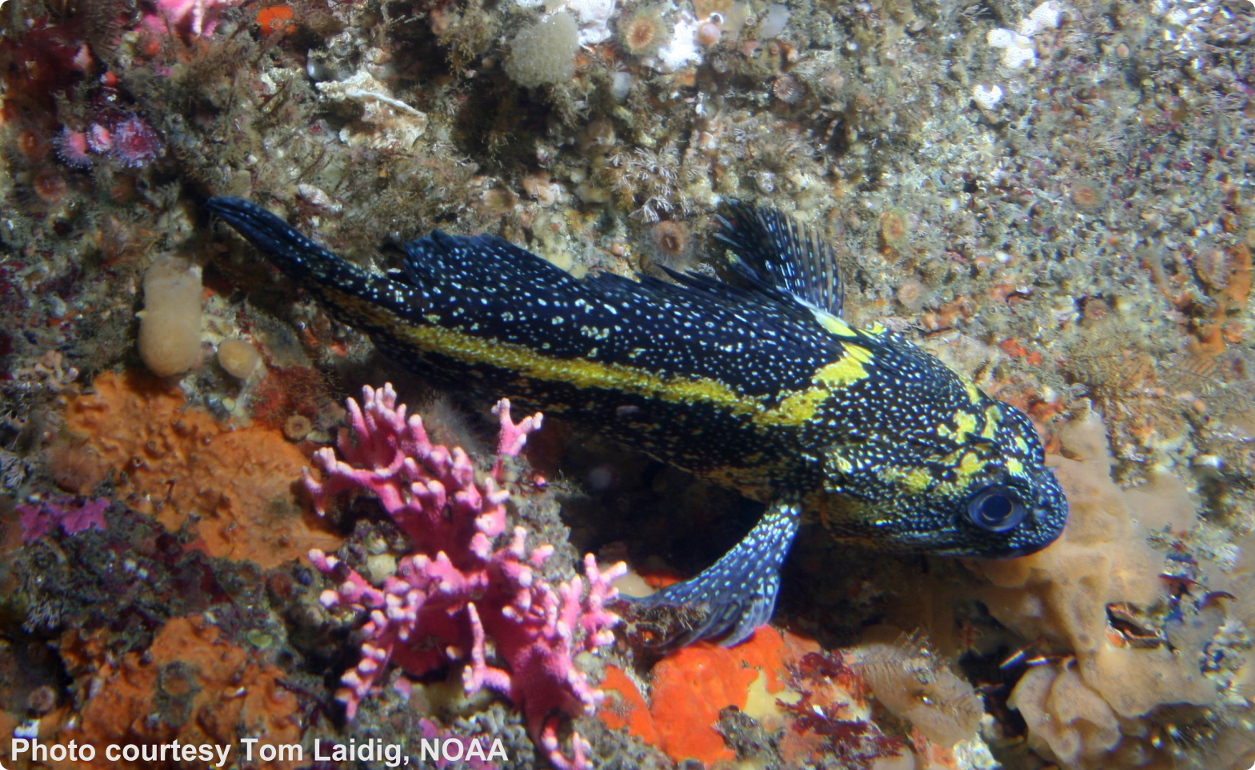
\includegraphics{cover_photo}~\\[1cm]
\pdftooltip{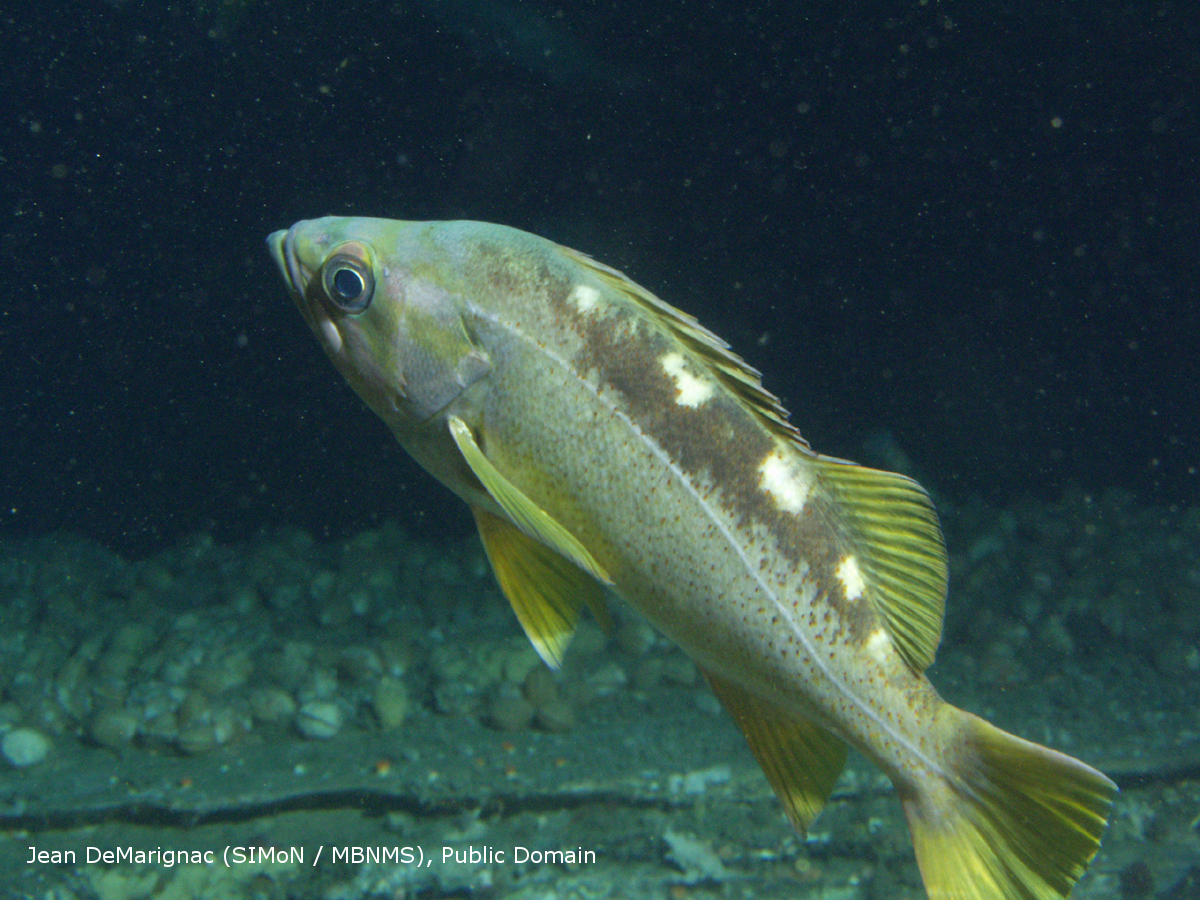
\includegraphics{Sebastes_flavidus_with_attribution}}{Yellowtail Rockfish}



Andi Stephens\textsuperscript{1}\\
Ian G. Taylor\textsuperscript{2}\\

\vspace{.5cm}

\small
\textsuperscript{1}Northwest Fisheries Science Center, U.S. Department of Commerce, National Oceanic and Atmospheric Administration, National Marine Fisheries Service, 2032 S.E. OSU Drive Newport, Oregon 97365\\

\vspace{.3cm}

\textsuperscript{2}Northwest Fisheries Science Center, U.S. Department of Commerce, National Oceanic and Atmospheric Administration, National Marine Fisheries Service, 2725 Montlake Boulevard East, Seattle, Washington 98112\\


\vspace{.5cm}

\vfill
DRAFT SAFE\\
Disclaimer: This information is distributed solely for the purpose of pre-dissemination
peer review under applicable information quality guidelines. It has not been formally
disseminated by NOAA Fisheries. It does not represent and should not be construed to
represent any agency determination or policy. 

\vspace{.3cm}
%Bottom of the page
%{\large \today}

\maketitle

\pagenumbering{roman}
\setcounter{page}{1}
\end{center}

{
\setcounter{tocdepth}{4}
\tableofcontents
}
\setlength{\parskip}{5mm plus1mm minus1mm} \pagebreak

\pagenumbering{arabic} \setcounter{page}{1}
\renewcommand{\thefigure}{\alph{figure}}
\renewcommand{\thetable}{\alph{table}}

\section*{Executive Summary}\label{executive-summary}
\addcontentsline{toc}{section}{Executive Summary}

\subsection*{Stock}\label{stock}
\addcontentsline{toc}{subsection}{Stock}

This assessment reports the status of the Yellowtail Rockfish
(\emph{Sebastes flavidus}) resource in U.S. waters off the coast of the
California, Oregon, and Washington using data through 2016.

The Pacific Fishery Management Council (PFMC) manages the U.S. fishery
as two stocks separated at Cape Mendocino, California (40\(^\circ\)
10'N). The northern stock has long been assessed on its own; the
southern stock is treated as part of the Southern Shelf Complex. This
assessment analyzes each stock independently, with the southern stock
extending southward to the U.S./Mexico border and the northern stock
extending northward to the U.S./Canada border.

The most recent fully integrated assessment (Wallace and Lai
\protect\hyperlink{ref-Wallace2005}{2005}), following the pattern of
prior assessments, included only the Northern stock which it divided
into three assessment areas with divisions at Cape Elizabeth
(47\(^\circ\) 20'N) and Cape Falcon (45\(^\circ\) 46'N). A data-moderate
assessment conducted in 2013 (Cope et al.
\protect\hyperlink{ref-Cope2013}{2013}) was the first to analyze the
southern stock, determining its contribution to the overfishing limit
(OFL) for the Southern Shelf Complex.

Since the 2005 assessment, reconstruction of historical catch by
Washington and Oregon makes any border but the state line (roughly
46\(^\circ\) N) incompatible with the data from those states.
Additionally, much of the groundfish catch landed in northern Oregon is
caught in Washington waters.

This assessment addresses the stock in two areas consistent with the
management border at Cape Mendocino. This is consistent, as well, with a
recent genetic analysis (Hess et al. n.d.) that found distinct stocks
north and south of Cape Mendocino but did not find stock differences
within the northern area.

\subsection*{Catches}\label{catches}
\addcontentsline{toc}{subsection}{Catches}

Catches from the Northern stock were divided into four categories:
commercial catch, bycatch in the at-sea hake fishery, recreational catch
in Oregon and California (north of 40\(^\circ\) 10'N), and recreational
catch in Washington. The first three of these fleets were entered in
metric tons, but the recreational catch from Washington was entered in
the model as numbers of fish with the average weight calculated
internally in the model from the weight-length relationship and the
length-compositions.

Catches from the Southern stock were divided into two categories:
commercial and recreational catch, both of which were entered as metric
tons.

\hl{Include: trends and current levels-include table for last ten years and graph with 
long term data}

Catch figures: (Figures \ref{fig:r4ss_catch_N}-\ref{fig:r4ss_catch_S})\\
Catch tables: (Tables \ref{tab:Exec_catch_N}-\ref{tab:Exec_catch_S})

\FloatBarrier

\FloatBarrier

\begin{figure}[htbp]
\centering
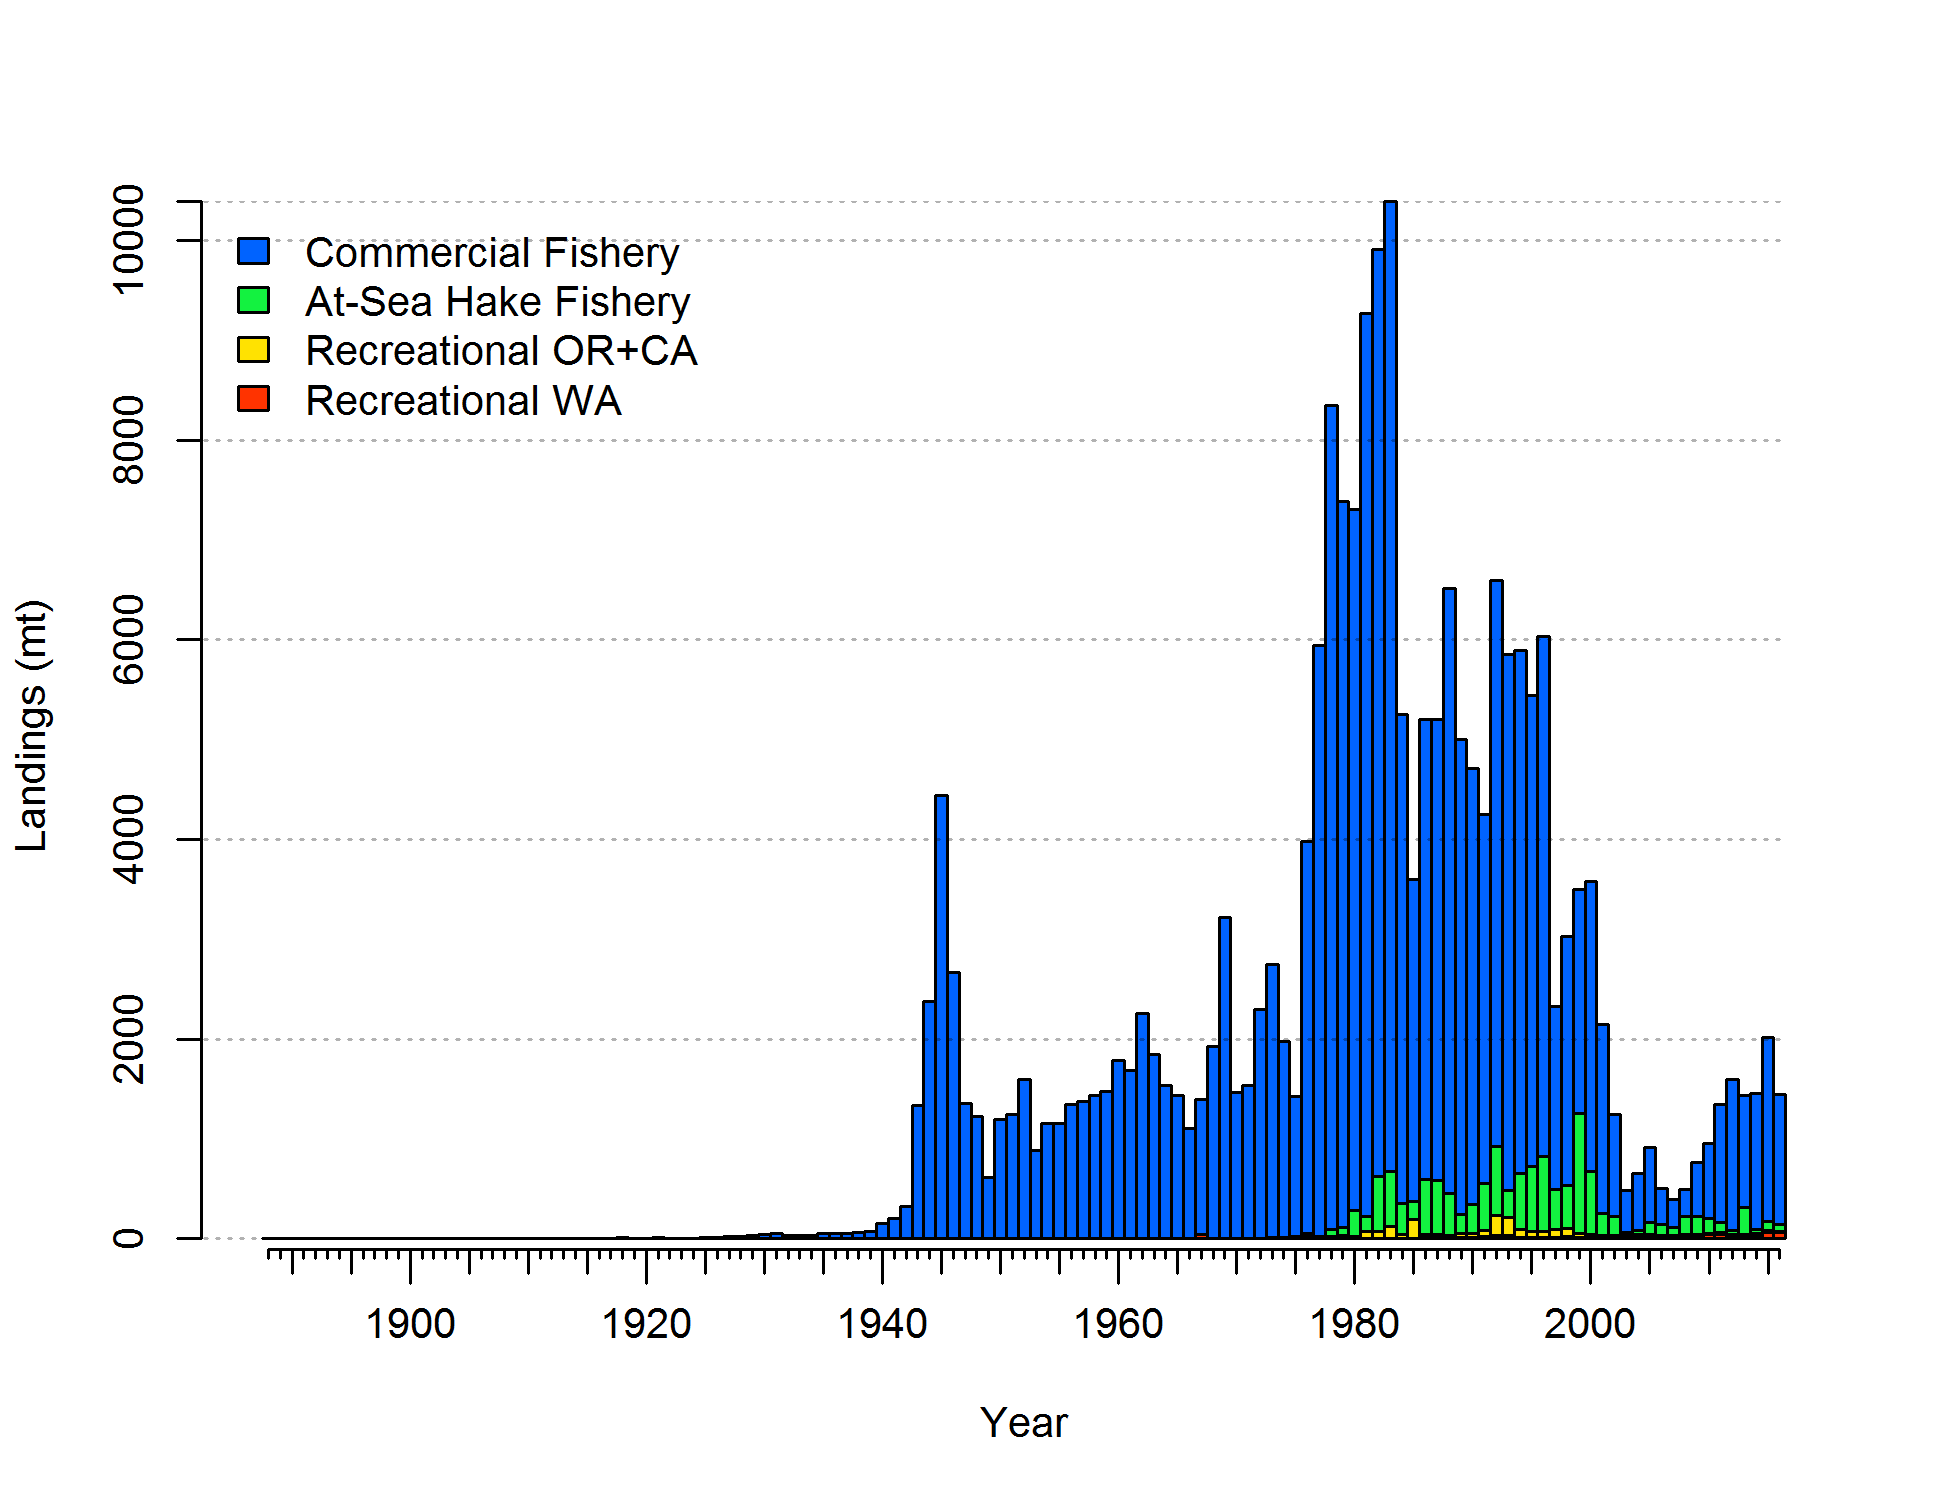
\includegraphics{r4ss/plots_mod1/catch2 landings stacked.png}
\caption{Estimated catch history of Yellowtail Rockfish in the Northern
model. Recreational catches in Washington are model estimates of total
weigth converted from input catch in numbers using model estimates of
growth and selectivity.\label{fig:r4ss_catch_N}}
\end{figure}

\begin{figure}[htbp]
\centering
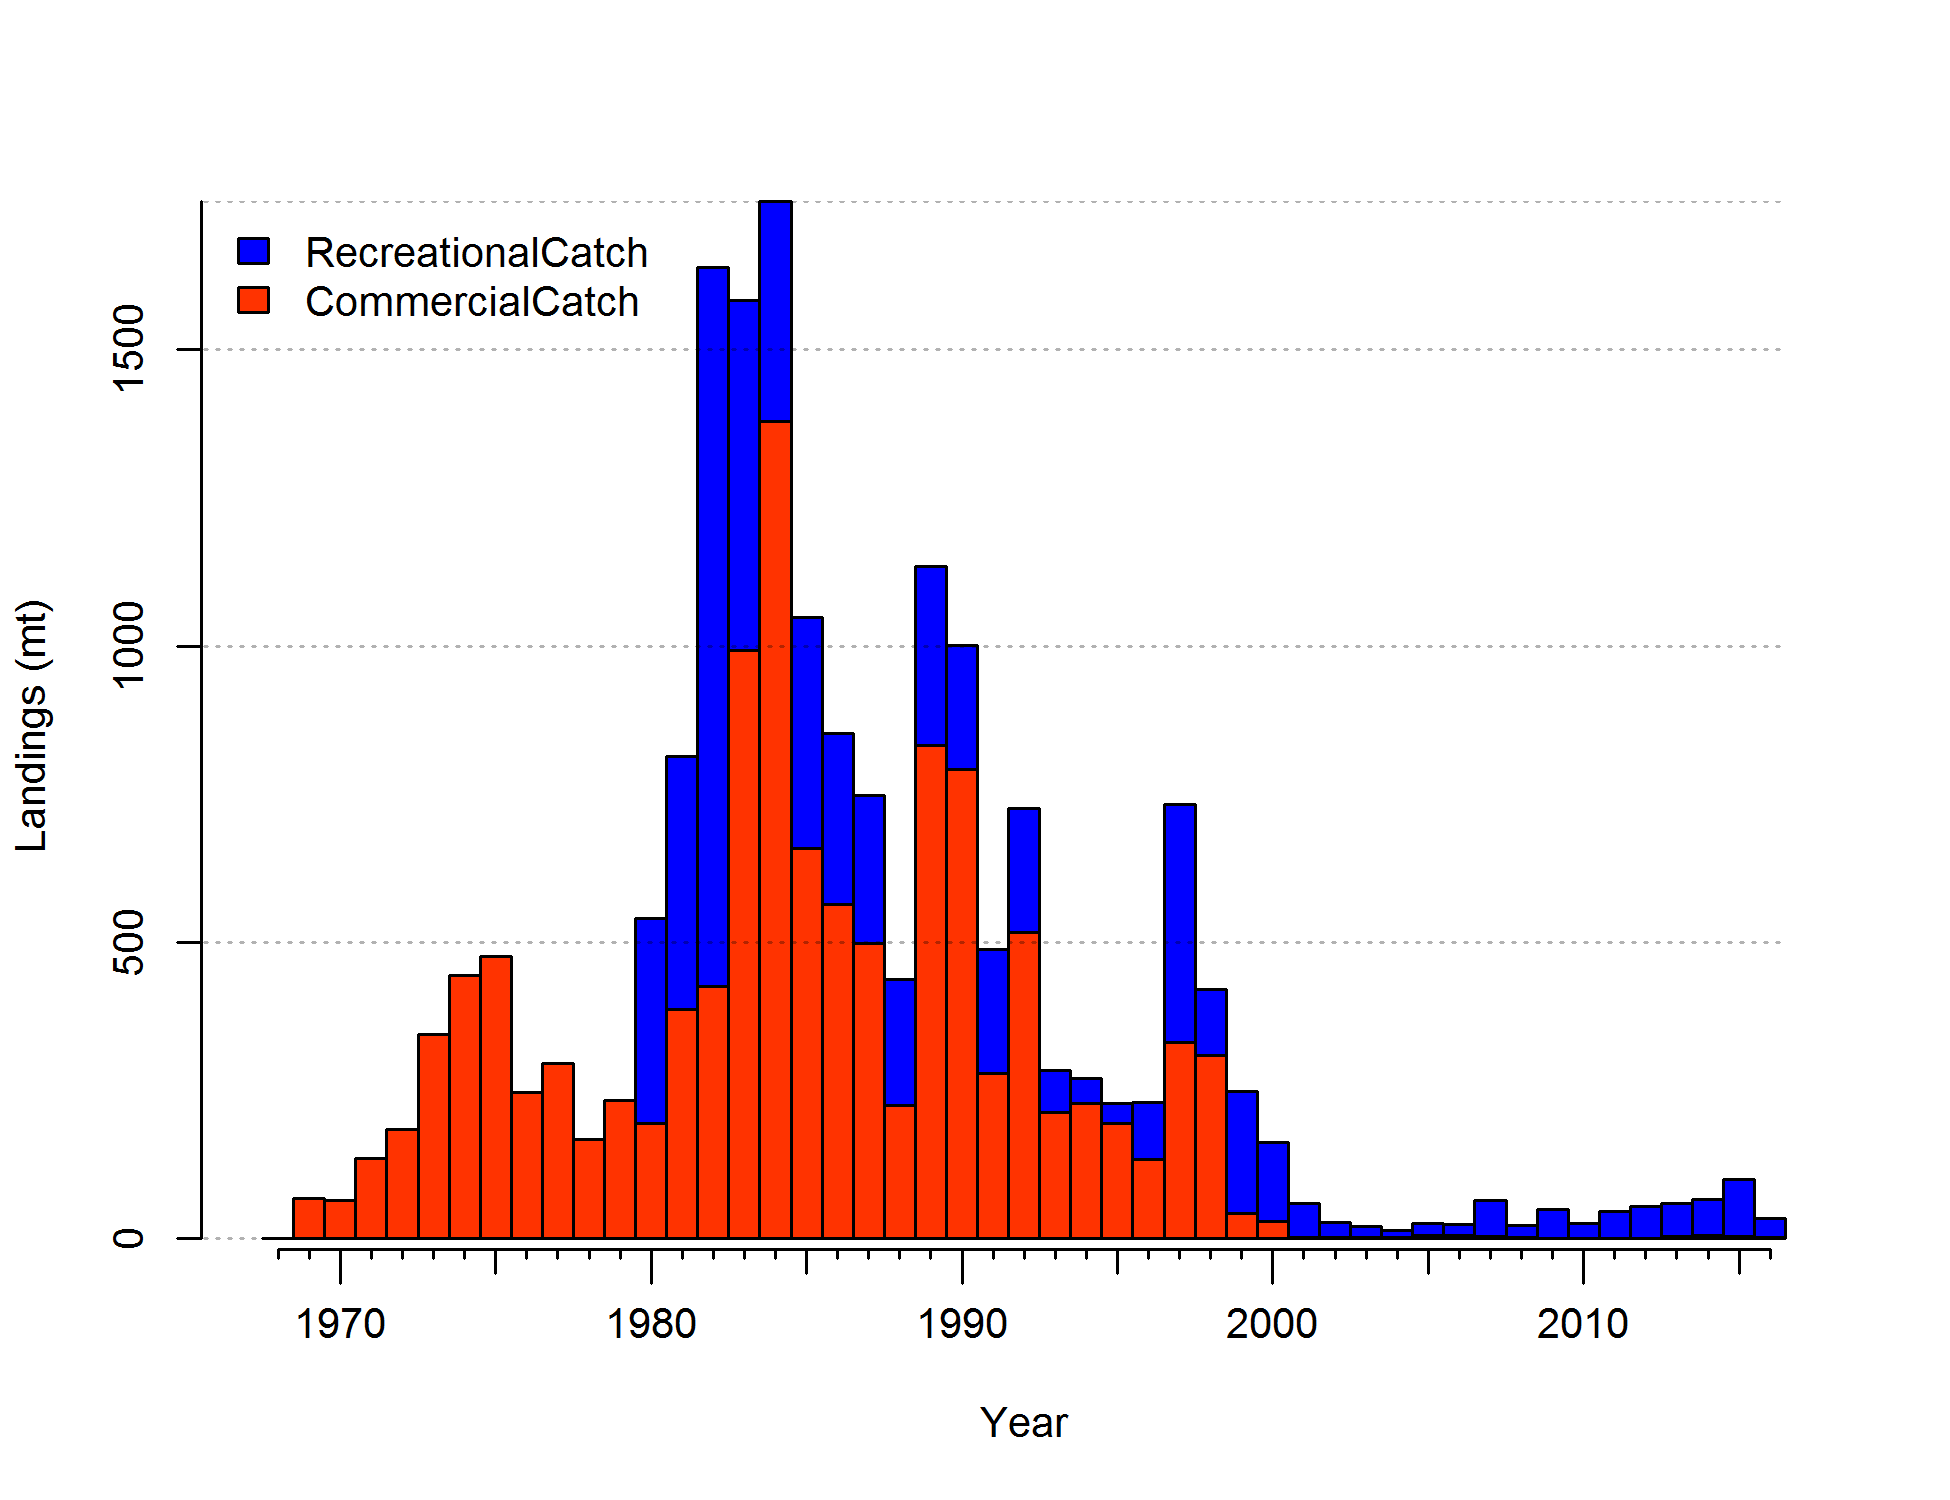
\includegraphics{r4ss/plots_mod2/catch2 landings stacked.png}
\caption{Estimated catch history of Yellowtail Rockfish in the Southern
model. \label{fig:r4ss_catch_S}}
\end{figure}

\begin{table}[ht]
\centering
\caption{Recent Yellowtail Rockfish catch by 
                                             fleet for the Northern stock 
                                             (north of 40$^\circ$ 10'N).} 
\label{tab:Exec_catch_N}
\begin{tabular}{l>{\centering}p{1.0in}>{\centering}p{1.0in}>{\centering}p{1.0in}>{\centering}p{1.0in}}
  \hline
Year & Commercial (t) & At-sea hake bycatch (t) & Recreational OR+CA (t) & Recreational WA (1000s) \\ 
  \hline
2007 & - & - & - & - \\ 
  2008 & - & - & - & - \\ 
  2009 & - & - & - & - \\ 
  2010 & - & - & - & - \\ 
  2011 & - & - & - & - \\ 
  2012 & - & - & - & - \\ 
  2013 & - & - & - & - \\ 
  2014 & - & - & - & - \\ 
  2015 & - & - & - & - \\ 
  2016 & - & - & - & - \\ 
   \hline
\end{tabular}
\end{table}

\begin{table}[ht]
\centering
\caption{Recent Yellowtail Rockfish catch by 
                                            fleet for the Southern stock 
                                             (south of 40$^\circ$ 10'N).} 
\label{tab:Exec_catch_S}
\begin{tabular}{l>{\centering}p{1.5in}>{\centering}p{1.5in}}
  \hline
Year & Recreational (t) & Commercial (t) \\ 
  \hline
2007 & - & - \\ 
  2008 & - & - \\ 
  2009 & - & - \\ 
  2010 & - & - \\ 
  2011 & - & - \\ 
  2012 & - & - \\ 
  2013 & - & - \\ 
  2014 & - & - \\ 
  2015 & - & - \\ 
  2016 & - & - \\ 
   \hline
\end{tabular}
\end{table}

\FloatBarrier

\newpage

\subsection*{Data and Assessment}\label{data-and-assessment}
\addcontentsline{toc}{subsection}{Data and Assessment}

\hl{Include: date of last assessment, type of assessment model, data available, new 
information, and information lacking.}

Yellowtail Rockfish was assessed north of Cape Mendocino in 2005 in a
fully integrated age-based assessment. A 2013 data-moderate assessment
was the first to address the southern stock (Cope et al.
\protect\hyperlink{ref-Cope2013}{2013}).

This assessment uses Stock Synthesis version 3.3. The Northern model
begins in 1889, with the assumption that the stock was at
\hl{an unfished equilibrium that year?} The Southern model begins in
1916, with the assumption that the stock was at
\hl{an unfished equilibrium that year?}

Map of assessment region: (Figure \ref{fig:assess_region_map_Exec_Sum}).

\begin{figure}[htbp]
\centering
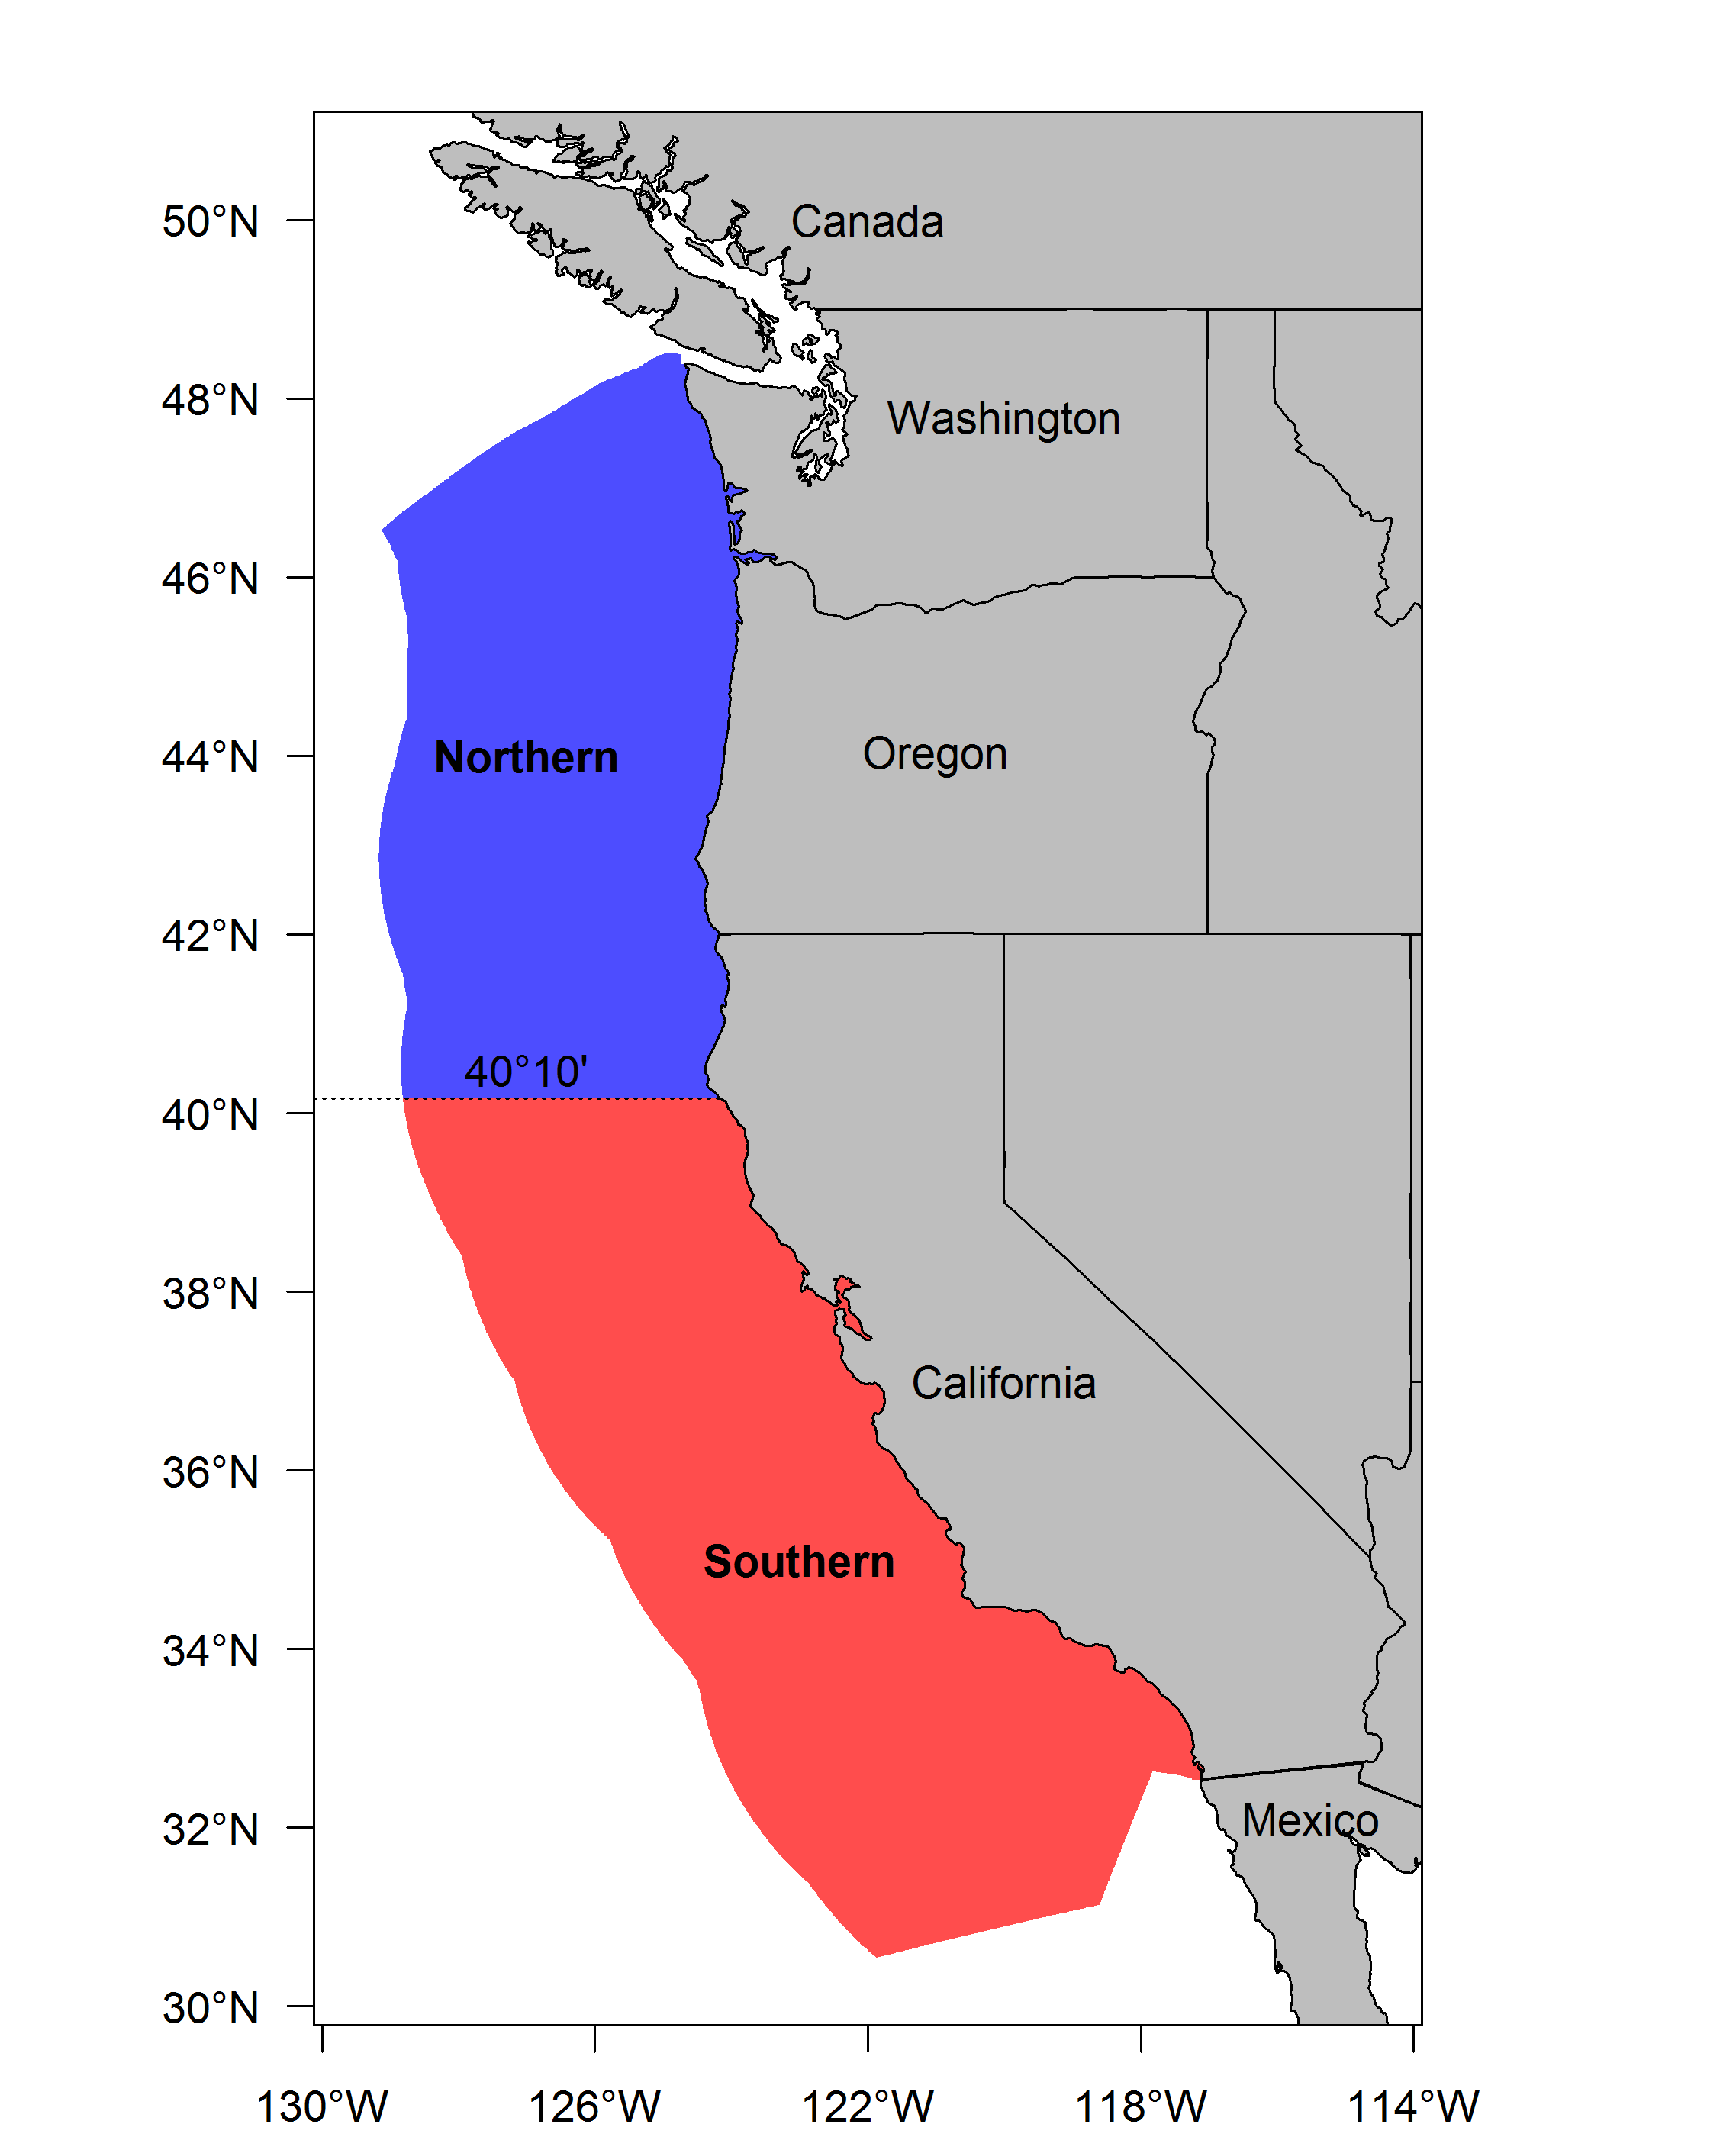
\includegraphics{Figures/assess_region_map_v2.png}
\caption{Map depicting the boundaries for the base-case model.
\label{fig:assess_region_map_Exec_Sum}}
\end{figure}

\FloatBarrier

\subsection*{Stock Biomass}\label{stock-biomass}
\addcontentsline{toc}{subsection}{Stock Biomass}

\hl{Include: trends and current levels relative to virgin or historic levels, 
description of uncertainty-include table for last 10 years and graph with 
long term estimates.}

Spawning output Figure: Figure \ref{fig:Spawnbio_all}\\
Spawning output Table(s): Table \ref{tab:SpawningDeplete_mod1}\\
Relative depletion Figure: Figure \ref{fig:RelDeplete_all}

Example text (remove Models 2 and 3 if not needed - if using, remove the
\# in-line comments!!!)\\
The estimated relative depletion level (spawning output relative to
unfished spawning output) of the the base-case model in 2016 is 56.7\%
(\textasciitilde{}95\% asymptotic interval: \(\pm\) 45.4\%-68.1\%)
(Figure \ref{fig:RelDeplete_all}).

The estimated relative depletion level of model 2 in 2016 is 98\%
(\textasciitilde{}95\% asymptotic interval: \(\pm\) 75.5\%-120\%)
(Figure \ref{fig:RelDeplete_all}).

The estimated relative depletion level of model 3 in 2016 is
(\textasciitilde{}95\% asymptotic interval: \(\pm\) ) (Figure
\ref{fig:RelDeplete_all}).

\FloatBarrier

\begin{table}[ht]
\centering
\caption{Recent trend in beginning of the 
                                      year spawning output and depletion for
                                      the Northern model for Yellowtail Rockfish.} 
\label{tab:SpawningDeplete_mod1}
\begin{tabular}{l>{\centering}p{1.3in}>{\centering}p{1.2in}>{\centering}p{1in}>{\centering}p{1.2in}}
  \hline
Year & Spawning Output (trillion eggs) & \~{} 95\% confidence interval & Estimated depletion & \~{} 95\% confidence interval \\ 
  \hline
2008 & 7.886 & (5.79-9.98) & 0.547 & (0.415-0.678) \\ 
  2009 & 8.289 & (6.13-10.45) & 0.575 & (0.442-0.707) \\ 
  2010 & 8.556 & (6.34-10.77) & 0.593 & (0.461-0.726) \\ 
  2011 & 8.652 & (6.41-10.9) & 0.600 & (0.469-0.731) \\ 
  2012 & 8.682 & (6.42-10.94) & 0.602 & (0.474-0.73) \\ 
  2013 & 8.591 & (6.34-10.85) & 0.596 & (0.472-0.719) \\ 
  2014 & 8.479 & (6.23-10.73) & 0.588 & (0.468-0.708) \\ 
  2015 & 8.374 & (6.13-10.62) & 0.580 & (0.464-0.697) \\ 
  2016 & 8.215 & (5.96-10.48) & 0.569 & (0.455-0.684) \\ 
  2017 & 8.186 & (5.9-10.47) & 0.567 & (0.454-0.681) \\ 
   \hline
\end{tabular}
\end{table}\begin{table}[ht]
\centering
\caption{Recent trend in 
                                             beginning of the year spawning output
                                             and depletion for the Southern model for Yellowtail Rockfish.} 
\label{tab:SpawningDeplete_mod2}
\begin{tabular}{l>{\centering}p{1.3in}>{\centering}p{1.2in}>{\centering}p{1in}>{\centering}p{1.2in}}
  \hline
Year & Spawning Output (trillion eggs) & \~{} 95\% confidence interval & Estimated depletion & \~{} 95\% confidence interval \\ 
  \hline
2008 & 3.934 & (0-10.7) & 0.678 & (0.529-0.828) \\ 
  2009 & 3.927 & (0-10.65) & 0.677 & (0.531-0.823) \\ 
  2010 & 3.953 & (0-10.7) & 0.681 & (0.537-0.826) \\ 
  2011 & 4.010 & (0-10.84) & 0.691 & (0.546-0.837) \\ 
  2012 & 4.088 & (0-11.03) & 0.705 & (0.557-0.852) \\ 
  2013 & 4.217 & (0-11.36) & 0.727 & (0.574-0.88) \\ 
  2014 & 4.384 & (0-11.79) & 0.756 & (0.598-0.913) \\ 
  2015 & 4.660 & (0-12.52) & 0.803 & (0.633-0.974) \\ 
  2016 & 5.083 & (0-13.64) & 0.876 & (0.685-1.068) \\ 
  2017 & 5.685 & (0-15.25) & 0.980 & (0.755-1.205) \\ 
   \hline
\end{tabular}
\end{table}

\FloatBarrier

\begin{figure}[htbp]
\centering
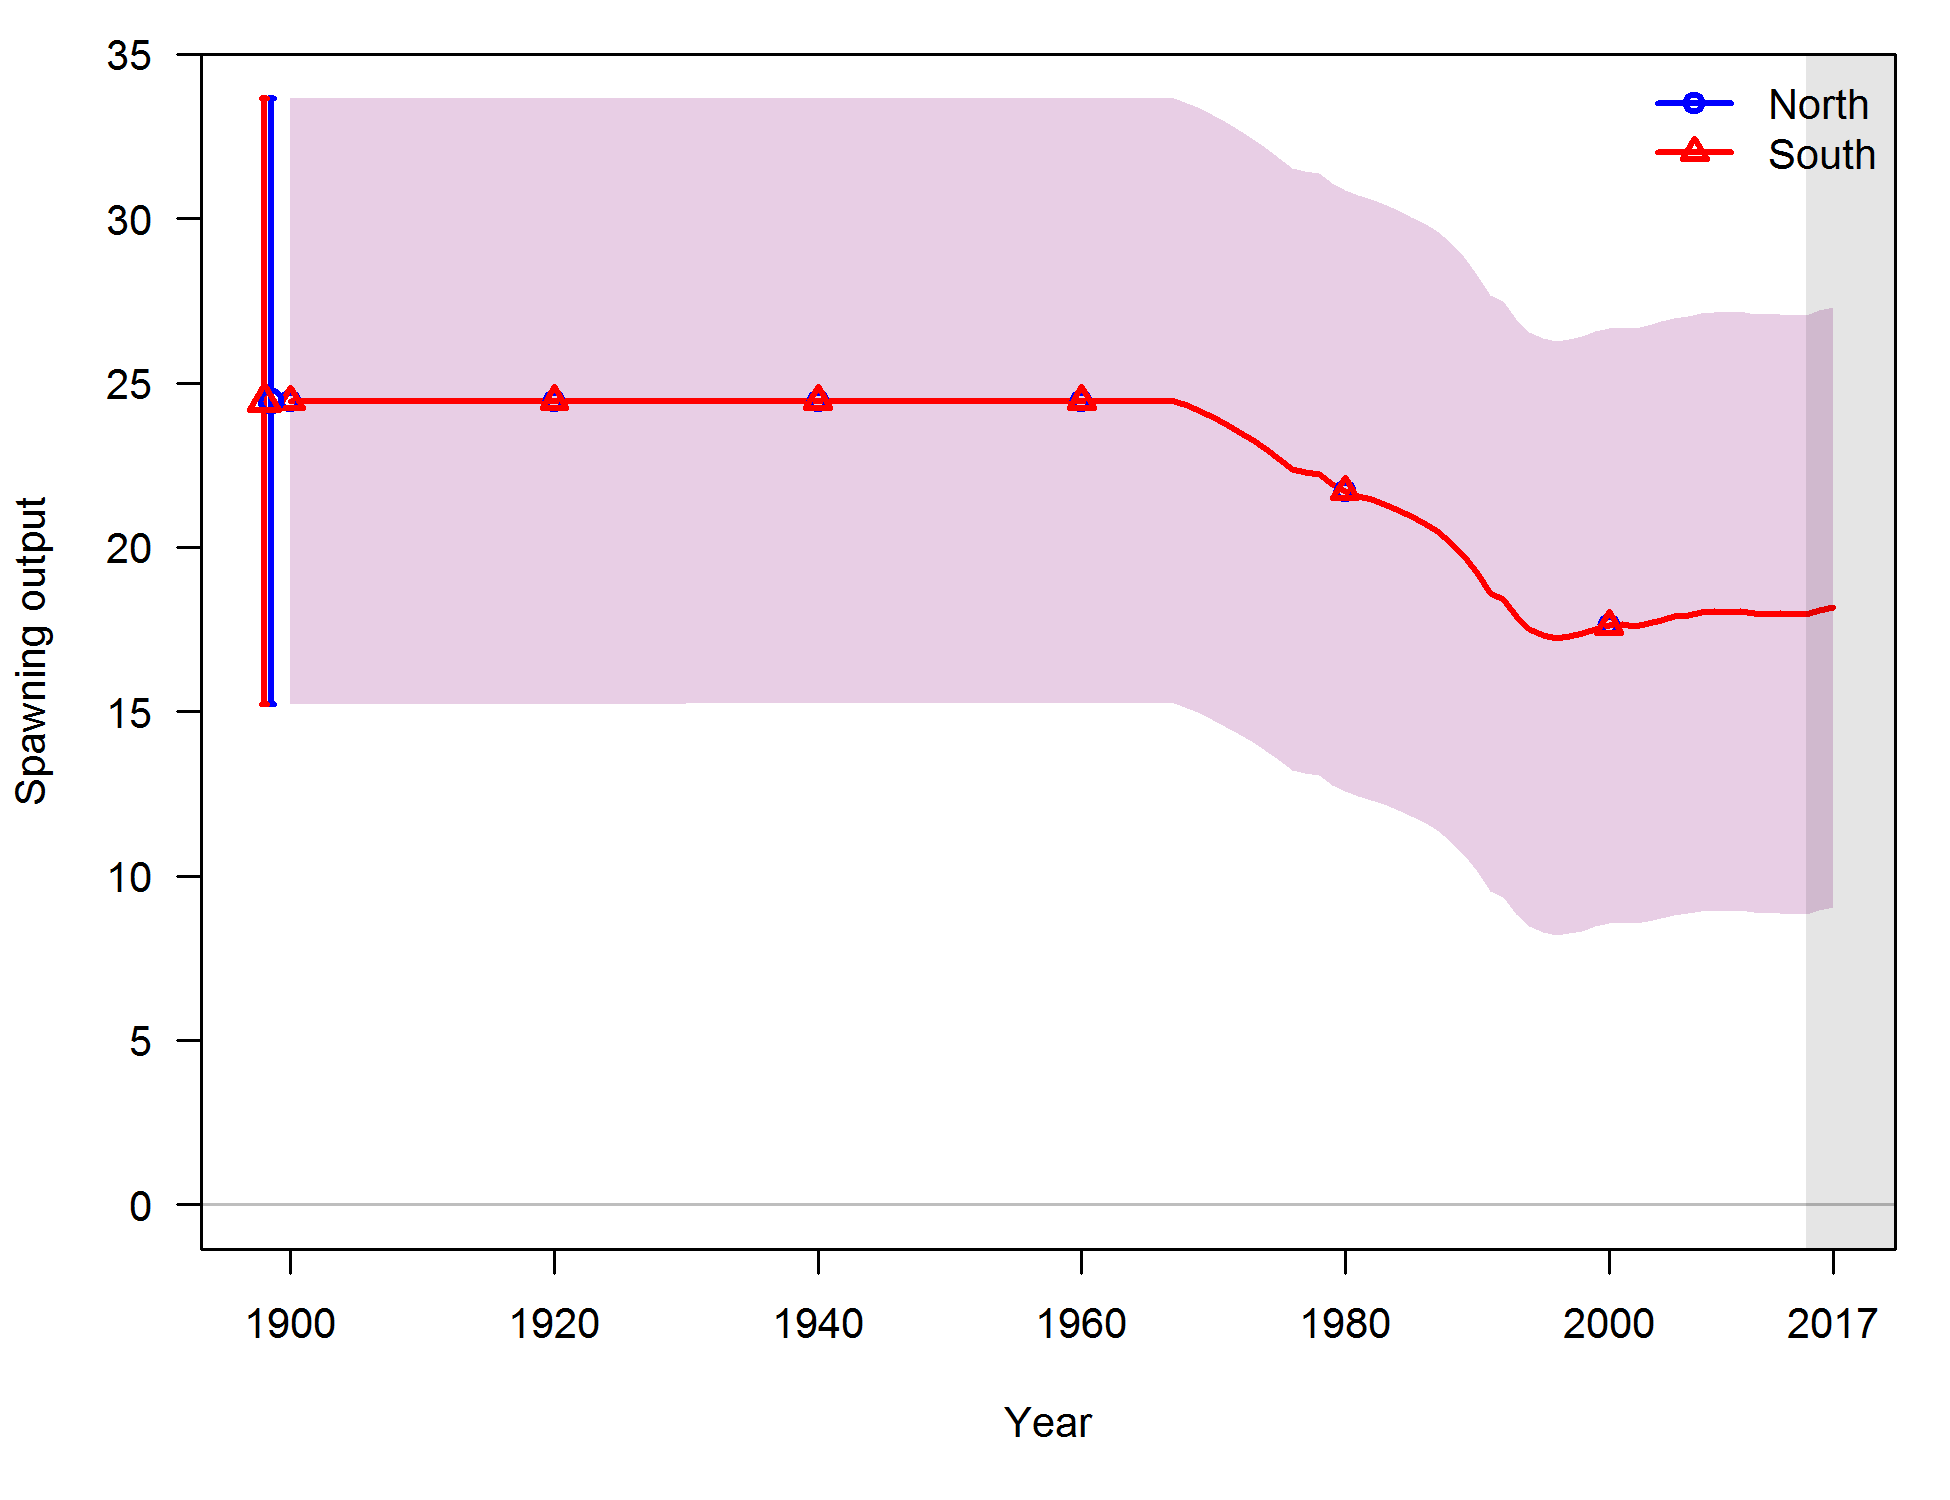
\includegraphics{r4ss/plots_compare/base_compare2_spawnbio_uncertainty.png}
\caption{Time series of spawning output trajectory (circles and line:
median; light broken lines: 95\% credibility intervals) for the base
case assessment model. \label{fig:Spawnbio_all}}
\end{figure}

\begin{figure}[htbp]
\centering
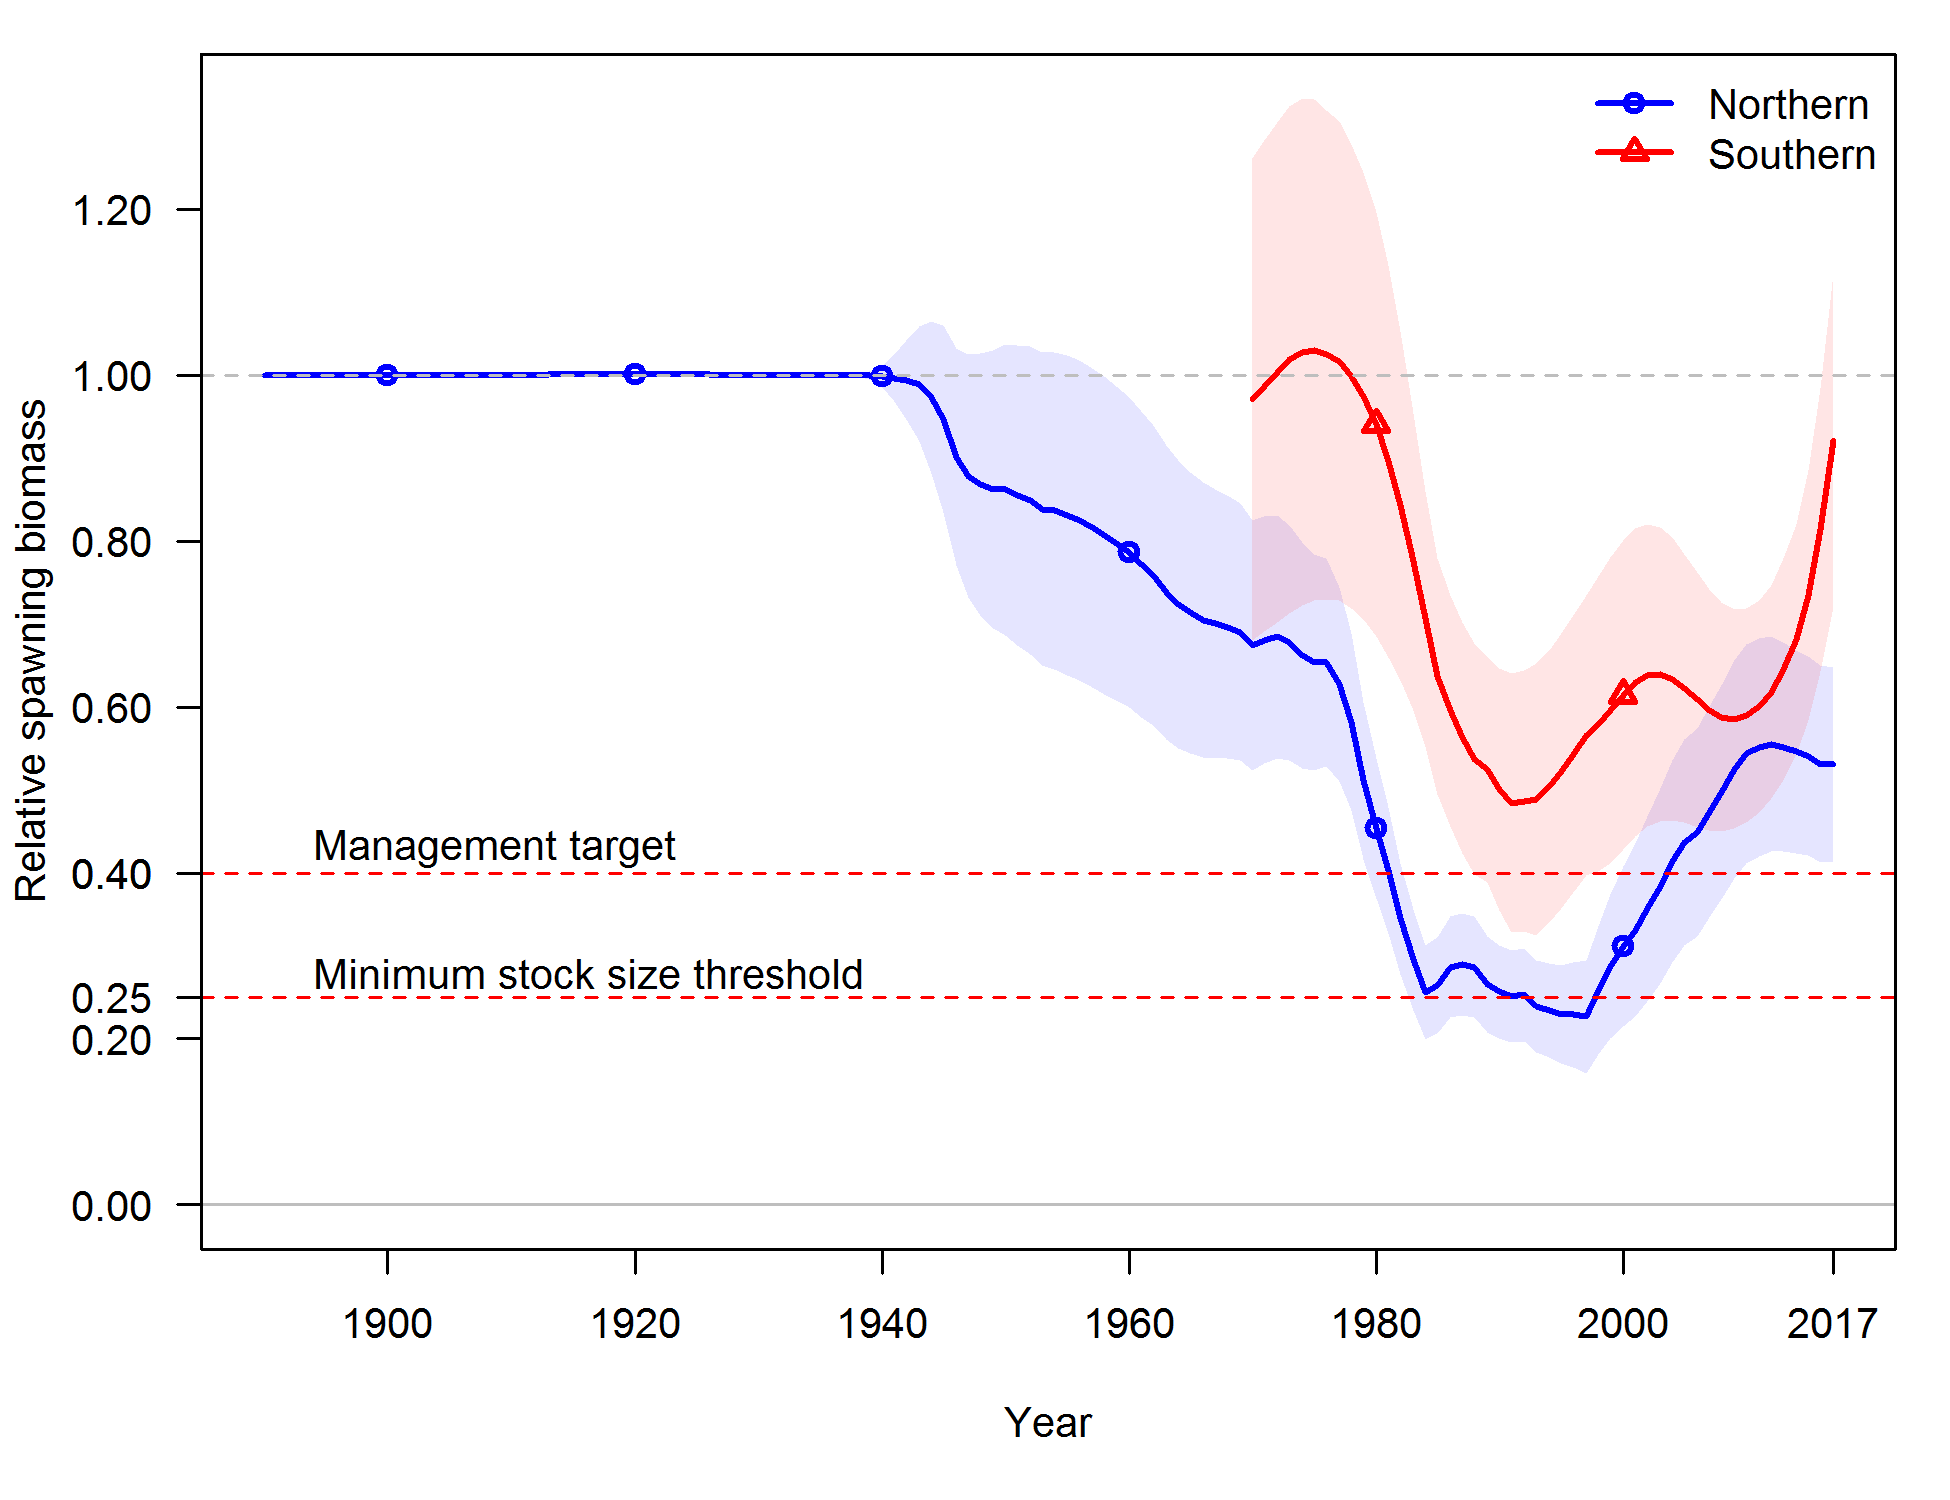
\includegraphics{r4ss/plots_compare/base_compare4_Bratio_uncertainty.png}
\caption{Estimated relative depletion with approximate 95\% asymptotic
confidnce intervals (dashed lines) for the base case assessment model.
\label{fig:RelDeplete_all}}
\end{figure}

\FloatBarrier

\subsection*{Recruitment}\label{recruitment}
\addcontentsline{toc}{subsection}{Recruitment}

\hl{Include: trends and current levels relative to virgin or historic levels-include 
table for last 10 years and graph with long term estimates.}

Recruitment Figure: (Figure \ref{fig:Recruits_all})\\
Recruitment Tables: (Tables \ref{tab:Recruit_mod1},
\ref{tab:Recruit_mod2} and \ref{tab:Recruit_mod3})

\begin{table}[ht]
\centering
\caption{Recent recruitment for the Northern model.} 
\label{tab:Recruit_mod1}
\begin{tabular}{>{\centering}p{.8in}>{\centering}p{1.6in}>{\centering}p{1.3in}}
  \hline
Year & Estimated Recruitment (millions) & \~{} 95\% confidence interval \\ 
  \hline
2008 & 41.17 & (25.53 - 66.41) \\ 
  2009 & 12.42 & (6.11 - 25.24) \\ 
  2010 & 26.22 & (14.25 - 48.26) \\ 
  2011 & 17.76 & (8.17 - 38.58) \\ 
  2012 & 18.73 & (7.45 - 47.06) \\ 
  2013 & 30.71 & (10.59 - 89.07) \\ 
  2014 & 28.43 & (9.78 - 82.61) \\ 
  2015 & 28.52 & (10.06 - 80.85) \\ 
  2016 & 28.31 & (10 - 80.14) \\ 
  2017 & 28.29 & (9.99 - 80.09) \\ 
   \hline
\end{tabular}
\end{table}\begin{table}[ht]
\centering
\caption{Recent recruitment for the Southern model.} 
\label{tab:Recruit_mod2}
\begin{tabular}{>{\centering}p{.8in}>{\centering}p{1.6in}>{\centering}p{1.3in}}
  \hline
Year & Estimated Recruitment (millions) & \~{} 95\% confidence interval \\ 
  \hline
2008 & 234.32 & (48.85 - 1124.05) \\ 
  2009 & 66.93 & (8.28 - 541.34) \\ 
  2010 & 170.66 & (28.63 - 1017.09) \\ 
  2011 & 81.72 & (11.33 - 589.32) \\ 
  2012 & 59.53 & (8.75 - 404.76) \\ 
  2013 & 62.96 & (10.56 - 375.27) \\ 
  2014 & 46.19 & (7.64 - 279.12) \\ 
  2015 & 37.77 & (6.4 - 222.96) \\ 
  2016 & 35.70 & (5.83 - 218.81) \\ 
  2017 & 36.73 & (6 - 225) \\ 
   \hline
\end{tabular}
\end{table}

\FloatBarrier

\begin{figure}[htbp]
\centering
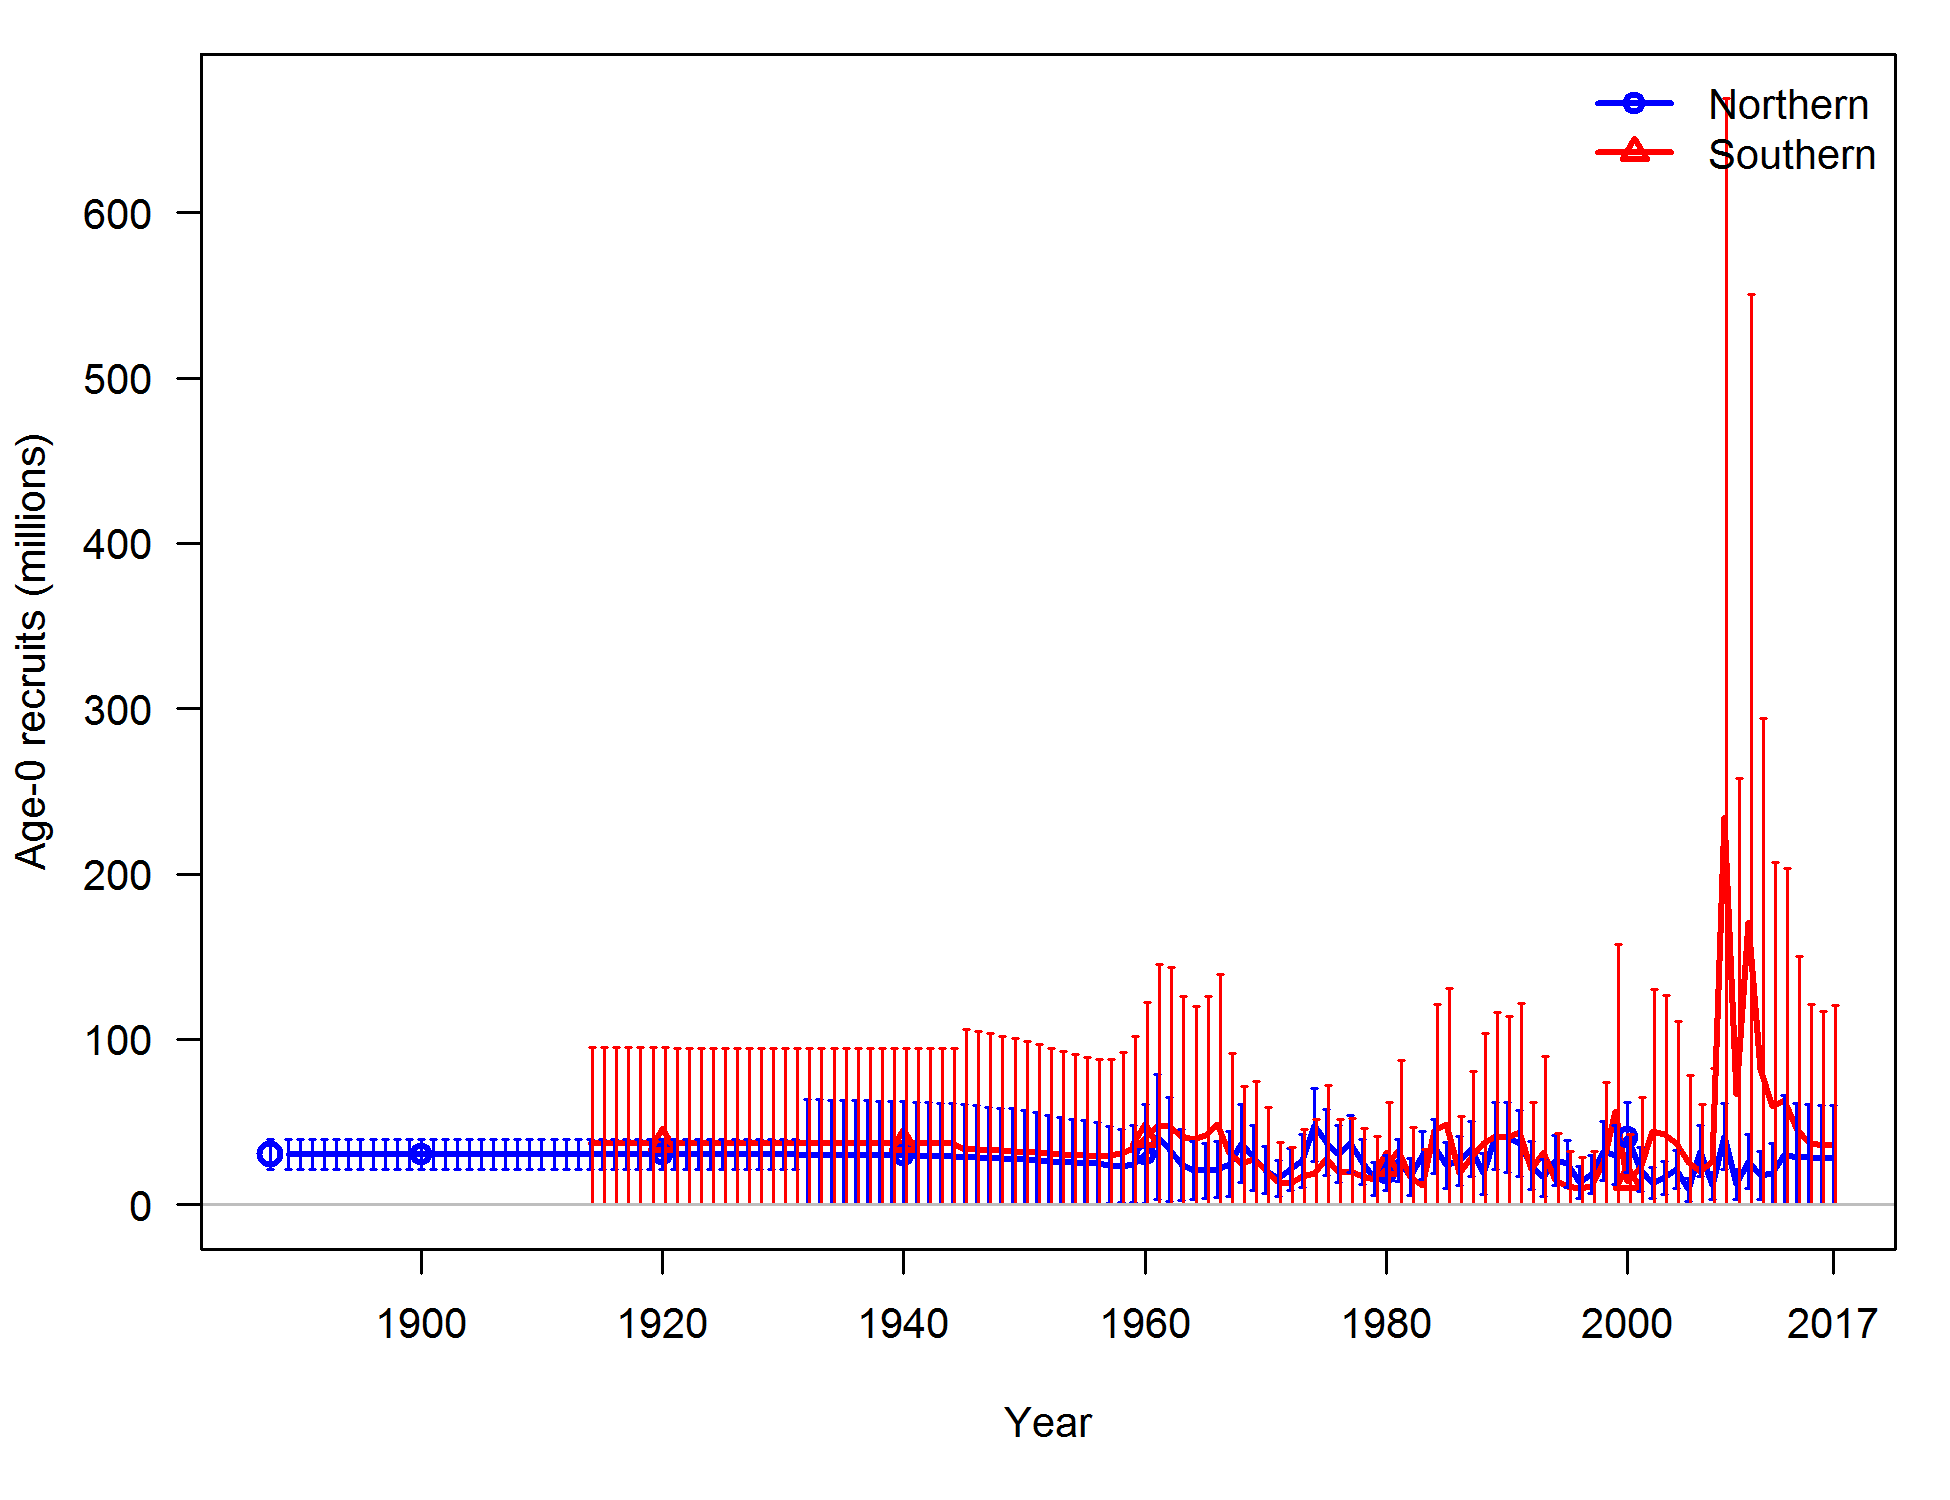
\includegraphics{r4ss/plots_compare/base_compare8_recruits_uncertainty.png}
\caption{Time series of estimated Yellowtail Rockfish recruitments for
the base-case model with 95\% confidence or credibility intervals.
\label{fig:Recruits_all}}
\end{figure}

\FloatBarrier

\subsection*{Exploitation status}\label{exploitation-status}
\addcontentsline{toc}{subsection}{Exploitation status}

\hl{Include: exploitation rates (i.e., total catch divided by exploitable biomass, or the annual SPR harvest rate) – include a table with the last 10 years of data and a graph showing the trend in fishing mortality relative to the target (y-axis) plotted against the trend in biomass relative to the target (x-axis).}

Exploitation Tables: Table \ref{tab:SPR_Exploit_mod1}, Table
\ref{tab:SPR_Exploit_mod2}, Table \ref{tab:SPR_Exploit_mod3}
Exploitation Figure: Figure \ref{fig:SPR_all}).

A summary of Yellowtail Rockfish exploitation histories for base model
is provided as Figure \ref{fig:Phase_all}.

\FloatBarrier

\begin{table}[ht]
\centering
\caption{Recent trend in spawning potential 
                                        ratio and exploitation for Yellowtail Rockfish in the Northern model.  Fishing intensity is (1-SPR) 
                                        divided by 50\% (the SPR target) and exploitation 
                                        is F divided by F\textsubscript{SPR}.} 
\label{tab:SPR_Exploit_mod1}
\begin{tabular}{l>{\centering}p{1in}>{\centering}p{1.2in}>{\centering}p{1in}>{\centering}p{1.2in}}
  \hline
Year & Fishing intensity & \~{} 95\% confidence interval & Exploitation rate & \~{} 95\% confidence interval \\ 
  \hline
2007 & 0.30 & (0.11-0.49) & 0.01 & (0-0.02) \\ 
  2008 & 0.19 & (0.13-0.25) & 0.01 & (0-0.01) \\ 
  2009 & 0.35 & (0.22-0.48) & 0.01 & (0.01-0.02) \\ 
  2010 & 0.47 & (0.24-0.7) & 0.02 & (0.01-0.03) \\ 
  2011 & 0.41 & (0.3-0.52) & 0.02 & (0.01-0.02) \\ 
  2012 & 0.47 & (0.35-0.59) & 0.02 & (0.01-0.02) \\ 
  2013 & 0.44 & (0.33-0.56) & 0.02 & (0.01-0.02) \\ 
  2014 & 0.45 & (0.33-0.57) & 0.02 & (0.01-0.02) \\ 
  2015 & 0.59 & (0.44-0.73) & 0.02 & (0.02-0.03) \\ 
  2016 & 0.46 & (0.34-0.57) & 0.02 & (0.01-0.02) \\ 
   \hline
\end{tabular}
\end{table}\begin{table}[ht]
\centering
\caption{Recent trend in spawning potential 
                                        ratio and exploitation for Yellowtail Rockfish in the Southern model. Fishing intensity is (1-SPR) 
                                        divided by 50\% (the SPR target) and exploitation 
                                        is F divided by F\textsubscript{SPR}.} 
\label{tab:SPR_Exploit_mod2}
\begin{tabular}{l>{\centering}p{1in}>{\centering}p{1.2in}>{\centering}p{1in}>{\centering}p{1.2in}}
  \hline
Year & Fishing intensity & \~{} 95\% confidence interval & Exploitation rate & \~{} 95\% confidence interval \\ 
  \hline
2007 & 0.02 & (0-0.06) & 0.00 & (0-0) \\ 
  2008 & 0.01 & (0-0.02) & 0.00 & (0-0) \\ 
  2009 & 0.02 & (0-0.05) & 0.00 & (0-0) \\ 
  2010 & 0.01 & (0-0.02) & 0.00 & (0-0) \\ 
  2011 & 0.01 & (0-0.04) & 0.00 & (0-0) \\ 
  2012 & 0.01 & (0-0.04) & 0.00 & (0-0) \\ 
  2013 & 0.01 & (0-0.04) & 0.00 & (0-0) \\ 
  2014 & 0.01 & (0-0.04) & 0.00 & (0-0) \\ 
  2015 & 0.02 & (0-0.05) & 0.00 & (0-0) \\ 
  2016 & 0.01 & (0-0.02) & 0.00 & (0-0) \\ 
   \hline
\end{tabular}
\end{table}

\FloatBarrier

\begin{figure}[htbp]
\centering
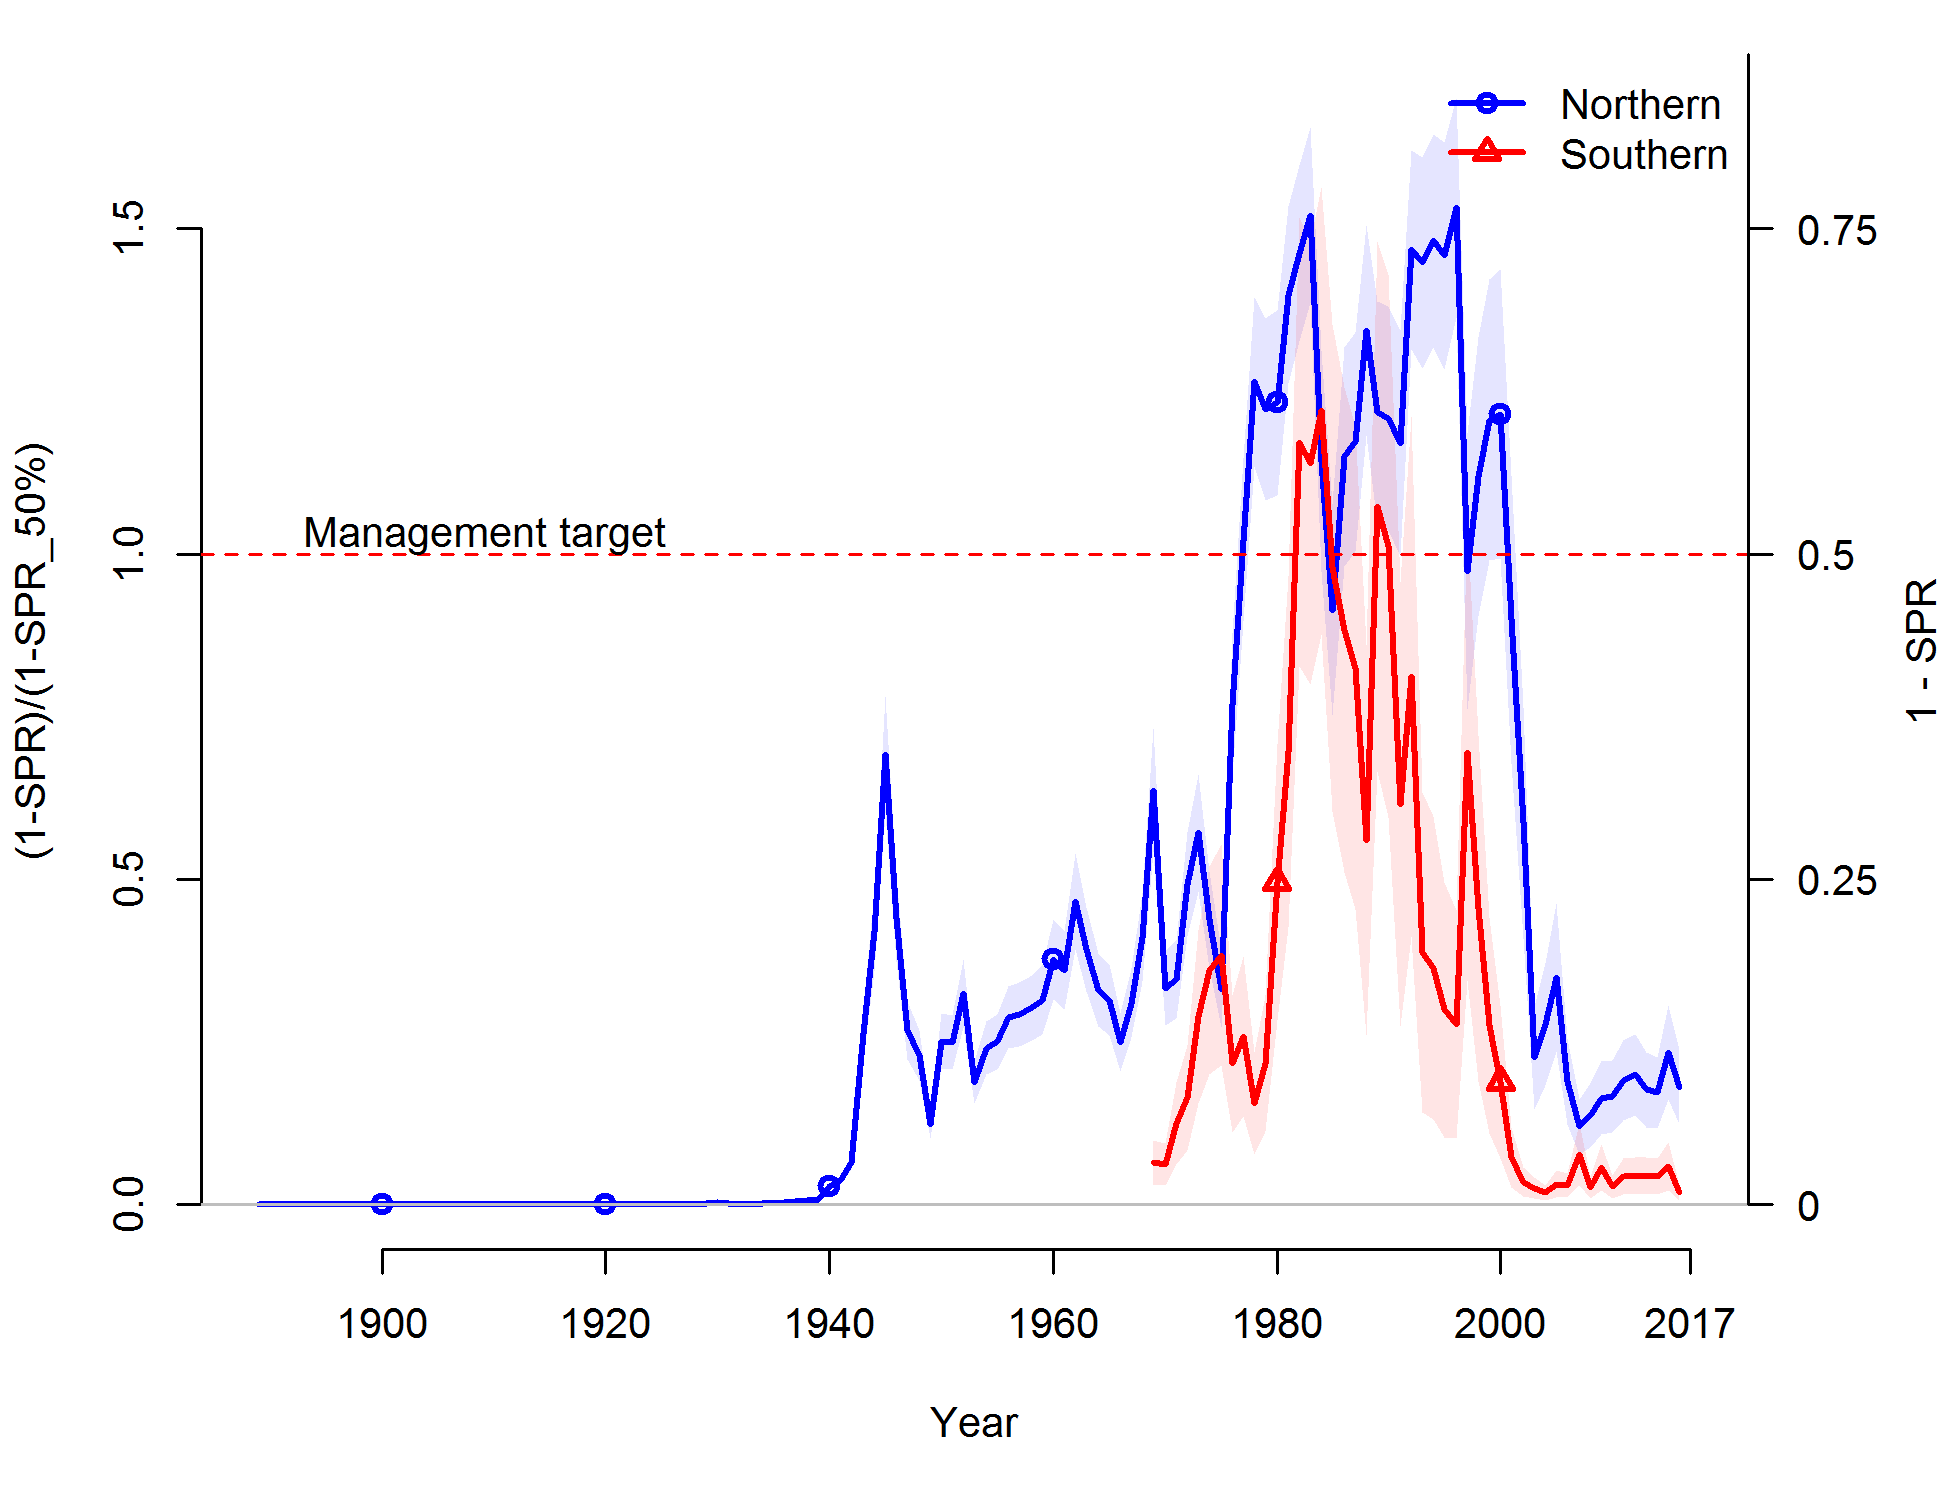
\includegraphics{r4ss/plots_compare/base_compare6_SPRratio_uncertainty.png}
\caption{Estimated spawning potential ratio (SPR) for the base-case
model. One minus SPR is plotted so that higher exploitation rates occur
on the upper portion of the y-axis. The management target is plotted as
a red horizontal line and values above this reflect harvests in excess
of the overfishing proxy based on the SPR\textsubscript{50\%} harvest
rate. The last year in the time series is 2016. \label{fig:SPR_all}}
\end{figure}

\begin{figure}[htbp]
\centering
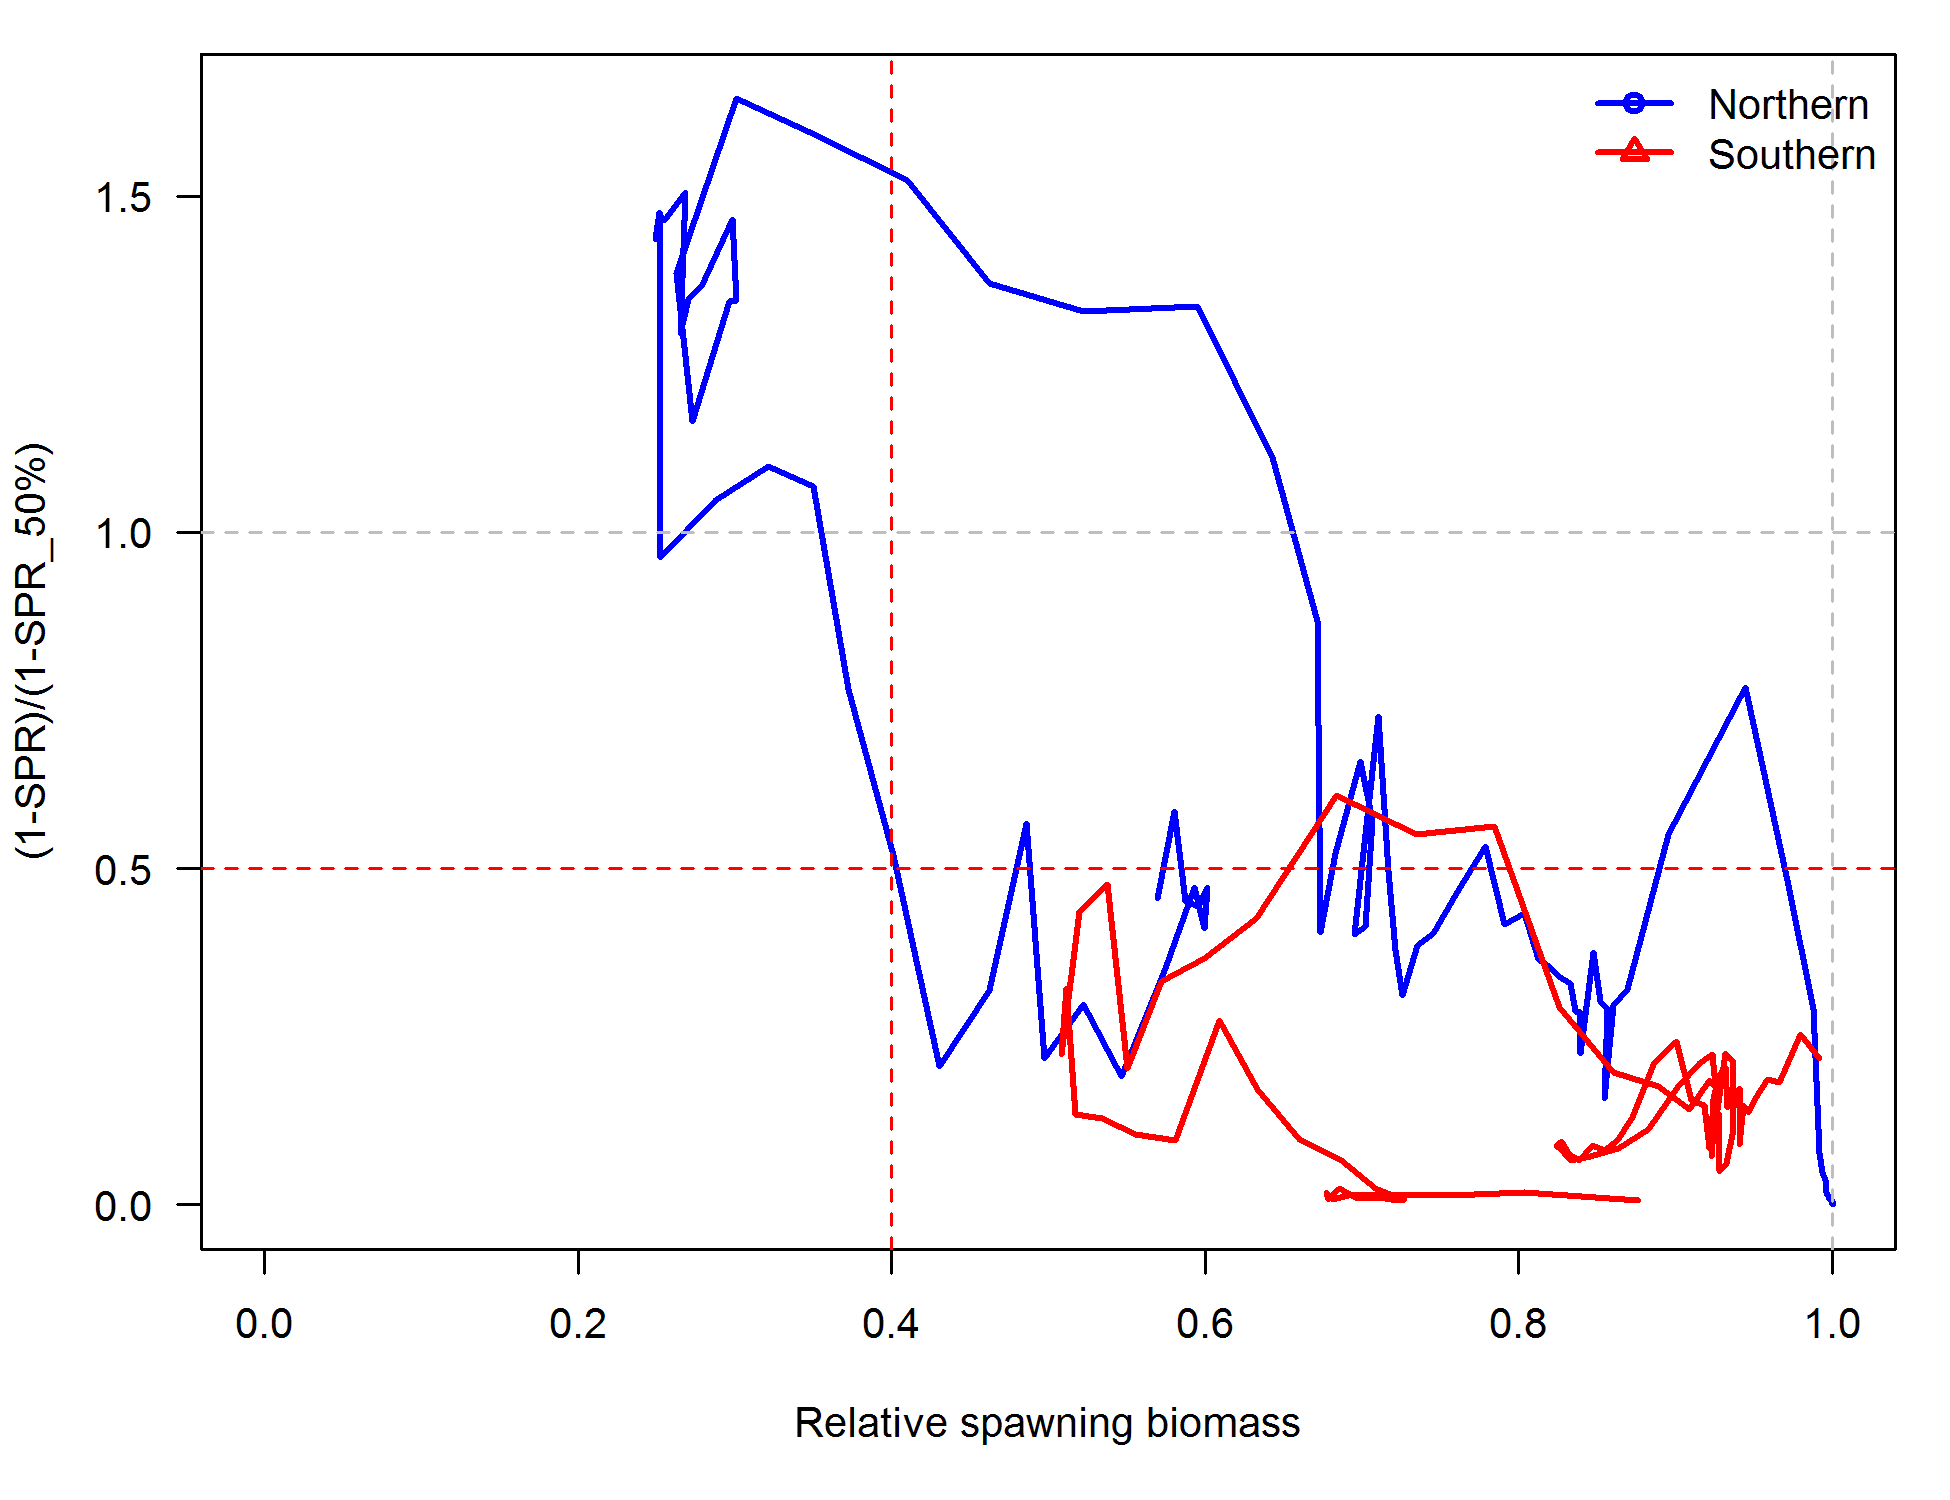
\includegraphics{r4ss/plots_compare/base_compare13_phase_plot.png}
\caption{Phase plot of estimated relative (1-SPR) vs.~relative spawning
biomass for the base case model. The relative (1-SPR) is (1-SPR) divided
by 50\% (the SPR target). Relative depletion is the annual spawning
biomass divided by the unfished spawning biomass. \label{fig:Phase_all}}
\end{figure}

\FloatBarrier

\subsection*{Ecosystem Considerations}\label{ecosystem-considerations}
\addcontentsline{toc}{subsection}{Ecosystem Considerations}

In this assessment, ecosystem considerations were\ldots{}..

\subsection*{Reference Points}\label{reference-points}
\addcontentsline{toc}{subsection}{Reference Points}

\hl{Include:} management targets and definition of overfishing,
including the harvest rate that brings the stock to equilibrium at
\(B_{40\%}\) (the \(B_{MSY}\) proxy) and the equilibrium stock size that
results from fishing at the default harvest rate (the \(F_{MSY}\)
proxy). Include a summary table that compares estimated reference points
for SSB, SPR, Exploitation Rate and Yield based on SSBproxy for MSY,
SPRproxy for MSY, and estimated MSY values

\hl{Write intro paragraph....and remove text for Models 2 and 3 if not needed}

This stock assessment estimates that Yellowtail Rockfish in the Northern
model are above the biomass target, but above the minimum stock size
threshold. \hl{Add sentence about spawning output trend.} The estimated
relative depletion level for \hl{Model 1} in 2016 is 56.7\%
(\textasciitilde{}95\% asymptotic interval: \(\pm\) 45.4\%-68.1\%,
corresponding to an unfished spawning output of 8.18588 trillion eggs
(\textasciitilde{}95\% asymptotic interval: 5.9-10.47 trillion eggs) of
spawning output in the base model (Table \ref{tab:Ref_pts_mod1}).
Unfished age 4+ biomass was estimated to be 132.7 mt in the base case
model. The target spawning output based on the biomass target
(\(SB_{40\%}\)) is 5.8 trillion eggs, which gives a catch of 4116.9 mt.
Equilibrium yield at the proxy \(F_{MSY}\) harvest rate corresponding to
\(SPR_{50\%}\) is 3882.8 mt.

This stock assessment estimates that Yellowtail Rockfish in the Southern
model are above the biomass target, but above the minimum stock size
threshold. \hl{Add sentence about spawning output trend.} The estimated
relative depletion level for \hl{Model 2} in 2016 is 98\%
(\textasciitilde{}95\% asymptotic interval: \(\pm\) 75.5\%-120\%),
corresponding to an unfished spawning output of 5.68452 trillion eggs
(\textasciitilde{}95\% asymptotic interval: ) of spawning output in the
base model (Table \ref{tab:Ref_pts_mod2}). Unfished age 4+ biomass was
estimated to be 117.6 mt in the base case model. The target spawning
output based on the biomass target (\(SB_{40\%}\)) is 2.3 trillion eggs,
which gives a catch of mt. Equilibrium yield at the proxy \(F_{MSY}\)
harvest rate corresponding to \(SPR_{50\%}\) is 3136.4 mt.

This stock assessment estimates that Yellowtail Rockfish in the are

the biomass target, but\\
the minimum stock size threshold.
\hl{Add sentence about spawning output trend.} The estimated relative
depletion level or \hl{Model 3} in 2016 is (\textasciitilde{}95\%
asymptotic interval: \(\pm\) ), corresponding to an unfished spawning
output of (\textasciitilde{}95\% asymptotic interval: ) of spawning
output in the base model (Table \ref{tab:Ref_pts_mod3}). Unfished age 4+
biomass was estimated to be mt in the base case model. The target
spawning output based on the biomass target (\(SB_{40\%}\)) is , which
gives a catch of mt. Equilibrium yield at the proxy \(F_{MSY}\) harvest
rate corresponding to \(SPR_{50\%}\) is mt.

\FloatBarrier

\begin{table}[ht]
\centering
\caption{Summary of reference 
                                      points and management quantities for the 
                                      base case Northern model.} 
\label{tab:Ref_pts_mod1}
\begin{tabular}{>{\raggedright}p{4.1in}>{\centering}p{.65in}>{\centering}p{1.4in}}
  \hline
\textbf{Quantity} & \textbf{Estimate} & \textbf{\~95\%  Confidence Interval} \\ 
  \hline
Unfished spawning output (trillion eggs) & 14.4 & (12.2-16.7) \\ 
  Unfished age 4+ biomass (1000 mt) & 132.7 & (113.8-151.7) \\ 
  Unfished recruitment (R0, millions) & 30.3 & (21.2-39.5) \\ 
  Spawning output(2016 trillion eggs) & 8.2 & (6-10.5) \\ 
  Relative Spawning Biomass (depletion)2016) & 0.5694 & (0.4547-0.6842) \\ 
  \textbf{$\text{Reference points based on } \mathbf{SB_{40\%}}$} &  &  \\ 
  Proxy spawning output ($B_{40\%}$) & 5.8 & (4.9-6.7) \\ 
  SPR resulting in $B_{40\%}$ ($SPR_{B40\%}$) & 0.4589 & (0.4589-0.4589) \\ 
  Exploitation rate resulting in $B_{40\%}$ & 0.0545 & (0.0521-0.0568) \\ 
  Yield with $SPR_{B40\%}$ at $B_{40\%}$ (mt) & 4116.9 & (3434-4799.7) \\ 
  \textbf{\textit{Reference points based on SPR proxy for MSY}} &  &  \\ 
  Spawning output & 6.4 & (5.4-7.4) \\ 
  $SPR_{proxy}$ & 0.5 &  \\ 
  Exploitation rate corresponding to $SPR_{proxy}$ & 0.0483 & (0.0462-0.0504) \\ 
  Yield with $SPR_{proxy}$ at $SB_{SPR}$ (mt) & 3882.8 & (3242-4523.6) \\ 
  \textbf{\textit{Reference points based on estimated MSY values}} &  &  \\ 
  Spawning output at $MSY$ ($SB_{MSY}$) & 3.4 & (2.8-3.9) \\ 
  $SPR_{MSY}$ & 0.3094 & (0.3046-0.3142) \\ 
  Exploitation rate at $MSY$ & 0.0833 & (0.0793-0.0872) \\ 
  $MSY$ (mt)  & 4596.2 & (3816-5376.4) \\ 
   \hline
\end{tabular}
\end{table}\begin{table}[ht]
\centering
\caption{Summary of reference points 
                                      and management quantities for the base case Southern model.} 
\label{tab:Ref_pts_mod2}
\begin{tabular}{>{\raggedright}p{4.1in}>{\centering}p{.65in}>{\centering}p{1.4in}}
  \hline
\textbf{Quantity} & \textbf{Estimate} & \textbf{\~95\%  Confidence Interval} \\ 
  \hline
Unfished spawning output (trillion eggs) & 5.8 & (-3.1787-14.8) \\ 
  Unfished age 4+ biomass (1000 mt) & 117.6 & (-63.5774-298.8) \\ 
  Unfished recruitment (R0, millions) & 37.3 & (-20.3528-95) \\ 
  Spawning output(2016 trillion eggs) & 5.1 & (-3.4779-13.6) \\ 
  Relative Spawning Biomass (depletion)2016) & 0.8763 & (0.6849-1.1) \\ 
  \textbf{$\text{Reference points based on } \mathbf{SB_{40\%}}$} &  &  \\ 
  Proxy spawning output ($B_{40\%}$) & 2.3 & (-1.2714-5.9) \\ 
  SPR resulting in $B_{40\%}$ ($SPR_{B40\%}$) & 0.4589 & (0.4589-0.4589) \\ 
  Exploitation rate resulting in $B_{40\%}$ & 0.0579 & (0.0564-0.0595) \\ 
  Yield with $SPR_{B40\%}$ at $B_{40\%}$ (mt) & 3314 & (-1804.9955-8432.9) \\ 
  \textbf{\textit{Reference points based on SPR proxy for MSY}} &  &  \\ 
  Spawning output & 2.6 & (-1.4163-6.6) \\ 
  $SPR_{proxy}$ & 0.5 &  \\ 
  Exploitation rate corresponding to $SPR_{proxy}$ & 0.0511 & (0.0497-0.0524) \\ 
  Yield with $SPR_{proxy}$ at $SB_{SPR}$ (mt) & 3136.4 & (-1707.975-7980.7) \\ 
  \textbf{\textit{Reference points based on estimated MSY values}} &  &  \\ 
  Spawning output at $MSY$ ($SB_{MSY}$) & 1.4 & (-0.7714-3.6) \\ 
  $SPR_{MSY}$ & 0.3172 & (0.3138-0.3206) \\ 
  Exploitation rate at $MSY$ & 0.0891 & (0.0869-0.0913) \\ 
  $MSY$ (mt)  & 3649 & (-1988.6596-9286.7) \\ 
   \hline
\end{tabular}
\end{table}

\FloatBarrier

\subsection*{Management Performance}\label{management-performance}
\addcontentsline{toc}{subsection}{Management Performance}

\hl{Include: catches in comparison to OFL, ABC and OY/ACL values for the most 
recent 10 years (when available), overfishing levels, actual catch and discard. 
Include OFL(encountered), OFL(retained) and OFL(dead) if different due to discard 
and discard mortality.}

Management performance table: Table \ref{tab:mnmgt_perform}

\begin{table}[ht]
\centering
\caption{Recent trend in total catch and commercial 
                              landings (mt) relative to the management guidelines. 
                              Estimated total catch reflect the commercial landings 
                              plus the model estimated discarded biomass.} 
\label{tab:mnmgt_perform}
\scalebox{0.9}{
\begin{tabular}{>{\raggedleft}p{1in}>{\centering}p{1in}>{\centering}p{1in}>{\centering}p{1in}>{\centering}p{1in}}
  \hline
Year & OFL (mt; ABC prior to 2011) & ABC (mt) & ACL (mt; OY prior to 2011) & Estimated total catch (mt) \\ 
  \hline
\textbf{2007} & - & - & - & - \\ 
  \textbf{2008} & - & - & - & - \\ 
  \textbf{2009} & - & - & - & - \\ 
  \textbf{2010} & - & - & - & - \\ 
  \textbf{2011} & - & - & - & - \\ 
  \textbf{2012} & - & - & - & - \\ 
  \textbf{2013} & - & - & - & - \\ 
  \textbf{2014} & - & - & - & - \\ 
  \textbf{2015} & - & - & - & - \\ 
  \textbf{2016} & - & - & - & - \\ 
  \textbf{2017} & - & - & - & - \\ 
  \textbf{2018} & - & - & - & - \\ 
   \hline
\end{tabular}
}
\end{table}

\subsection*{Unresolved Problems And Major
Uncertainties}\label{unresolved-problems-and-major-uncertainties}
\addcontentsline{toc}{subsection}{Unresolved Problems And Major
Uncertainties}

TBD after STAR panel

\FloatBarrier

\subsection*{Decision Table(s) (groundfish
only)}\label{decision-tables-groundfish-only}
\addcontentsline{toc}{subsection}{Decision Table(s) (groundfish only)}

\hl{Include: projected yields (OFL, ABC and ACL), spawning biomass, and stock 
depletion levels for each year. Not required in draft assessments undergoing review.}

OFL projection table: Table \ref{tab:OFL_projection}

Decision table(s) Table \ref{tab:Decision_table_mod1}, Table
\ref{tab:Decision_table_mod2}, Table \ref{tab:Decision_table_mod3}

\begin{verbatim}
Yield curve: Figure \ref{fig:Yield_all}
\end{verbatim}

\begin{table}[ht]
\centering
\caption{Projections of potential OFL (mt) for each model, using the base model forecast.} 
\label{tab:OFL_projection}
\begin{tabular}{lrrr}
  \hline
Year & Model 1 & Model 2 & Total \\ 
  \hline
2017 & 4442.62 & 8532.88 & 12975.50 \\ 
  2018 & 4253.88 & 8218.96 & 12472.84 \\ 
  2019 & 4091.96 & 7829.98 & 11921.94 \\ 
  2020 & 3963.19 & 7411.41 & 11374.60 \\ 
  2021 & 3875.23 & 6992.17 & 10867.40 \\ 
  2022 & 3829.28 & 6588.47 & 10417.75 \\ 
  2023 & 3818.58 & 6210.08 & 10028.66 \\ 
  2024 & 3831.98 & 5862.74 & 9694.72 \\ 
  2025 & 3858.22 & 5549.17 & 9407.39 \\ 
  2026 & 3888.53 & 5269.82 & 9158.35 \\ 
  2027 & 3917.23 & 5023.55 & 8940.78 \\ 
  2028 & 3941.29 & 4808.12 & 8749.41 \\ 
   \hline
\end{tabular}
\end{table}\begin{table}[ht]
\centering
\caption{Summary of 10-year 
                                             projections beginning in 2018 
                                             for alternate states of nature based on 
                                             an axis of uncertainty for the Northern model.  Columns range over low, mid, and high
                                             states of nature, and rows range over different 
                                             assumptions of catch levels. An entry of "--" 
                                             indicates that the stock is driven to very low 
                                             abundance under the particular scenario.} 
\label{tab:Decision_table_mod1}
\scalebox{0.85}{
\begin{tabular}{l|cc|>{\centering}p{.7in}c|>{\centering}p{.7in}c|>{\centering}p{.7in}c}
   \multicolumn{3}{c}{} &  \multicolumn{2}{c}{} 
                          &  \multicolumn{2}{c}{\textbf{States of nature}} 
                          &   \multicolumn{2}{c}{} \\
  \multicolumn{3}{c}{}  &  \multicolumn{2}{c}{Low M 0.05} 
                          &  \multicolumn{2}{c}{Base M 0.07} 
                          &   \multicolumn{2}{c}{High M 0.09} \\
 \hline
 & Year & Catch & Spawning Output & Depletion & Spawning Output & Depletion & Spawning Output & Depletion \\ 
  \hline
 & 2019 & - & - & - & - & - & - & - \\ 
   & 2020 & - & - & - & - & - & - & - \\ 
   & 2021 & - & - & - & - & - & - & - \\ 
  40-10 Rule,  & 2022 & - & - & - & - & - & - & - \\ 
  Low M & 2023 & - & - & - & - & - & - & - \\ 
   & 2024 & - & - & - & - & - & - & - \\ 
   & 2025 & - & - & - & - & - & - & - \\ 
   & 2026 & - & - & - & - & - & - & - \\ 
   & 2027 & - & - & - & - & - & - & - \\ 
   & 2028 & - & - & - & - & - & - & - \\ 
   \hline
 & 2019 & - & - & - & - & - & - & - \\ 
   & 2020 & - & - & - & - & - & - & - \\ 
   & 2021 & - & - & - & - & - & - & - \\ 
  40-10 Rule & 2022 & - & - & - & - & - & - & - \\ 
   & 2023 & - & - & - & - & - & - & - \\ 
   & 2024 & - & - & - & - & - & - & - \\ 
   & 2025 & - & - & - & - & - & - & - \\ 
   & 2026 & - & - & - & - & - & - & - \\ 
   & 2027 & - & - & - & - & - & - & - \\ 
   & 2028 & - & - & - & - & - & - & - \\ 
   \hline
 & 2019 & - & - & - & - & - & - & - \\ 
   & 2020 & - & - & - & - & - & - & - \\ 
   & 2021 & - & - & - & - & - & - & - \\ 
  40-10 Rule, & 2022 & - & - & - & - & - & - & - \\ 
  High M & 2023 & - & - & - & - & - & - & - \\ 
   & 2024 & - & - & - & - & - & - & - \\ 
   & 2025 & - & - & - & - & - & - & - \\ 
   & 2026 & - & - & - & - & - & - & - \\ 
   & 2027 & - & - & - & - & - & - & - \\ 
   & 2028 & - & - & - & - & - & - & - \\ 
   \hline
 & 2019 & - & - & - & - & - & - & - \\ 
   & 2020 & - & - & - & - & - & - & - \\ 
   & 2021 & - & - & - & - & - & - & - \\ 
  Average & 2022 & - & - & - & - & - & - & - \\ 
  Catch & 2023 & - & - & - & - & - & - & - \\ 
   & 2024 & - & - & - & - & - & - & - \\ 
   & 2025 & - & - & - & - & - & - & - \\ 
   & 2026 & - & - & - & - & - & - & - \\ 
   & 2027 & - & - & - & - & - & - & - \\ 
   & 2028 & - & - & - & - & - & - & - \\ 
   \hline
\end{tabular}
}
\end{table}\begin{table}[ht]
\centering
\caption{Summary of 10-year projections 
                                                  beginning in 2018 for 
                                                  alternate states of nature based 
                                                  on an axis of uncertainty for the Southern model.  Columns range over low, 
                                                  mid, and high states of nature, and rows 
                                                  range over different assumptions of catch 
                                                  levels. An entry of "--" indicates that the 
                                                  stock is driven to very low abundance under the
                                                  particular scenario.} 
\label{tab:Decision_table_mod2}
\scalebox{0.85}{
\begin{tabular}{l|cc|>{\centering}p{.7in}c|>{\centering}p{.7in}c|>{\centering}p{.7in}c}
   \multicolumn{3}{c}{} &  \multicolumn{2}{c}{} 
                          &  \multicolumn{2}{c}{\textbf{States of nature}} 
                          &   \multicolumn{2}{c}{} \\
  \multicolumn{3}{c}{}  &  \multicolumn{2}{c}{Low M 0.05} 
                          &  \multicolumn{2}{c}{Base M 0.07} 
                          &   \multicolumn{2}{c}{High M 0.09} \\
 \hline
 & Year & Catch & Spawning Output & Depletion & Spawning Output & Depletion & Spawning Output & Depletion \\ 
  \hline
 & 2019 & - & - & - & - & - & - & - \\ 
   & 2020 & - & - & - & - & - & - & - \\ 
   & 2021 & - & - & - & - & - & - & - \\ 
  40-10 Rule,  & 2022 & - & - & - & - & - & - & - \\ 
  Low M & 2023 & - & - & - & - & - & - & - \\ 
   & 2024 & - & - & - & - & - & - & - \\ 
   & 2025 & - & - & - & - & - & - & - \\ 
   & 2026 & - & - & - & - & - & - & - \\ 
   & 2027 & - & - & - & - & - & - & - \\ 
   & 2028 & - & - & - & - & - & - & - \\ 
   \hline
 & 2019 & - & - & - & - & - & - & - \\ 
   & 2020 & - & - & - & - & - & - & - \\ 
   & 2021 & - & - & - & - & - & - & - \\ 
  40-10 Rule & 2022 & - & - & - & - & - & - & - \\ 
   & 2023 & - & - & - & - & - & - & - \\ 
   & 2024 & - & - & - & - & - & - & - \\ 
   & 2025 & - & - & - & - & - & - & - \\ 
   & 2026 & - & - & - & - & - & - & - \\ 
   & 2027 & - & - & - & - & - & - & - \\ 
   & 2028 & - & - & - & - & - & - & - \\ 
   \hline
 & 2019 & - & - & - & - & - & - & - \\ 
   & 2020 & - & - & - & - & - & - & - \\ 
   & 2021 & - & - & - & - & - & - & - \\ 
  40-10 Rule, & 2022 & - & - & - & - & - & - & - \\ 
  High M & 2023 & - & - & - & - & - & - & - \\ 
   & 2024 & - & - & - & - & - & - & - \\ 
   & 2025 & - & - & - & - & - & - & - \\ 
   & 2026 & - & - & - & - & - & - & - \\ 
   & 2027 & - & - & - & - & - & - & - \\ 
   & 2028 & - & - & - & - & - & - & - \\ 
   \hline
 & 2019 & - & - & - & - & - & - & - \\ 
   & 2020 & - & - & - & - & - & - & - \\ 
   & 2021 & - & - & - & - & - & - & - \\ 
  Average & 2022 & - & - & - & - & - & - & - \\ 
  Catch & 2023 & - & - & - & - & - & - & - \\ 
   & 2024 & - & - & - & - & - & - & - \\ 
   & 2025 & - & - & - & - & - & - & - \\ 
   & 2026 & - & - & - & - & - & - & - \\ 
   & 2027 & - & - & - & - & - & - & - \\ 
   & 2028 & - & - & - & - & - & - & - \\ 
   \hline
\end{tabular}
}
\end{table}

\begin{sidewaystable}[ht]
\centering
\caption{Yellowtail Rockfish base case results summary.} 
\label{tab:base_summary}
\scalebox{0.6}{
\begin{tabular}{rr>{\centering}p{1.1in}>{\centering}p{1.1in}>{\centering}p{1.1in}>{\centering}p{1.1in}>{\centering}p{1.1in}>{\centering}p{1.1in}>{\centering}p{1.1in}>{\centering}p{1.1in}>{\centering}p{1.1in}>{\centering}p{1.1in}}
  \hline
Model Region & Quantity & 2008 & 2009 & 2010 & 2011 & 2012 & 2013 & 2014 & 2015 & 2016 & 2017 \\ 
  \hline
 & Landings (mt) &  &  &  &  &  &  &  &  &  &  \\ 
   & Total Est. Catch (mt) &  &  &  &  &  &  &  &  &  &  \\ 
   & OFL (mt) &  &  &  &  &  &  &  &  &  &  \\ 
   & ACL (mt) &  &  &  &  &  &  &  &  &  &  \\ 
   \hline
Model 1 & (1-$SPR$)(1-$SPR_{50\%}$) & 0.19 & 0.35 & 0.47 & 0.41 & 0.47 & 0.44 & 0.45 & 0.59 & 0.46 &  \\ 
  Base Case & Exploitation rate & 0.01 & 0.01 & 0.02 & 0.02 & 0.02 & 0.02 & 0.02 & 0.02 & 0.02 &  \\ 
   & Age 4+ biomass (mt) & 84.43 & 84.93 & 83.80 & 84.55 & 82.56 & 84.38 & 83.12 & 83.43 & 82.79 & 81.56 \\ 
   & Spawning Output & 7.9 & 8.3 & 8.6 & 8.7 & 8.7 & 8.6 & 8.5 & 8.4 & 8.2 & 8.2 \\ 
   & ~95\% CI & (5.79-9.98) & (6.13-10.45) & (6.34-10.77) & (6.41-10.9) & (6.42-10.94) & (6.34-10.85) & (6.23-10.73) & (6.13-10.62) & (5.96-10.48) & (5.9-10.47) \\ 
   & Depletion & 0.5 & 0.6 & 0.6 & 0.6 & 0.6 & 0.6 & 0.6 & 0.6 & 0.6 & 0.6 \\ 
   & ~95\% CI & (0.415-0.678) & (0.442-0.707) & (0.461-0.726) & (0.469-0.731) & (0.474-0.73) & (0.472-0.719) & (0.468-0.708) & (0.464-0.697) & (0.455-0.684) & (0.454-0.681) \\ 
   & Recruits & 41.17 & 12.42 & 26.22 & 17.76 & 18.73 & 30.71 & 28.43 & 28.52 & 28.31 & 28.29 \\ 
   & ~95\% CI & (25.53 - 66.41) & (6.11 - 25.24) & (14.25 - 48.26) & (8.17 - 38.58) & (7.45 - 47.06) & (10.59 - 89.07) & (9.78 - 82.61) & (10.06 - 80.85) & (10 - 80.14) & (9.99 - 80.09) \\ 
   \hline
Model 2 & (1-$SPR$)(1-$SPR_{50\%}$) & 0.01 & 0.02 & 0.01 & 0.01 & 0.01 & 0.01 & 0.01 & 0.02 & 0.01 &  \\ 
  Base Case & Exploitation rate &  0 &  0 &  0 &  0 &  0 &  0 &  0 &  0 &  0 &  \\ 
   & Age 4+ biomass (mt) &  76.70 &  79.02 &  79.53 &  78.85 &  78.88 & 112.66 & 122.55 & 148.50 & 160.74 & 167.87 \\ 
   & Spawning Output & 4 & 4 & 4 & 4 & 4 & 4 & 4 & 5 & 5 & 6 \\ 
   & ~95\% CI & (0-10.7) & (0-10.65) & (0-10.7) & (0-10.84) & (0-11.03) & (0-11.36) & (0-11.79) & (0-12.52) & (0-13.64) & (0-15.25) \\ 
   & Depletion & 0.68 & 0.68 & 0.68 & 0.69 & 0.70 & 0.73 & 0.76 & 0.80 & 0.88 & 0.98 \\ 
   & ~95\% CI & (0.529-0.828) & (0.531-0.823) & (0.537-0.826) & (0.546-0.837) & (0.557-0.852) & (0.574-0.88) & (0.598-0.913) & (0.633-0.974) & (0.685-1.068) & (0.755-1.205) \\ 
   & Recruits & 234.32 &  66.93 & 170.66 &  81.72 &  59.53 &  62.96 &  46.19 &  37.77 &  35.70 &  36.73 \\ 
   & ~95\% CI & (48.85 - 1124.05) & (8.28 - 541.34) & (28.63 - 1017.09) & (11.33 - 589.32) & (8.75 - 404.76) & (10.56 - 375.27) & (7.64 - 279.12) & (6.4 - 222.96) & (5.83 - 218.81) & (6 - 225) \\ 
   \hline
\end{tabular}
}
\end{sidewaystable}

\begin{figure}[htbp]
\centering
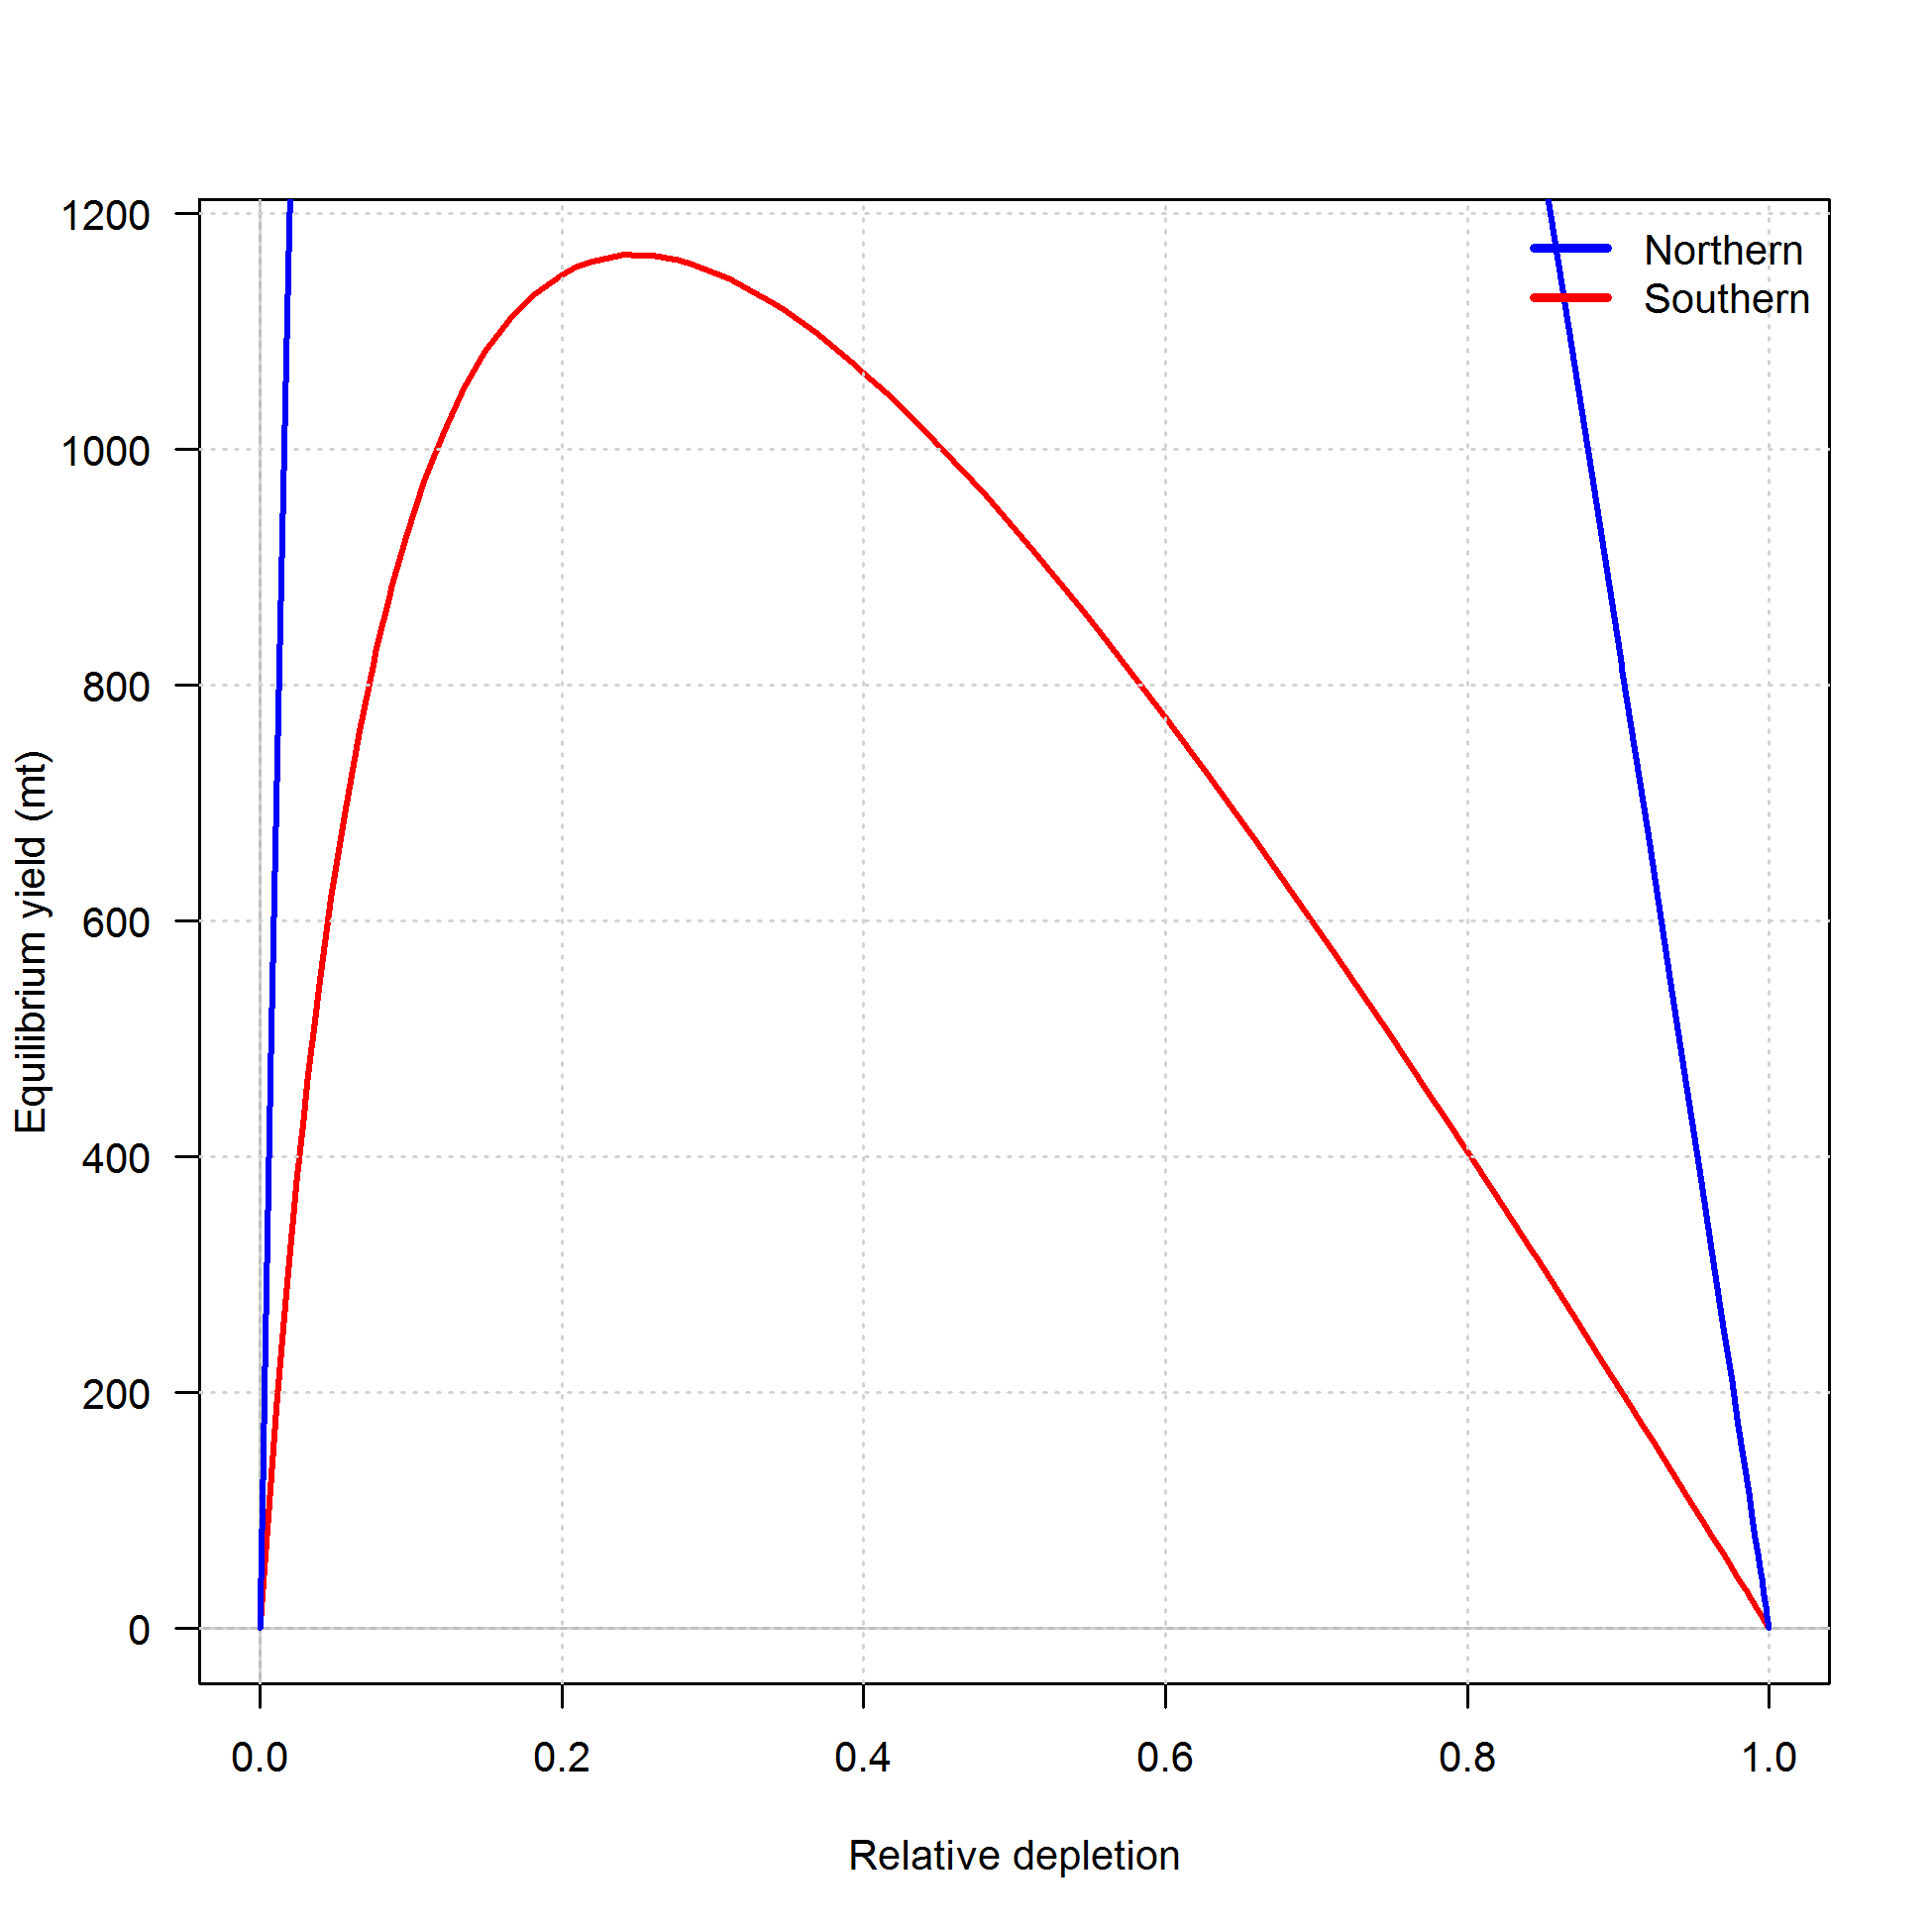
\includegraphics{r4ss/plots_compare/yield_comparison_n_models.png}
\caption{Equilibrium yield curve for the base case
models.\label{fig:Yield_all}}
\end{figure}

\FloatBarrier

\newpage

\subsection*{Research And Data Needs}\label{research-and-data-needs}
\addcontentsline{toc}{subsection}{Research And Data Needs}

\hl{Include: identify information gaps that seriously impede the stock assessment.}

We recommend the following research be conducted before the next
assessment:

\begin{enumerate}

\item List item No. 1 in the list

\item List item No. 2 in the list, etc.

\end{enumerate}

\subsection*{Rebuilding Projections}\label{rebuilding-projections}
\addcontentsline{toc}{subsection}{Rebuilding Projections}

\hl{Include: reference to the principal results from rebuilding analysis if the 
stock is overfished. This section should be included in the Final/SAFE version 
assessment document but is not required for draft assessments undergoing review. 
See Rebuilding Analysis terms of reference for detailed information on 
rebuilding analysis requirements.}

\FloatBarrier

\newpage

\renewcommand{\thefigure}{\arabic{figure}}
\renewcommand{\thetable}{\arabic{table}}

\setcounter{figure}{0} \setcounter{table}{0} \pagenumbering{arabic}

\section{Introduction}\label{introduction}

\subsection{Basic Information}\label{basic-information}

Yellowtail rockfish, \emph{Sebastes flavidus}, occur off the West Coast
of the United States from Baja California to the Aleutian Islands.
Yellowtail is a major commercial species, captured mostly in trawls from
Central California to British Columbia (Love
\protect\hyperlink{ref-Love2011}{2011}). Because it is an aggregating,
midwater species it is usually caught in the commercial midwater trawl
fishery. In California there is a large recreational fishery as well.
The center of yellowtail rockfish abundance is from southern Oregon
through British Columbia (Fraidenburg
\protect\hyperlink{ref-Fraidenburg1980}{1980}).

Once thought to comprise a single stock, a recent genetic study
indicates that there are in fact two sub-species, with a genetic cline
at Cape Mendocino, California, roughly \(40^\circ 10^\prime\) North
Latitude (Hess et al. n.d.). The species has never had a full length and
age integrated assessment south of Cape Mendocino, mainly due to a lack
of fishery-independent data; this assessment represents the first
attempt to do so.

Yellowtail rockfish are colloquially known as ``greenies'', although
\emph{flavidus} is Latin for ``yellow'' (Love
\protect\hyperlink{ref-Love2011}{2011}). We have summarized yellowtail
rockfish life history, fisheries, assessment and management here, but
in-depth, extensive background information on yellowtail and other
managed species is available at (Council
\protect\hyperlink{ref-PFMC2016}{2016}).

\subsection{Map}\label{map}

A map showing the scope of the assessment and depicting boundaries for
fisheries or data collection strata is provided in Figure
\ref{fig:boundary_map}.

\subsection{Life History}\label{life-history}

Rockfish are in general long-lived and slow-growing, however yellowtail
rockfish have a high growth rate relative to other rockfish species,
reaching a maximum size of about 55 cm in approximately 15 years (Tagart
\protect\hyperlink{ref-Tagart1991}{1991}). Yellowtail can live at least
64 years (Love \protect\hyperlink{ref-Love2011}{2011}), however no fish
that old occur in data available for this assessment (For the Northern
model, the 95th percentile of age is 35 years for females and 45 years
for males and for the Southern model, 30 and 40 years respectively for
females and males). Yellowtail rockfish are among those that are
fertilized internally and release live young. Spawning aggregations
occur in the fall, and parturition in the winter and spring
(January-May) (Eldridge et al.
\protect\hyperlink{ref-Eldridge1991}{1991}). Young-of-the-year recruit
to nearshore waters from April through August, migrating to deeper water
in the fall. Preferred habitat is the midwater over reefs and boulder
fields.

Yellowtail rockfish are extremely motile, and make rapid and frequent
ascents and descents of 40 meters; they also exhibit strong homing
tendencies (Love \protect\hyperlink{ref-Love2011}{2011}). They are able
to quickly release gas from their swim bladders, perhaps making them
less susceptible to barotrauma than similar species (Eldridge et al.
\protect\hyperlink{ref-Eldridge1991}{1991}).

Rockfish Conservation Areas (RCAs) have been closed to fishing since
2002. Following that closure, Yellowtail rockfish are among the many
species that have been seen to increase in both abundance and in average
size in Central California (Marks et al.
\protect\hyperlink{ref-Marks2015}{2015}).

Literature values for von Bertallanfy parameters are
\(L_\infty = 52.2, k = 0.17, t_0 = -0.75\) for females,
\(L_\infty = 47.6, k=0.19, t_0 = -1.69\) for males. Length-Weight
parameters are \(W = 0.0287L^{2.822}\) for females,
\(W = 0.0359L^{2.745}\) for males (Love
\protect\hyperlink{ref-Love2011}{2011}). See Section \ref{bio-params}
for a discussion of the new analysis of the weight-length relationship.
Fecundity is represented in the models as: \(1.1185^{-11}W^{4.59}\).
This is a rescaling of the values provided in (Dick et al.
\protect\hyperlink{ref-Dick2017}{2017}).

\subsection{Fishery and Management
History}\label{fishery-and-management-history}

The rockfish fishery off the U.S. Pacific coast first developed off
California in the late 19th century as a hook-and-line fishery (Love et
al. \protect\hyperlink{ref-Love2002}{2002}). The rockfish trawl fishery
was established in the early 1940s, when the United States became
involved in World War II and wartime shortage of red meat created an
increased demand for other sources of protein (Harry and Morgan
\protect\hyperlink{ref-Harry1961}{1961}, Alverson et al.
\protect\hyperlink{ref-Alverson1964}{1964}).

Until late 2002, yellowtail rockfish were harvested as part of a
directed mid-water trawl fishery, with fairly high landings in the 1980s
and 1990s. Yellowtail commonly co-occur with canary, widow rockfish and
several other rockfishes (Tagart
\protect\hyperlink{ref-Tagart1988}{1988}); (Rogers and Pikitch
\protect\hyperlink{ref-Rogers1992}{1992}). Association with these and
other rockfish species has substantially altered fishing opportunity for
yellowtail rockfish since canary rockfish stocks were declared
overfished by National Marine Fisheries service in 2000. In order to
achieve the necessary reduction in the canary rockfish catch, stringent
management measures were adopted, limiting harvest of yellowtail
rockfish as well as other co-occurring species.

Beginning in 2000, shelf rockfish species could no longer be retained by
vessels using bottom trawl footropes with a diameter greater than 8
inches. The use of small footrope gear increases the risk of gear loss
in rocky areas. This restriction was intended to provide an incentive
for fishers to avoid high-relief, rocky habitat, thus reducing the
exposure of many depleted species to trawling. This was reinforced
through reductions in landing limits for most shelf rockfish species.

Since September 2002, Rockfish Conservation Areas (RCAs, areas known to
be critical habitat) have been closed to fishing. Alongside these
closures, limits on landings have been in place that were designed so as
to accommodate incidental bycatch only. These eliminated directed
mid-water fishing opportunities for yellowtail rockfish in non-tribal
trawl fisheries. A somewhat greater opportunity to target yellowtail
rockfish in the trawl fishery has been available since 2011 under the
trawl rationalization program, however quotas for widow and canary
rockfish continue to constrain targeting of yellowtail rockfish. With
the recent improved status of constraining stocks, the industry is
developing strategies to better attain allocations of yellowtail and
widow rockfish.

Yellowtail rockfish are currently managed with stock-specific harvest
specifications north of \(40^\circ 10^\prime\) N. latitude, and as part
of the Southern Shelf Rockfish complex south of \(40^\circ 10^\prime\)
N. latitude. The Over Fishing Limit (OFL) contribution of yellowtail
rockfish to the Southern Shelf Rockfish complex is based on a
data-moderate analysis (Cope et al.
\protect\hyperlink{ref-Cope2013}{2013}).

\subsection{Assessment History}\label{assessment-history}

Early studies of yellowtail stocks on the U.S. West Coast north of
\(40^\circ 10^\prime\) N. latitude (Cape Mendocino, northern California)
began in the 1980s with observational surveys. Statistical assessments
of yellowtail rockfish were conducted in 1982 (Tagart
\protect\hyperlink{ref-Tagart1982}{1982}), 1988 (Tagart
\protect\hyperlink{ref-Tagart1988}{1988}), 1996 (Tagart et al.
\protect\hyperlink{ref-Tagart1997}{1997}), and 1997 (Tagart et al.
\protect\hyperlink{ref-Tagart1997}{1997}) to determine harvest
specifications for the stock. These early assessments employed a variety
of statistical methods, for example, the 1997 assessment used cohort
analysis and dynamic pool modeling. Figure
\ref{fig:assessment_history}shows the timeseries of age 4+ biomass for
Yellowtail Rockfish across past assessments.

The yellowtail assessment in 2000 (Tagart et al.
\protect\hyperlink{ref-Tagart2000}{2000}) was the first that estimated
stock status, with an estimated depletion of 60.5 percent at the start
of 2000. Lai et al. (Lai et al. \protect\hyperlink{ref-Lai2003}{2003})
updated the 2000 assessment and estimated that stock depletion was 46
percent at the start of 2003. A second assessment update was prepared in
2005 (Wallace and Lai \protect\hyperlink{ref-Wallace2005}{2005}) with an
estimated depletion of 55 percent at the start of 2005. The 2000
assessment and updates were age-structured assessments conducted using
AD Model Builder as the software platform for nonlinear optimization
(Fournier et al. \protect\hyperlink{ref-Fournier2012}{2012}).

A data-moderate assessment of yellowtail rockfish south of
\(40^\circ 10^\prime\) N. latitude was conducted in 2013 (Cope et al.
\protect\hyperlink{ref-Cope2013}{2013}). This assessment estimated
depletion at the start of 2013 at 67 percent, and estimated the spawning
biomass at 50,043 mt. This was a large biomass increase relative to
previous estimates and may be attributed to the low removals over the
previous decade.

\hl{Include: Management performance tables comparing 
Overfishing Limit (OFL), Annual Catch Limit (ACL), Harvest Guideline (HG) 
[CPS only], landings, and catch (i.e., landings plus discard) for each area and year.}

Management performance table: (Table \ref{tab:mnmgt_perform})

A summary of these values as well as other base case summary results can
be found in Table \ref{tab:base_summary}.

\subsection{Fisheries off Canada, Alaska, and/or
Mexico}\label{fisheries-off-canada-alaska-andor-mexico}

The 2015 Stock Assessment conducted by the Department of Fisheries and
Oceans (DFO) found the stock to be at 0.49B0, in the ``healthy'' range.

The Alaska Fisheries Science Center assesses yellowtail rockfish as one
of 25 species in the ``Other Rockfish'' complex in the Gulf of Alaska.
The 2015 full assessment of this complex found no evidence of
overfishing, which is confirmed in the 2016 SAFE document(Center
\protect\hyperlink{ref-AFSC2016}{2016}).

Limited catches of yellowtail are reported as far south as Baja
California(Love \protect\hyperlink{ref-Love2011}{2011}).

\newpage

\captionsetup[table]{labelformat=empty,justification=raggedright,font=bf, singlelinecheck=false}

\section{Data}\label{data}

Data used in the Northern and Southern yellowtail rockfish assessments
are summarized in Figures \ref{fig:data_plot} and \ref{fig:data_plot}.

Data sources for the two models are largely distinct. Northern fisheries
and surveys had very sparse data (if any) for the south and vice-versa.
Among the 12 data sources referenced below, only 2 data sources are
common to both models. These are the MRFSS/RecFIN recreational dockside
survey, which focuses on California and Oregon, and the CalCOM
California commercial dataset, which contributed data from the
northern-most California counties (Eureka and Del Norte) to the Northern
model. The CalCOM data account for less than five percent of the
commercial landings in the Northern model, and less than 1\% of the
biological samples.

Commercial landings are not differentiated in either model. For the
Northern model, this is due to the very small portion (1.15 \%) of the
landings that are attributed to non-trawl gear. For the Southern model,
this is due to the paucity of data.

A description of each model's data sources follows.

\subsection{Northern Model Data}\label{northern-model-data}

\vspace{.5cm}

\begin{table}[ht]
\centering
\caption{Summary of the data sources in the Northern model.} 
\label{tab:Data_sources}
\begin{tabular}{lcccccr}
  \hline
Source & Landings & Lengths & Ages & Indices & Discard & Type \\ 
  \hline
PacFIN & Y & Y & Y & Y &  & Commercial \\ 
  WCGOP &  & Y &  &  & Y & Commercial Discards \\ 
  Hake Bycatch & Y & Y & Y & Y &  & Commercial \\ 
  CalCOM & Y & Y & Y &  &  & Commercial \\ 
  WaSport & Y & Y & Y &  &  & Recreational \\ 
  MRFSS & Y & Y &  &  &  & Recreational \\ 
  RecFIN & Y & Y &  &  &  & Recreational \\ 
  Triennial &  & Y & Y & Y &  & Survey \\ 
  NWFSCcombo &  & Y & Y & Y &  & Survey \\ 
  Pikitch &  & Y &  &  & Y & Commercial Study \\ 
  ODFW & Y &  &  &  &  & Historical data \\ 
  WDFW & Y &  &  &  &  & Historical data \\ 
   \hline
\end{tabular}
\end{table}

\subsubsection{Commercial Fishery
Landings}\label{commercial-fishery-landings}

\textbf{Washington and Oregon Landings} The bulk of the commercial
landings for Washington and Oregon came from the from the Pacific
Fisheries Information Network (\textbf{PacFIN}) database.

\textbf{Washington Catch Information}\\
The Washington Department of Fisheries and Wildlife (\textbf{WDFW})
provided historical yellowtail catch for 1889--1980. Landings for
1981-2016 came from the PacFIN database. WDFW also provided catches for
the period 1981 -- 2016 to include the re-distribution of the
unspeciated ``URCK'' landings in PacFIN; this information is currently
not available from PacFIN.

\textbf{Oregon Catch Information}\\
The Oregon Department of Fisheries and Wildlife (\textbf{ODFW}) provided
historical yellowtail catch from 1892-1985. ODFW also provided estimates
of yellowtail rockfish in the in the un-speciated PacFIN ``URCK'' and
``POP1'' catch categories for recent years, and those estimates were
combined with PacFIN landings for 1986-2016.

\textbf{Northern California Catch}\\
The California Commercial Fishery Database (\textbf{CalCOM}) provided
landings for the Northern model for the two counties north of
\(40^\circ 10^\prime\) (Eureka and Del Norte) for 1969-2016.

\textbf{Hake Bycatch}\\
The Alaska Fisheries Science Center (\textbf{AFSC}) provided data for
yellowtail bycatch in the hake fishery from 1976-2016.

\subsubsection{Sport Fishery Removals}\label{sport-fishery-removals}

\textbf{Washington Sport Catch}\\
WDFW provided recreational catches for 1967 and 1975-2016.

\textbf{Oregon Sport Catch}\\
ODFW provided recreational catch data for 1979-2016.

\textbf{MRFSS and RecFIN} Data from Northern California came from the
Marine Recreational Fisheries Statistical Survey (\textbf{MRFSS}) and
from the Recreational Fisheries Information Network (\textbf{RecFIN}).
These are dockside surveys focused on California and Oregon. MRFSS was
conducted from 1980-1989 and 1993-2003, RecFIN from 2004 to the present.

\subsubsection{Estimated Discards}\label{estimated-discards}

\textbf{Commercial Discards}\\
The West Coast Groundfish Observing Program (\textbf{WCGOP}) is an
onboard observer program that has extensively surveyed fishing practices
since 2002, with nearly 100\% observer coverage in the trawl sector in
recent years. WCGOP provided discard ratios for yellowtail rockfish from
2002 to 2015.

\textbf{Pikitch Study}\\
The Pikitch study was conducted between 1985 and 1987 (Pikitch et al.
\protect\hyperlink{ref-Pikitch1988}{1988}). The northern and southern
boundaries of the study were \(48^\circ 42^\prime\) N latitude and
\(42^\circ 60^\prime\) N. latitude respectively, which is primarily
within the Columbia INPFC area (Pikitch et al.
\protect\hyperlink{ref-Pikitch1988}{1988} , Rogers and Pikitch
\protect\hyperlink{ref-Rogers1992}{1992}).

Participation in the study was voluntary and included vessels using
bottom, midwater, and shrimp trawl gears. Observers of normal fishing
operations on commercial vessels collected the data, estimated the total
weight of the catch by tow and recorded the weight of species retained
and discarded in the sample.

Pikitch study discards were aggregated due to small sample size and
included in the data as representing a single year mid-way through the
study.

\subsubsection{Abundance Indices}\label{abundance-indices}

\textbf{Commercial Logbook CPUE}\\
The commercial logbook (fish-ticket) data in PacFIN was used to generate
an index for the years 1987-1998, a period in which management of the
fishery was stable, i.e., regulations weren``t changing fishery
practices.

The data were modeled with a modified Stephens-MacCall approach
(Stephens and MacCall \protect\hyperlink{ref-Stephens2004}{2004}). This
approach uses the species composition of the catch to evaluate the
per-haul probability of encountering a particular species; in this case,
yellowtail rockfish. The intent of the analysis is to eliminate all
hauls from the index that could not encounter yellowtail.

Usually, the Stephens-MacCall approach is a simple binomial model for
presence-absence of the predictive species and the target, however a
generalized linear mixed-effects approach -- modeling the species as
binomial and adding random effects for the interaction of year and
vessel, for haul duration, and for month improved the model fit.

The hauls identified with a reasonable probability of encountering
yellowtail were then modeled in a delta-lognormal glm to produce an
annual index of abundance, bootstrapped 500 times to evaluate
uncertainty.

\textbf{Hake Bycatch Index}

The Hake bycatch data provided by the Alaska Fisheries Science Center
(AFSC) was used to generate an index of abundance for 1985-1999.

Data on haul-by-haul catch of Yellowtail Rockfish and Pacific Hake for
the period 1976-2016 were obtained from the At-Sea Hake Observer Program
along associated information including the location of each tow and the
duration. Previous Yellowtail assessments used an index of abundance for
the years 1978-1999. The most recent assessment (Wallace and Lai, 2005)
stated that the index was not updated to include years beyond 1999
``because subsequent changes in fishery regulations and behavior have
altered the statistical properties of these abundance indices''. The
ending year of 1999 was retained for this analysis. However, the years
up to 1984 have relatively few tows with adequate information for CPUE
analysis, and fishing effort off the coast of Washington where
yellowtail are most commonly encountered (Figure \ref{fig:ASHOP_X1}).
Therefore, for this new analysis, 1985 was chosen as the starting year.

The hake fishery was evolving during the chosen 15 year period
(1985-1999), which included a transition from foreign to domestic fleets
fishing for Pacific Hake (Figure \ref{fig:ASHOP_X2}). The index from the
at-sea hake fishery used in previous assessments standardized for
changes in catchability by using a ratio estimator relating yellowtail
catch to hake catch and then scaling by an estimate of fishing effort
for hake (Equation 1 in Wallace and Lai, 2005). However, that approach
does not take into account differences in the spatial distribution of
the at-sea hake fishery relative to the distributions of hake and
yellowtail.

For this new analysis, changes in catchability were estimated by
comparing an index based on a geostatistical analysis of the hake CPUE
from VAST (Thorson et al. YYYY) to the estimated available hake biomass
from the most recent stock assessment (Berger et al. 2017). The relative
catchability was then used to adjust an independent geostatistical index
of yellowtail CPUE (Figure \ref{fig:ASHOP_X3}). In order to capture the
general trend in catchability, reducing the variability among years,
linear, exponential, and locally smoothed (LOWESS) models were fit to
the time series of individual estimates of hake index to available
biomass (lower panel in Figure \ref{fig:ASHOP_X3}). Of these, the LOWESS
model best captured the pattern of fastest change in the middle of the
time series. The average rate of increase in the resulting estimated
catchability time series is 13\% per year.

VAST was then used to conduct a geostatistical standardization of the
CPUE of yellowtail caught as bycatch in the at-sea hake fishery. The
resulting yellowtail index after adjustment by the estimated changes in
catchability is qualitatively more similar to the index used in previous
assessments (Figure \ref{fig:ASHOP_X4}) than the index resulting from
assuming constant catchability.

\subsubsection{Fishery-Independent Data}\label{fishery-independent-data}

\textbf{Northwest Fisheries Science Center (NWFSC) shelf-slope survey}

This survey, referred to as the \textbf{NWFSCcombo Survey}, has been
conducted annually starting in 2003. It uses a random-grid design
covering the coastal waters from a depth of 55 m to 1,280 m from
late-May to early-October (\hl{add reference: Bradburn 2011}). Four
chartered industry vessels are used each year (with the exception of
2013 when the U.S. federal government shutdown curtailed the survey).

The data from the NWFSCcombo survey was analyzed using a spatio-temporal
delta-model (\hl{add reference: Thorson2015}), implemented as an R
package VAST (\hl{add reference: Thorson2017}) and publicly available
online (\url{https://github.com/James-Thorson/VAST}). Spatial and
spatio-temporal variation is specifically included in both encounter
probability and positive catch rates, a logit-link for encounter
probability, and a log-link for positive catch rates. Vessel-year
effects were included for each unique combination of vessel and year in
the database.

Both lognormal and gamma distributions were explored for the positive
tows and produced similar results with the lognormal model showing
better patterns in Q-Q plot. The index shows variability with an overall
gradual increase from 2003 to 2013 with high estimates near the end of
the time series in 2014 and 2016. A design-based index extrapolated from
swept area densities without any geostatistical standardization shows a
more dramatic increase from 2015 to 2016.

Length and age compositions were also developed from this survey.

\textbf{Alaska Fisheries Science Center (AFSC) Triennial shelf survey}

The \textbf{Triennial Survey} was conducted by the AFSC every third year
between 1977 and 2001, (and was conducted in 2004 by the NWFSC using the
same protocols). The 1977 survey had incomplete coverage and is not
believe to be comparable to the later years. The survey design used
equally-spaced transects from which searches for tows in a specific
depth range were initiated. The depth range and latitudinal range was
not consistent across years, but all years in the period 1980-2004
included the area from 40\(^\circ\) 10'N north to the Canadian border
and a depth range that included 55-366 meters, which spans the range
where the vast majority of Yellowtail encountered in all trawl surveys.
Therefore the index was based on this depth range.

An index of abundance was estimated based on the VAST delta-GLMM model
as described for the NWFSCcombo Index above. In this case as well, Q-Q
plots indicated slightly better performance of the lognormal over gamma
models for positive tows. The index shows a gradual decline from 1980 to
1992 followed by high variability in the final 4 points spanning
1995-2004.

\subsubsection{Biological Samples}\label{biological-samples}

\textbf{Length And Age Compositions}\\
Length composition data were compiled from PacFIN for Oregon and
Washington for the Northern model and combined with raw (unexpanded)
length data from CalCOM for the two California counties north of
40\(^\circ\) 10'N (Eureka and Del Norte counties).

Length compositions were provided from the following sources:

\vspace{.5cm}

\begin{table}[ht]
\centering
\caption{Summary of the time series of lengths used in the stock assessment.} 
\label{tab:Length_sources}
\begin{tabular}{llrrl}
  \hline
Source & Type & Lengths & Tows & Years \\ 
  \hline
PacFIN & commercial & 186161 & 3830 & 1968-2016 \\ 
  CalCOM & commercial & 2340 &  & 1978-2015 \\ 
  MRFSS & recreational & 4125 &  & 1980-2003 \\ 
  RecFIN & recreational & 432 &  & 2004-2016 \\ 
  WASport & recreactional & 11099 &  & 1975-2015 \\ 
  Triennial & survey & 16262 & 465 & 1977-2004 \\ 
  NWFSCcombo & survey & 940 & 564 & 2004-2016 \\ 
   \hline
\end{tabular}
\end{table}

Age structure data were available from the following sources:
\vspace{.5cm}

\begin{table}[ht]
\centering
\caption{Summary of the
                                              time series of age data used in the stock
                                              assessment.} 
\label{tab:Age_sources}
\begin{tabular}{llrrl}
  \hline
Source & Type & Ages & Tows & Years \\ 
  \hline
PacFIN & commercial & 138854 &  & 1972-2016 \\ 
  CalCOM & commercial & 3546 &  & 1980-2002 \\ 
  WASport & recreational & 4027 &  & 1997-2016 \\ 
  Triennial & survey & 6553 & 278 & 1997-2004 \\ 
  NWFSCcombo & survey & 2990 & 544 & 2003-2016 \\ 
   \hline
\end{tabular}
\end{table}

\FloatBarrier
\newpage
\clearpage
\FloatBarrier

\subsection{Southern Model Data}\label{southern-model-data}

\vspace{.5cm}

\begin{table}[ht]
\centering
\caption{Summary of the data source in the Southern model.} 
\label{tab:Data_sources}
\begin{tabular}{lcccccr}
  \hline
Source & Landings & Lengths & Ages & Indices & Discard & Type \\ 
  \hline
CalCOM & Y & Y & Y &  &  & Commercial \\ 
  MRFSS & Y & Y &  &  &  & Recreational \\ 
  RecFIN & Y & Y &  &  &  & Recreational \\ 
  HookandLine &  & Y & Y & Y &  & Survey \\ 
  Onboard &  & Y & Y & Y &  & Survey \\ 
  SmallResearch &  & Y & Y & Y &  & Study \\ 
   \hline
\end{tabular}
\end{table}

\subsubsection{Commercial Fishery
Landings}\label{commercial-fishery-landings-1}

\textbf{California Commercial Landings}\\
The California Commercial Fishery Database (\textbf{CalCOM}) provided
landings in California south of 40\(^\circ\) 10'N for 1969-2016.

\textbf{Historical Data} A reconstruction of the historical commercial
fishery south of Cape Mendocino was provided by the Southwest Fisheries
Science Center (\textbf{SWFSC}) for 1916-1968.

\subsubsection{Sport Fishery Removals}\label{sport-fishery-removals-1}

\textbf{MRFSS Estimates and RecFIN}\\
The California Department of Fish and Wildlife (\textbf{CDFW}) provided
estimated yellowtail removals for the Marine Recreational Fisheries
Statistical Survey (\textbf{MRFSS}) from 1980-1989, 1993-2003. The
Recreational FIsheries Information Network, (\textbf{RecFIN}) provided
landings for 2004-2016.

\textbf{Historical Data} A reconstruction of the historical recreational
fishery south of Cape Mendocino was provided by the Southwest Fisheries
Science Center (\textbf{SWFSC}) for 1928-1980.

\textbf{Small Research Study} A small number of fish were collected from
the recreational fishery by the SWFSC and are included in the data for
1978-1984.

\subsubsection{Estimated Discards}\label{estimated-discards-1}

No discard data were available for the Southern model.

\subsubsection{Abundance Indices}\label{abundance-indices-1}

\textbf{MRFSS Index}\\
An index of abundance was developed from trip-aggregated MRFSS data for
the years 1980-1989, 1992-2003.

\textbf{California Onboard Survey}\\
An Onboard recreational survey conducted by provided data for an index
of abundance provided by the SWFSC for 1987-2016.

\textbf{Research Study Index} An index of abundance for the small
juvenile fish research study was provided by the SWFSC for 2001-2016.

\subsubsection{Fishery-Independent
Data}\label{fishery-independent-data-1}

\textbf{Hook and Line Survey}\\
The NWFSC Hook and Line survey provided data for an index in the
Southern California Bight from 2004-2016.

\subsubsection{Biological Samples}\label{biological-samples-1}

Length composition samples were available for the Southern model from 5
sources, and ages from 3.

Length compositions were provided from the following sources:

\vspace{.5cm}

\begin{table}[ht]
\centering
\caption{Summary of the time series of lengths used in the stock assessment.} 
\label{tab:Length_sources}
\begin{tabular}{llrrl}
  \hline
Source & Type & Lengths & Tows & Years \\ 
  \hline
CalCOM & commercial & 16160 & 1543 & 1978-2015 \\ 
  MRFSS & recreational & 39425 &  & 1980-2003 \\ 
  RecFIN & recreational & 49136 &  & 2004-2016 \\ 
  Onboard & recreational & 76740 &  & 1987-2016 \\ 
  Small Study & recreational & 909 &  & 1978-1984 \\ 
  Hook and Line & survey & 1339 & 174 & 2004-2016 \\ 
   \hline
\end{tabular}
\end{table}

Age structure data were available from the following sources:

\vspace{.5cm}

\begin{table}[ht]
\centering
\caption{Summary of the
                                              time series of age data used in the stock
                                              assessment.} 
\label{tab:Age_sources}
\begin{tabular}{llrl}
  \hline
Source & Type & Ages & Years \\ 
  \hline
CalCOM & commercial & 7875 & 1980-2004 \\ 
  Small Study & recreational & 400 & 1978-1984 \\ 
  Hook and Line & survey & 248 & 2004 \\ 
   \hline
\end{tabular}
\end{table}

\clearpage

\subsection{\texorpdfstring{Biological Parameters Common to Both Models
\label{bio-params}}{Biological Parameters Common to Both Models }}\label{biological-parameters-common-to-both-models}

\vspace{.5cm}

\textbf{Aging Precision And Bias}

Age error matrices were developed for double-reads at the PFMC aging lab
in Newport, OR and for double reads within the WDFW aging lab. The
Newport lab has done all of the Survey aging for the NWFSC, along with
some commercial ages and the 400 fish from the Small Study. WDFW
provided the bulk of recreational and commercial ages. Between-lab
differences in aging were minute, as were within-lab differences. This
result is supported by the primary age reader's assessment: yellowtail
rockfish are extremely easy to age (B. Kamikawa, pers. comm.).

\vspace{.5cm}

\textbf{Weight-Length}

The weight-length relationship is based on the standard power function:
\(W = \alpha(L^\beta)\) where \(W\) is individual weight (kg), \(L\) is
length (cm), and \(\alpha\) and \(\beta\) are coefficients used as
constants.

To estimate this relationship, 12,778 samples with both weight and
length measurements from the fishery independent surveys were analyzed.
These included 6,354 samples from the NWFSC Combo survey, 5,085 from the
Triennial survey, and 1,339 from the Hook and Line survey. All Hook and
Line survey samples were from the Southern area, along with 910 samples
from the other two surveys (Figure \ref{fig:weight-length}).

A single weight-length relationship was chosen for females and males in
both areas after examining various factors that may influence this
relationships, including sex, area, year, and season. None of these
factors had a strong influence in the overall results. Season was one of
the bigger factors, with fish sampled later in the year showing a small
increase in weight at a given length (2-6\% depending on the other
factors considered). However, season was confounded with area because
most of the samples from the Southern area were collected from the Hook
and Line survey which takes place later in the year (mid-September to
mid-November) and the resolution of other data in the model do not
support modeling the stock at a scale finer than a annual time step.

Males and females did not show strong differences in either area, and
the estimated differences were in opposite directions for the two areas,
suggesting that this might be a spurious relationship or confounded with
differences timing of the sampling relative to spawning.

The estimated coefficients resulting from this analysis were
\(\alpha = 1.1843e-05\) and \(\beta = 3.0672\).

\vspace{.5cm}

\textbf{Maturity And Fecundity} Maturity was estimated from histological
analysis of

141 samples collected in 2016. These include 96 from the NWFSC Combo
survey, 25 from mid-water catches in the NWFSC acoustic/trawl survey, 13
from the Hook and Line survey, and 7 from Oregon Department of Fish and
Wildlife. The sample sizes were not adequate to estimate differences in
maturity by area. Length at 50\% maturity was estimated at 42.49cm
(Figure \ref{fig:maturity.png}) which was consistent with the range
37-45cm cited in the previous assessment (Wallace and Lai
\protect\hyperlink{ref-Wallace2005}{2005}).

\vspace{.5cm}

\textbf{Natural Mortality} Natural Mortality priors were provided by
Owen Hamel (pers. comm.). See Section \ref{priors} for further
discussion.

\vspace{.5cm}

\textbf{Sex ratios}

The largest fish seen in the data are females, however the oldest are
males. The sex ratio falls off differently in each model, as can be seen
in Figs(x,y).

\subsubsection{Environmental Or Ecosystem Data Included In The
Assessment}\label{environmental-or-ecosystem-data-included-in-the-assessment}

No environmental index is present in either model.

\newpage

\section{Assessment}\label{assessment}

\subsection{History Of Modeling Approaches Used For This
Stock}\label{history-of-modeling-approaches-used-for-this-stock}

Yellowtail rockfish was previously modeled as an age-structured, 3-area
stock north of \(40^\circ 10^\prime\) in 1999 (Tagart et al.
\protect\hyperlink{ref-Tagart2000}{2000}) using a model written in ADMB
(Fournier et al. \protect\hyperlink{ref-Fournier2012}{2012}); an update
of this assessment was last conducted in 2004 (Wallace and Lai
\protect\hyperlink{ref-Wallace2005}{2005}). That assessment divided the
stock into 3 INPFC areas based on the suggestion that there might be
biological differences in the stock, however recent genetic studies
don't support that (Hess et al. n.d.). The INPFC area boundaries are not
coincident with state boundaries; this is a concern in that recent
reconstructions of historical catch are state-by-state along the West
Coast. Because we cannot produce data that conform to the areas
previously assessed, we have made no effort to reproduce the previous
model.

A data-moderate approach was used to evaluate stock status in 2013 (Cope
et al. \protect\hyperlink{ref-Cope2013}{2013}). The data-moderate model
used only indices of abundance and made simplifying assumptions about
selectivity and growth since no length or age data were included in the
model. This approach is also incompatible with the current model, and we
have made no attempt to reproduce it, either.

\subsubsection{Previous Assessment
Recommendations}\label{previous-assessment-recommendations}

Many of the recommendations of the previous STAR panel are not relevant
to this assessment, as they related to data deficiencies at that time
that have since been resolved. The 2004 STAR particularly recommended a
focus on abundance indices, which they noted might require further
survey information.

This assessment provides four indices for the Northern model, and three
for the Southern model. All indices are newly developed for this
analysis.

\clearpage
\newpage

\subsection{Model Description}\label{model-description}

\subsubsection{Transition To The Current Stock
Assessment}\label{transition-to-the-current-stock-assessment}

These are the main changes from the previous model, and our rationale
for them:

\begin{enumerate}
\def\labelenumi{\arabic{enumi}.}
\item
  Transition to Stock Synthesis. \emph{Rationale}: The Pacific Fishery
  Management Council's preferred modeling platform for stock assessments
  is Stock Synthesis (Methot \protect\hyperlink{ref-Methot2015}{2015}),
  developed since the last full assessment of yellowtail rockfish.
\item
  Addition of Southern model. \emph{Rationale}: Hess, et al. determined
  that the West Coast yellowtail stocks show a genetic cline occurring
  near Cape Mendocino, which is roughly \(40^\circ 10^\prime\) north
  latitude (Hess et al. n.d.). This divides the stock into two
  genetically distinct substocks which we model independently.
\item
  Availability of recent data. \emph{Rationale}: Ten years of data
  collection have occurred since the last update assessment, and the
  data necessary for an assessment of the Southern stock is now
  available.
\item
  Historical catch reconstructions. \emph{Rationale}: Reconstruction of
  catch timeseries in California, Washington and Oregon clarify stock
  history as far back as 1889.
\end{enumerate}

\subsubsection{Definition of Fleets and
Areas}\label{definition-of-fleets-and-areas}

The Northern model comprises the area between Cape Mendocino,
California, and the Canadian border. The Southern model runs from Cape
Mendocino to the Mexican border (Figure \ref{fig:assess_region_map}).

\textbf{Northern Model}

\emph{Commercial}: The commercial fleet consists primarily of bottom and
midwater trawl. No attempt was made to analyze the fishery separately by
gear, particularly since it seems that in the fishery in the 1980s and
1990s, ``bottom trawl'' gear was used in the midwater as well as on the
bottom, and ``midwater gear'' was sometimes dragged across soft bottom
(Craig Goode, ODFW Port Sampler, pers. comm).

The data associated with the commercial fleet includes age- and
length-composition data from PacFIN and CalCOM, historical catch
timeseries from CDFW, ODFW and WDFW. Observations of discards from the
Pikitch research study provide lengths and discard rates; discard
lengths and rates calculated from WCGOP data. Sex was available for the
comps in the retained catch, which is by-sex in the model, but was not
available for the discards, so they are undifferentiated by sex.

The PacFIN logbook (fish ticket) index developed for the commercial
fishery is in fish/tow. Further information about how the data for the
index was worked up is in Appendix \ref{xxx}.

\emph{At-Sea Hake Fishery}: Yellowtail Rockfish are frequently caught in
mid-water trawls associated with the At-Sea Hake Fishery (consisting of
the Catcher-Processor and Mothership sectors). These catches are
recorded and biological sampling takes place but the fish are processed
at sea (typically into fish meal) and are not included in the PacFIN
database, so this fishery requires separate analysis. The At-Sea Hake
fishery provides catches, length compositions by sex, and an index of
abundance.

\emph{Recreational}: The recreational fleet includes data from sport
fisheries off Oregon, and northern California (Eureka and Del Norte
counties), from MRFSS and RecFIN. The index of abundance for the
recreational fleet is in fish per angler-hour. Length data for this
fleet are undifferentiated by sex.

\emph{Washington-Sport}: The Washington data (WA\_Sport) provides
catches, lengths and ages, and was treated as a separate fleet for two
reasons: first, the length composition of the Washington catches were
different from those in the recreational landings in Oregon and northern
California (MRFSS/RecFIN data). There are very large fish in this
dataset, and fewer small ones. Second, the WA\_Sport landings are not
available by weight, so they are entered in the model as numbers,
andStock Synthesis internally converts them to weight using the
combination of estimated selectivity for this fleet (informed by the
length compositions), estimated growth, and the weight-length
relationship. Sex was available for the biological data, however many
lengthed fish were not sexed, so the lengths for this fleet are
undifferentiated by sex, although the ages are.

\emph{Research}: The Alaska Fisheries Science Center's Triennial Trawl
survey, provides age- and length-compositions, and an index of
abundance. This survey was conducted every third year from 1977-2004.
Details on the workup of the CPUE (in biomass/area towed) can be found
in Appendix \ref{xxx}.

The Northwest Fisheries Science Center's NWFSCcombo survey provides age-
and length-compositions, as well as an index of abundance. Details on
the workup of the CPUE (in biomass/area towed) can be found in Appendix
\ref{xxx}.

\emph{Conditional Age-at-Length}: Only the NWFSCcombo ages were used as
conditional age-at-length in the model. All other aged fleets
(Commercial, Washington\_Sport, and Triennial) are present in the model
as marginal ages due to the amount of noise in the age data for those
fleets.

\emph{Indices}: Fish per angler-hour is the basis for the
Washington\_Sport and Pikitch indices. The NWFSCcombo and Triennial
surveys provide indices based on biomass per area-towed. The logbook
survey for the commercial fleet is in units of fish per tow.

\textbf{Southern Model}

\emph{Commercial}: The commercial fleet consists primarily of hook and
line and trawl gear. Hook and line gear account for 78\% of the landings
by weight in the recent period (1978-2016). Commercial data were sexed,
although there are many unsexed lengths. To preserve the large numbers
of lengths, the length data are entered in the model as
undifferentiated, however the ages are sexed and provide the sole
conditional age-at-length timeseries in the Southern Model.

\emph{Recreational}: The recreational fleet includes data from sport
fishery off the California coast south of Cape Mendocino. The
recreational lengths are unsexed. The index is in fish per angler\_hour.
Further information about how the index was worked up is in Appendix
\ref{xxx}.

\emph{California Onbord Recreational Survey}: Research derived-data
include observations from the California Onboard recreational survey.
The length-compositions from this survey are undifferentiated by sex.
The index is in fish per angler\_hour.

\emph{NWFSC Hook-and-Line Survey}: The data from this survey are used in
the model as an index of fish per angler\_hour, a single year of
marginal age data by sex, and sexed length compositions.

\emph{Small Fish Study}: A separate index, length comps and a single
year of ages reflect a small study of juvenile fish conducted by the
SWFSC.

\subsubsection{Modeling Software}\label{modeling-software}

The STAT team used Stock Synthesis 3 (Methot
\protect\hyperlink{ref-Methot2015}{2015}), which is the Pacific Fishery
Management Council's preferred modeling platform for assessments.

\subsubsection{Data Weighting}\label{data-weighting}

Commercial and survey length composition and marginal age composition
data are weighted according to the method of Ian Stewart (pers.comm):

Sample Size = 0.138 * Nfish + Ntows if Nfish/Ntows \textless{} 44, and
Ntows * 7.06 otherwise.

Age-at-Length samples are unwieghted; that is, each fish is assumed to
represent an independent sample.

Recreational trips (the analogue of tows in the commercial fishery) are
difficult to define in most cases. Since much of the recreational data
are from the dockside interview MRFSS program, which didn't anticipate
the need to delineate samples as belonging to particular trips, we chose
to use all recreational data ``as-is'', with the initial weights entered
as number of fish.

Weighting among fleets uses either the Francis method (Francis
\protect\hyperlink{ref-Francis2011}{2011}) or the Ianelli-McAllister
harmonic mean method (McAllister and Ianelli
\protect\hyperlink{ref-McAllister1997}{1997}). The Francis method was
used for all fleets, except for the age data from the Southern model's
Hook and Line survey, which is a single year of data to which we applied
the Ianelli-McAllister method.

\subsubsection{\texorpdfstring{Priors
\label{priors}}{Priors }}\label{priors}

Hamel (Hamel \protect\hyperlink{ref-Hamel2015}{2015}) developed a method
for combining meta-analytic approaches to relating the natural mortality
rate M to other life-history parameters such as longevity, size, growth
rate and reproductive effort, to provide a prior on M. In that same
issue of ICESJMS, Then et al. (Then et al.
\protect\hyperlink{ref-Then2014}{2014}), provided an updated data set of
estimates of M and related life history parameters across a large number
of fish species, from which to develop an M estimator for fish species
in general. They concluded by recommending M estimates be based on
maximum age alone, based on an updated Hoenig non-linear least squares
estimator \(M=4.899A_{max }^{-.916}\).

The approach of basing M priors on maximum age alone was one that was
already being used for west coast rockfish assessments. However, in
fitting the alternative model forms relating M to Amax, Then et al. did
not consistently apply their transformation. In particular, in real
space, one would expect substantial heteroscedasticity in both the
observation and process error associated with the observed relationship
of M to Amax. Therefore, it would be reasonable to fit all models under
a log transformation. This was not done.

Re-evaluating the data used in Then et al. (Then et al.
\protect\hyperlink{ref-Then2014}{2014}) by fitting the one-parameter
Amax model under a log-log transformation (such that the slope is forced
to be -1 in the transformed space (as in Hamel 2015)), the point
estimate for M is \(M=5.4/Amax\)

This is also the median of the prior. The prior is defined as a
lognormal with mean lna(5.4/Amax) and SE = 0.4384343.

Natural mortality priors for these models were based on examination of
the 99\% quantile of the observed ages from early in the time-series,
before the full impact of fishing would have taken place. For the
Northern model, these quantiles were approximately 35 years for females
and 45 years for males, resulting in median M values of 0.15 and 0.12
for females and males. For the Southern model, the 99\% quantile of the
early age observations were approximately 30 and 40 years for females
and males, resulting in median M prior values of 0.18 and 0.135,
respectively. In both models, M for males was represented as an offset
from females. In the Northern model, both the female value and the male
offset could be estimated without priors so the priors were not used.
For the southern model, M was fixed at the median prior values for the
two sexes.

The prior for steepness (\(h\)) assumes a beta distribution with
parameters based on an update of the Thorson-Dorn rockfish prior
(commonly used in past West Coast rockfish assessments) conducted by
James Thorson (personal communication, NWFSC, NOAA) which was reviewed
and endorsed by the Scientific and Statistical Committee in 2017. The
prior is a beta distribution with \(\mu\)=0.718 and \(\sigma\)=0.158.

\subsubsection{General Model
Specifications}\label{general-model-specifications}

Fecundity is represented in the models as: \(1.1185^{-11}W^{4.59}\).
This is a rescaling of the values provided in (Dick et al.
\protect\hyperlink{ref-Dick2017}{2017}).

Model data, control, starter, and forecast files can be found at
\hl{https://DEVORE}

\subsubsection{Estimated And Fixed
Parameters}\label{estimated-and-fixed-parameters}

A full list of all estimated and fixed parameters is provided in
Tables\ldots{}. Estimated and fixed parameters tables currently read in
from .csv file, EXAMPLE: Table \ref{tab:Model1_params}

\textbf{Growth} 5 parameters for female growth are estimated in each
model: 3 von Bertalanffy parameters and 2 parameters for CV as a
function of length at age related to variability in length at age for
small and large fish.

Three parameters are estimated for male growth in each model as offset
from female growth. The size for small fish and CV for small fish were
assumed equal to females.

\textbf{Natural Mortality} Natural mortality is estimated in the
Northern model with an offset for males from females. Natural Mortality
is fixed in the Southern model at the values provided by the Hamel
analysis described above (Hamel
\protect\hyperlink{ref-Hamel2015}{2015}).

\textbf{Selectivity} Selectivity for all fleets was initially estimated
as a 4-parameter double normal, which allows selectivity to be dome
shaped, with parameters controlling the position of the peak
selectivity, the width of the peak, and the ascending and descending
slopes.

For all fleets where the estimated patterns were asymptotic, we fixed
the parameters related to the dome, leaving only the position of the
peak and the ascending slope as estimated parameters. For a few fleets,
the position of the peak hit the upper bound, and was fixed at 55cm.

\textbf{Retention} Retention for commercial fishery in Northern model is
a logistic function of size, with three parameters estimated: length at
50\% retention, the slope of the curve, and the asymptotic retention
fraction. The asymptote was allowed to be time-varying, with one value
applied for the early years through 2001. From 2002 through 2011 we
applied annual time-blocks for theses years when the WCGOP program
observed high discards. The final block runs from 2012 forward,
reflecting the current period in which the implementation of the IFQ
program has led to low discard rates.

\textbf{Other Estimated Parameters} Log(R0) is the equilibrium
recruitment, which is estimated in each model.

Recruitment deviations for the Northern model are estimated from 19xx to
2013. For the Southern model recruitment deviations are estimated from
19xx to 2013.
\hl{list range of years for each model with some comment as to how this range was chosen}.

A parameter for extra standard deviation was added to the index based on
bycatch in the at-sea hake fishery, because this index was not well fit
by any of the models considered.

\clearpage

\subsection{Model Selection and
Evaluation}\label{model-selection-and-evaluation}

\subsubsection{Key Assumptions and Structural
Choices}\label{key-assumptions-and-structural-choices}

Selectivity in both models is asymptotic, with the exception of the
OR-CA MRFSS recreational fleet in the Northern model, and the Onboard
recreational fleet in the Southern model.

For the Northern model, several options for developing a CPUE series for
the recreational fishery were considered but rejected as sparse and
noisy. Similarly, the Washington\_Sport fishery data was evaluated a a
possible source for an index, but the data was not available in a form
useful for a recreational index, i.e., there was no data that provided
for a trip-level analysis of catch and effort, as was used for the MRFSS
index in the Southern model (Stephens and MacCall
\protect\hyperlink{ref-Stephens2004}{2004}).

\subsubsection{Alternate Models
Considered}\label{alternate-models-considered}

Time-blocked selectivity and retention were investigated in the Northern
model, as were domed selectivities.

We also explored time-blocks on selectivity in the Southern model, and
domed selectivity for the MRFSS/RecFIN data.

These approaches resulted in model fits to data that were obviously
poor, and so they were rejected

\subsubsection{Convergence}\label{convergence}

Convergence testing through use of dispersed starting values often
requires extreme values to explore new areas of the multivariate
likelihood surface. Stock Synthesis provides a jitter option that
generates random starting values from a normal distribution logistically
transformed into each parameter's range (Methot
\protect\hyperlink{ref-Methot2015}{2015}). We used this function to find
parameter values for convergence in the Southern model. The Northern
model \hl{report jittering when it's been done}.

\clearpage

\subsection{Response To The Current STAR Panel
Requests}\label{response-to-the-current-star-panel-requests}

\begin{description}[style=unboxed]

\item[Request No. 1: Add after STAR panel.] \hfill \\

    \textbf{Rationale:} Add after STAR panel.  

    \textbf{STAT Response:} Add after STAR panel.

\item[Request No. 2: Add after STAR panel.] \hfill \\

    \textbf{Rationale:} Add after STAR panel.

    \textbf{STAT Response:} Add after STAR panel.

\item[Request No. 3: Add after STAR panel.] \hfill \\

    \textbf{Rationale:} Add after STAR panel.
  
    \textbf{STAT Response:} Add after STAR panel.

\item[Request No. 4: Example of a request that may have a list:] \hfill \\
\begin{itemize}
\item \textbf{Item No. 1}
\item \textbf{Item No. 2}
\item \textbf{Item No. 3, etc.}
\end{itemize}

    \textbf{Rationale:} Add after STAR panel.

    \textbf{STAT Response:} Continue requests as needed.


\end{description}

\clearpage

\subsection{Life History Results for both
models}\label{life-history-results-for-both-models}

Maturity in the model was estimated outside the model at the Northwest
Fisheries Science Center by Melissa Head, and is shown in Figure
\ref{fig:maturity}.

Figure \ref{fig:weight-length} shows the results of the analysis of the
Weight-Length relationship estimated and used as fixed input for both
models.

The growth at the beginning of the year estimated by the models for the
Northern and Southern stocks is shown in Figure \ref{fig:growth}.
Females grow faster in each case, but the Northern stock grows faster
and attains larger maximum size.

\subsection{Northern Model Base Case
Results}\label{northern-model-base-case-results}

The data used in the Northern model by fishery is shown in Figure
\ref{fig:data_plot}. Estimated catches are shown in Figure
\ref{fig:r4ss_total_catch_N}; estimated discards are in Figure
\ref{fig:r4ss_discard_N}. These show the large catches in the 1980s and
90s are being predicted by the model. The large discards in latter years
match the data well for those years.

The timeseries of estimated spawning output in trillions of eggs is
shown in Figure\{fig:ssb\}. The model is estimating two periods of
decline, one beginning in the forties and a steeper decline in the 1970s
and 1980s, followed by an increase since 2000 to pre-1980 levels. There
is a decrease in the final years of the timeseries coincident with
increased uncertainty.

Figure \ref{fig:total_bio} shows the total biomass following a similar
pattern; the ending value is 86069.8 metric tonnes.

The relative spawning output (Figure \ref{fig:depl}) went below the 40\%
target in the early 1980s, and may have been below the minimum stock
size limit of 25\% in the late 1990s, but has rebounded since to
0.567412 (see Table \ref{xxx}).

Figures \ref{fig:recruits1} and \ref{fig:recdevs1} address recruitments
estimated the the model. The first of these shows the age-0 recruits,
and the second the recruitment deviations.
\hl{Ian?  What do we want to say about these?}. The stock-recruit curve,
Figure \ref{fig:stock_recruit_curve} shows a shallow relationship
between stock size and recruitment with
\hl{an asymptote at larger stock sizes.}

\subsubsection{Selectivities, Indices and
Discards}\label{selectivities-indices-and-discards}

Selectivities in the Northern model (Figure \ref{fig:selex}) shows the
difference between the recreational fisheries and the commercial fishery
and survey sampling. All of the fish are fully selected by 50 cm, but
the recreational fish are fully selected at 30 cm.

Retention by length (Figure \ref{fig: retention}) varies over time
between 40\% and 100\%, with no clear pattern of interannual variation,
except for the trawl-rationalization era 2011-present.

Discarding in the commercial fleet (Figure \ref{fig:r4ss_discard_fits})
is fit only by putting blocks on retention in the Northern model.
Discards were very low except during the 1990s and 2000s, until the
trawl-rationalization program implementation.

Fits to the indices for the northern model (Figure \ref{index_fits1})
demonstrate the utility of the NWFSCcombo survey. Although the model
misses the uptick at the end of the timeseries, it is the only recent
index and is well-fit by the model. The other indices are noisier. Most
of the indices are fairly flat, indicating little change in abundance
during each time-period. Although the fit to the Triennial index is
poor, the data nicely reflects the changes in management during it's
tenure: the CPUE was falling during the 1980s and 1990s, then rising
after stringent restrictions began in 2000.

\subsubsection{Lengths}\label{lengths}

Bubble plots for the lengths in the fishery (Figure
\ref{fig:comp_length_bubble_mod1_page1}) show the constancy of the
commercial fleet, and the differences in growth between males and
females; the females are larger, the males smaller. The recreational
fleet is represented by two different sampling regimes, and the
changeover in the mid-2000s is clear in that panel. That the WA\_Sport
fishery catches larger fish is represented in the large bubbles at the
top of the panel. Had we examined that fishery earlier in the process of
putting the model together, we might have settled on a larger maximum
size bin, however that fishery remains the smallest portion of the
catches.

Commercial length comps are very well fit (Figures
\ref{fig:mod1_4_comp_lenfit_data_weighting} and
\ref{fig:mod1_5_comp_lenfit_data_weighting}). Commercial discards are
noiser and not well fit (Figure
\ref{fig:mod1_6_comp_lenfit_data_weighting}). The panel describing the
combined fits and data weighting for the commercial fishery is
duplicted, need to remove redundant figure.

Lengths in the early period of the Hake Bycatch fishery are noisy
(doubtless due to small sample sizes). By 1992, the model is able to fit
the data well (Figure \ref{fig:mod1_10_comp_page1}). Figure
\ref{fig:mod1_13_comp_lenfit_data_weighting} shows that the fits in the
early period have twice (at last) the uncertainty of the later period.

The recreation OR+N.CA timeseries of lengths demonstrates the difference
between the MRFSS sampling and RecFIN sampling. The fits in the early
period are good, those in the later period are noisy and model
uncertainty is high (Figures \ref{fig:mod1_14_comp_l} and \ref{}).

The WA\_Sport length fits might have been improved with a better choice
of maximum size bin for the model (Figures \ref{fig:mod1_18_comp_lenf}
and \ref{fig:mod1_21_comp_lenfit_data_weighting_TA1.8_Recreational}),
however the data are noisy throughout the size range represented.

The Triennial lengths Figures \ref{fig:mod1_22_comp_len} and
\ref{fig:mod1_25_comp_lenfit_data_weighting_TA1.8_Triennial Survey} are
fit well in some years and not in others. The data is not noisy, however
the intermittency of data collection may mean that the model is unable
to capture interannual variation as well as for an annual timeseries.

NWFSCcombo lengths are not well fit, particularly in 2013, where the
data show a large number of small fit that may represent a good
recruitment several years earlier Figures \ref{fig:mod1_26_comp_len} and
\ref{fig:mod1_29_comp_lenfit_data_weighting}.

Figure \ref{fig:mod1_30_comp_lenfit__aggregated_across_time} shows the
relative fits among the data sources, aggregated across time. The
timeseries of presence-absence residuals indicated by filled- and
open-bubbles Figure \ref{fig:comp_Pearson_length_mod1_page1} and Figure
\ref{fig:comp_Pearson_length_mod1_page2} demonstrates the relative
disappointment in model fits; the smaller the bubble, the better the
match between the data and the model expectation.

\subsubsection{Ages}\label{ages}

The NWFSCcombo survey provided the only source of conditional
age-at-length data for the Northern model; ages for other fleets were
treated as marginal ages.

The fits to the marginal commercial Figure \ref{fig:mod1_1_comp} are
quite good from about 1979 on, even fitting the tail where the ages
beyond 55 are lumped. The weightings panel Figure
\ref{fig:mod1_5_comp_agefit_data_weighting_TA1.8_Comme} shows the same
thing: fits are good after about 1979, and the decrease in mean age in
the population corresponds with high catches in the 1980s and 1990s,
with mean age increasing after 2000 as catches were curtailed.

The Washington Sport ages are noisy, and the fit is poor throughout the
timeseries, see Figure \ref{fig:mod1_6_comp_agefit} and Figure
\ref{fig:mod1_9_comp_agefit_data_weighting_TA1.8_Recreational}.

The Triennial ages are noisy but are fit surprisingly well
\ref{fig:mod1_10_comp_agefit};
\ref{fig:mod1_13_comp_agefit_data_weighting_TA1.8_Triennial Survey}.
That the model misses the influx of young fish in 1986 may be due to the
timing of the survey; three-year surveys may not provide enough data for
the model to fit recruitment events.

Aggregated age comps for the Commercial, Washington Sport and Triennial
fleets are shown in Figure
\ref{fig:mod1_14_comp_agefit__aggregated_across_time}, for comparison.
Agreggated fits for the Commercial and Triennial fleets are very
satisfying.

The Ghost age comps Figure \ref{fig:mod1_16_comp} for the NWFSCcombo
survey are the marginal age comps for the survey aggregated over length.
This figure is included for informational purposes only; the marginal
``ghost'' comps are not included in the likelihood calculations. It is
interesting that the model fits this aggregated data poorly, but the
disaggregated data well. This may be due to the fact that for marginal
ages, the data are weighted interannually with number of tows or trips,
but this ghost fleet is unweighted.

Pearson residuals for the marginal age comps, are shown in the bubble
plots in Figure \ref{}. The filled bubbles represent estimates greater
than observations, and the open bubbles observations greater than
estimates. The large filled bubbles at age 25 in a few years suggest
that we might have chosen a slightly older age as the compilation age.

The fits to the length-aggregate NWFSCcombo data show more variation in
mean age in the population in latter years than might be expected in
years with relatively low landings Figure
\ref{fig:mod1_3_comp_condAALfit_data_weighting_TA1.8}. These may
represent young fish recruiting to the fishery, which would happen
approximately 5 years after a biological recruitment event. The
conditional age-at-length fits are shown in Figure
\ref{fig:mod1_4_comp_condAALfit_Andre_plotsflt6mkt2_page1}. These plots
explain the reason this survey was chosen to represent conditional
age-at-length; the model was able to fit these data much better than
other datasets, and improved fit, lower likelihood values and increased
parsimony all contributed to a better model.

\subsection{Northern Model Parameters}\label{northern-model-parameters}

For the Base model, the parameter fits are given in Table
\ref{tab:Model1_params}. Status for all of the estimated parameters is
good, with the exception of the 6th parameter for the selectivity in the
Washington Sport fishery.

\subsubsection{\texorpdfstring{\hl{Northern Model Uncertainty and Sensitivity Analyses}}{}}\label{section}

Table \ref{tab:Sensitivity_model1}

\subsubsection{Northern Model Retrospective
Analysis}\label{northern-model-retrospective-analysis}

\subsubsection{Northern Model Likelihood
Profiles}\label{northern-model-likelihood-profiles}

We profiled the change in negative log likelihood for the data sources
and model total likelihood for critical parameters in the model:
\textbf{R0}, the log of equilibrium recruitment; female natural
mortality, \textbf{MF}; male natural mortality, \textbf{MM}; and
steepness, \textbf{h}, the parameter that reflects how quickly the
stock-recruit relationship allows the stock to rebound from depleted
stock size.

The likelihood profile over a range of values (from 9 to 11) R0 are
shown in Figure \ref{fig:profile_logR0.N}. This plot shows the tension
between the index data and the other data sources. The indices are
better fit with a smaller value of R0, near 9.6, while all other data
sources are better fit at larger values. The overall likelihood in the
model is lowest at 10.3 in this figure. The discards show very little
change (are insensitive) over this range of R0, while the recruitments,
ages and lengths are all minimized at values larger than 10.5.

The likelihood profile over female natural mortality, MF, is over a
range from 0.1 to 0.24 (Figure \ref{fig:profile_M.N}). In this figure,
the indices are fit best when MF is 0.1, the ages and lengths are fit
nearer 0.18, and the recruitments and total log likelihoods are
minimized at 0.15.

Figure \ref{fig:profile_M2.N} shows the likelihood profile for male
natural mortality, MM, over a range of negative values that are the
offset from female mortality (FM). The index data are again at odds with
the other data sources; all but the indices are minimized at a value of
-0.15. Male natural mortality is represented as an offset from that for
females based on the equation \(MM = MF*exp(offset)\), such that an
offset of 0 results in equal mortality for males and females, and an
offset of -0.3 results in a male natural mortality which is about 74\%
of the female mortality (\(exp(-0.3) = 0.7408\)).

The profile over values of steepness, h, from 0.5 to 0.9, Figure
\ref{fig:profile_h.N}, shows the index data for once in the majority as
all data sources except the lengths support 0.9 as minimizing the
likelihood, while the lengths support a value closer to 0.5. The scale
of this plot differs from the others; it is roughly a tenth of the scale
of the R0 plot, meaning that the choice of h within this range has far
less impact on likelihood in the model than choices for the other
profiled parameters. This suggests the stock is not depleted; the choice
of steepness would have a much greater impact on a depleted stock.

\subsubsection{Northern Model Reference
Points}\label{northern-model-reference-points}

Intro sentence or two\ldots{}.(Table \ref{tab:Timeseries_mod1}).

Equilibrium yield at the proxy \(F_{MSY}\) harvest rate corresponding to
\(SPR_{50\%}\) is

\hl{Knit kept whining about missing ref pts table, wouldn't work, took out ref.}

shows the full suite of estimated reference points for the northern area
model and Figure \ref{fig:Yield_all} shows the equilibrium yield curve.

\clearpage

\subsection{Southern Model Base Case
Results}\label{southern-model-base-case-results}

Data used in the Southern model is shown in Figure \ref{fig:data_plot}.

One thing to point out is that although the scale of the biomass in the
model is somewhat sensitive to various data sources, the depletion is
not. In tuning the model we were suprised to note that depletion always
stayed above 80\%.

Estimated catches are shown in Figure \ref{fig:r4ss_catch2_S}.

The estimated spawning biomass in Figure \ref{fig:ssb} shows the size of
the uncertainty in this model. Total biomass (Figure
\ref{fig:total_bio}) shows a sharp upward trend in recent years, the
decade with only one year of age data from the Hook-and-Line Survey.
Spawning depletion has sinuous curves and was likely never as low as the
40\% target, even in the 1980s-1990s (Figure \ref{fig:depl}.

Recruitments have been constant, except 2008 and 2010, when the model
sees extra large recruitments with extra large recruitment deviations
(Figures \ref{fig:recruits1} and \ref{fig:recdevs1}). The
spawner-recruit curve, Figure \ref{fig:stock_recruit_curve} is a line.

\subsubsection{Southern Model Selectivities, Indices and
Discards}\label{southern-model-selectivities-indices-and-discards}

Selectivity by fleet is shown in Figure \ref{fig:selex}. Selectivities
for all but the recreational Onboard fishery are modeled as asymptotic;
both recreational fleets (MRFSS/RecFIN and Onboard) are fully selected
at 30cm; the remaining fleets show full selectivity at 45-50 cm.

Index fits leave something to be desired. All are more-or-less flat,
with all of the three current indices, the Onboard, the Juvenile study
and the Hook-and-Line survey all missing a downturn at the end of the
timeseries. During model tuning, we tried introducing a time-blocked
index for the two periods of the Onboard survey, however it didn't
improve the fit to the index significantly, and increased the (negative
log) likelihood of the model.

There was little information to inform the Southern Model of discard
behavior, except in the Onboard survey, where it was represented by
extremely small numbers. We included these discards in the retained
fishery, since attempts to include it as a type-1 ``retained plus
discards'' fishery prevented the model from converging.

\subsubsection{Southern Model Lengths}\label{southern-model-lengths}

Lengths in the Southern model were entered as unsexed, except for the
Hook-and-Line fishery. There were sexes for the Commercial lengths,
however there were also large numbers of unsexed lengths, and we chose
to model the lengths as unsexed, to include as much of the data as
possible. This was true of the Small-Fish study, as well.

Bubble plots of the lengths by year in each fishery are in Figure
\ref{fig:comp_length_bubble_mod2}. The plot for the recreational fishery
clearly shows the transition from the MRFSS sampling program to RecFIN
in 2003/2004, as well as suggesting the existence of larger fish in the
1980s. The Commercial fishery data has been sparse in recent years,
however the fish taken in the Commercial catch are consistently larger
than those in the recreational fishery, no doubt reflecting trawling in
deeper waters. The Onboard survey lengths reflect two eras of sampling,
again with larger fish in the earlier period. The panel for the
Hook-and-Line survey shows that the females landed are always larger
than the males, in agreement with the model estimates of growth: Figure
\ref{fig:growth}.

The fits to the lengths in the Recreational fishery Figure
\ref{fig:mod2_1_comp_len} show variable fits through the years, with the
noisy and sparse data in 2004 heralding the transition between MRFSS
sampling and RecFIN. Overall, the timeseries is fit fairly well: Figure
\ref{fig:mod2_4_comp_lenfit_data_weighting_}

The Commercial length comps are fit well through 2005, when data becomes
sparse and noisy Figure \ref{fig:mod2_5_comp_len}; and Figure
\ref{fig:mod2_8_comp_lenfit_data_weighting_T}.

Fits for the Onboard Survey lengths are good in the early survey, and
poor for the later period \ref{fig:mod2_9_comp}; \ref{fig:mod2_12_comp}.
Attempting to apply a time-block to this data resulted in poor
convergence.

The Hook-and-Line Survey lengths are noisy (Figure
\ref{fig:mod2_13_comp_l}), but the fits are acceptable, and follow the
trend of the data better than those for the other datasets: Figure
\ref{fig:mod2_16_comp_lenfit_data_weighting}.

The small fish survey lengths are not fit badly
\ref{fig:mod2_17_comp_len};
\ref{fig:mod2_20_comp_lenfit_data_weighting}, and it is perhaps a shame
that there are so few years to this timeseries.

The aggregate fits to the length comps for all five datasets is shown in
Figure \ref{fig:mod2_21_comp_lenfit__aggregated_across_time}, and
Pearson residuals for the lengths in Figure
\ref{fig:comp_Pearson_length_mod2}. Filled bubbles represent
under-estimation of the data, open bubbles represent overestimation.

\subsubsection{Southern Model Ages}\label{southern-model-ages}

There are few marginal ages in the model. Bubble plots for the Southern
model ages (Figure \ref{comp_age_bubble_mod2}) show the small sample
from the Juvenile Fish Study and the single year of ages from the
Hook-and-Line Survey. The samples are too small to show any inter-annual
variation, and are noisy within-year.

Figure \ref{fig:mod2_1_comp_agefits} shows the fit to the Juvenile Fish
samples, which is poor in all four years. The mean age in this data is
shown in Figure
\ref{fig:mod2_4_comp_agefit_data_weighting_TA1.8_Recreational}, at 10
years.

The Hook-and-Line Survey age ``fit'' is shown in Figure
\ref{fig:mod2_5_comp_agefit}. Mean age could not be calculated for the
single year of data, as it is a inter-annual mean.

The aggregated fits for the marginal, and I \emph{do} mean
\emph{marginal} ages are shown in Figure
\ref{fig:mod2_9_comp_agefit__aggregated_across_time}. They speak for
themselves.

The ghost fleet commercial comps aggregated as a marginal timeseries is
shown in Figure \ref{fig:mod2_11_comp_ghost}. This figure is included
for informational purposes only; ghosts do not contribute to the model
likelihood calculations. The fits here are quite good 1981-1999, however
the last three years of data are very sparse and not well fit.

Pearson residuals for the Small Fish Juvenile Study and the
Hook-and-Line Survey are shown in Figure
\ref{fig:comp_Pearson_age_mod2}. Bubble size indicates the amount of
disappointment in the fits. The filled bubbles indicate underestimates
by the model; the open bubbles indicate overestimates.

The good news age-data comes from the commercial fleet, as was
foreshadowed by the ghost fleet. Figure
\ref{fig:mod2_4_comp_condAALfit_data_weighting_TA1.8_condAgeCommercial}
shows the interannual fits to the mean age in the commercial
age-at-length data. Except for 1981, 1982 and 1989, the model is able to
fit the data reasonably well, detecting the downward trend in the late
1980s and into the mid-1990s.

The annual plots of age-at-length fits (Figure
\ref{fig:mod2_5_comp_condAALfit_Andre_plotsflt2mkt2_page1}) show good
fits in all years except 2001-2002 (``the sparse years, when we had to
eat Gefilte-miltz'').

\subsubsection{Southern Model Uncertainty and Sensitivity
Analyses}\label{southern-model-uncertainty-and-sensitivity-analyses}

\subsubsection{Southern Model Retrospective
Analysis}\label{southern-model-retrospective-analysis}

\subsubsection{Southern Model Likelihood
Profiles}\label{southern-model-likelihood-profiles}

We profiled the change in negative log likelihood for the data sources
and model total likelihood for critical parameters fixed in the model:
\textbf{R0}, the log of equilibrium recruitment; female natural
mortality, \textbf{MF}; male natural mortality, \textbf{MM}; and
steepness, \textbf{h} the parameter that reflects how quickly the
stock-recruit relationship allows the stock to rebound from depleted
stock size.

The likelihood profile for \textbf{R0} is shown in Figure
\ref{fig:profile_logR0.S}. R0 was profiled over values from 8.5 -11. The
figure shows that the age data and indices are minimized when R0 is 11;
the length data are minimized around 8.5, and the recruitments at 9.8
(or so). The overall likelihood is minimized near 10.5.

The female natural mortality (FM) profile, \ref{fig:profile_M.S} ranges
from 0.1 to 0.24. The age and length data sources are at odds over FM;
the ages and recruitments are minimized when FM is the low end of the
range, and the lengths and indices when it is highest. Changes to the
recruitment likelihood is minimal over the whole range. The overall
likelihood is minimized near 0.22.

Male natural mortality (MM) is profiled over a range from -0.4 to 0.
Male natural mortality is represented as an offset from that for females
based on the equation \(MM = MF*exp(offset)\), such that an offset of 0
results in equal mortality for males and females, and an offset of -0.3
results in a male natural mortality which is about 74\% of the female
mortality (\(exp(-0.3) = 0.7408\)). All roads lead to Rome in this
figure (Figure \ref{fig:profile_M2.S}); since all data sources and the
overall likelihood are minimized at zero. Likelihoods for recruitments
and indices are flat over the range of MM; the other data sources show
changes of 20 (lengths) and 80 (ages) likelihood values.

The steepness profile (Figure \ref{fig:profile_h.S}is the most colorful,
as the lines bounce around and change direction, however the likelihood
scale is from 0 to 0.7, meaning that none of the values in this range
(0.5 - 0.9) would have much impact on likelihood in the model. This
supports the conclusion that the stock is abundant. For a depleted
stock, steepness would have a very large impact on the likelihood.

\subsubsection{Southern Model Reference
Points}\label{southern-model-reference-points}

\subsection{Comparison of the Northern and Southern Model
Results.}\label{comparison-of-the-northern-and-southern-model-results.}

\hl{No text yet}

\newpage

\section{Harvest Projections and Decision
Tables}\label{harvest-projections-and-decision-tables}

Table \ref{tab:mnmgt_perform}

** Northern Model Projections and Decision Table (groundfish only)**
(Table \ref{tab:Forecast_mod1}

Table \ref{tab:Decision_table_mod1}

** Southern Model Projections and Decision Table (groundfish only)**

\newpage

\section{Regional Management
Considerations}\label{regional-management-considerations}

Management of the yellowtail rockfish northern stock has always been
delineated by the 40\(^\circ\) 10' line and the Canadian border. That
the stock's genetic cline was found at Cape Mendocino is a happy
accident that reinforces 40\(^\circ\) 10' as the appropriate management
line.

This assessment was not designed to test that choice. Given that the
data for commercial and recreational fisheries is collected by the
individual states (WA, OR, CA), it might have been interesting to
investigate a management line at the California/Oregon border, had the
STAT team the time and managers the interest in investigating a change.

\newpage

\section{Research Needs}\label{research-needs}

\begin{enumerate}

\item A longer timeseries of the juvenile rockfish CPUE in the south.

\item A commercial index in the north.  This is by far the largest segment of the fishery, and the introduction of trawl rationalization program should mean that an index can be developed for the current fishery when the next assessment is performed.

\item More recent ages for the southern model.  The commercial age timeseries currently stops in 2002.

\end{enumerate}

\newpage

\section{Acknowledgments}\label{acknowledgments}

The authors thank the following individuals for their contributions to
this assessment:

Washington Department of Fish and Wildlife staff: Theresa Tsou and
Phillip Weyland

Oregon Department of Fish and Wildlife staff: Alison Whitman and Troy
Buell

California Department of Fish and Wildlife staff: John Budrick

Southwest Fisheries Science Center staff: Melissa Monk, E.J. Dick, and
Don Pearson

Northwest Fisheries Science Center staff: Jim Hastie, Chantel Wetzel,
Beth Horness, Melissa Head, John Wallace, Vanessa Tuttle, James Thorson
and Owen Hamel

RecFIN staff: Rob Ames

John DeVore, Pacific Fisheries Management Council staff

John Field, STAR panel Chair, SWFSC

CIE Reviewers: Panagiota Apostolaki and Kevin Stokes

John Budrick, CDFW

Jessi Doerpinghaus, WDFW and Pacific Fishery Management Council /
Groundfish Management Team

Dan Waldeck, Pacific Fishery Management Council / Groundfish Advisory
Panel

\newpage

\renewcommand{\thefigure}{\arabic{figure}}
\renewcommand{\thetable}{\arabic{table}}

\setcounter{figure}{0} \setcounter{table}{0} \newpage

\captionsetup[table]{labelformat=simple,format=plain,labelsep=period}

\section{Tables}\label{tables}

\begin{table}[ht]
\centering
\caption{Summary of the biomass/abundance
                                              time series used in the stock
                                              assessment.} 
\label{tab:Index_summary}
\begin{tabular}{>{\centering}p{.4in}>{\centering}p{.3in}>{\centering}p{.3in}>{\centering}p{.3in}>{\centering}p{.6in}>{\centering}p{.5in}>{\centering}p{.8in}>{\centering}p{.8in}>{\centering}p{.5in}}
  \hline
Region & ID & Fleet & Years & Name & Fishery ind. & Filtering & Method & Endorsed \\ 
  \hline
WA & 1 & 4 & 1981-2014 & Dockside CPUE & No & trip, area, month, Stephens-MacCall & delta-GLM (bin-gamma) & SSC \\ 
  - & - & - & - & - & - & - & - & - \\ 
  - & - & - & - & - & - & - & - & - \\ 
  - & - & - & - & - & - & - & - & - \\ 
   \hline
\end{tabular}
\end{table}

\newpage

\begin{table}[ht]
\centering
\caption{Results from 100 jitters from each of 
                                      the three models.} 
\label{tab:jitter}
\begin{tabular}{llll}
  \hline
Status & Model.1 & Model.2 & Model.3 \\ 
  \hline
Returned to base case & - & - & - \\ 
  Found local minimum & - & - & - \\ 
  Found better solution & - & - & - \\ 
  Error in likelihood & - & - & - \\ 
  Total & 100 & 100 & 100 \\ 
   \hline
\end{tabular}
\end{table}

\FloatBarrier

\begin{landscape}
\begin{longtable}{rlrrcccl}
\caption{List of parameters used in
                                              the base model, including estimated 
                                              values and standard deviations (SD), 
                                              bounds (minimum and maximum), 
                                              estimation phase (negative values indicate
                                              not estimated), status (indicates if 
                                              parameters are near bounds, and prior type
                                              information (mean, SD).} \\ 
  \hline
No. & Parameter & Value & Phase & Bounds & Status & SD & Prior (Exp.Val, SD)  \\ 
  \hline 
\endhead 
\hline 
\multicolumn{3}{l}{\footnotesize Continued on next page} 
\endfoot 
\endlastfoot 
 \hline
1 & NatM\_p\_1\_Fem\_GP\_1 & 0.149 & 2 & (0.02, 0.25) & OK & 0.009 & None \\ 
  2 & L\_at\_Amin\_Fem\_GP\_1 & 15.094 & 3 & (1, 25) & OK & 0.556 & None \\ 
  3 & L\_at\_Amax\_Fem\_GP\_1 & 53.899 & 2 & (35, 70) & OK & 0.238 & None \\ 
  4 & VonBert\_K\_Fem\_GP\_1 & 0.135 & 3 & (0.1, 0.4) & OK & 0.004 & None \\ 
  5 & CV\_young\_Fem\_GP\_1 & 0.098 & 5 & (0.03, 0.16) & OK & 0.010 & None \\ 
  6 & CV\_old\_Fem\_GP\_1 & 0.044 & 5 & (0.03, 0.16) & OK & 0.003 & None \\ 
  7 & Wtlen\_1\_Fem & 0.000 & -50 & (0, 3) &  &  & None \\ 
  8 & Wtlen\_2\_Fem & 3.067 & -50 & (2, 4) &  &  & None \\ 
  9 & Mat50\%\_Fem & 42.490 & -50 & (30, 56) &  &  & None \\ 
  10 & Mat\_slope\_Fem & -0.401 & -50 & (-2, 1) &  &  & None \\ 
  11 & Eggs\_scalar\_Fem & 0.000 & -50 & (0, 6) &  &  & None \\ 
  12 & Eggs\_exp\_len\_Fem & 4.590 & -50 & (2, 7) &  &  & None \\ 
  13 & NatM\_p\_1\_Mal\_GP\_1 & -0.142 & 2 & (-3, 3) & OK & 0.016 & None \\ 
  14 & L\_at\_Amin\_Mal\_GP\_1 & 0.000 & -2 & (-1, 1) &  &  & None \\ 
  15 & L\_at\_Amax\_Mal\_GP\_1 & -0.150 & 2 & (-1, 1) & OK & 0.005 & None \\ 
  16 & VonBert\_K\_Mal\_GP\_1 & 0.381 & 3 & (-1, 1) & OK & 0.027 & None \\ 
  17 & CV\_young\_Mal\_GP\_1 & 0.000 & -5 & (-1, 1) &  &  & None \\ 
  18 & CV\_old\_Mal\_GP\_1 & 0.168 & 5 & (-1, 1) & OK & 0.070 & None \\ 
  19 & Wtlen\_1\_Mal & 0.000 & -50 & (0, 3) &  &  & None \\ 
  20 & Wtlen\_2\_Mal & 3.067 & -50 & (2, 4) &  &  & None \\ 
  24 & CohortGrowDev & 1.000 & -50 & (0, 2) &  &  & None \\ 
  25 & FracFemale\_GP\_1 & 0.500 & -99 & (0.001, 0.999) &  &  & None \\ 
  26 & SR\_LN(R0) & 10.320 & 1 & (5, 20) & OK & 0.154 & None \\ 
  27 & SR\_BH\_steep & 0.718 & -6 & (0.2, 1) &  &  & None \\ 
  28 & SR\_sigmaR & 0.546 & -6 & (0.5, 1.2) &  &  & None \\ 
  29 & SR\_regime & 0.000 & -50 & (-5, 5) &  &  & None \\ 
  30 & SR\_autocorr & 0.000 & -50 & (0, 2) &  &  & None \\ 
  140 & LnQ\_base\_CommercialTrawl(1) & -4.443 & -1 & (-30, 15) &  &  & None \\ 
  141 & LnQ\_base\_HakeByCatch(2) & -9.851 & -1 & (-30, 15) &  &  & None \\ 
  142 & Q\_extraSD\_HakeByCatch(2) & 0.297 & 1 & (0, 0.5) & OK & 0.086 & None \\ 
  143 & LnQ\_base\_Triennial(5) & -1.004 & -1 & (-30, 15) &  &  & None \\ 
  144 & LnQ\_base\_NWFSCcombo(6) & -0.616 & -1 & (-30, 15) &  &  & None \\ 
  145 & SizeSel\_P1\_CommercialTrawl(1) & 48.832 & 1 & (20, 55) & OK & 0.701 & None \\ 
  146 & SizeSel\_P2\_CommercialTrawl(1) & 70.000 & -4 & (-20, 70) &  &  & None \\ 
  147 & SizeSel\_P3\_CommercialTrawl(1) & 4.286 & 3 & (-5, 20) & OK & 0.092 & None \\ 
  148 & SizeSel\_P4\_CommercialTrawl(1) & 70.000 & -4 & (-5, 70) &  &  & None \\ 
  149 & SizeSel\_P5\_CommercialTrawl(1) & -999.000 & -99 & (-999, 25) &  &  & None \\ 
  150 & SizeSel\_P6\_CommercialTrawl(1) & -999.000 & -99 & (-999, 25) &  &  & None \\ 
  151 & Retain\_P1\_CommercialTrawl(1) & 24.650 & 3 & (20, 55) & OK & 3.300 & None \\ 
  152 & Retain\_P2\_CommercialTrawl(1) & 1.582 & 3 & (0.1, 40) & OK & 0.708 & None \\ 
  153 & Retain\_P3\_CommercialTrawl(1) & 3.071 & 3 & (-10, 20) & OK & 0.708 & None \\ 
  154 & Retain\_P4\_CommercialTrawl(1) & 0.000 & -4 & (-3, 3) &  &  & None \\ 
  155 & SizeSel\_P1\_HakeByCatch(2) & 52.344 & 1 & (20, 55) & OK & 0.859 & None \\ 
  156 & SizeSel\_P2\_HakeByCatch(2) & 70.000 & -4 & (-20, 70) &  &  & None \\ 
  157 & SizeSel\_P3\_HakeByCatch(2) & 4.281 & 3 & (-5, 20) & OK & 0.111 & None \\ 
  158 & SizeSel\_P4\_HakeByCatch(2) & 70.000 & -4 & (-5, 70) &  &  & None \\ 
  159 & SizeSel\_P5\_HakeByCatch(2) & -999.000 & -99 & (-999, 25) &  &  & None \\ 
  160 & SizeSel\_P6\_HakeByCatch(2) & -999.000 & -99 & (-999, 25) &  &  & None \\ 
  161 & SizeSel\_P1\_RecORandCA(3) & 30.553 & 1 & (20, 55) & OK & 0.698 & None \\ 
  162 & SizeSel\_P2\_RecORandCA(3) & 4.047 & 4 & (-20, 7) & OK & 9229.460 & None \\ 
  163 & SizeSel\_P3\_RecORandCA(3) & 3.132 & 3 & (-5, 20) & OK & 0.230 & None \\ 
  164 & SizeSel\_P4\_RecORandCA(3) & 9.475 & 4 & (-5, 20) & OK & 17038.000 & None \\ 
  165 & SizeSel\_P5\_RecORandCA(3) & -999.000 & -99 & (-999, 25) &  &  & None \\ 
  166 & SizeSel\_P6\_RecORandCA(3) & -999.000 & -99 & (-999, 25) &  &  & None \\ 
  167 & SizeSel\_P1\_RecWA(4) & 28.338 & 6 & (20, 55) & OK & 0.919 & None \\ 
  168 & SizeSel\_P2\_RecWA(4) & 70.000 & -4 & (-20, 70) &  &  & None \\ 
  169 & SizeSel\_P3\_RecWA(4) & -1.427 & 6 & (-5, 20) & OK & 2.392 & None \\ 
  170 & SizeSel\_P4\_RecWA(4) & 70.000 & -4 & (-5, 70) &  &  & None \\ 
  171 & SizeSel\_P5\_RecWA(4) & -999.000 & -99 & (-999, 25) &  &  & None \\ 
  172 & SizeSel\_P6\_RecWA(4) & -999.000 & -99 & (-999, 25) &  &  & None \\ 
  173 & SizeSel\_P1\_Triennial(5) & 54.793 & 1 & (20, 55) & HI & 4.207 & None \\ 
  174 & SizeSel\_P2\_Triennial(5) & 70.000 & -4 & (-20, 70) &  &  & None \\ 
  175 & SizeSel\_P3\_Triennial(5) & 5.127 & 3 & (-5, 20) & OK & 0.316 & None \\ 
  176 & SizeSel\_P4\_Triennial(5) & 70.000 & -4 & (-5, 70) &  &  & None \\ 
  177 & SizeSel\_P5\_Triennial(5) & -999.000 & -99 & (-999, 25) &  &  & None \\ 
  178 & SizeSel\_P6\_Triennial(5) & -999.000 & -99 & (-999, 25) &  &  & None \\ 
  179 & SizeSel\_P1\_NWFSCcombo(6) & 49.892 & 1 & (20, 55) & OK & 2.853 & None \\ 
  180 & SizeSel\_P2\_NWFSCcombo(6) & 70.000 & -4 & (-20, 70) &  &  & None \\ 
  181 & SizeSel\_P3\_NWFSCcombo(6) & 4.544 & 3 & (-5, 20) & OK & 0.419 & None \\ 
  182 & SizeSel\_P4\_NWFSCcombo(6) & 70.000 & -4 & (-5, 70) &  &  & None \\ 
  183 & SizeSel\_P5\_NWFSCcombo(6) & -999.000 & -99 & (-999, 25) &  &  & None \\ 
  184 & SizeSel\_P6\_NWFSCcombo(6) & -999.000 & -99 & (-999, 25) &  &  & None \\ 
  185 & Retain\_P3\_CommercialTrawl(1)\_BLK1repl\_2002 & 2.228 & 6 & (-10, 20) & OK & 0.457 & None \\ 
  186 & Retain\_P3\_CommercialTrawl(1)\_BLK1repl\_2003 & 3.708 & 6 & (-10, 20) & OK & 0.756 & None \\ 
  187 & Retain\_P3\_CommercialTrawl(1)\_BLK1repl\_2004 & 1.129 & 6 & (-10, 20) & OK & 0.522 & None \\ 
  188 & Retain\_P3\_CommercialTrawl(1)\_BLK1repl\_2005 & -0.112 & 6 & (-10, 20) & OK & 0.400 & None \\ 
  189 & Retain\_P3\_CommercialTrawl(1)\_BLK1repl\_2006 & 1.760 & 6 & (-10, 20) & OK & 0.260 & None \\ 
  190 & Retain\_P3\_CommercialTrawl(1)\_BLK1repl\_2007 & -0.514 & 6 & (-10, 20) & OK & 0.623 & None \\ 
  191 & Retain\_P3\_CommercialTrawl(1)\_BLK1repl\_2008 & 2.370 & 6 & (-10, 20) & OK & 0.815 & None \\ 
  192 & Retain\_P3\_CommercialTrawl(1)\_BLK1repl\_2009 & 0.481 & 6 & (-10, 20) & OK & 0.495 & None \\ 
  193 & Retain\_P3\_CommercialTrawl(1)\_BLK1repl\_2010 & 0.161 & 6 & (-10, 20) & OK & 0.677 & None \\ 
  194 & Retain\_P3\_CommercialTrawl(1)\_BLK1repl\_2011 & 7.316 & 6 & (-10, 20) & OK & 0.661 & None \\ 
   \hline
\hline
\label{tab:model_params}
\end{longtable}
\end{landscape}

\newpage

\begin{sidewaystable}[ht]
\centering
\caption{Sensitivity of the base model 
                                          to dropping or down-weighting data 
                                          sources and alternative assumptions 
                                          about growth.} 
\label{tab:Sensitivity_model1}
\scalebox{0.9}{
\begin{tabular}{l>{\centering}p{.6in}>{\centering}p{.6in}>{\centering}p{.6in}>{\centering}p{.6in}>{\centering}p{.6in}>{\centering}p{.6in}>{\centering}p{.6in}>{\centering}p{.6in}}
  \hline
Label & Base (Francis weights) & Harmonic mean weights & Drop index & Drop ages & Down-weight lengths & Free size Age0 & Free CV Amin & External growth \\ 
  \hline
TOTAL\_like & - & - & - & - & - & - & - & - \\ 
  Catch\_like & - & - & - & - & - & - & - & - \\ 
  Equil\_catch\_like & - & - & - & - & - & - & - & - \\ 
  Survey\_like & - & - & - & - & - & - & - & - \\ 
  Length\_comp\_like & - & - & - & - & - & - & - & - \\ 
  Age\_comp\_like & - & - & - & - & - & - & - & - \\ 
  Parm\_priors\_like & - & - & - & - & - & - & - & - \\ 
  SSB\_Unfished\_thousand\_mt & - & - & - & - & - & - & - & - \\ 
  TotBio\_Unfished & - & - & - & - & - & - & - & - \\ 
  SmryBio\_Unfished & - & - & - & - & - & - & - & - \\ 
  Recr\_Unfished\_billions & - & - & - & - & - & - & - & - \\ 
  SSB\_Btgt\_thousand\_mt & - & - & - & - & - & - & - & - \\ 
  SPR\_Btgt & - & - & - & - & - & - & - & - \\ 
  Fstd\_Btgt & - & - & - & - & - & - & - & - \\ 
  TotYield\_Btgt\_thousand\_mt & - & - & - & - & - & - & - & - \\ 
  SSB\_SPRtgt\_thousand\_mt & - & - & - & - & - & - & - & - \\ 
  Fstd\_SPRtgt & - & - & - & - & - & - & - & - \\ 
  TotYield\_SPRtgt\_thousand\_mt & - & - & - & - & - & - & - & - \\ 
  SSB\_MSY\_thousand\_mt & - & - & - & - & - & - & - & - \\ 
  SPR\_MSY & - & - & - & - & - & - & - & - \\ 
  Fstd\_MSY & - & - & - & - & - & - & - & - \\ 
  TotYield\_MSY\_thousand\_mt & - & - & - & - & - & - & - & - \\ 
  RetYield\_MSY & - & - & - & - & - & - & - & - \\ 
  Bratio\_2015 & - & - & - & - & - & - & - & - \\ 
  F\_2015 & - & - & - & - & - & - & - & - \\ 
  SPRratio\_2015 & - & - & - & - & - & - & - & - \\ 
  Recr\_2015 & - & - & - & - & - & - & - & - \\ 
  Recr\_Virgin\_billions & - & - & - & - & - & - & - & - \\ 
  L\_at\_Amin\_Fem\_GP\_1 & - & - & - & - & - & - & - & - \\ 
  L\_at\_Amax\_Fem\_GP\_1 & - & - & - & - & - & - & - & - \\ 
  VonBert\_K\_Fem\_GP\_1 & - & - & - & - & - & - & - & - \\ 
  CV\_young\_Fem\_GP\_1 & - & - & - & - & - & - & - & - \\ 
  CV\_old\_Fem\_GP\_1 & - & - & - & - & - & - & - & - \\ 
   \hline
\end{tabular}
}
\end{sidewaystable}

\newpage

\begin{longtable}{c>{\centering}p{.6in}>{\centering}p{.6in}>{\centering}p{.6in}>{\centering}p{.6in}>{\centering}p{.8in}>{\centering}p{.8in}c}
\caption{Time-series of population estimates 
                                        from the base-case model.} \\ 
  \hline
Yr & Total biomass (mt) & Spawning biomass (mt) & Depletion & Age-0 recruits & Total catch (mt) & Relative exploitation rate & SPR \\ 
  \hline \endhead  \hline
1889 & 132737 & 14 & 0.00 & 30370 & 0 & 0.00 & 1.00 \\ 
  1890 & 132737 & 14 & 1.00 & 30370 & 0 & 0.00 & 1.00 \\ 
  1891 & 132736 & 14 & 1.00 & 30370 & 0 & 0.00 & 1.00 \\ 
  1892 & 132718 & 14 & 1.00 & 30370 & 2 & 0.00 & 1.00 \\ 
  1893 & 132721 & 14 & 1.00 & 30370 & 2 & 0.00 & 1.00 \\ 
  1894 & 132721 & 14 & 1.00 & 30369 & 2 & 0.00 & 1.00 \\ 
  1895 & 132734 & 14 & 1.00 & 30369 & 1 & 0.00 & 1.00 \\ 
  1896 & 132737 & 14 & 1.00 & 30369 & 0 & 0.00 & 1.00 \\ 
  1897 & 132737 & 14 & 1.00 & 30369 & 0 & 0.00 & 1.00 \\ 
  1898 & 132738 & 14 & 1.00 & 30370 & 0 & 0.00 & 1.00 \\ 
  1899 & 132738 & 14 & 1.00 & 30370 & 0 & 0.00 & 1.00 \\ 
  1900 & 132737 & 14 & 1.00 & 30370 & 0 & 0.00 & 1.00 \\ 
  1901 & 132737 & 14 & 1.00 & 30370 & 0 & 0.00 & 1.00 \\ 
  1902 & 132736 & 14 & 1.00 & 30370 & 0 & 0.00 & 1.00 \\ 
  1903 & 132736 & 14 & 1.00 & 30370 & 0 & 0.00 & 1.00 \\ 
  1904 & 132733 & 14 & 1.00 & 30370 & 1 & 0.00 & 1.00 \\ 
  1905 & 132735 & 14 & 1.00 & 30370 & 0 & 0.00 & 1.00 \\ 
  1906 & 132734 & 14 & 1.00 & 30370 & 1 & 0.00 & 1.00 \\ 
  1907 & 132734 & 14 & 1.00 & 30371 & 1 & 0.00 & 1.00 \\ 
  1908 & 132732 & 14 & 1.00 & 30371 & 1 & 0.00 & 1.00 \\ 
  1909 & 132733 & 14 & 1.00 & 30371 & 1 & 0.00 & 1.00 \\ 
  1910 & 132733 & 14 & 1.00 & 30371 & 1 & 0.00 & 1.00 \\ 
  1911 & 132732 & 14 & 1.00 & 30371 & 1 & 0.00 & 1.00 \\ 
  1912 & 132732 & 14 & 1.00 & 30371 & 1 & 0.00 & 1.00 \\ 
  1913 & 132731 & 14 & 1.00 & 30371 & 1 & 0.00 & 1.00 \\ 
  1914 & 132731 & 14 & 1.00 & 30371 & 1 & 0.00 & 1.00 \\ 
  1915 & 132730 & 14 & 1.00 & 30371 & 1 & 0.00 & 1.00 \\ 
  1916 & 132708 & 14 & 1.00 & 30371 & 4 & 0.00 & 1.00 \\ 
  1917 & 132687 & 14 & 1.00 & 30371 & 6 & 0.00 & 1.00 \\ 
  1918 & 132609 & 14 & 1.00 & 30371 & 16 & 0.00 & 1.00 \\ 
  1919 & 132698 & 14 & 1.00 & 30370 & 5 & 0.00 & 1.00 \\ 
  1920 & 132691 & 14 & 1.00 & 30370 & 6 & 0.00 & 1.00 \\ 
  1921 & 132676 & 14 & 1.00 & 30370 & 8 & 0.00 & 1.00 \\ 
  1922 & 132690 & 14 & 1.00 & 30370 & 6 & 0.00 & 1.00 \\ 
  1923 & 132711 & 14 & 1.00 & 30370 & 3 & 0.00 & 1.00 \\ 
  1924 & 132686 & 14 & 1.00 & 30370 & 6 & 0.00 & 1.00 \\ 
  1925 & 132616 & 14 & 1.00 & 30370 & 15 & 0.00 & 1.00 \\ 
  1926 & 132608 & 14 & 1.00 & 30370 & 16 & 0.00 & 1.00 \\ 
  1927 & 132515 & 14 & 1.00 & 30369 & 27 & 0.00 & 1.00 \\ 
  1928 & 132533 & 14 & 1.00 & 30369 & 25 & 0.00 & 1.00 \\ 
  1929 & 132465 & 14 & 1.00 & 30368 & 33 & 0.00 & 1.00 \\ 
  1930 & 132351 & 14 & 1.00 & 30367 & 47 & 0.00 & 0.99 \\ 
  1931 & 132286 & 14 & 1.00 & 30366 & 55 & 0.00 & 0.99 \\ 
  1932 & 132435 & 14 & 1.00 & 30061 & 37 & 0.00 & 1.00 \\ 
  1933 & 132457 & 14 & 1.00 & 30027 & 34 & 0.00 & 1.00 \\ 
  1934 & 132466 & 14 & 1.00 & 29987 & 33 & 0.00 & 1.00 \\ 
  1935 & 132305 & 14 & 1.00 & 29940 & 52 & 0.00 & 0.99 \\ 
  1936 & 132302 & 14 & 1.00 & 29883 & 53 & 0.00 & 0.99 \\ 
  1937 & 132256 & 14 & 1.00 & 29818 & 58 & 0.00 & 0.99 \\ 
  1938 & 132156 & 14 & 1.00 & 29744 & 70 & 0.00 & 0.99 \\ 
  1939 & 132069 & 14 & 1.00 & 29663 & 81 & 0.00 & 0.99 \\ 
  1940 & 131440 & 14 & 1.00 & 29575 & 158 & 0.00 & 0.98 \\ 
  1941 & 131008 & 14 & 0.99 & 29475 & 211 & 0.00 & 0.98 \\ 
  1942 & 129977 & 14 & 0.99 & 29362 & 340 & 0.00 & 0.96 \\ 
  1943 & 122219 & 14 & 0.99 & 29235 & 1402 & 0.01 & 0.86 \\ 
  1944 & 115294 & 14 & 0.97 & 29062 & 2485 & 0.02 & 0.76 \\ 
  1945 & 103942 & 14 & 0.94 & 28845 & 4645 & 0.04 & 0.62 \\ 
  1946 & 112462 & 13 & 0.90 & 28486 & 2792 & 0.02 & 0.72 \\ 
  1947 & 121077 & 13 & 0.87 & 28163 & 1415 & 0.01 & 0.84 \\ 
  1948 & 121990 & 12 & 0.86 & 27914 & 1281 & 0.01 & 0.85 \\ 
  1949 & 127016 & 12 & 0.85 & 27672 & 642 & 0.01 & 0.92 \\ 
  1950 & 122199 & 12 & 0.86 & 27382 & 1250 & 0.01 & 0.85 \\ 
  1951 & 121754 & 12 & 0.85 & 26905 & 1304 & 0.01 & 0.85 \\ 
  1952 & 119033 & 12 & 0.85 & 26274 & 1671 & 0.01 & 0.81 \\ 
  1953 & 124574 & 12 & 0.84 & 25652 & 927 & 0.01 & 0.89 \\ 
  1954 & 122350 & 12 & 0.84 & 25310 & 1208 & 0.01 & 0.86 \\ 
  1955 & 122297 & 12 & 0.84 & 25204 & 1210 & 0.01 & 0.86 \\ 
  1956 & 120757 & 12 & 0.83 & 24833 & 1406 & 0.01 & 0.84 \\ 
  1957 & 120421 & 12 & 0.83 & 23943 & 1440 & 0.01 & 0.83 \\ 
  1958 & 119898 & 12 & 0.82 & 23271 & 1497 & 0.01 & 0.82 \\ 
  1959 & 119435 & 12 & 0.81 & 24479 & 1544 & 0.01 & 0.82 \\ 
  1960 & 116905 & 12 & 0.80 & 30504 & 1873 & 0.02 & 0.78 \\ 
  1961 & 117518 & 11 & 0.79 & 41184 & 1759 & 0.02 & 0.79 \\ 
  1962 & 113117 & 11 & 0.78 & 33497 & 2357 & 0.02 & 0.73 \\ 
  1963 & 115737 & 11 & 0.76 & 24157 & 1933 & 0.02 & 0.77 \\ 
  1964 & 117977 & 11 & 0.75 & 20819 & 1605 & 0.02 & 0.80 \\ 
  1965 & 118648 & 11 & 0.74 & 20494 & 1500 & 0.01 & 0.81 \\ 
  1966 & 121432 & 10 & 0.73 & 21247 & 1154 & 0.01 & 0.84 \\ 
  1967 & 118830 & 10 & 0.72 & 24468 & 1453 & 0.01 & 0.81 \\ 
  1968 & 114510 & 10 & 0.72 & 36865 & 2019 & 0.02 & 0.75 \\ 
  1969 & 105639 & 10 & 0.71 & 28418 & 3368 & 0.03 & 0.64 \\ 
  1970 & 118067 & 10 & 0.70 & 20856 & 1535 & 0.02 & 0.80 \\ 
  1971 & 117615 & 10 & 0.70 & 15939 & 1603 & 0.02 & 0.79 \\ 
  1972 & 111639 & 10 & 0.71 & 21380 & 2406 & 0.02 & 0.71 \\ 
  1973 & 108258 & 10 & 0.70 & 26645 & 2872 & 0.03 & 0.67 \\ 
  1974 & 113481 & 10 & 0.68 & 48211 & 2063 & 0.02 & 0.74 \\ 
  1975 & 117893 & 10 & 0.67 & 37738 & 1488 & 0.02 & 0.80 \\ 
  1976 & 99984 & 10 & 0.67 & 30536 & 4160 & 0.04 & 0.57 \\ 
  1977 & 89749 & 9 & 0.64 & 36828 & 6213 & 0.07 & 0.44 \\ 
  1978 & 79613 & 9 & 0.60 & 25805 & 8728 & 0.10 & 0.33 \\ 
  1979 & 79943 & 8 & 0.52 & 15833 & 7720 & 0.09 & 0.34 \\ 
  1980 & 78034 & 7 & 0.46 & 19076 & 7631 & 0.09 & 0.31 \\ 
  1981 & 70079 & 6 & 0.41 & 26632 & 9692 & 0.12 & 0.24 \\ 
  1982 & 66437 & 5 & 0.35 & 16864 & 10338 & 0.13 & 0.20 \\ 
  1983 & 63156 & 4 & 0.30 & 29732 & 10841 & 0.15 & 0.18 \\ 
  1984 & 77361 & 4 & 0.26 & 35338 & 5476 & 0.08 & 0.31 \\ 
  1985 & 87119 & 4 & 0.27 & 23862 & 3751 & 0.06 & 0.42 \\ 
  1986 & 79641 & 4 & 0.30 & 26514 & 5411 & 0.08 & 0.33 \\ 
  1987 & 79511 & 4 & 0.30 & 33745 & 5418 & 0.08 & 0.33 \\ 
  1988 & 73356 & 4 & 0.30 & 18702 & 6800 & 0.10 & 0.27 \\ 
  1989 & 78190 & 4 & 0.28 & 41556 & 5227 & 0.08 & 0.32 \\ 
  1990 & 79214 & 4 & 0.27 & 40789 & 4916 & 0.08 & 0.33 \\ 
  1991 & 81752 & 4 & 0.27 & 37070 & 4418 & 0.07 & 0.35 \\ 
  1992 & 71063 & 4 & 0.27 & 23923 & 6856 & 0.11 & 0.25 \\ 
  1993 & 73002 & 4 & 0.26 & 16312 & 6103 & 0.09 & 0.27 \\ 
  1994 & 73046 & 4 & 0.25 & 26729 & 6140 & 0.09 & 0.26 \\ 
  1995 & 75058 & 4 & 0.25 & 24756 & 5657 & 0.08 & 0.28 \\ 
  1996 & 73008 & 4 & 0.25 & 13530 & 6275 & 0.09 & 0.26 \\ 
  1997 & 96571 & 4 & 0.25 & 18297 & 2412 & 0.03 & 0.52 \\ 
  1998 & 92920 & 4 & 0.29 & 32535 & 3142 & 0.04 & 0.48 \\ 
  1999 & 91643 & 5 & 0.32 & 29955 & 3599 & 0.05 & 0.45 \\ 
  2000 & 92286 & 5 & 0.35 & 40705 & 3716 & 0.05 & 0.47 \\ 
  2001 & 104324 & 5 & 0.37 & 21247 & 2235 & 0.03 & 0.62 \\ 
  2002 & 113918 & 6 & 0.40 & 13150 & 1356 & 0.02 & 0.74 \\ 
  2003 & 125270 & 6 & 0.43 & 16293 & 491 & 0.01 & 0.90 \\ 
  2004 & 121125 & 7 & 0.46 & 21226 & 839 & 0.01 & 0.84 \\ 
  2005 & 111843 & 7 & 0.49 & 8998 & 1751 & 0.02 & 0.72 \\ 
  2006 & 125004 & 7 & 0.50 & 32422 & 565 & 0.01 & 0.89 \\ 
  2007 & 121973 & 8 & 0.52 & 11625 & 850 & 0.01 & 0.85 \\ 
  2008 & 126048 & 8 & 0.55 & 41174 & 519 & 0.01 & 0.90 \\ 
  2009 & 120080 & 8 & 0.57 & 12417 & 1095 & 0.01 & 0.82 \\ 
  2010 & 115508 & 9 & 0.59 & 26224 & 1598 & 0.02 & 0.76 \\ 
  2011 & 117687 & 9 & 0.60 & 17759 & 1348 & 0.02 & 0.79 \\ 
  2012 & 115366 & 9 & 0.60 & 18728 & 1593 & 0.02 & 0.76 \\ 
  2013 & 116760 & 9 & 0.60 & 30713 & 1432 & 0.02 & 0.78 \\ 
  2014 & 116163 & 8 & 0.59 & 28431 & 1459 & 0.02 & 0.77 \\ 
  2015 & 111011 & 8 & 0.58 & 28515 & 2016 & 0.02 & 0.71 \\ 
  2016 & 115907 & 8 & 0.57 & 28306 &  &  &  \\ 
   \hline
\hline
\label{tab:Timeseries_mod1}
\end{longtable}

\FloatBarrier

\newpage

\begin{table}[ht]
\centering
\caption{Projection of potential
                                        OFL, spawning biomass, and depletion for the
                                        base case model.} 
\label{tab:Forecast_mod1}
\begin{tabular}{c>{\centering}p{1in}>{\centering}p{1in}>{\centering}p{1in}>{\centering}p{1in}>{\centering}p{1in}}
  \hline
Yr & OFL contriubtion (mt) & ACL landings (mt) & Age 5+ biomass (mt) & Spawning Biomass (mt) & Depletion \\ 
  \hline
2017 & 4442.62 & 4076.59 & 82391.70 & 8.19 & 0.57 \\ 
  2018 & 4253.88 & 3903.56 & 80797.70 & 7.75 & 0.54 \\ 
  2019 & 4091.96 & 3755.17 & 79889.10 & 7.37 & 0.51 \\ 
  2020 & 3963.19 & 3637.19 & 79504.40 & 7.04 & 0.49 \\ 
  2021 & 3875.23 & 3556.62 & 79528.60 & 6.77 & 0.47 \\ 
  2022 & 3829.28 & 3514.55 & 79802.60 & 6.57 & 0.46 \\ 
  2023 & 3818.58 & 3504.82 & 80202.90 & 6.46 & 0.45 \\ 
  2024 & 3831.98 & 3517.13 & 80631.90 & 6.42 & 0.45 \\ 
  2025 & 3858.22 & 3541.16 & 81023.90 & 6.43 & 0.45 \\ 
  2026 & 3888.53 & 3568.89 & 81344.10 & 6.46 & 0.45 \\ 
  2027 & 3917.23 & 3595.16 & 81582.70 & 6.50 & 0.45 \\ 
  2028 & 3941.29 & 3617.17 & 81745.60 & 6.54 & 0.45 \\ 
   \hline
\end{tabular}
\end{table}

\FloatBarrier

\newpage

\section{Figures}\label{figures}

\begin{figure}[htbp]
\centering
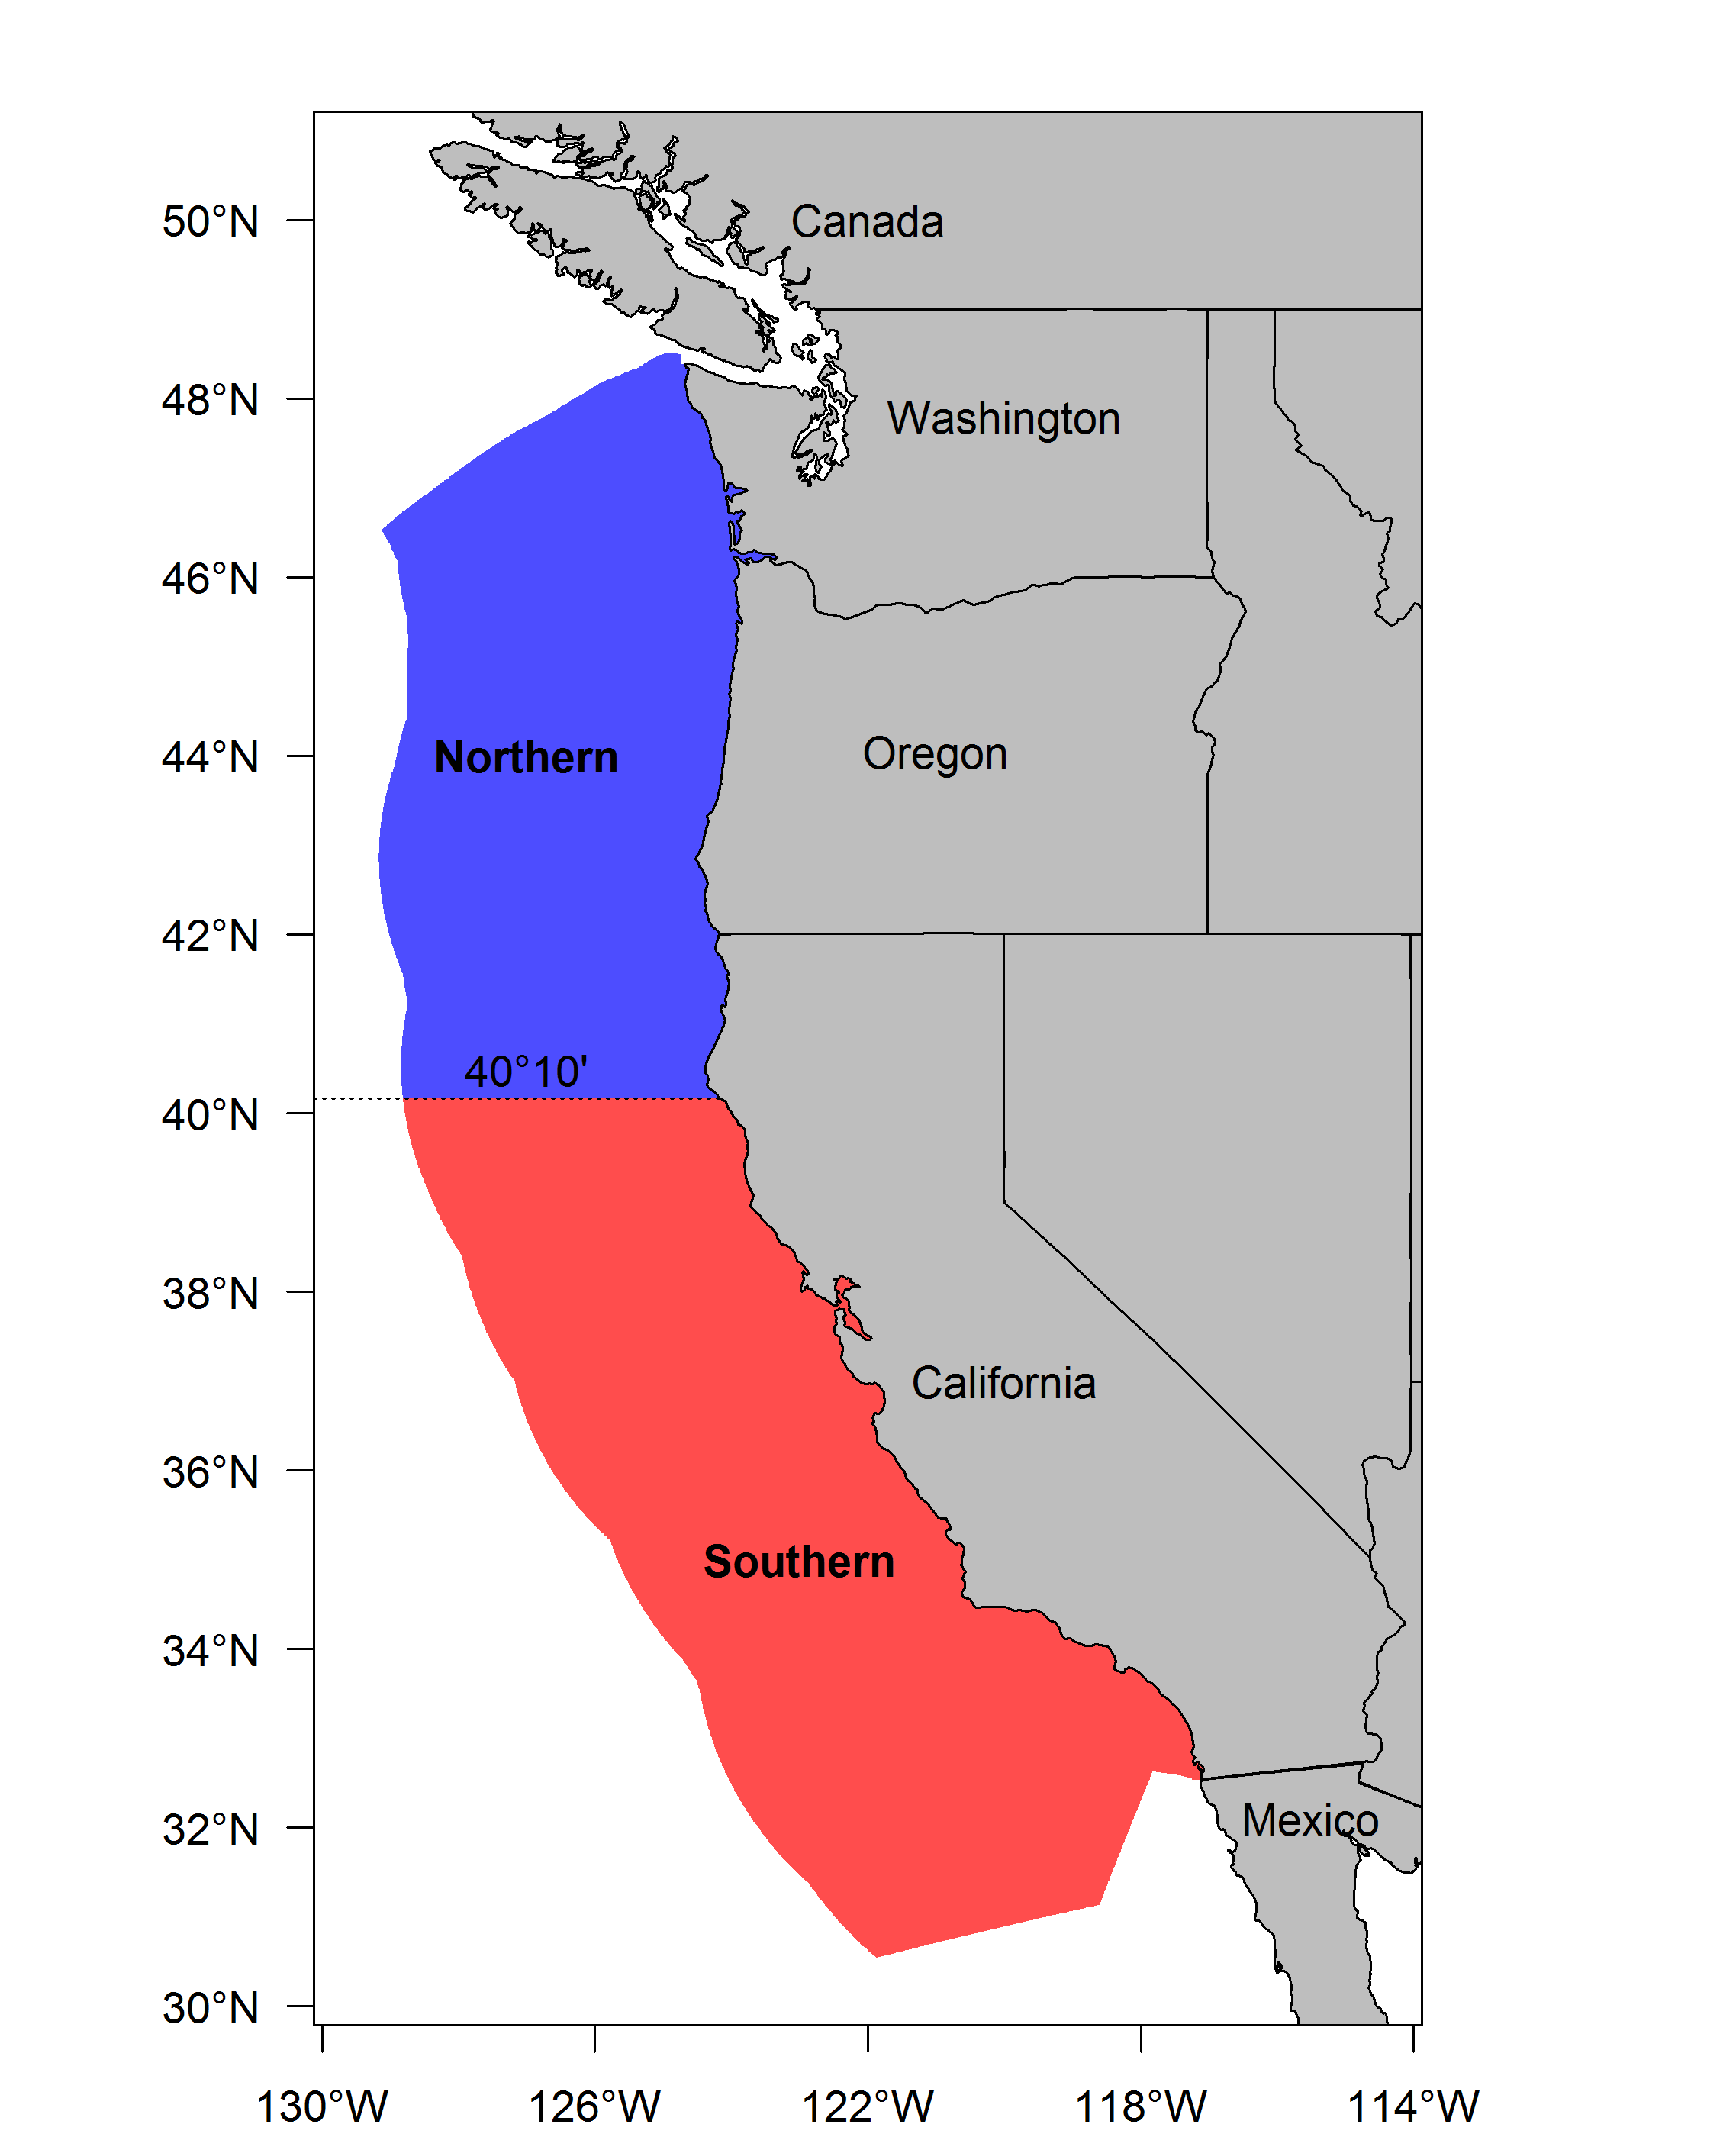
\includegraphics{Figures/assess_region_map_v2.png}
\caption{Map depicting the boundaries for the base-case model.
\label{fig:assess_region_map}}
\end{figure}

\begin{figure}[htbp]
\centering
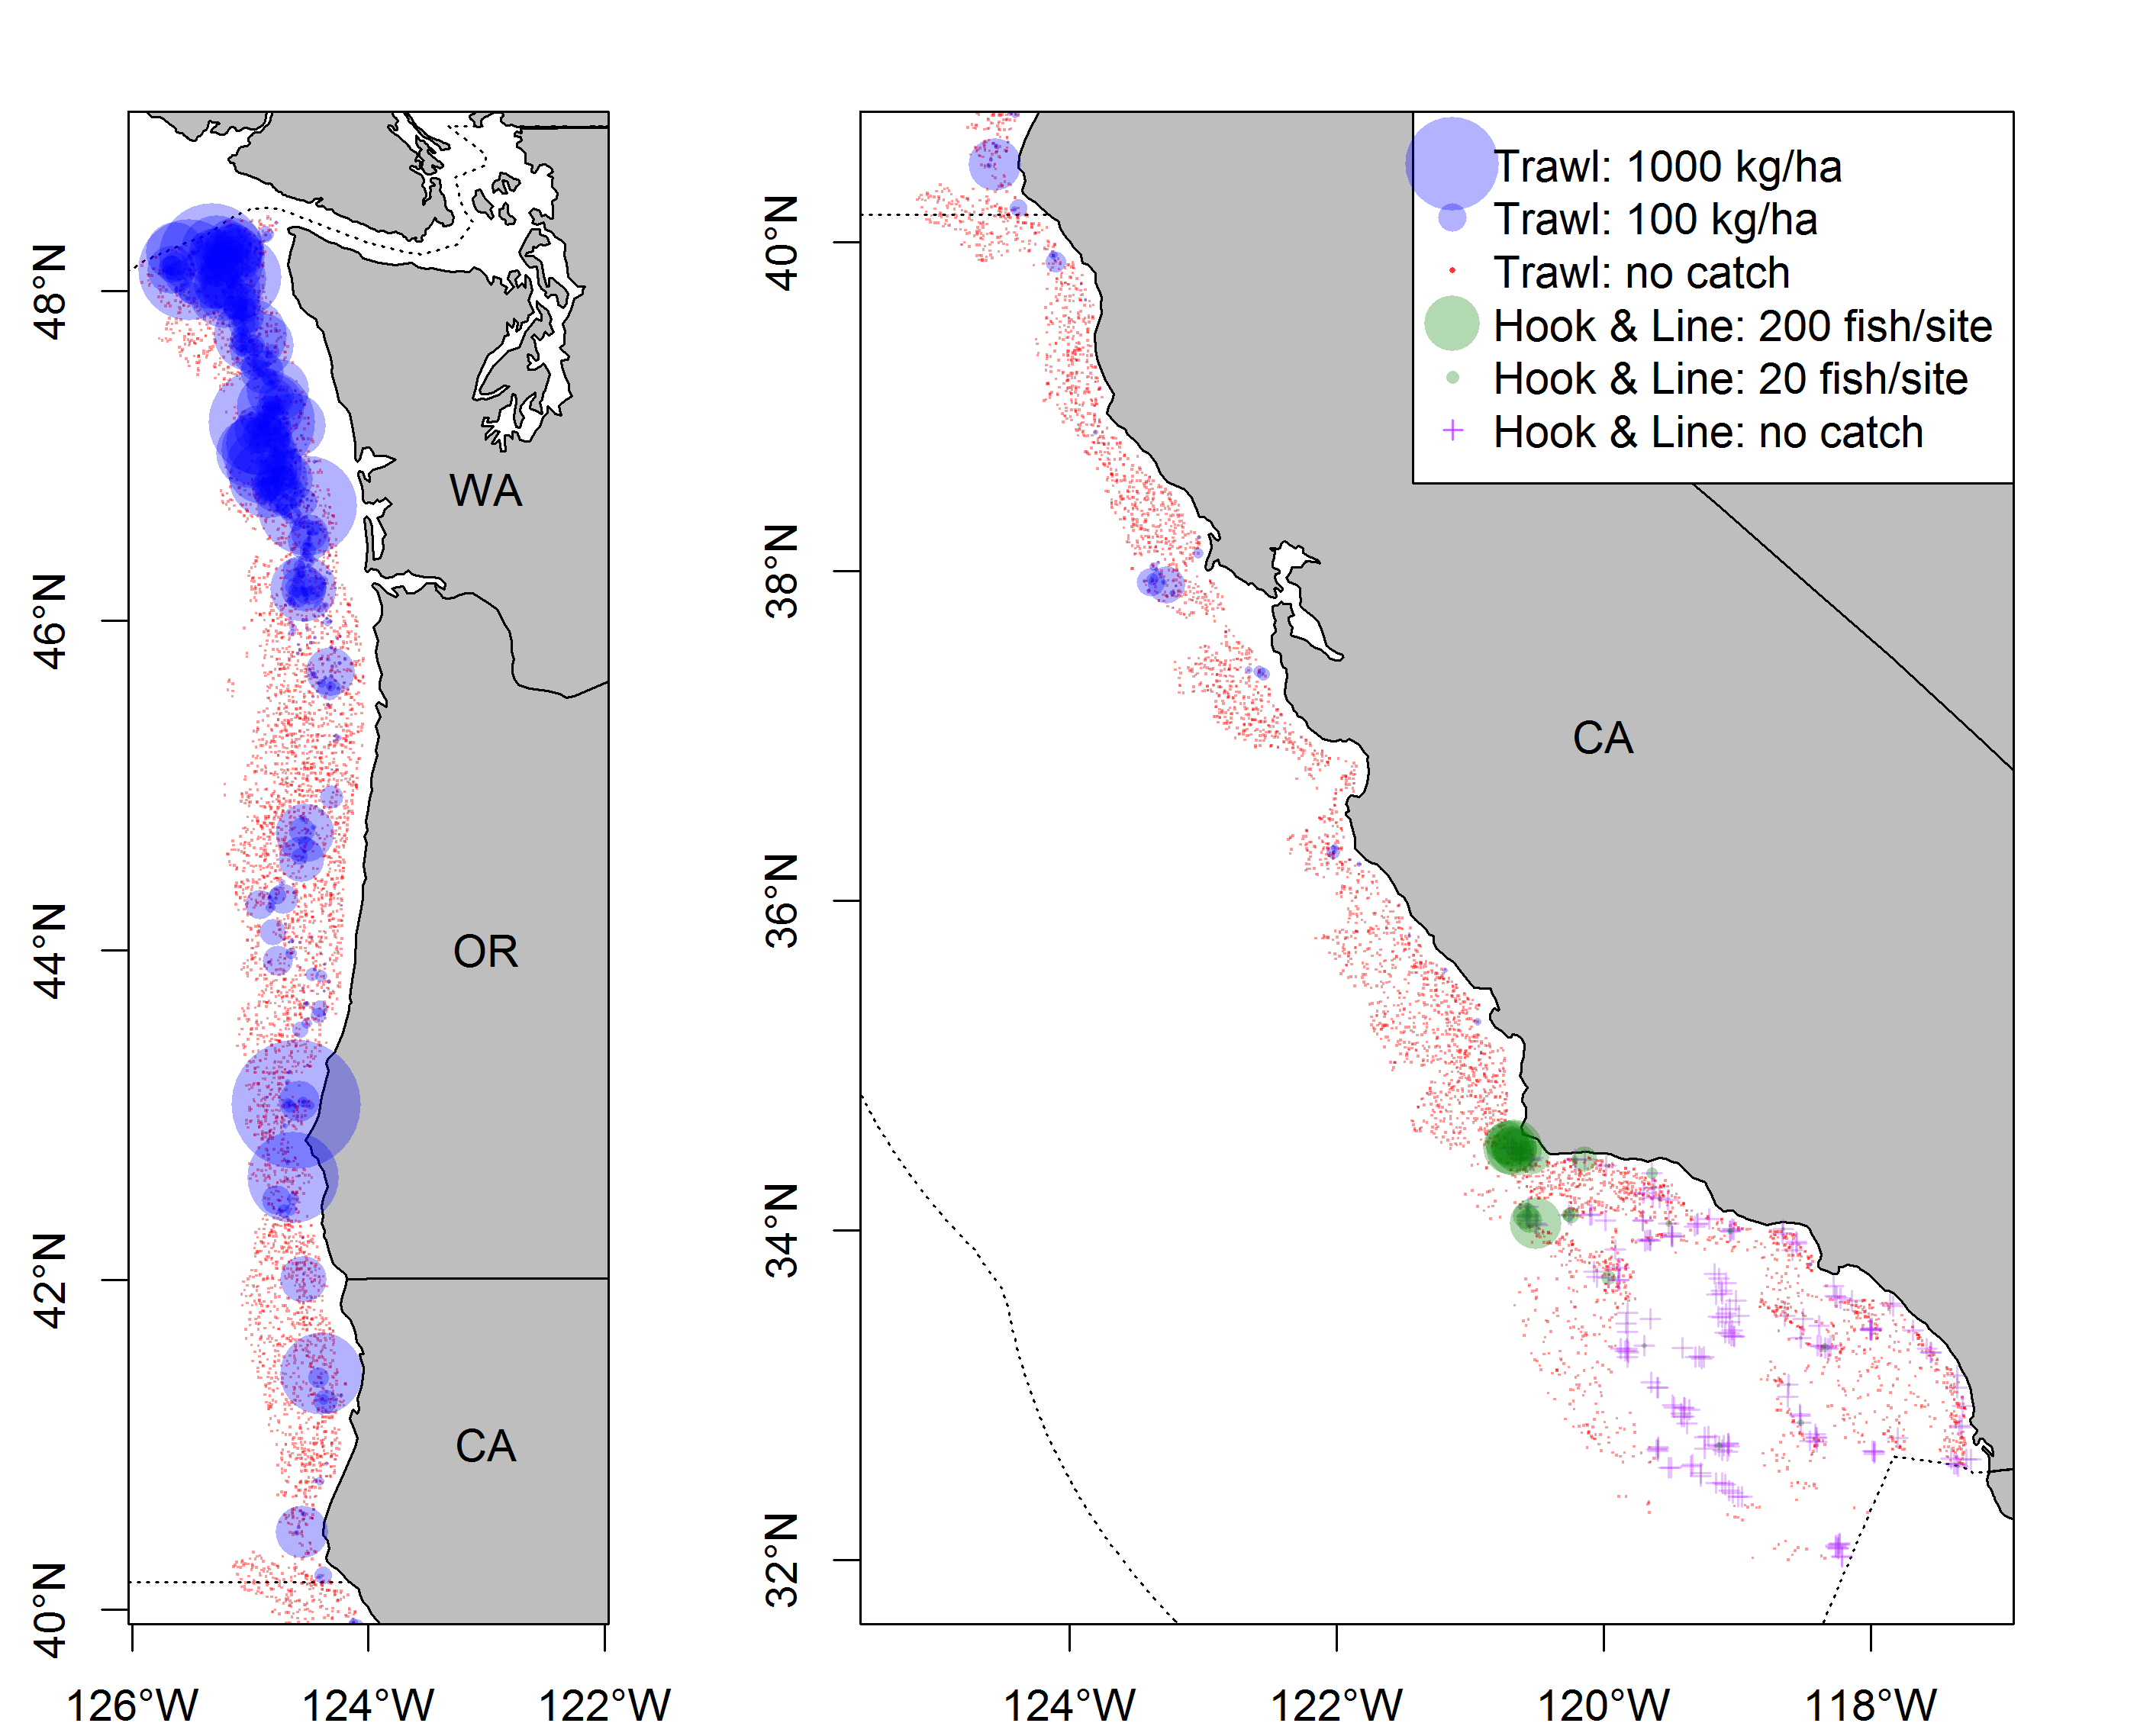
\includegraphics{Figures/survey_hauls_map.png}
\caption{Map showing observations of Yellowtail Rockfish in the
NWFSCcombo trawl survey and Hook \& Line survey.
\label{fig:assess_region_map}}
\end{figure}

\newpage

\subsection{Life history (maturity, fecundity, and growth) for both
models}\label{life-history-maturity-fecundity-and-growth-for-both-models}

\begin{figure}[htbp]
\centering
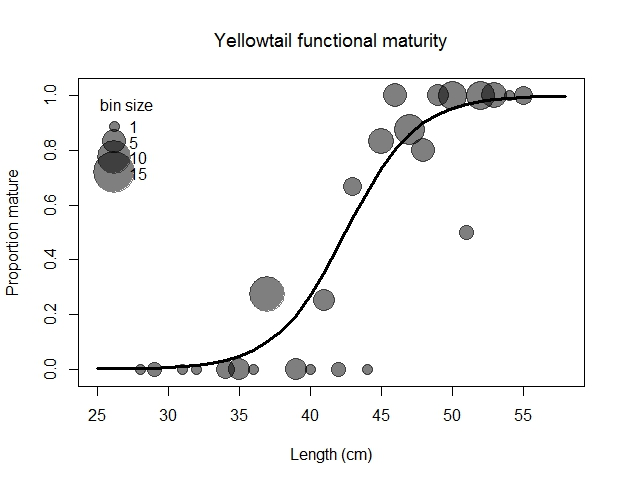
\includegraphics{Figures/YT_Propmat_update3_22.jpeg}
\caption{Estimated maturity relationship for Yellowtail Rockfish used in
both models. Gray points indicate average observed functional maturity
within each length bin with point size proportional to the number of
samples.\label{fig:maturity}}
\end{figure}

\begin{figure}[htbp]
\centering
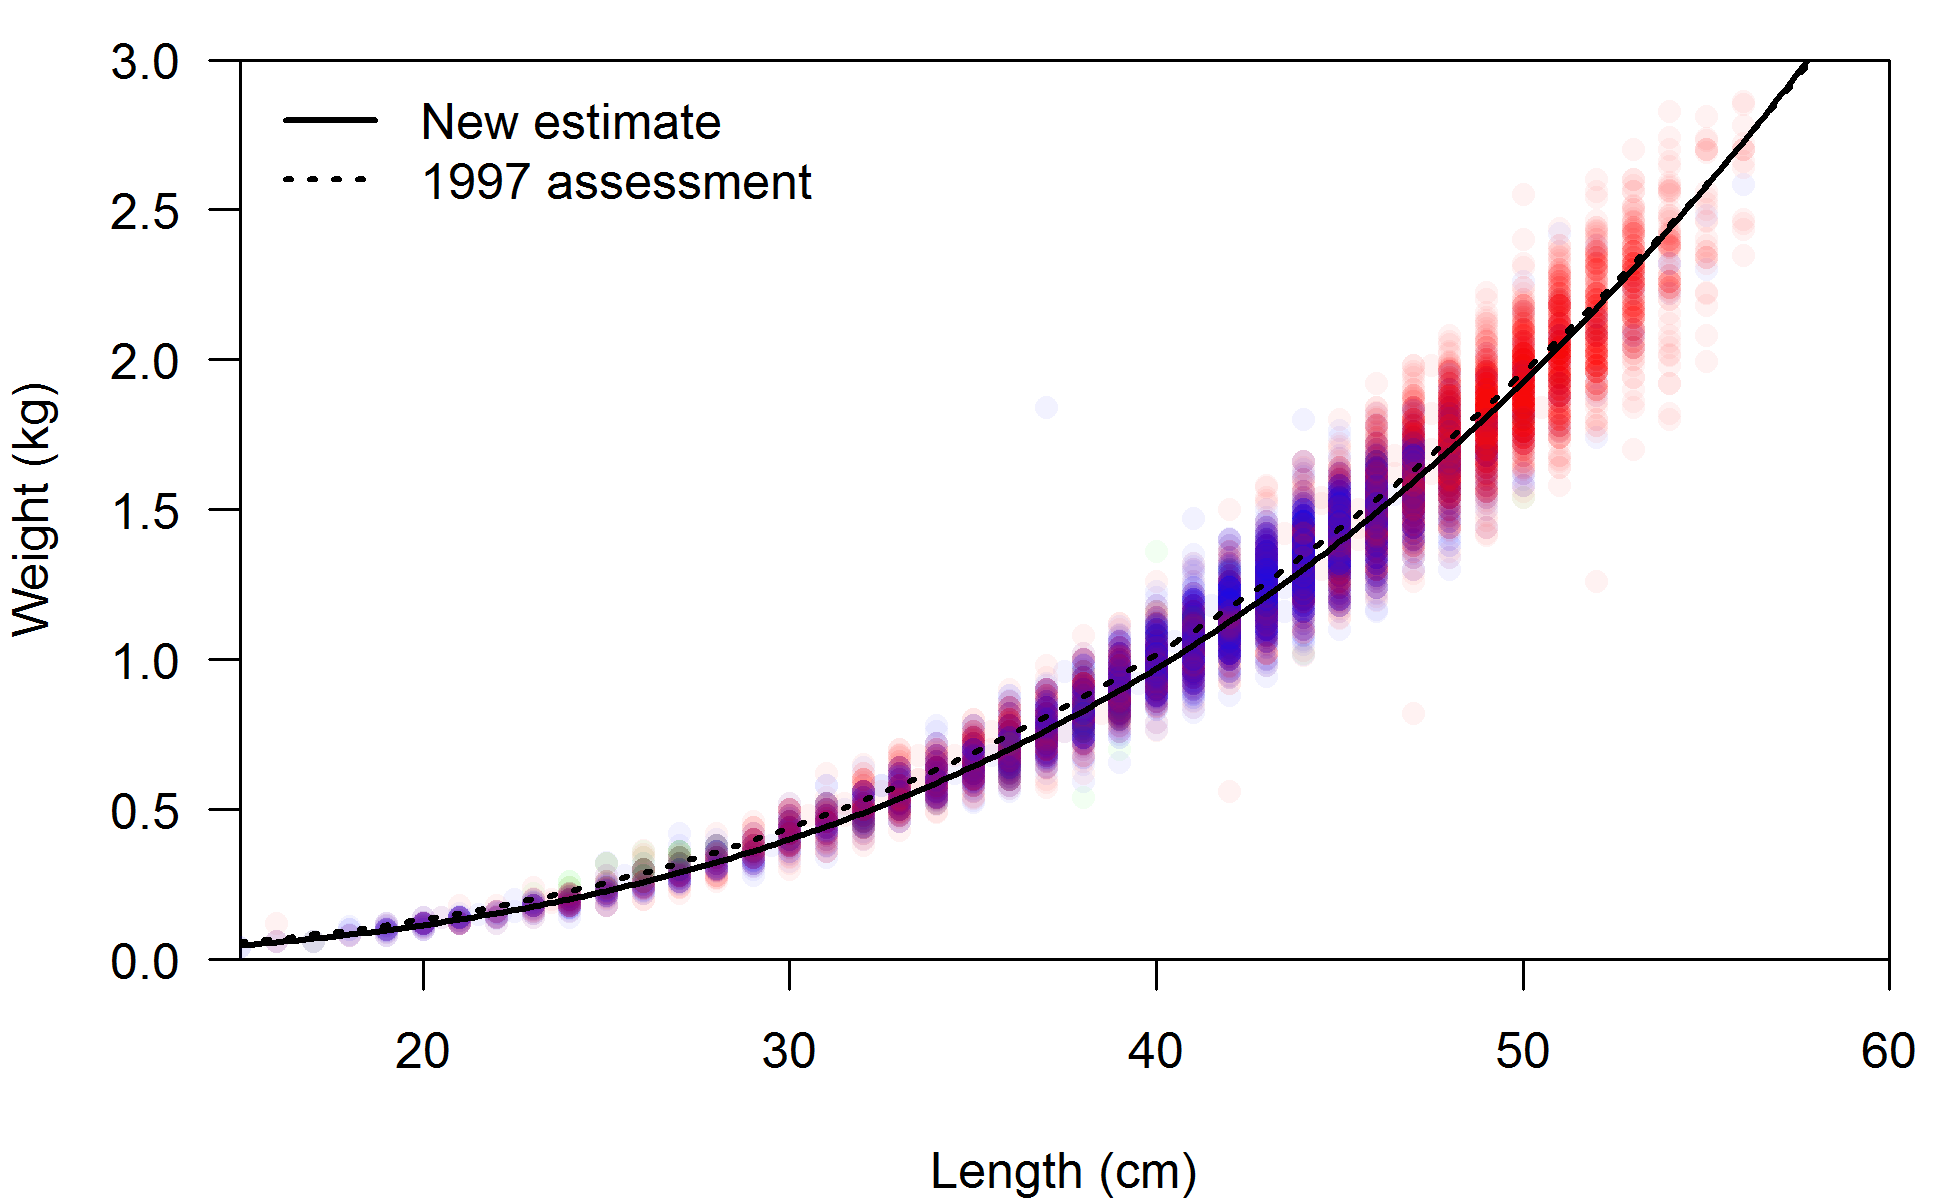
\includegraphics{Figures/weight-length_fit.png}
\caption{Estimated weight-length relationship for Yellowtail Rockfish
used in both models. Colored points show observed values (red for
females, blue for males, and green for unsexed). The black line
indicates the estimated relationship
\(W = 0.000011843L^{3.0672}\).\label{fig:weight-length}}
\end{figure}

\begin{figure}[htbp]
\centering
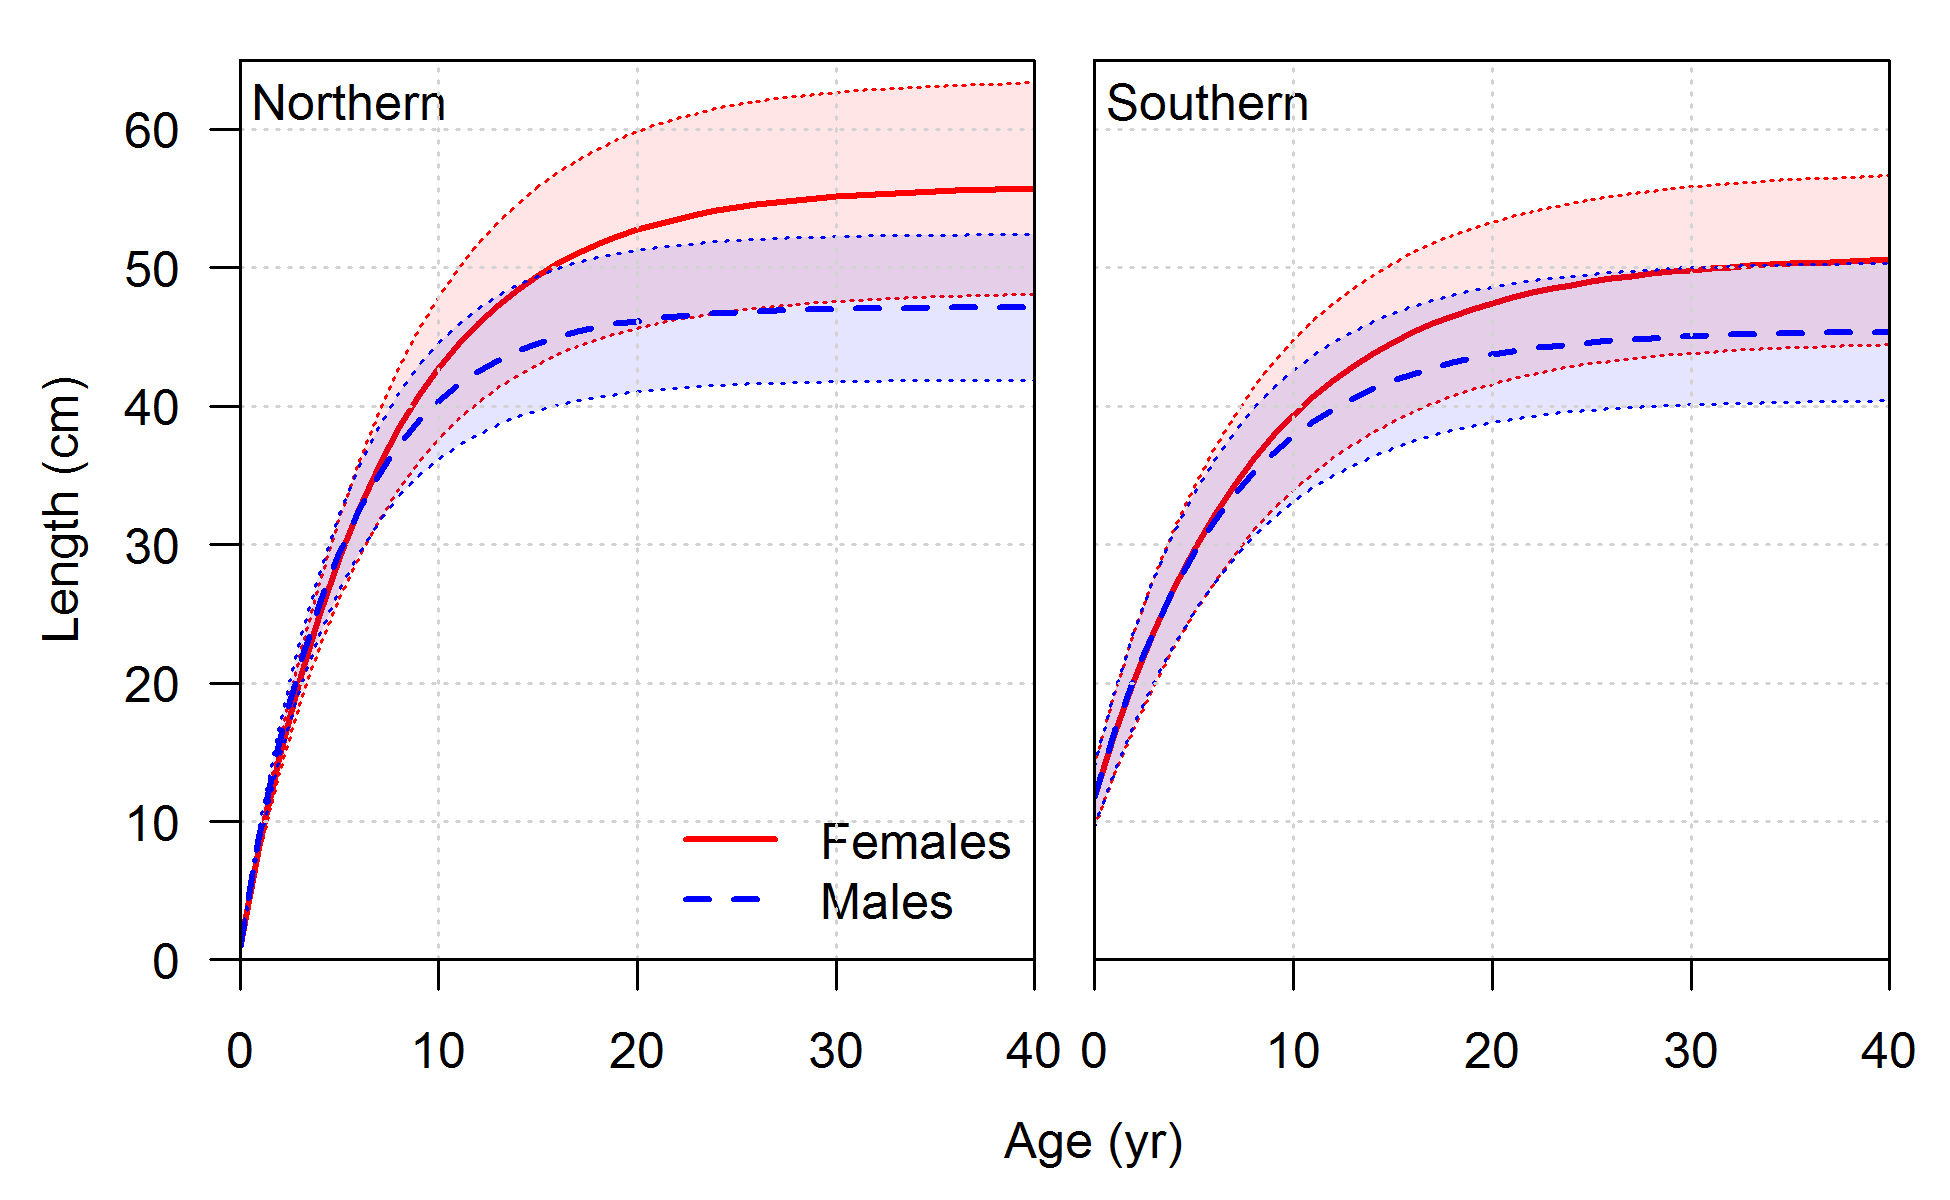
\includegraphics{r4ss/plots_compare/growth_comparison.png}
\caption{Estimated length-at-age for female and male Yellowtail Rockfish
in each model. Shaded areas indicate 95\% intervals for distribution of
lengths at each age. Values represent beginning-of-year growth.
\label{fig:growth}}
\end{figure}

\FloatBarrier 

\newpage

\subsection{Data and model fits for the Northern
model}\label{data-and-model-fits-for-the-northern-model}

\begin{figure}[htbp]
\centering
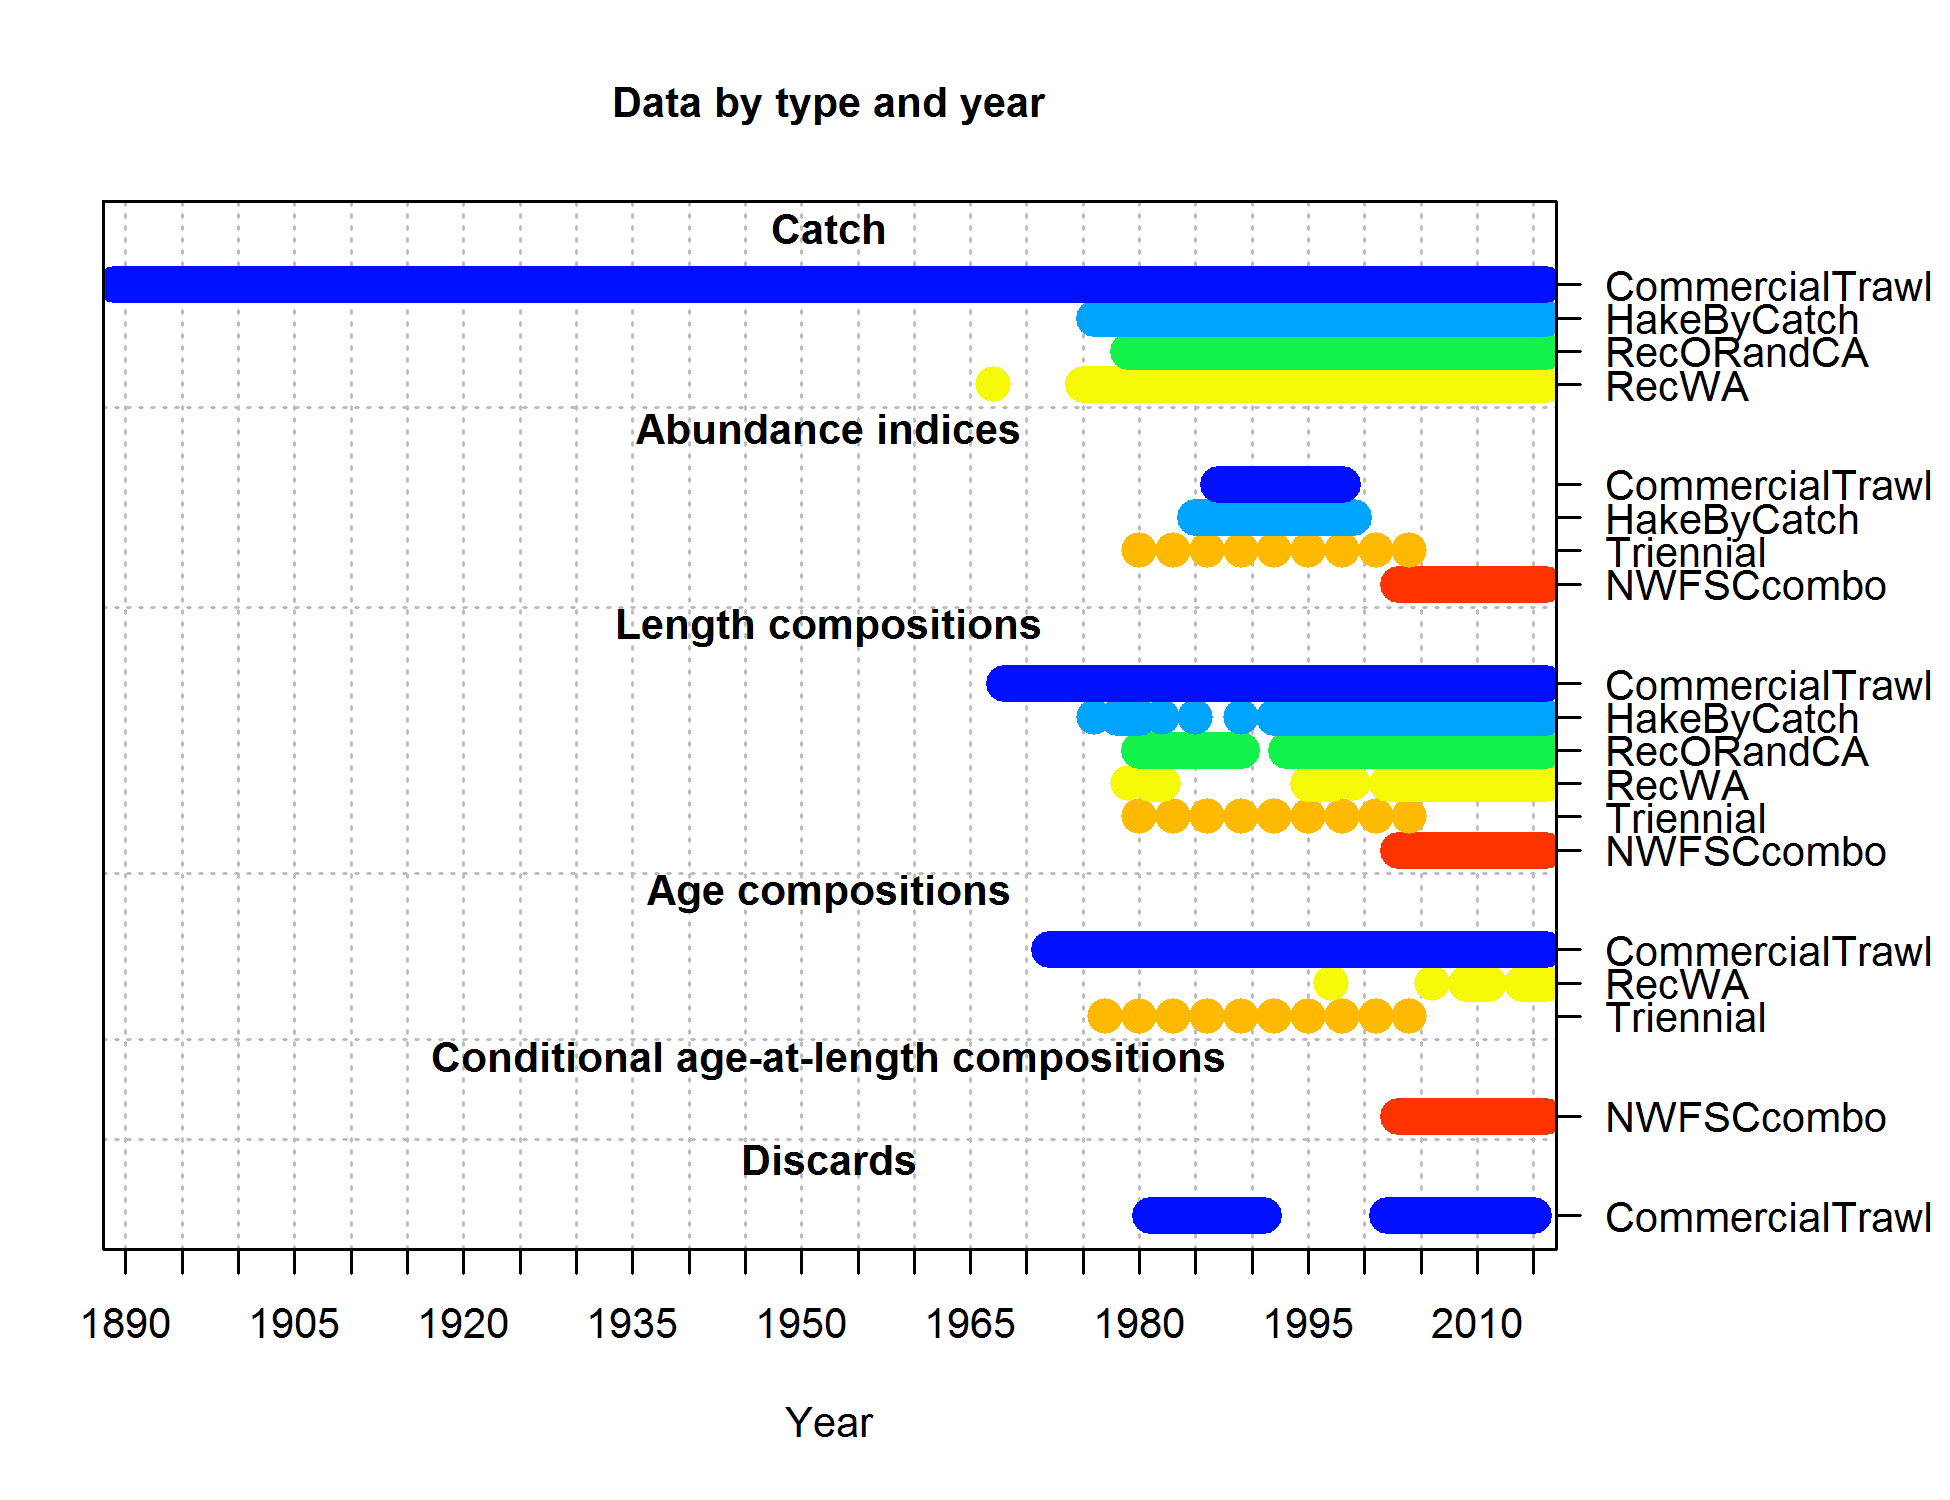
\includegraphics{r4ss/plots_mod1/data_plot.png}
\caption{Summary of data sources used in the Northern model.
\label{fig:data_plot}}
\end{figure}

\FloatBarrier

\begin{figure}[htbp]
\centering
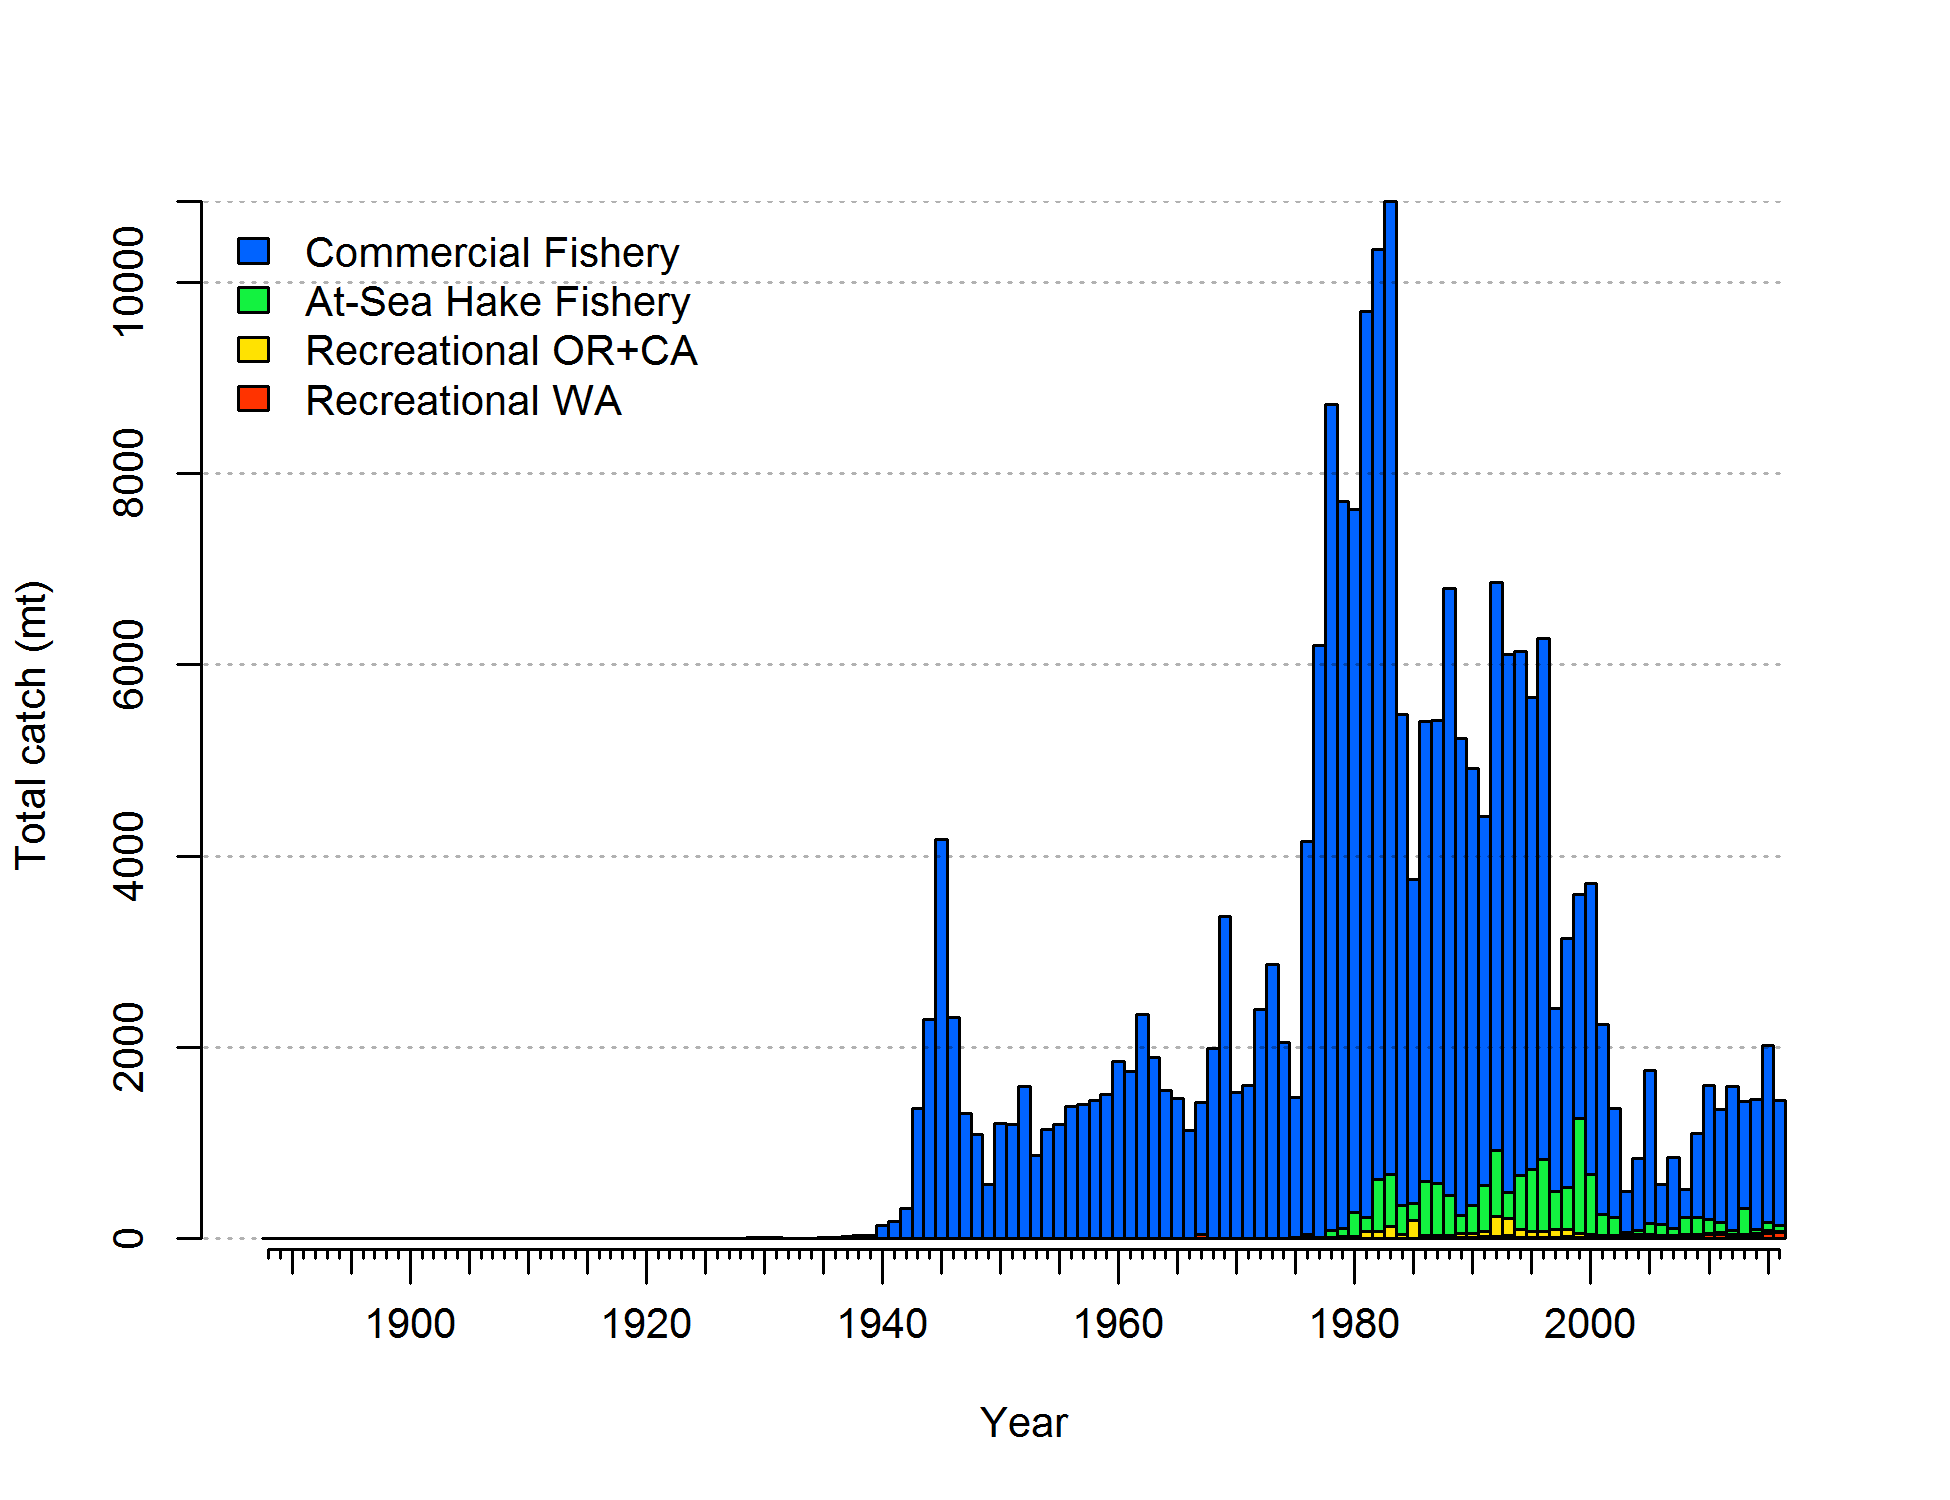
\includegraphics{r4ss/plots_mod1/catch5 total catch (including discards) stacked.png}
\caption{Estimated catch history of Yellowtail Rockfish in the Northern
model. Recreational catches in Washington are model estimates of total
weigth converted from input catch in numbers using model estimates of
growth and selectivity. Catches for the Commercial Fishery include
estimated discards.\label{fig:r4ss_total_catch_N}}
\end{figure}

\begin{figure}[htbp]
\centering
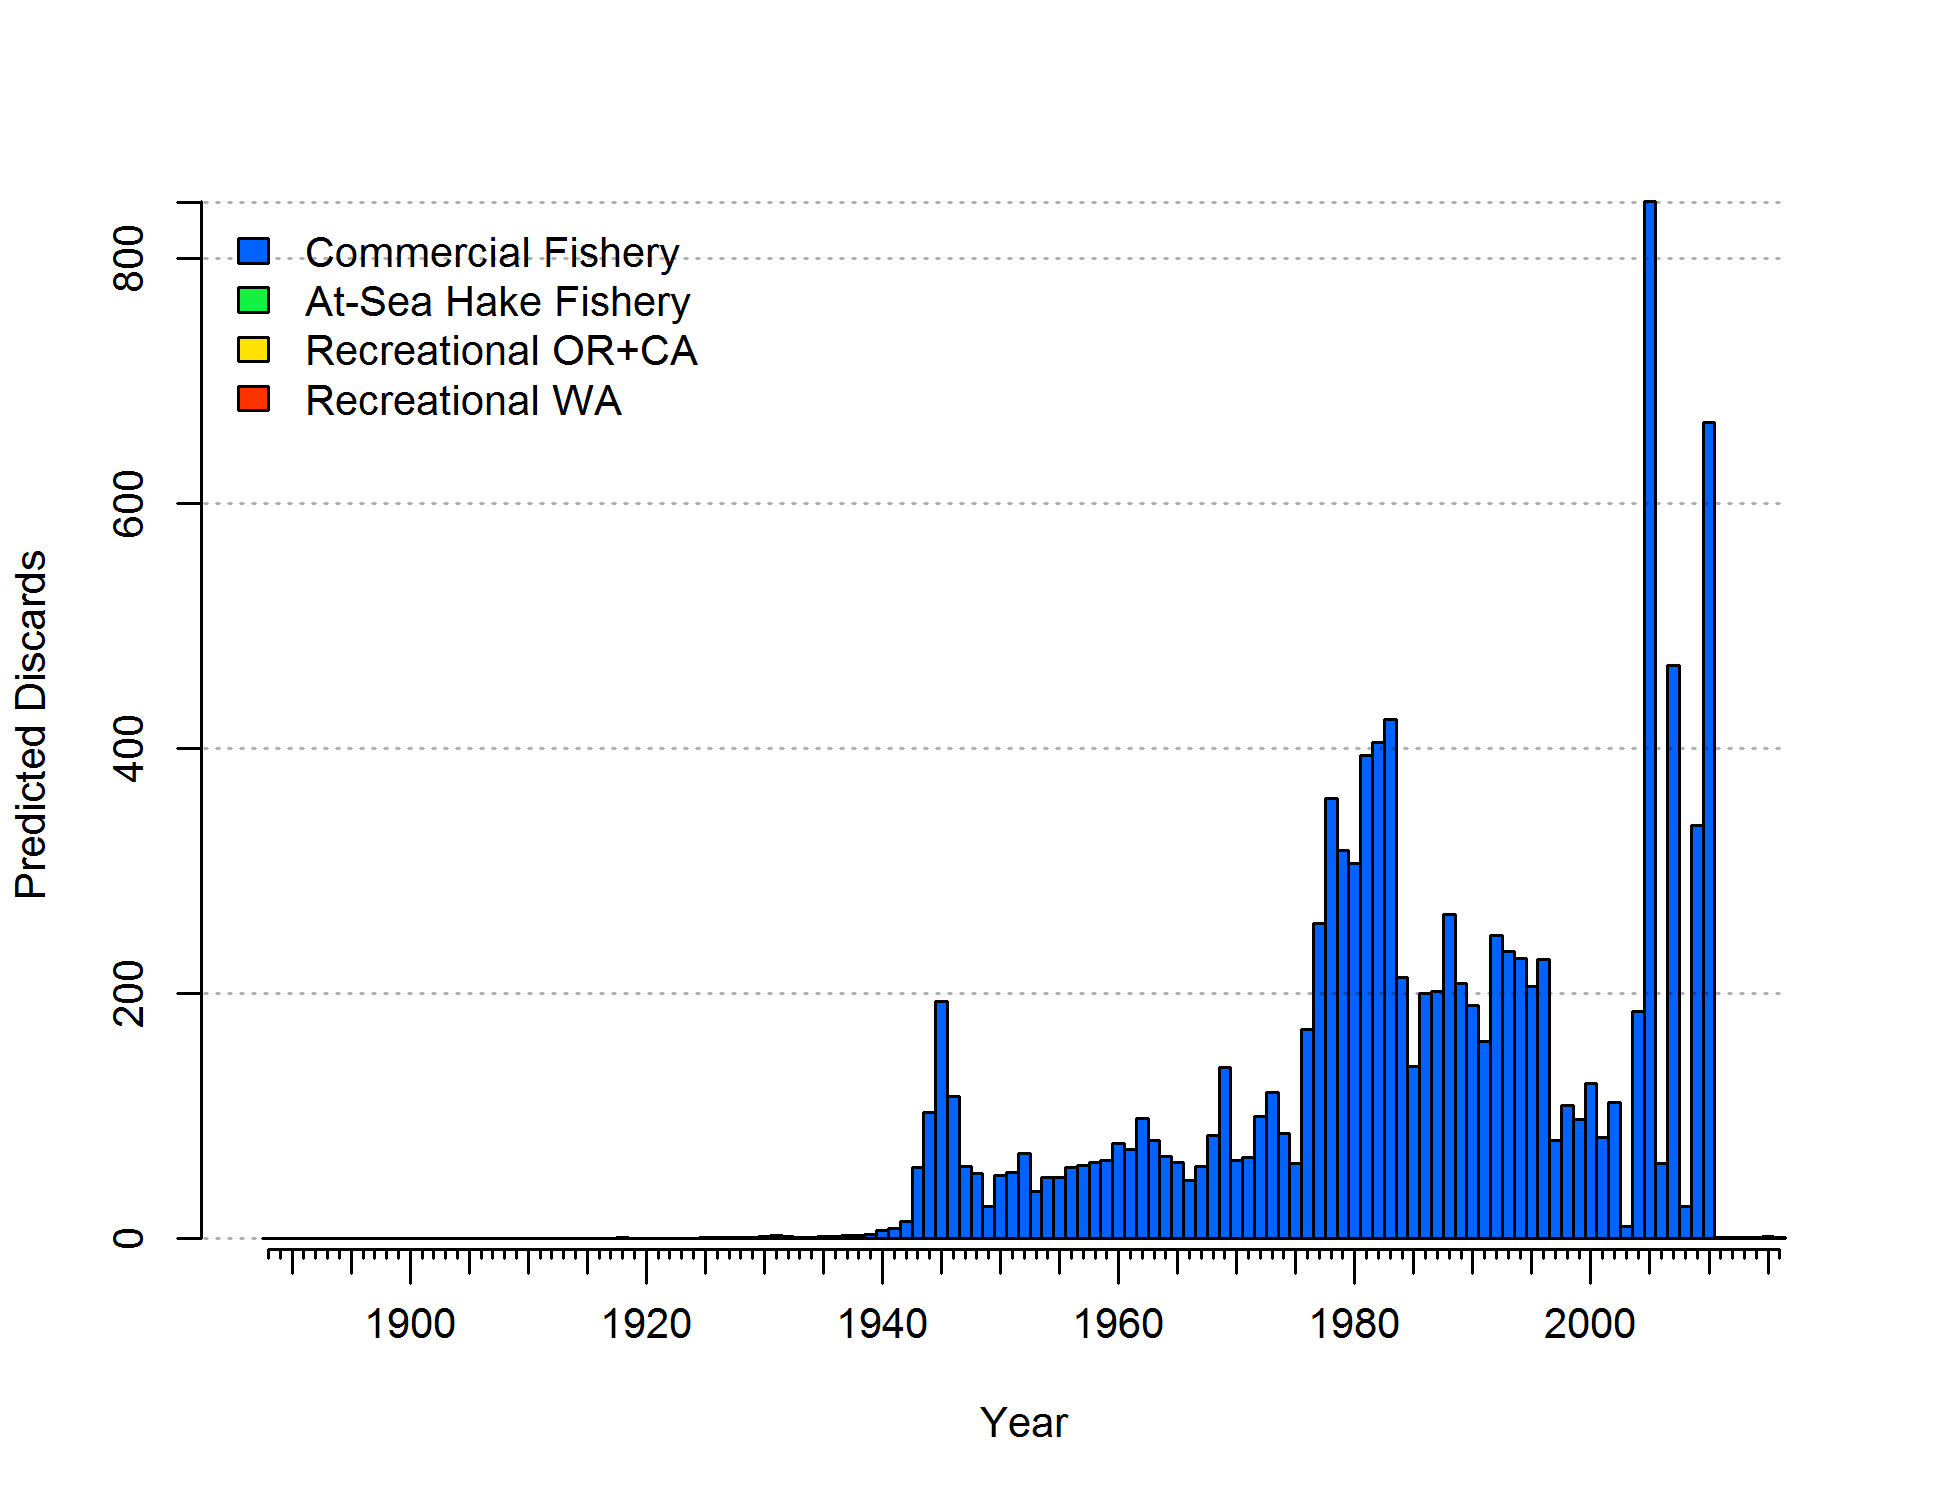
\includegraphics{r4ss/plots_mod1/catch7 discards stacked plot (depends on multiple fleets).png}
\caption{Estimated discards in the Commercial Fishery in the Northern
model. Estimates are influenced by the data for landings, discard
ratios, and discard length combines and depend on the estimated
parameters controlling selectivity and
retention.\label{fig:r4ss_discard_N}}
\end{figure}

\FloatBarrier

\newpage 

\subsubsection{Selectivity, retention, and discards for Northern
model}\label{selectivity-retention-and-discards-for-northern-model}

\begin{figure}[htbp]
\centering
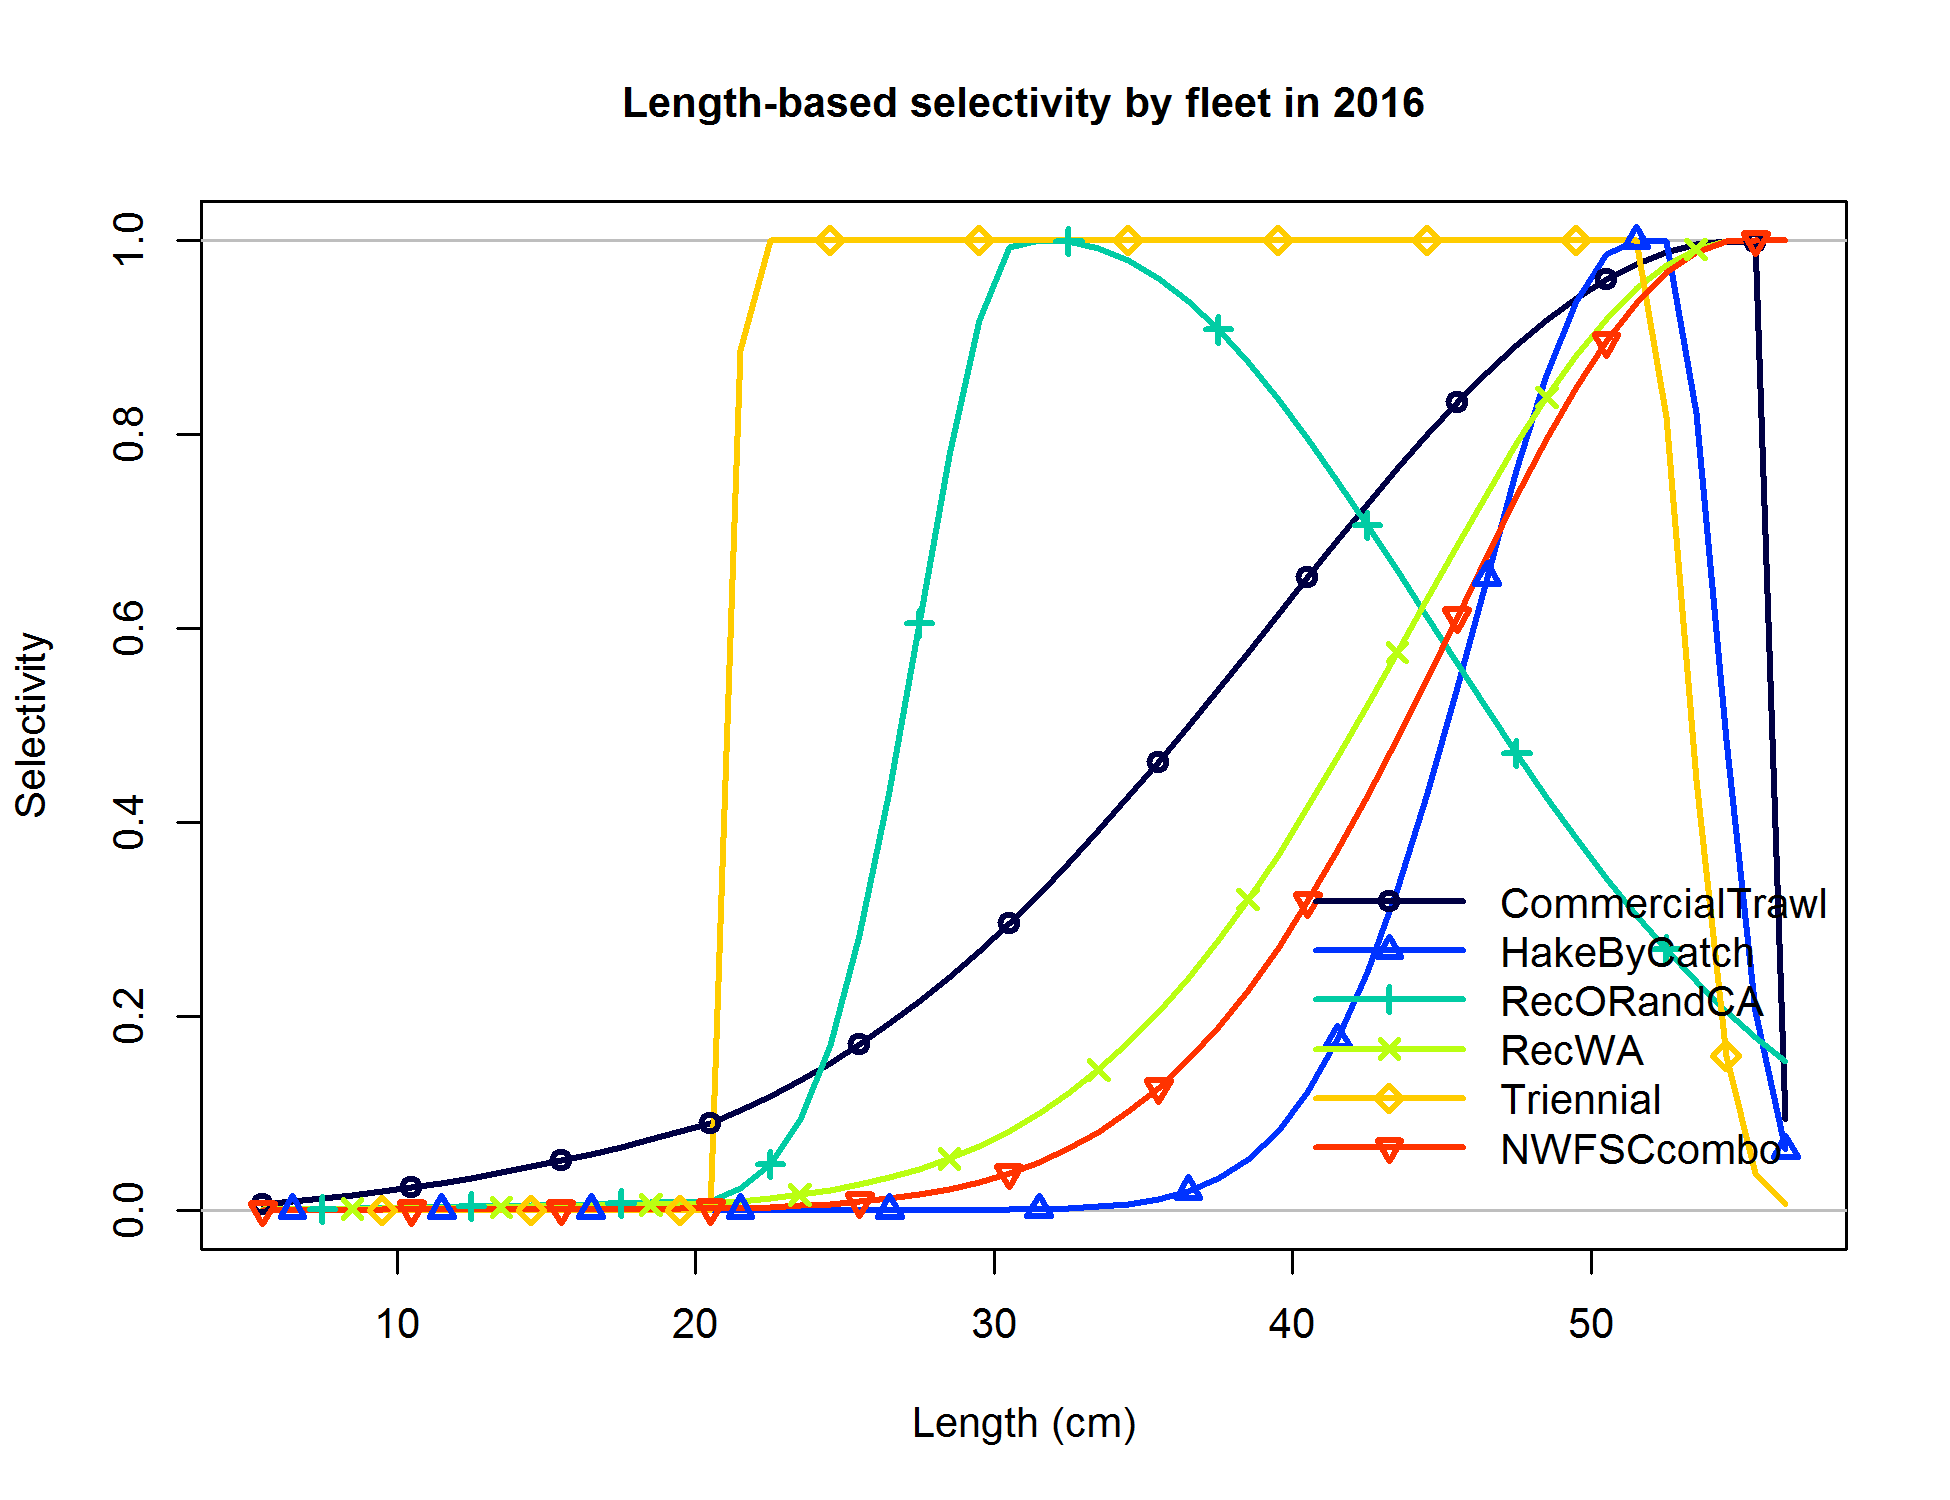
\includegraphics{r4ss/plots_mod1/sel01_multiple_fleets_length1.png}
\caption{Estimated selectivity by length by each fishery and survey in
the Northern model. \label{fig:selex}}
\end{figure}

\begin{figure}[htbp]
\centering
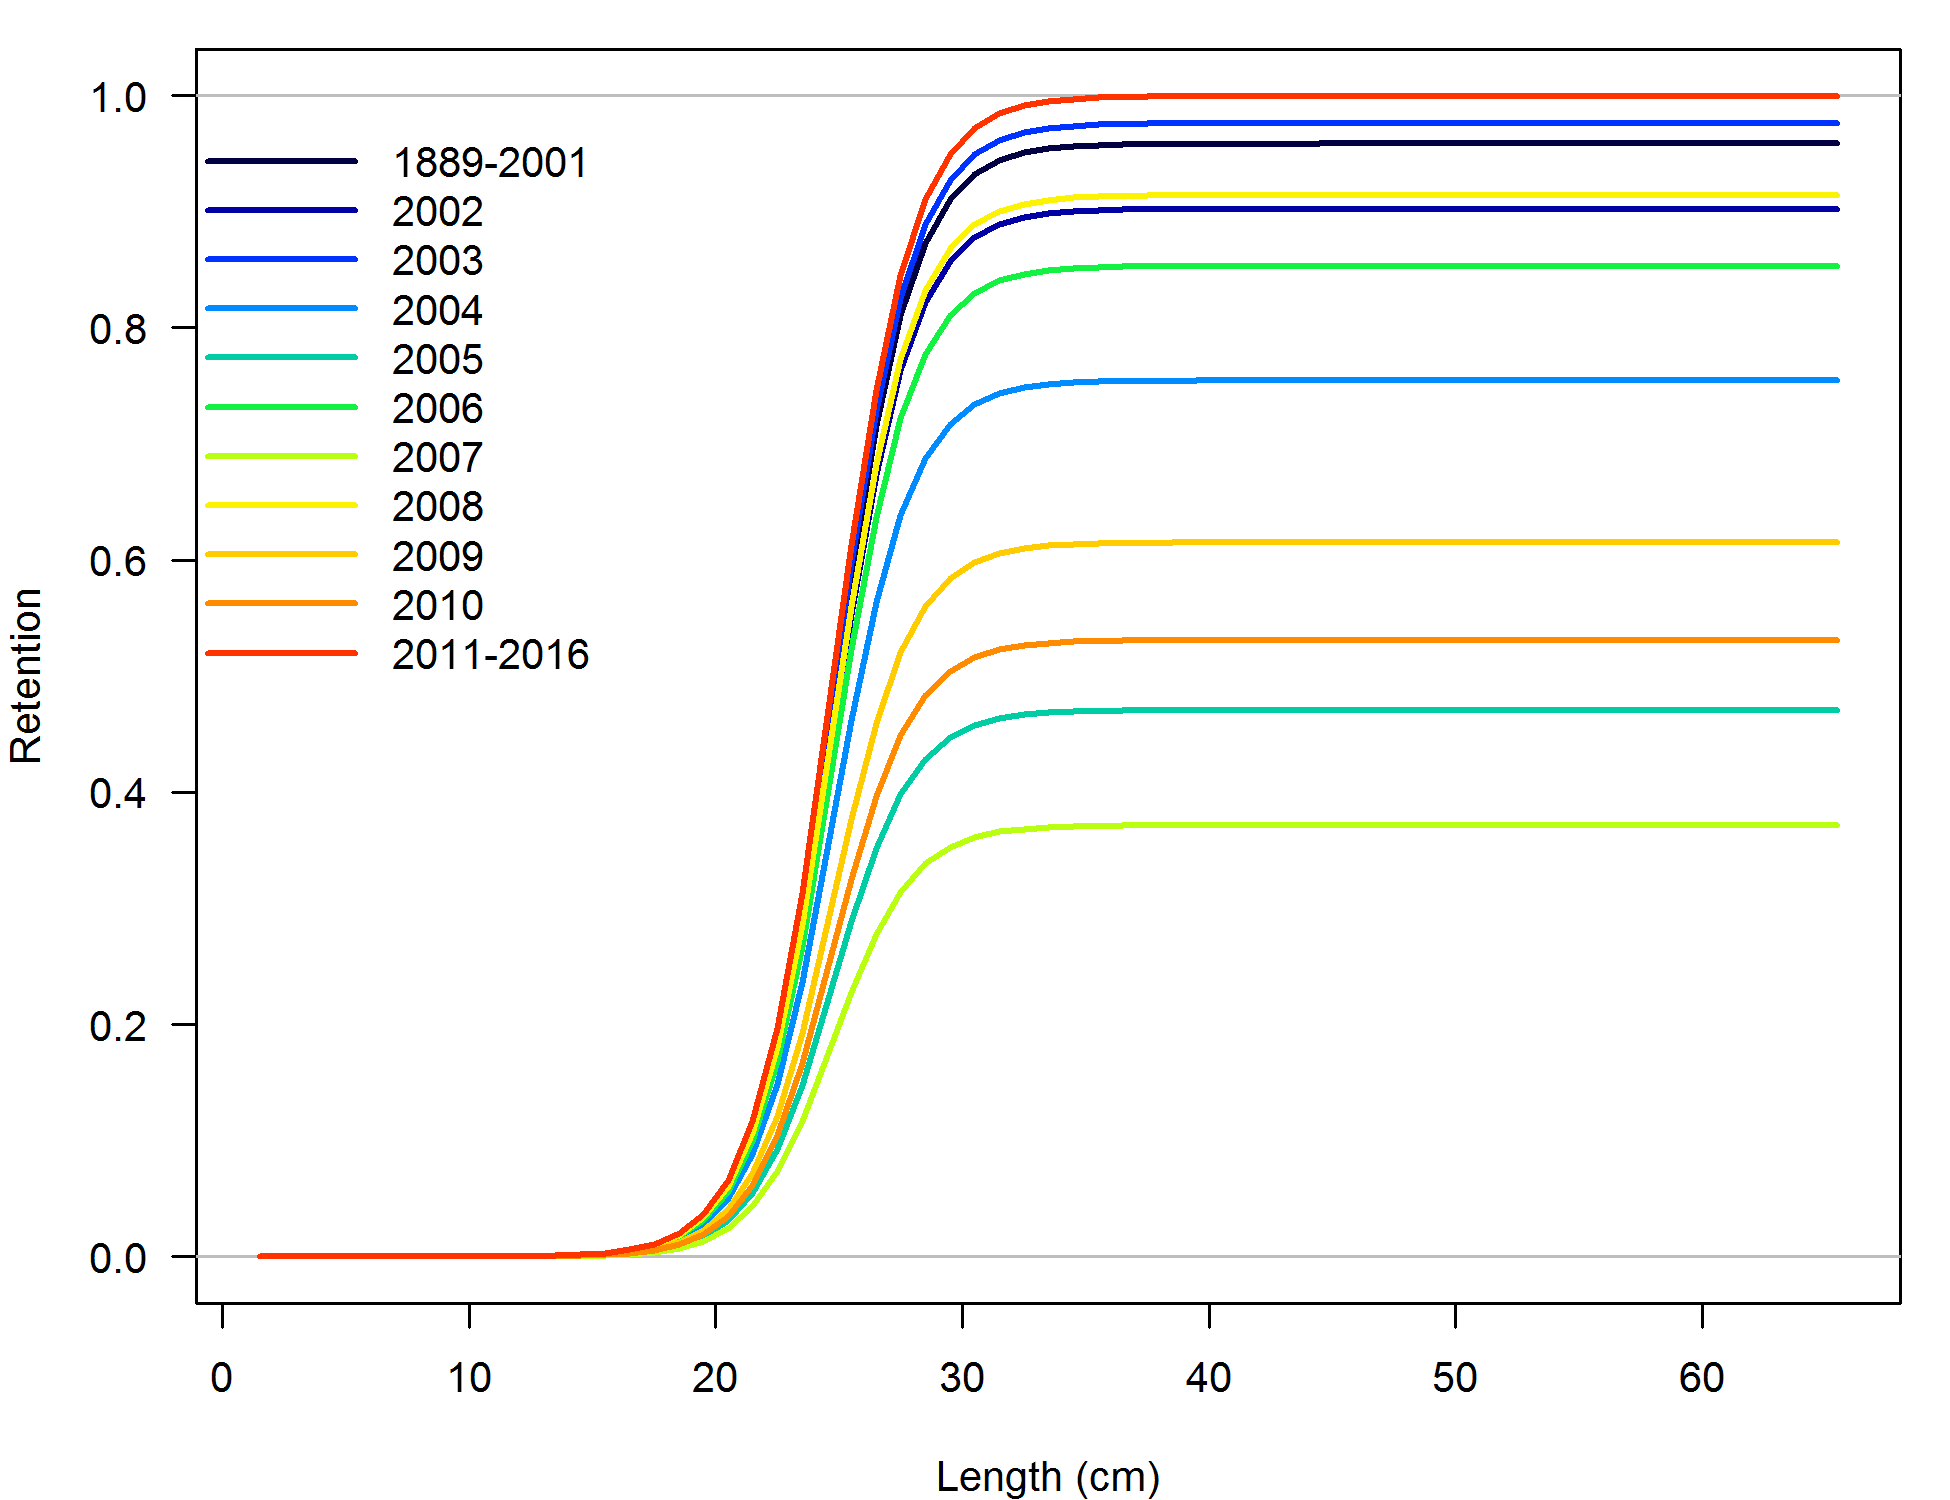
\includegraphics{r4ss/plots_mod1/time-varying_retention.png}
\caption{Estimated retention by length by the Commercial Fishery in the
Northern model. \label{fig:retention}}
\end{figure}

\FloatBarrier

\newpage

\begin{figure}[htbp]
\centering
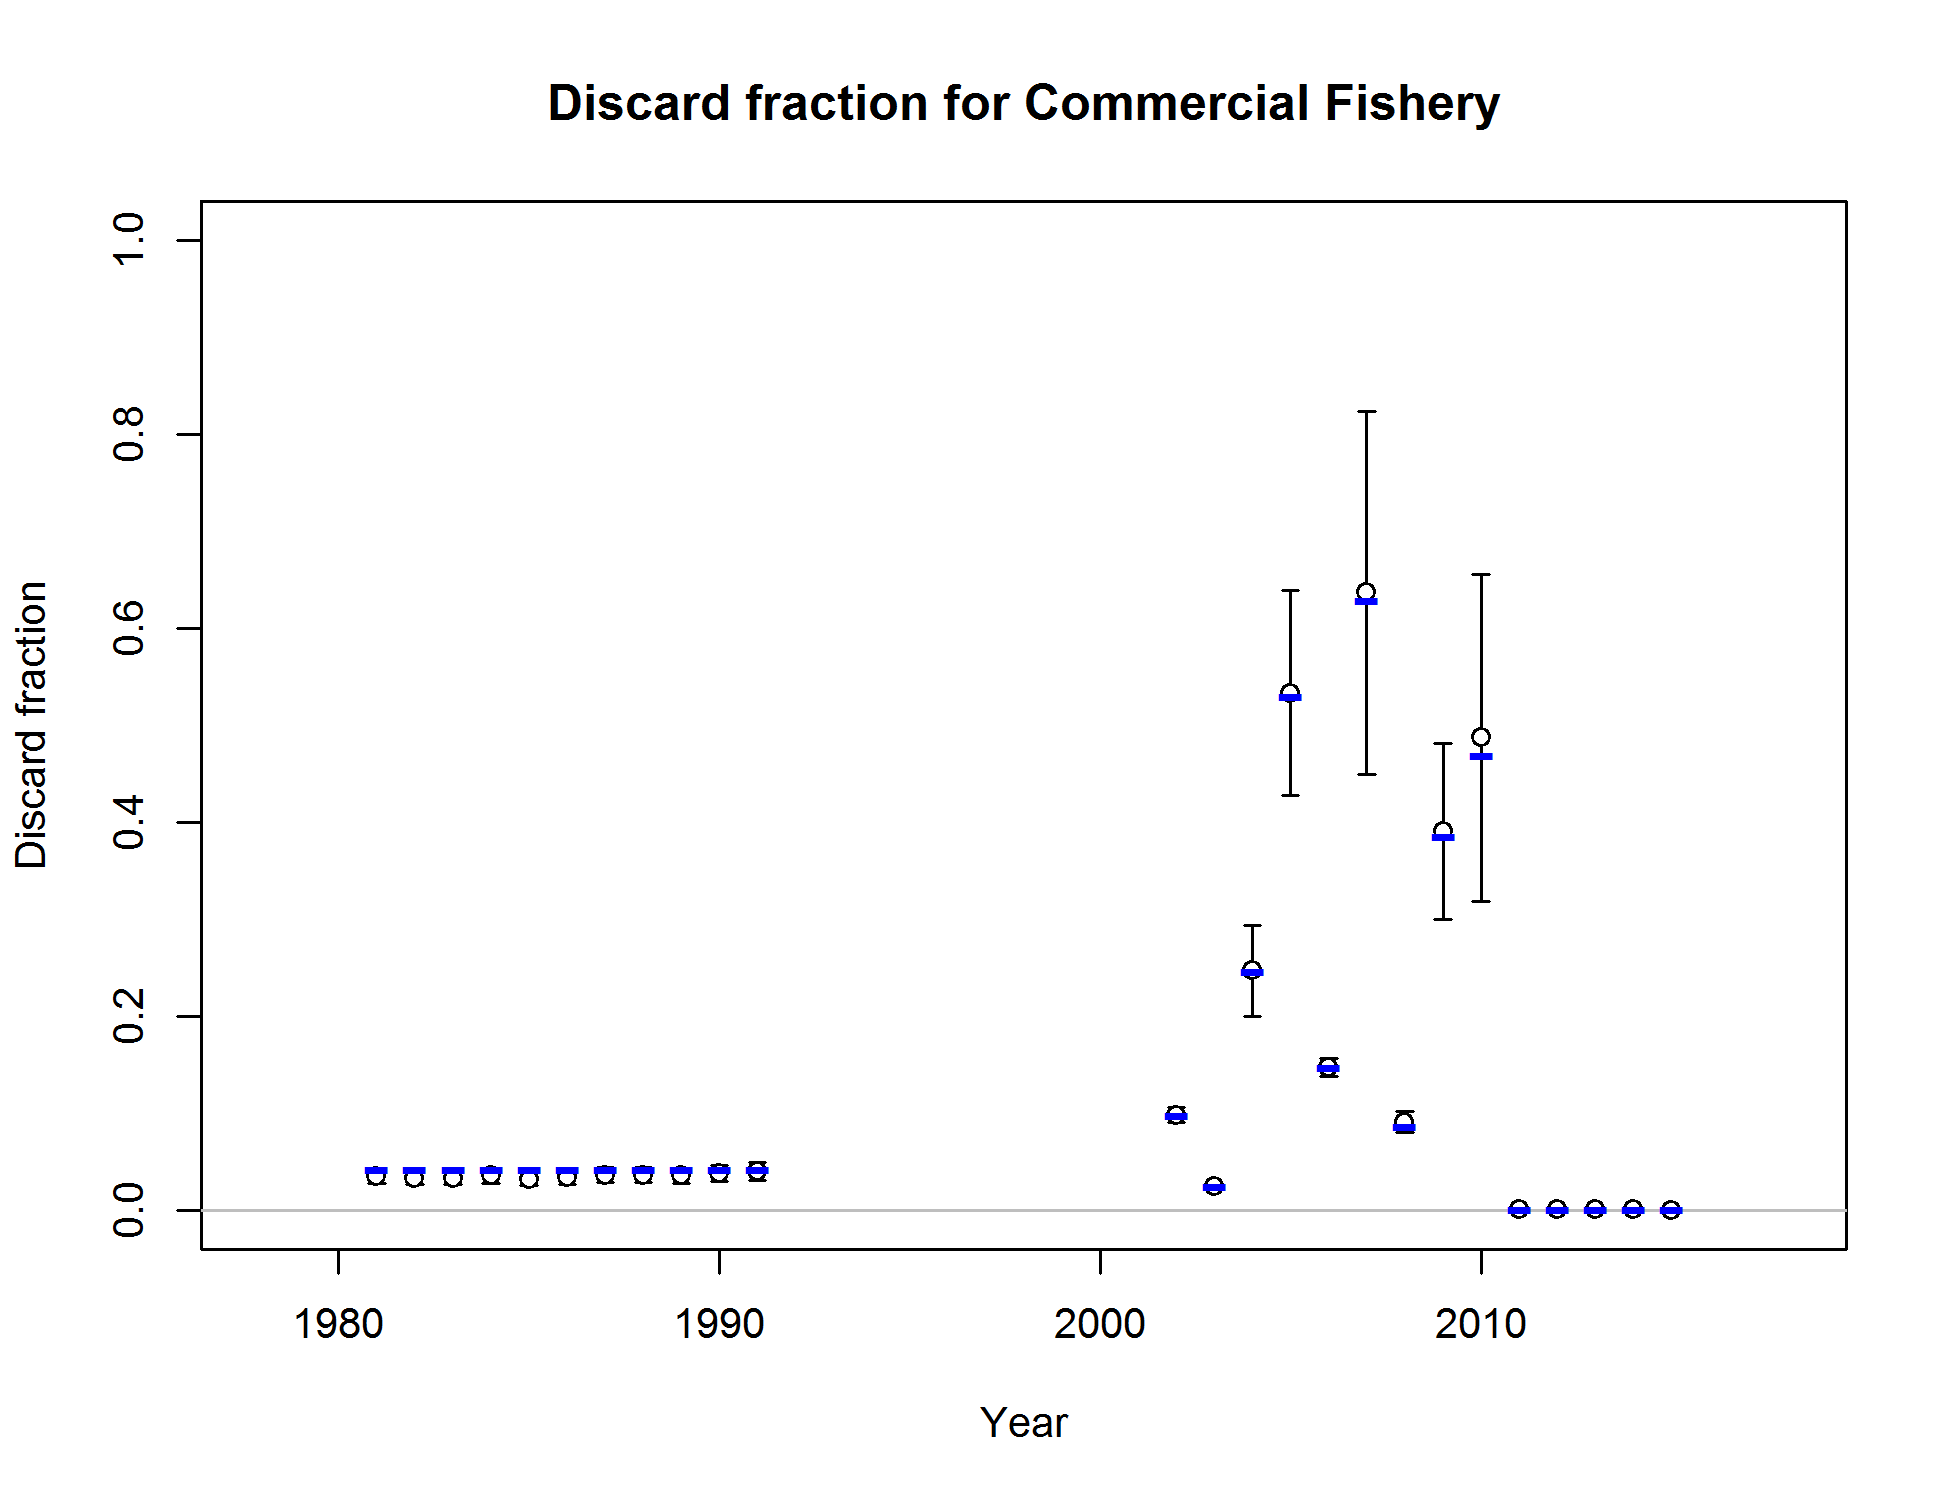
\includegraphics{r4ss/plots_mod1/discard_dataCommercial Fishery.png}
\caption{Fit to discard fractions for the commercial fishery in the
Northern model.\label{fig:r4ss_discard_fits}}
\end{figure}

\FloatBarrier

\newpage

\subsubsection{At-Sea Hake Bycatch
Index}\label{at-sea-hake-bycatch-index}

\begin{figure}[htbp]
\centering
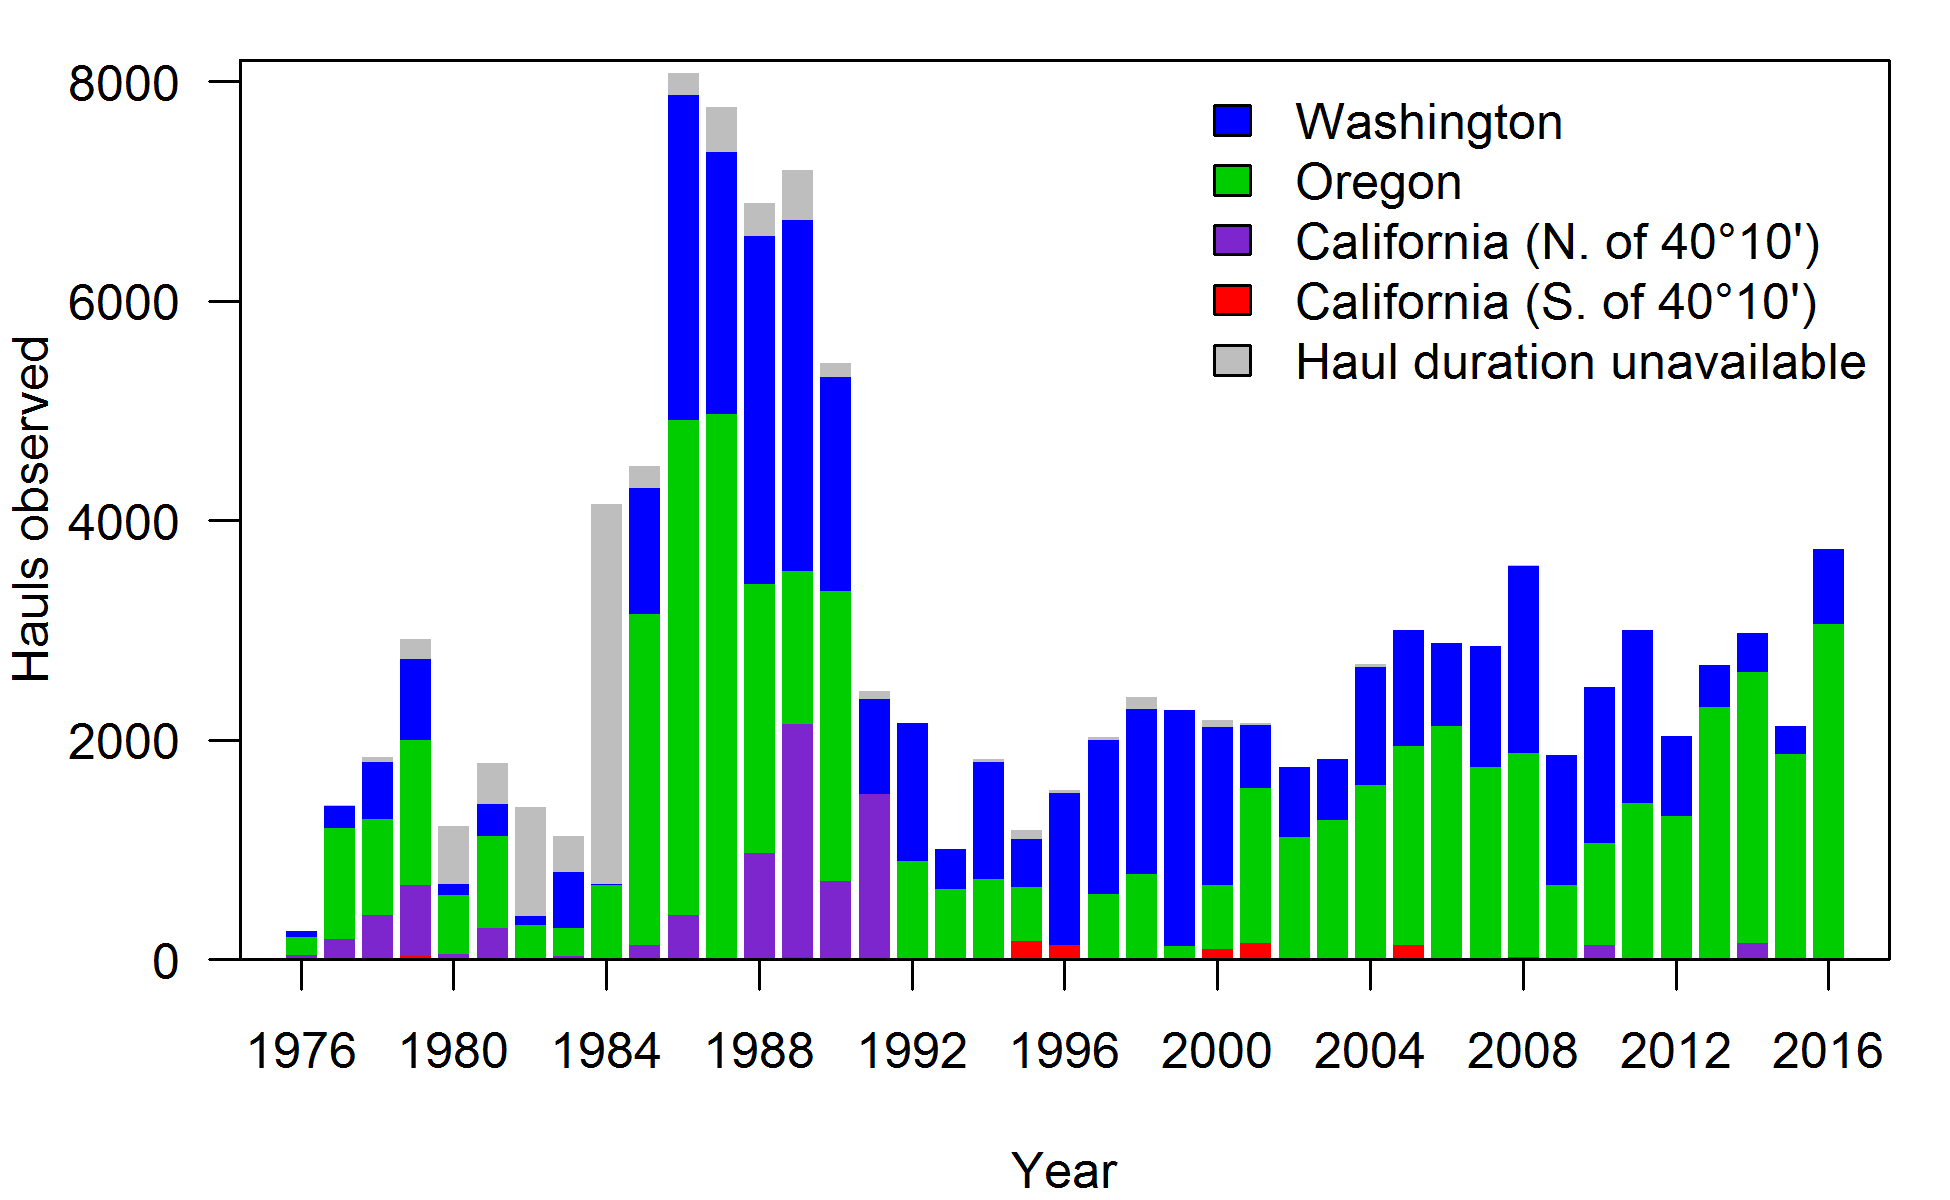
\includegraphics{Figures/ASHOP_hauls_observed_by_state.png}
\caption{Number of observed hauls from the at-sea hake fishery
classified by location relative to Washington, Oregon, and California
(north and south of 40-10). Grey bars indicate observed tows with no
haul duration available which were excluded from the CPUE
analysis.\label{fig:ASHOP_X1}}
\end{figure}

\begin{figure}[htbp]
\centering
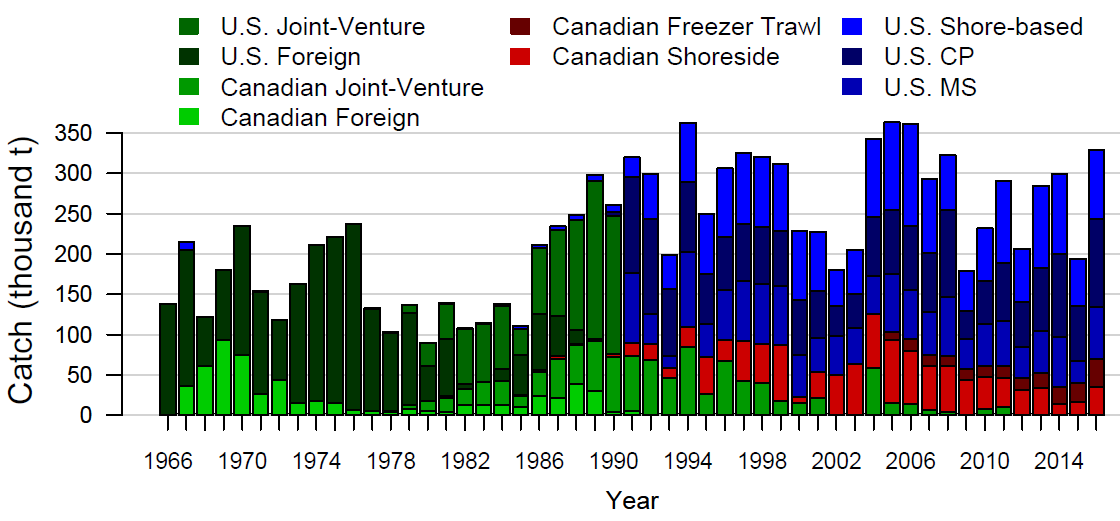
\includegraphics{Figures/Hake_fishery_catch_history.png}
\caption{Catch history for Pacific Hake by sector. Data used in the CPUE
analysis are from the ``U.S. Joint-Venture'' and ``U.S. Foreign
sectors'' through 1990 and from the Catcher-Processor (``U.S. CP'') and
Mothership (``U.S. MS'') sectors from 1990 onward.\label{fig:ASHOP_X2}}
\end{figure}

\begin{figure}[htbp]
\centering
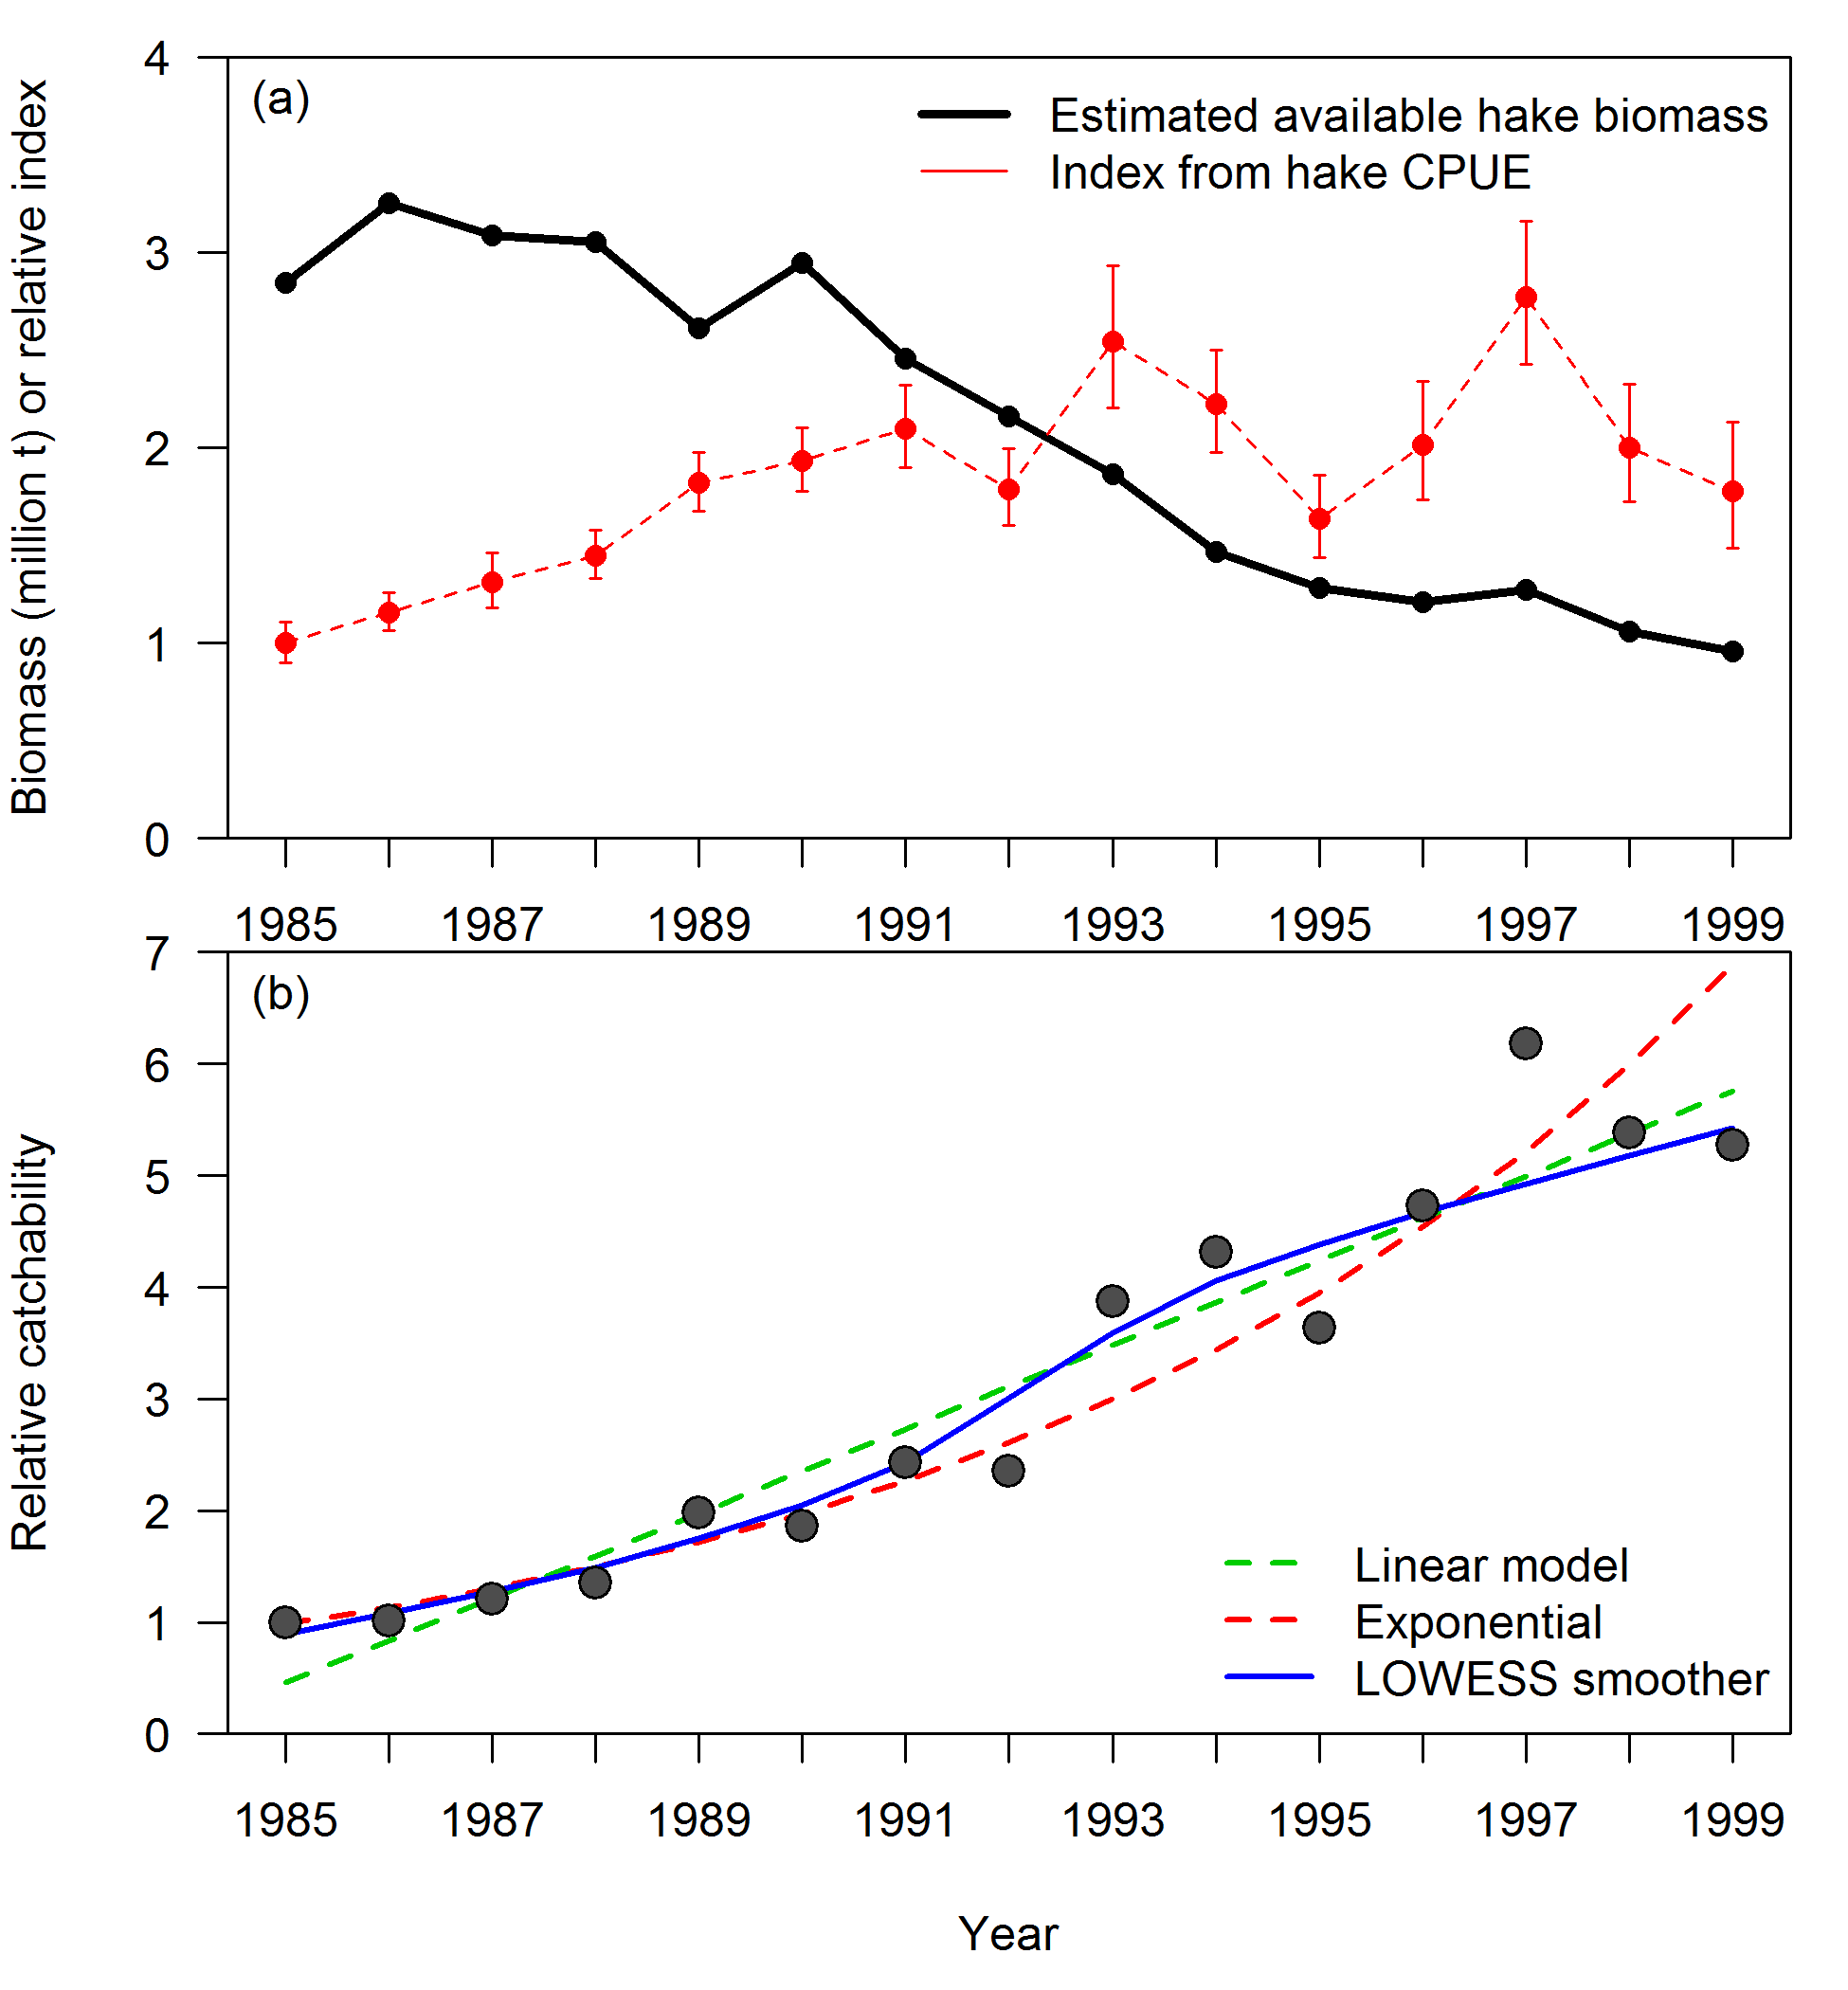
\includegraphics{Figures/ASHOP_catchability_illustration.png}
\caption{Geostatical index for Pacific Hake developed using VAST
compared to the estimated avaialble hake biomass.\label{fig:ASHOP_X3}}
\end{figure}

\begin{figure}[htbp]
\centering
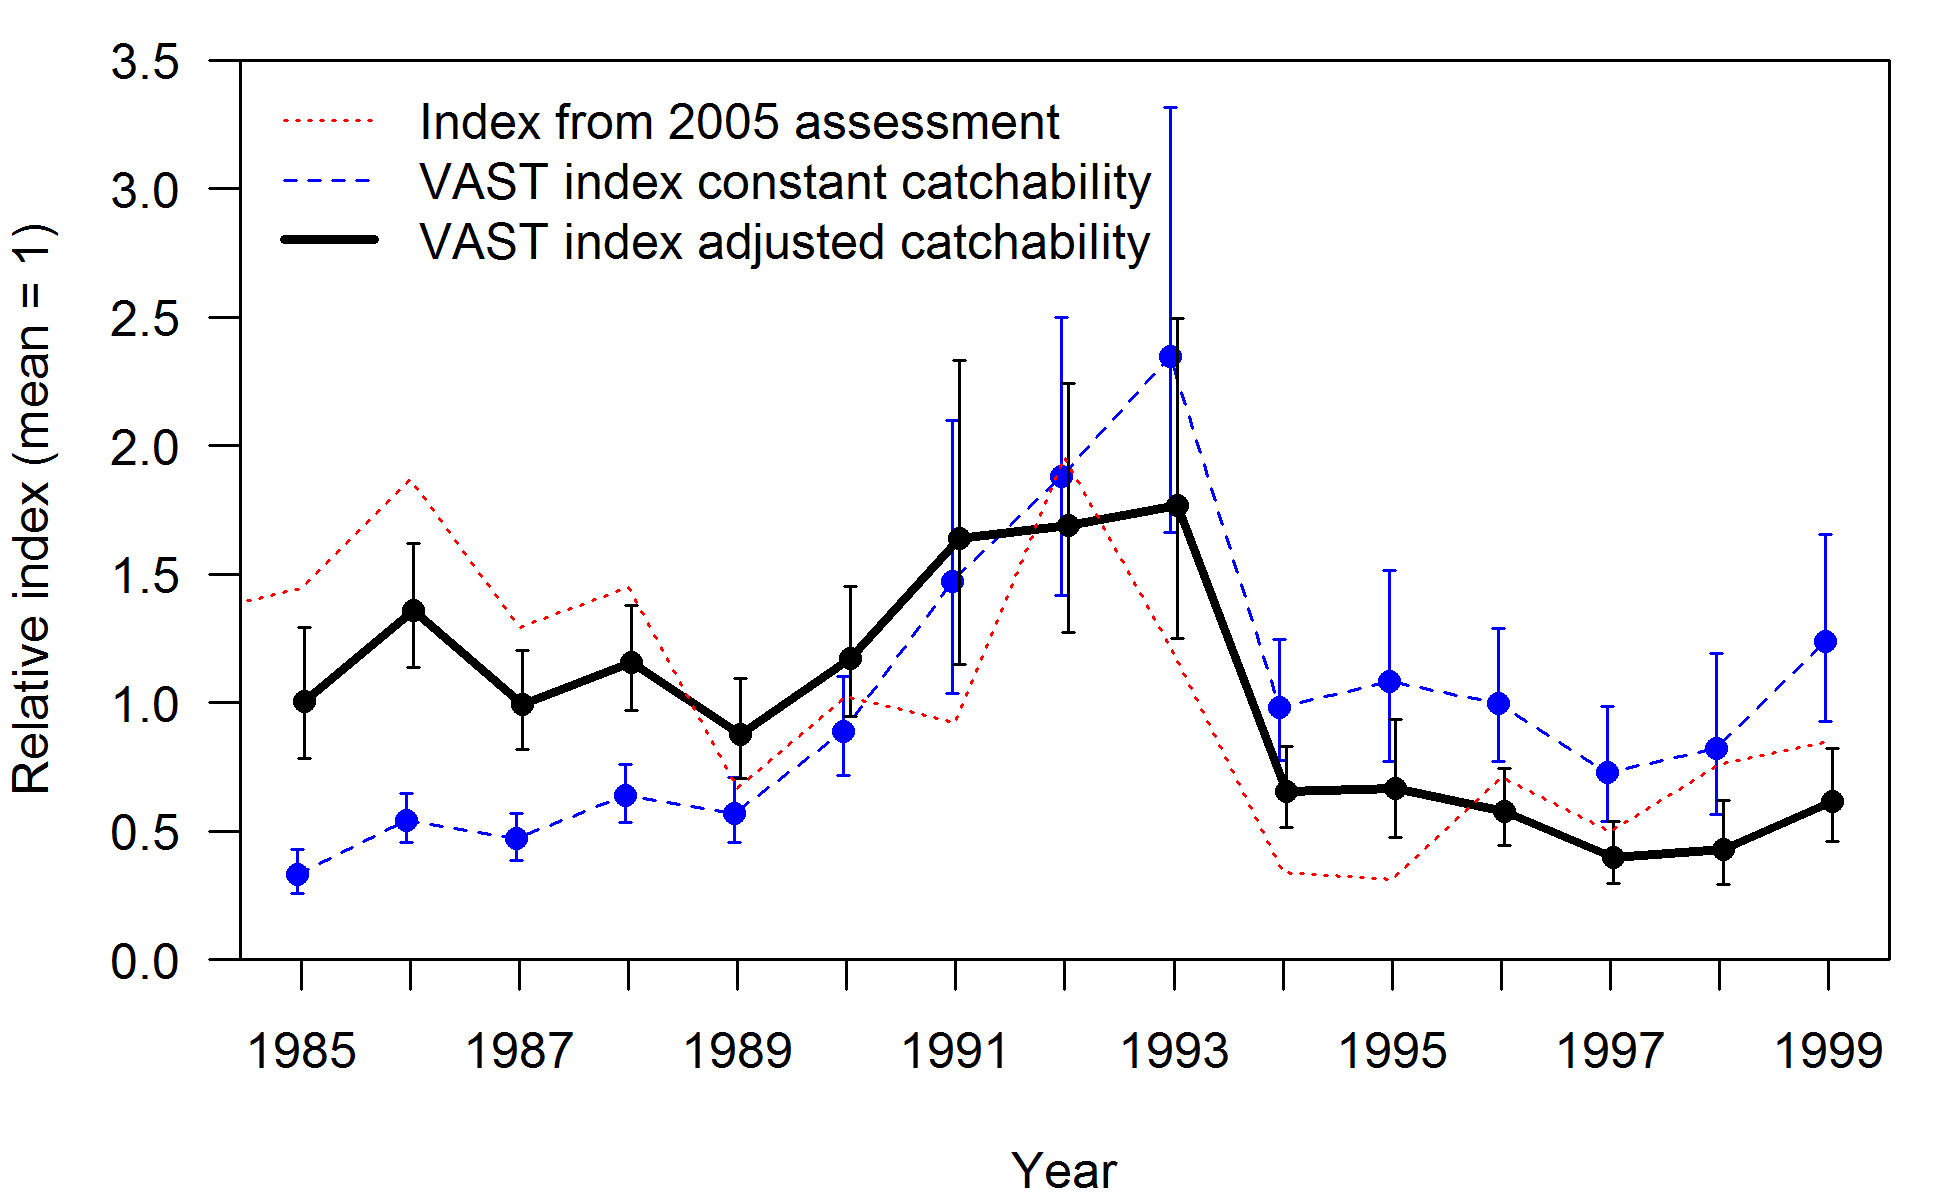
\includegraphics{Figures/ASHOP_index_illustration.png}
\caption{Index from the geostatistical model VAST with constant
catchability and adjusted for the estimated increase in catchability
(previous figure). These are compared to the index from the most recent
yellowtail assessment (Wallace and Lai, 2005).\label{fig:ASHOP_X4}}
\end{figure}

\FloatBarrier

\newpage

\subsubsection{Fits to indices of abundance for Northern
model}\label{fits-to-indices-of-abundance-for-northern-model}

\begin{figure}[htbp]
\centering
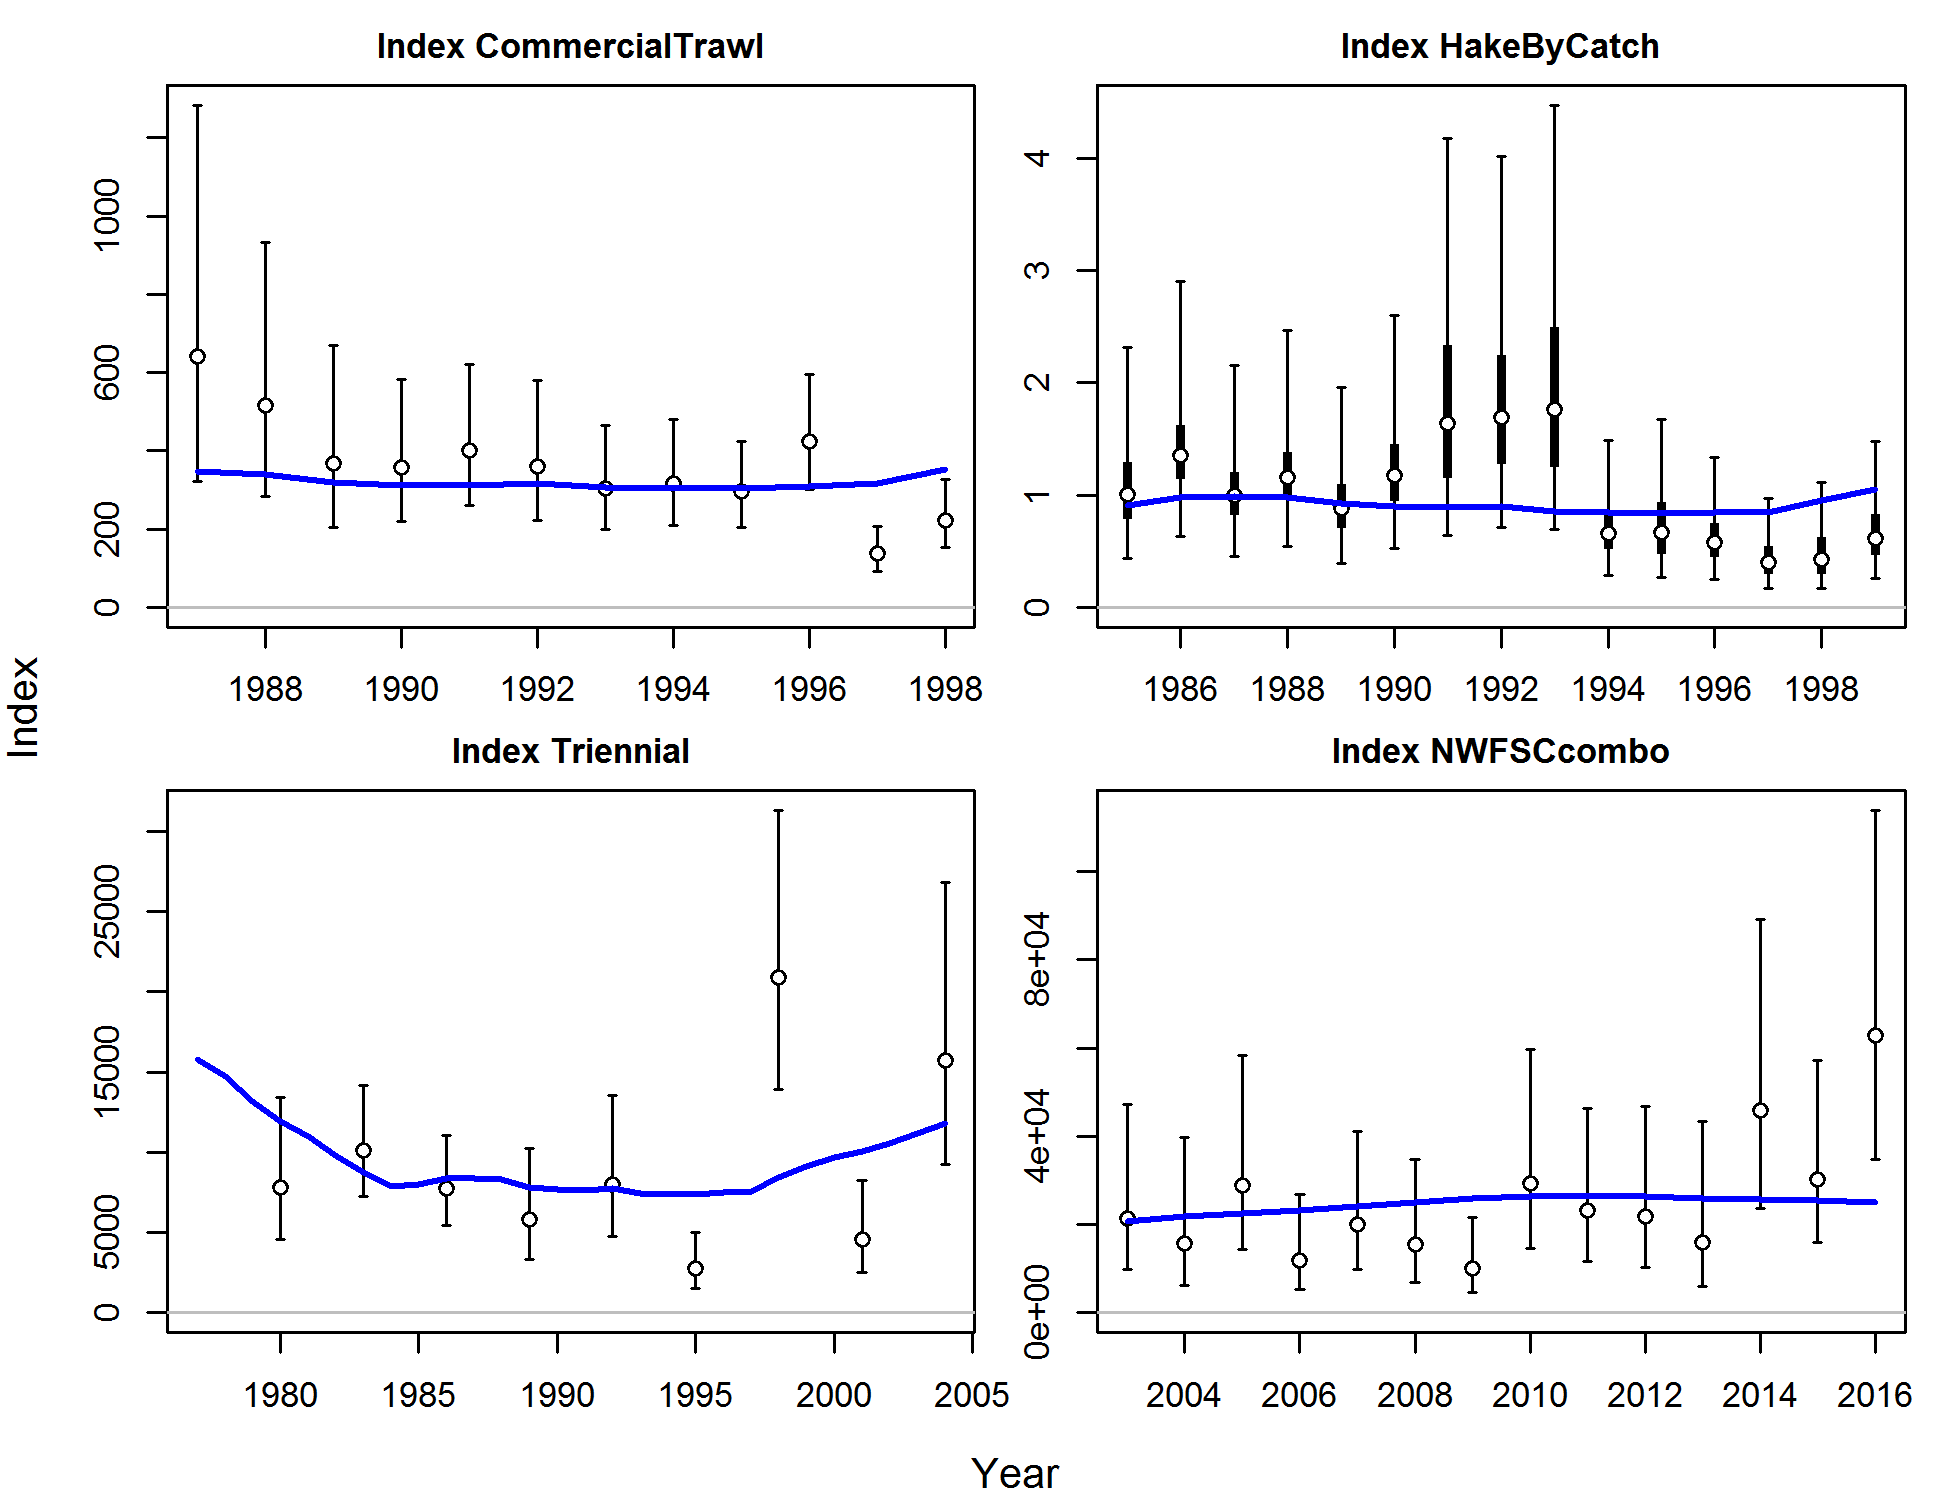
\includegraphics{r4ss/plots_mod1/index0_all_indices_fit.png}
\caption{Estimated fits to the CPUE and survey indices for the Northern
model. \label{fig:index_fits1}}
\end{figure}

\FloatBarrier

\newpage

\subsubsection{Length compositions for Northern
model}\label{length-compositions-for-northern-model}

\begin{figure}[htbp]
\centering
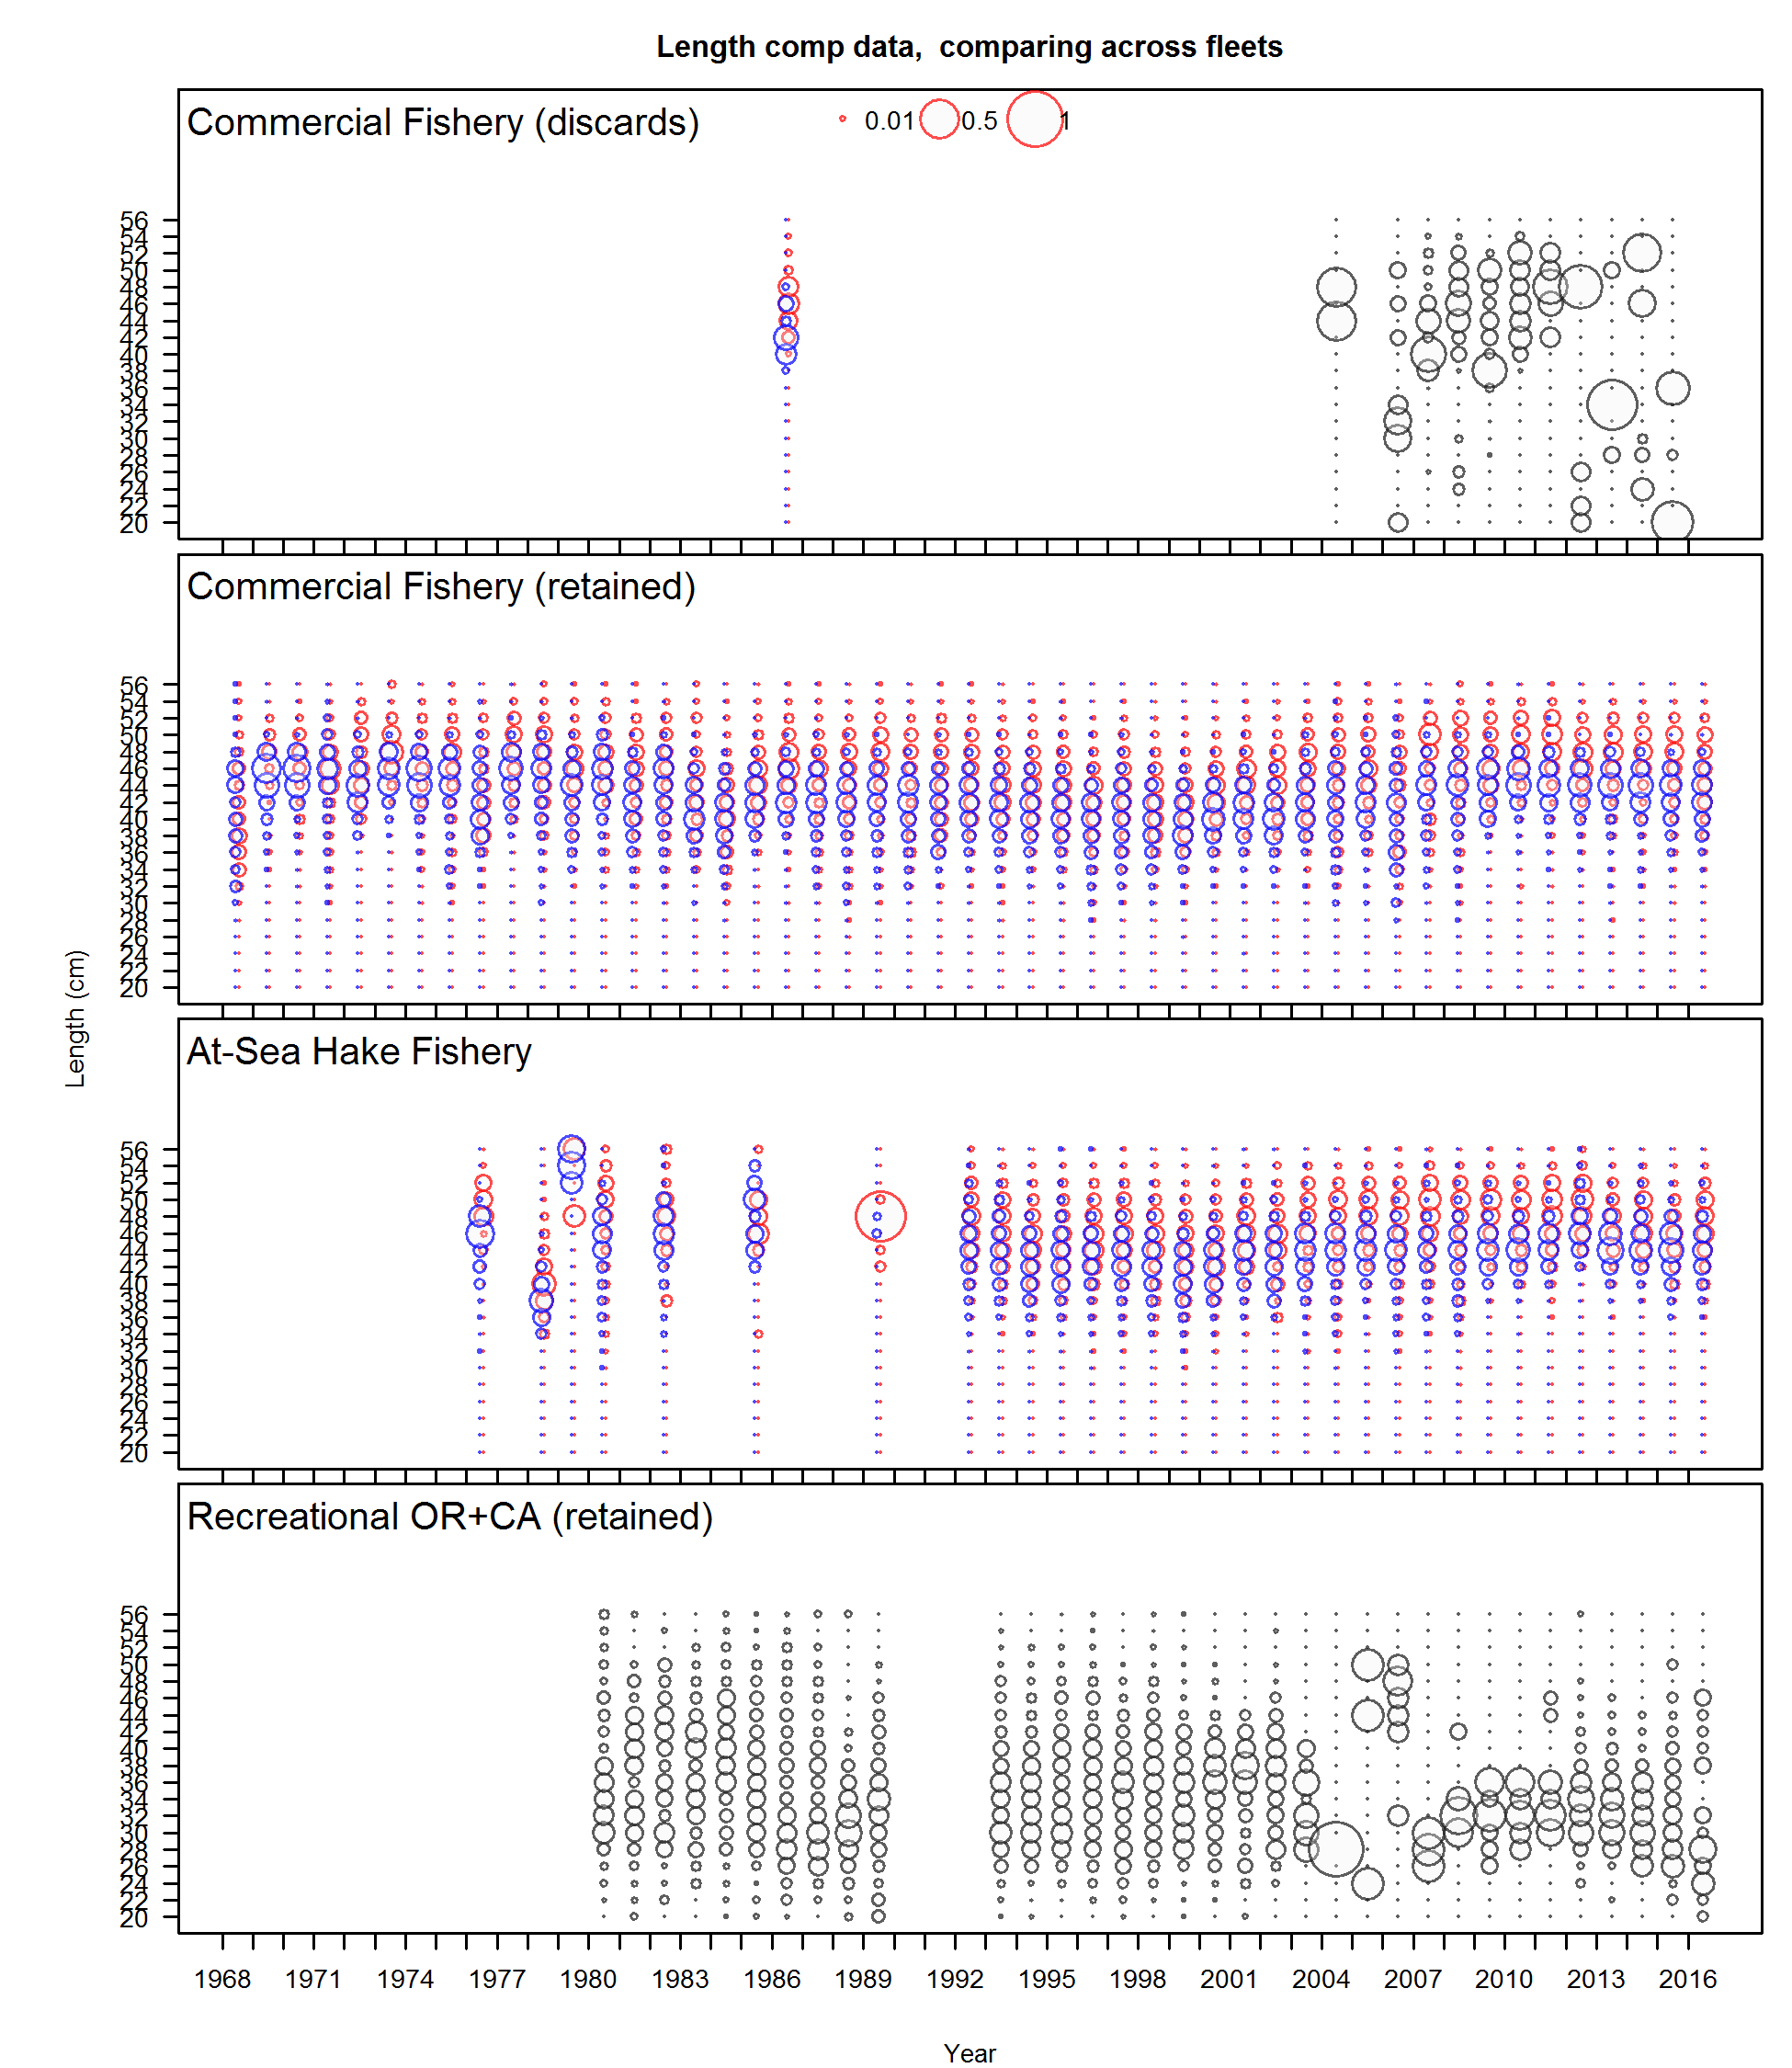
\includegraphics{r4ss/plots_mod1/comp_lendat__page1_multi-fleet_comparison.png}
\caption{Length compositions for all fleets in the Northern model
(figure 1 of 2). Bubble size is proportional to proportions within each
year. Bubble colors indicate unsexed fish (gray), females (red), and
males (blue).\label{fig:comp_length_bubble_mod1_page1}}
\end{figure}

\begin{figure}[htbp]
\centering
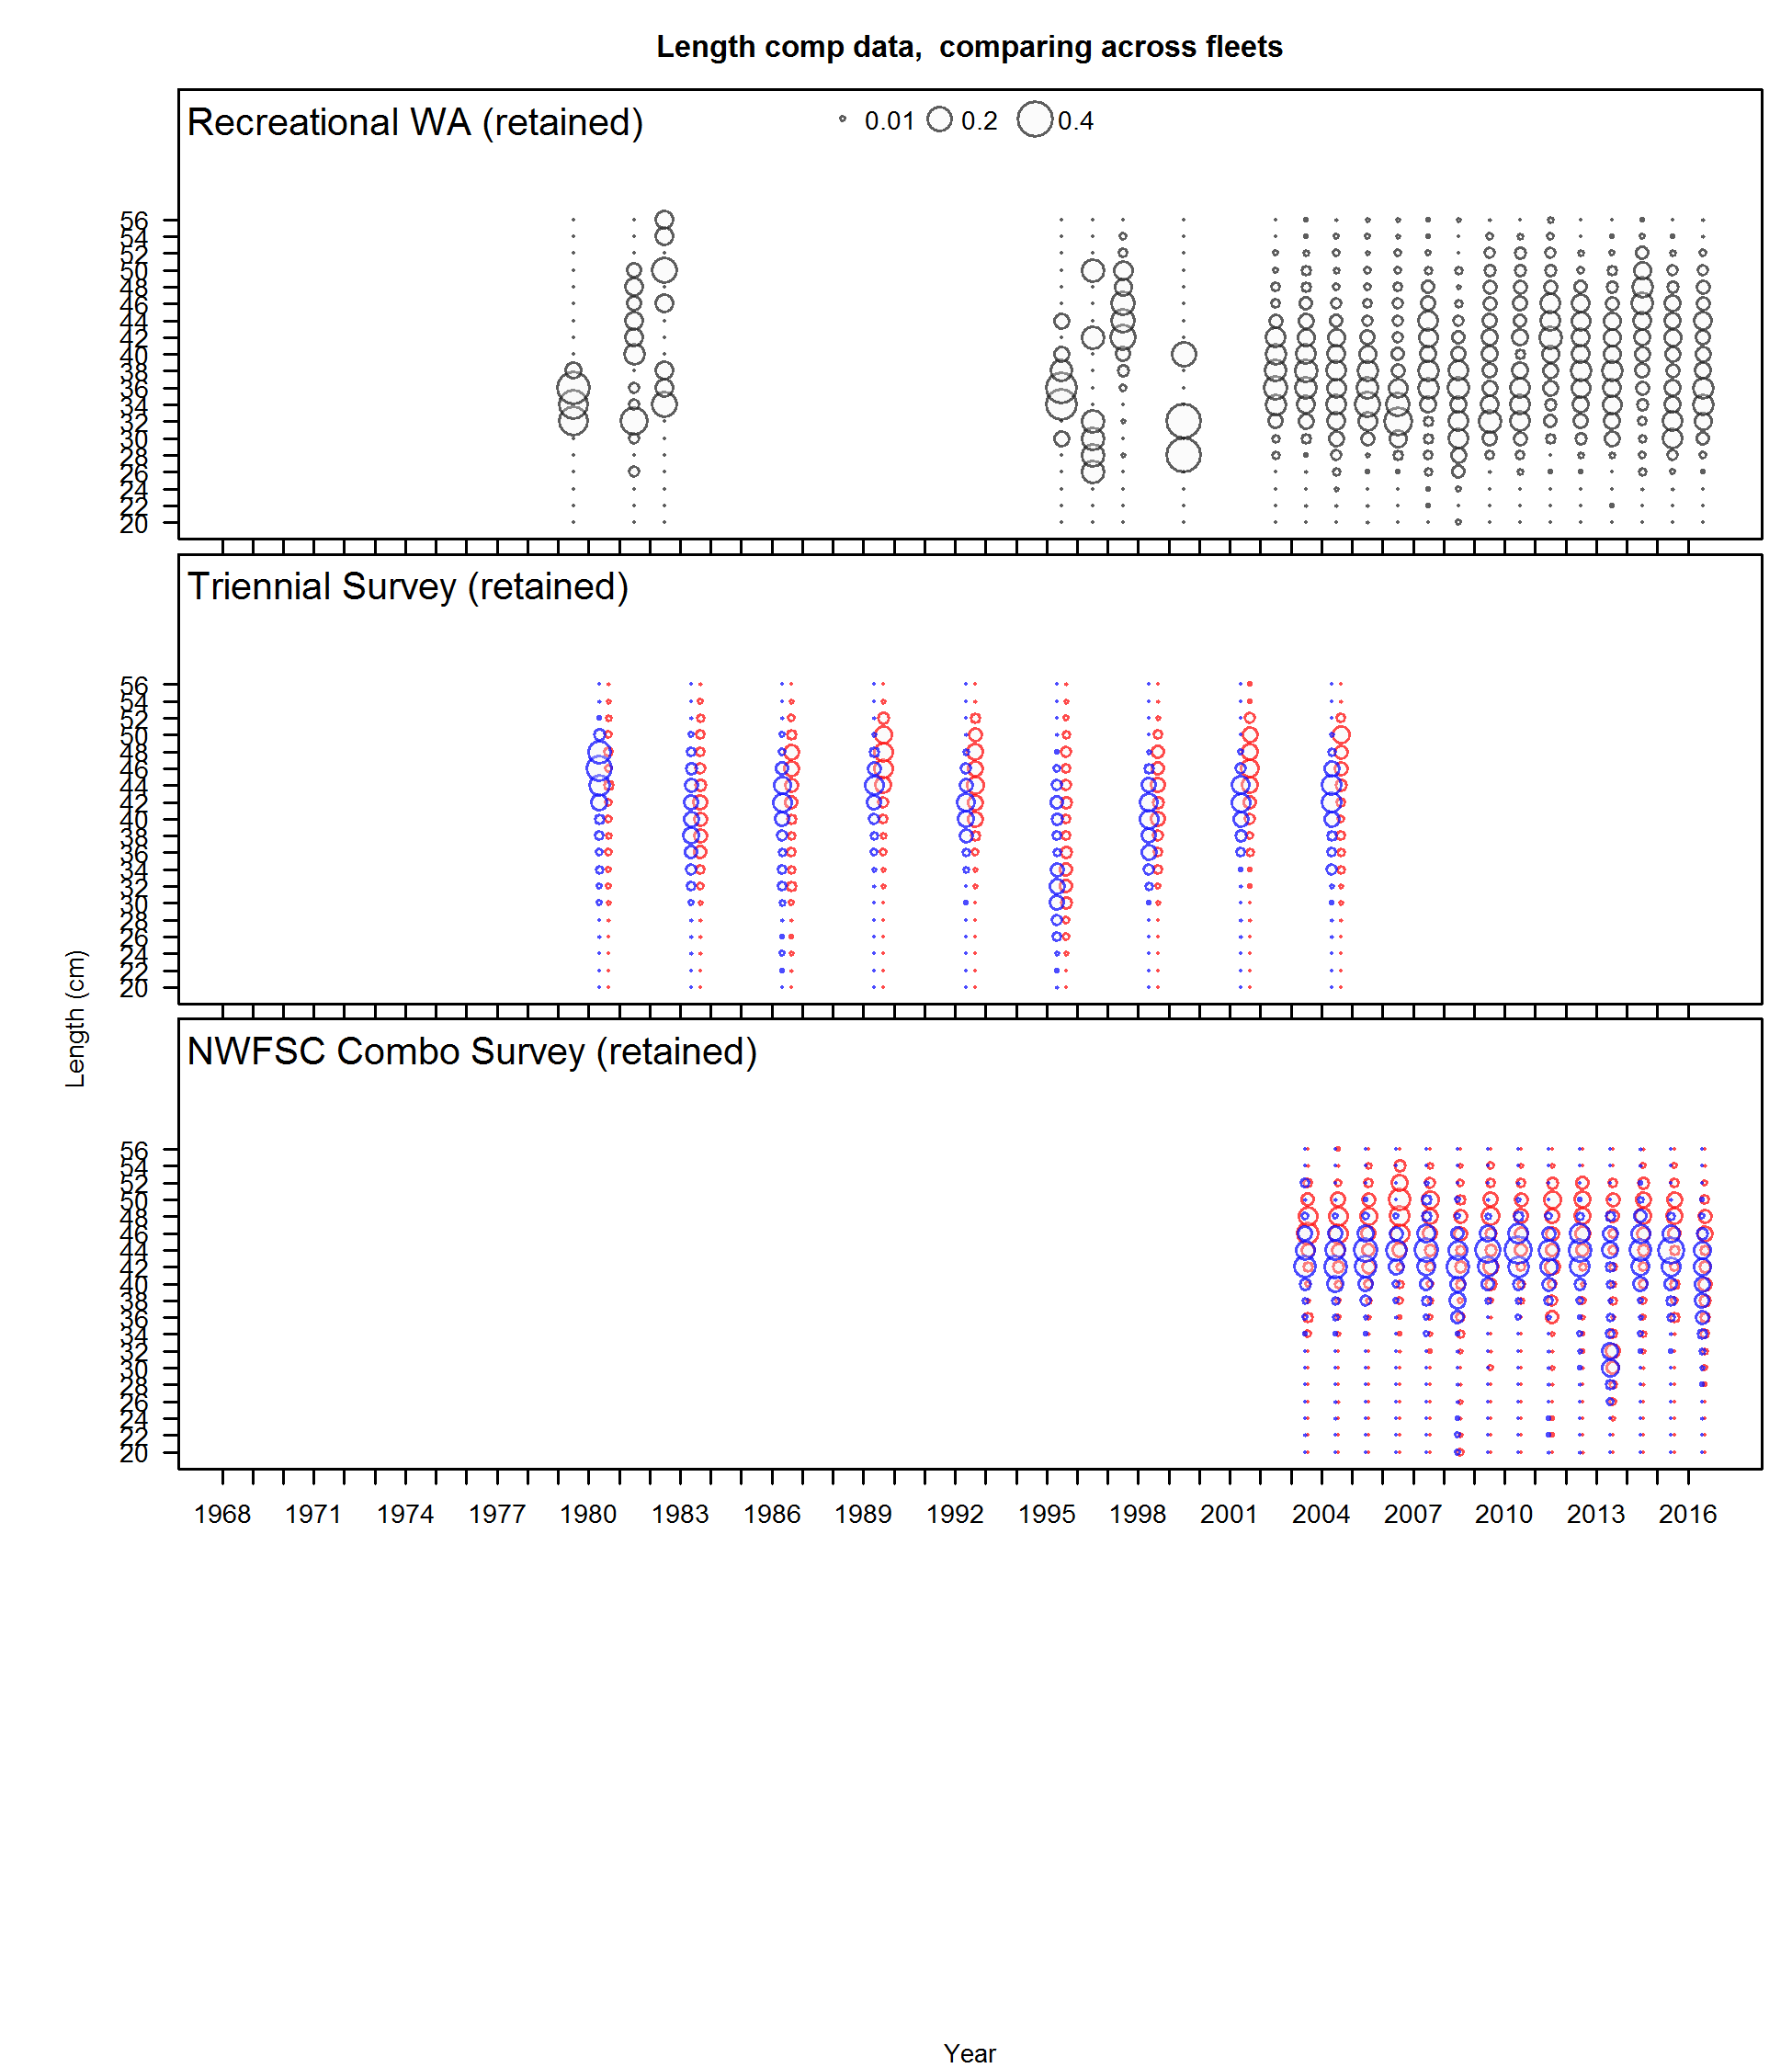
\includegraphics{r4ss/plots_mod1/comp_lendat__page2_multi-fleet_comparison.png}
\caption{Length compositions for all fleets in the Northern model
(figure 2 of 2). \label{fig:comp_length_bubble_mod1_page2}}
\end{figure}

\FloatBarrier

\newpage

\begin{figure}[htbp]
\centering
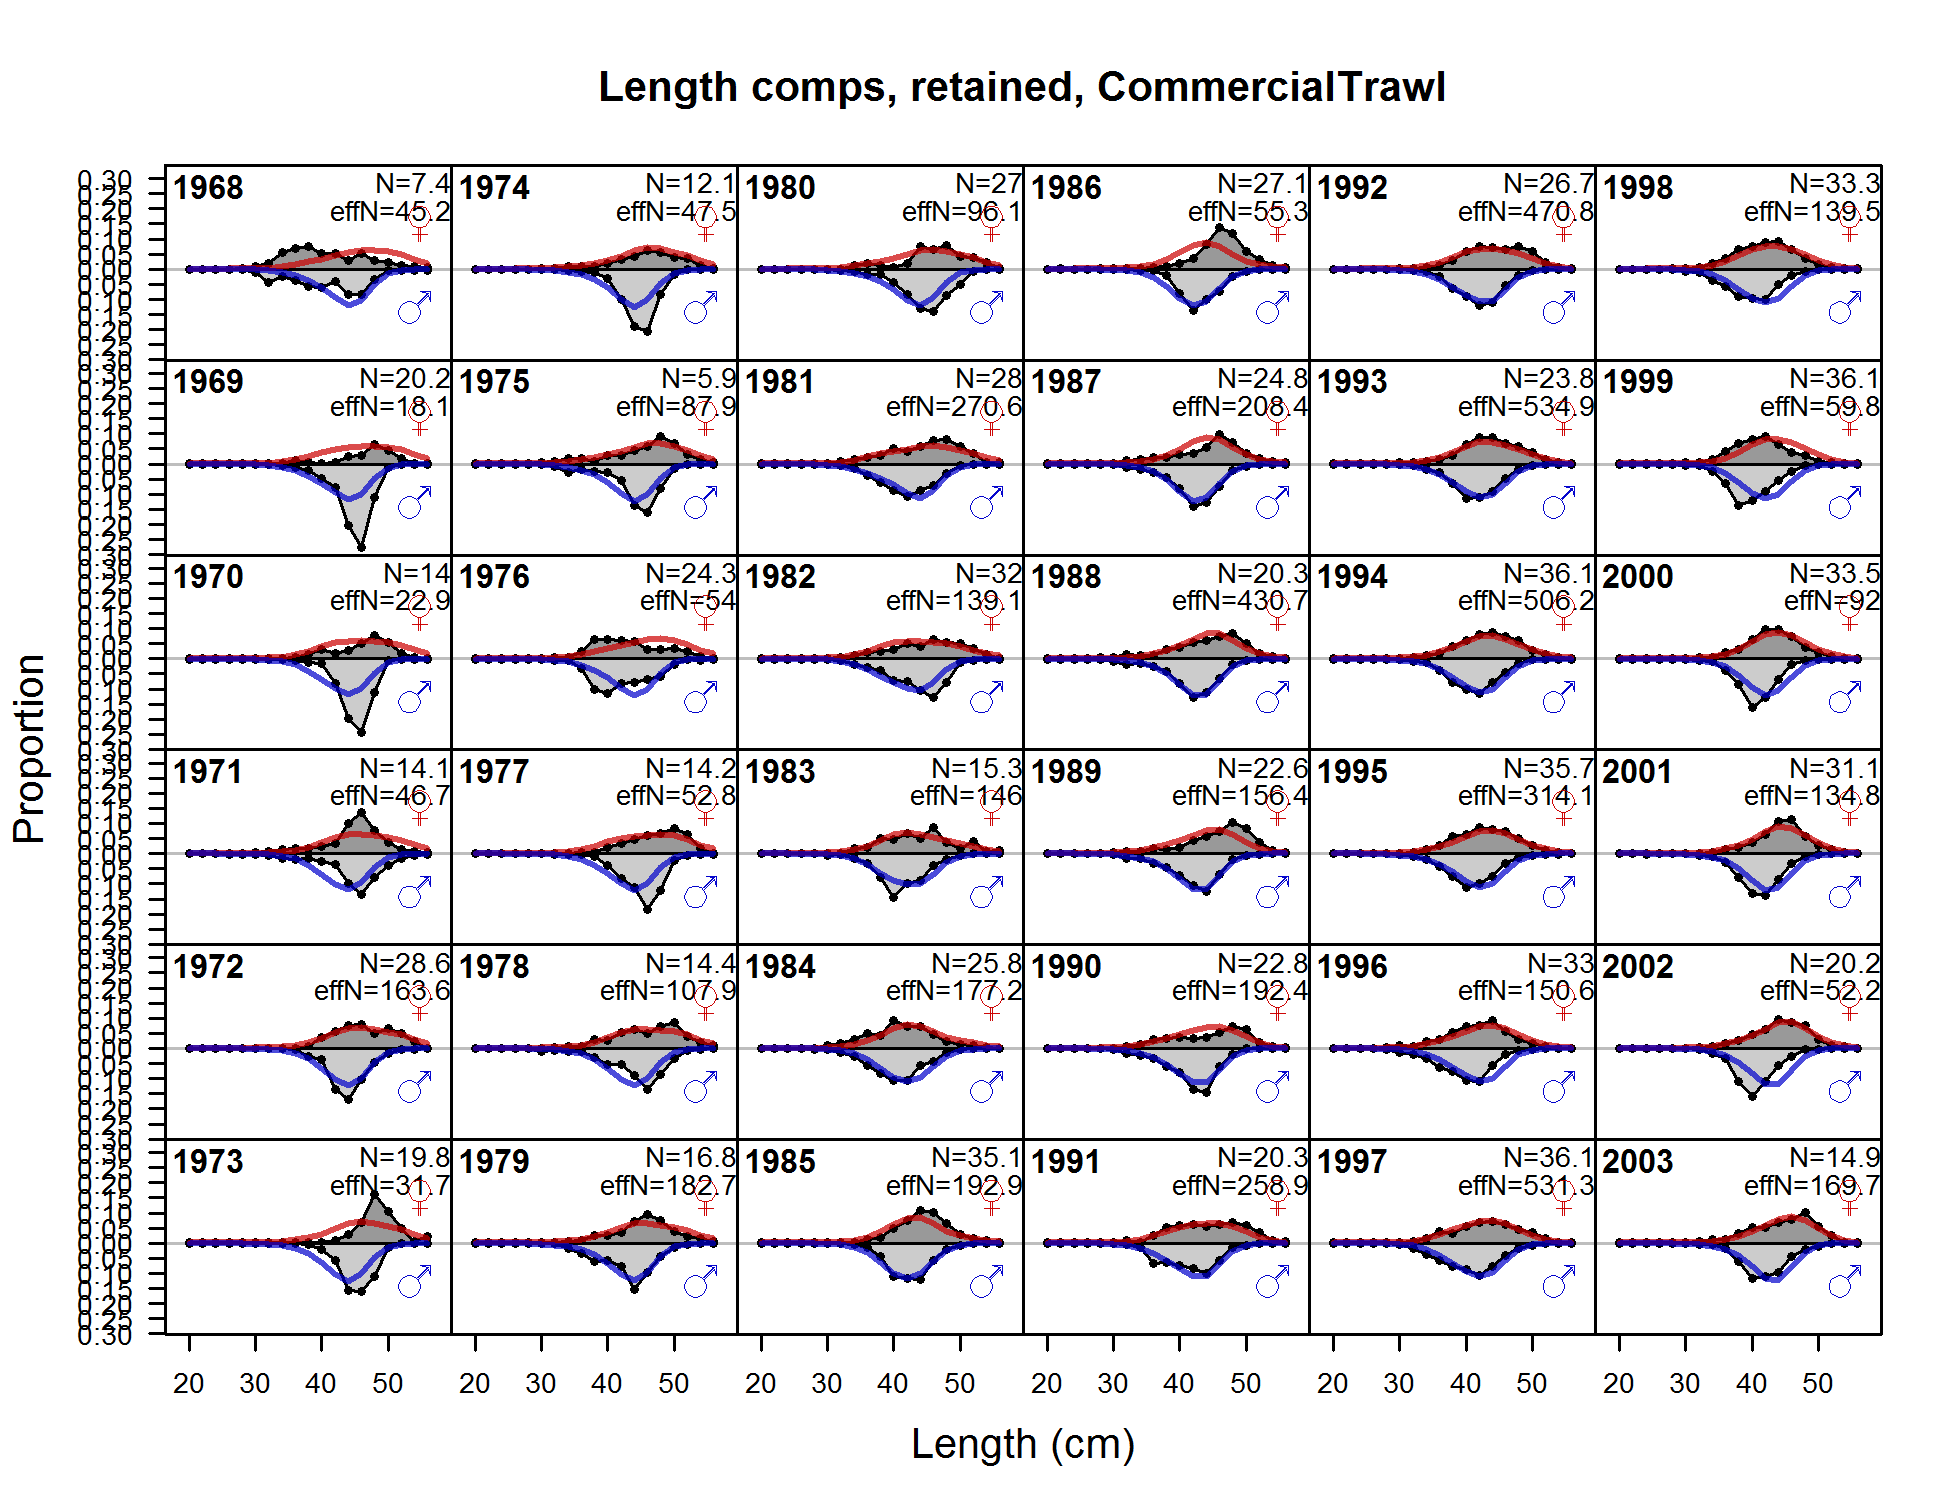
\includegraphics{./r4ss/plots_mod1/comp_lenfit_flt1mkt2_page1.png}
\caption{\textbf{Northern model} Length comps, retained, Commercial
Fishery (plot 1 of 2) \label{fig:mod1_1_comp_lenfit_flt1mkt2_page1}}
\end{figure}

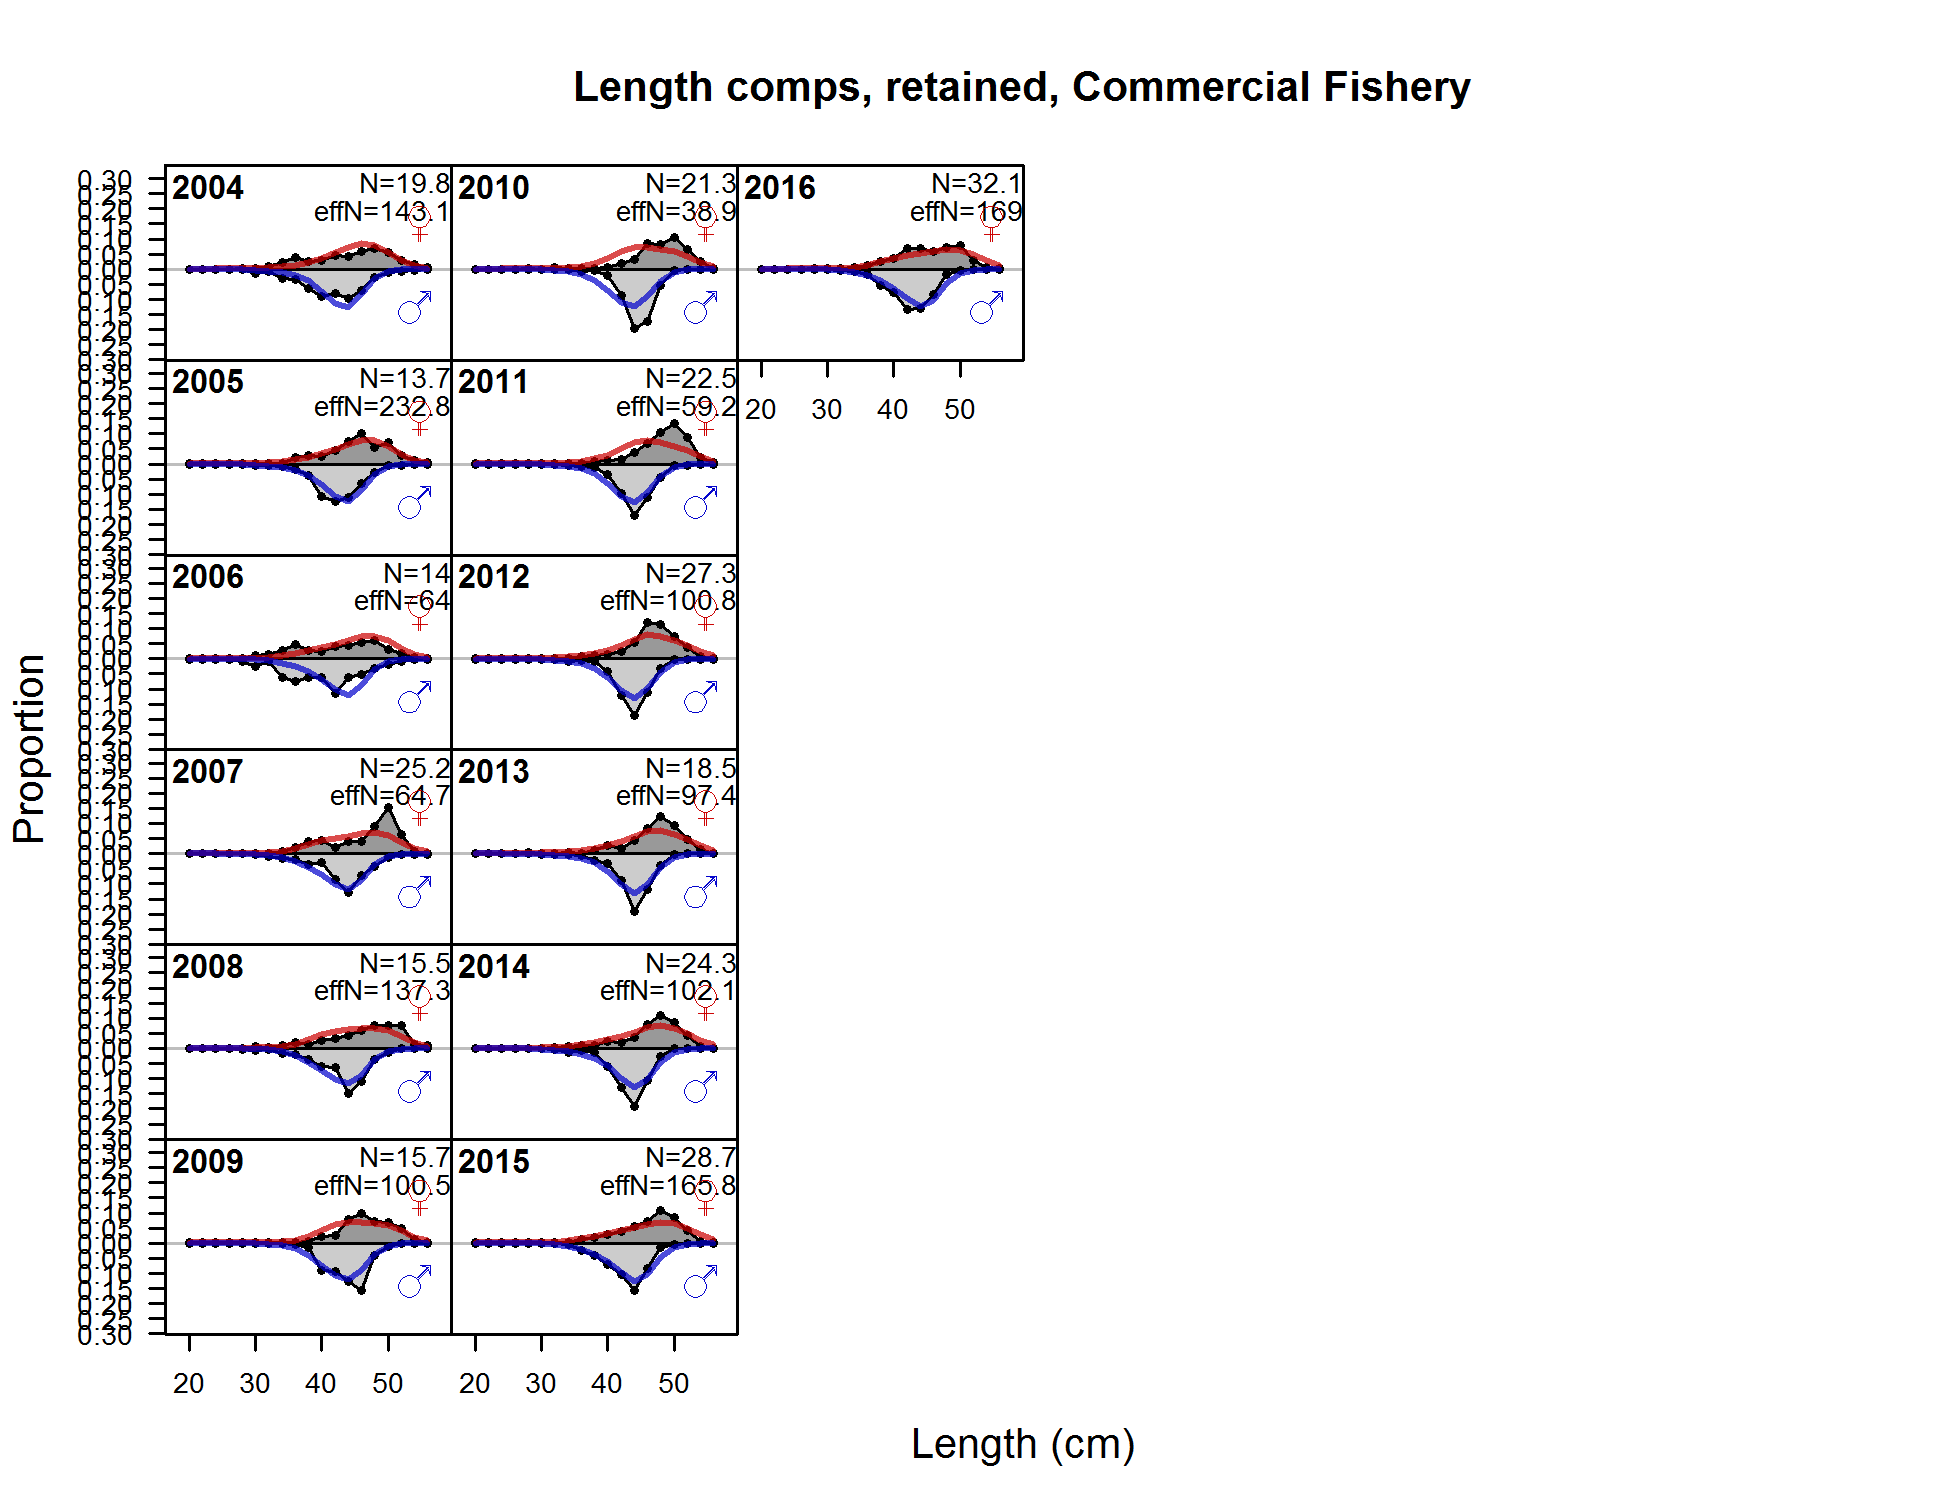
\includegraphics{./r4ss/plots_mod1/comp_lenfit_flt1mkt2_page2.png}

\begin{center} 

            Figure continued from previous page 

            \end{center}

\begin{figure}[htbp]
\centering
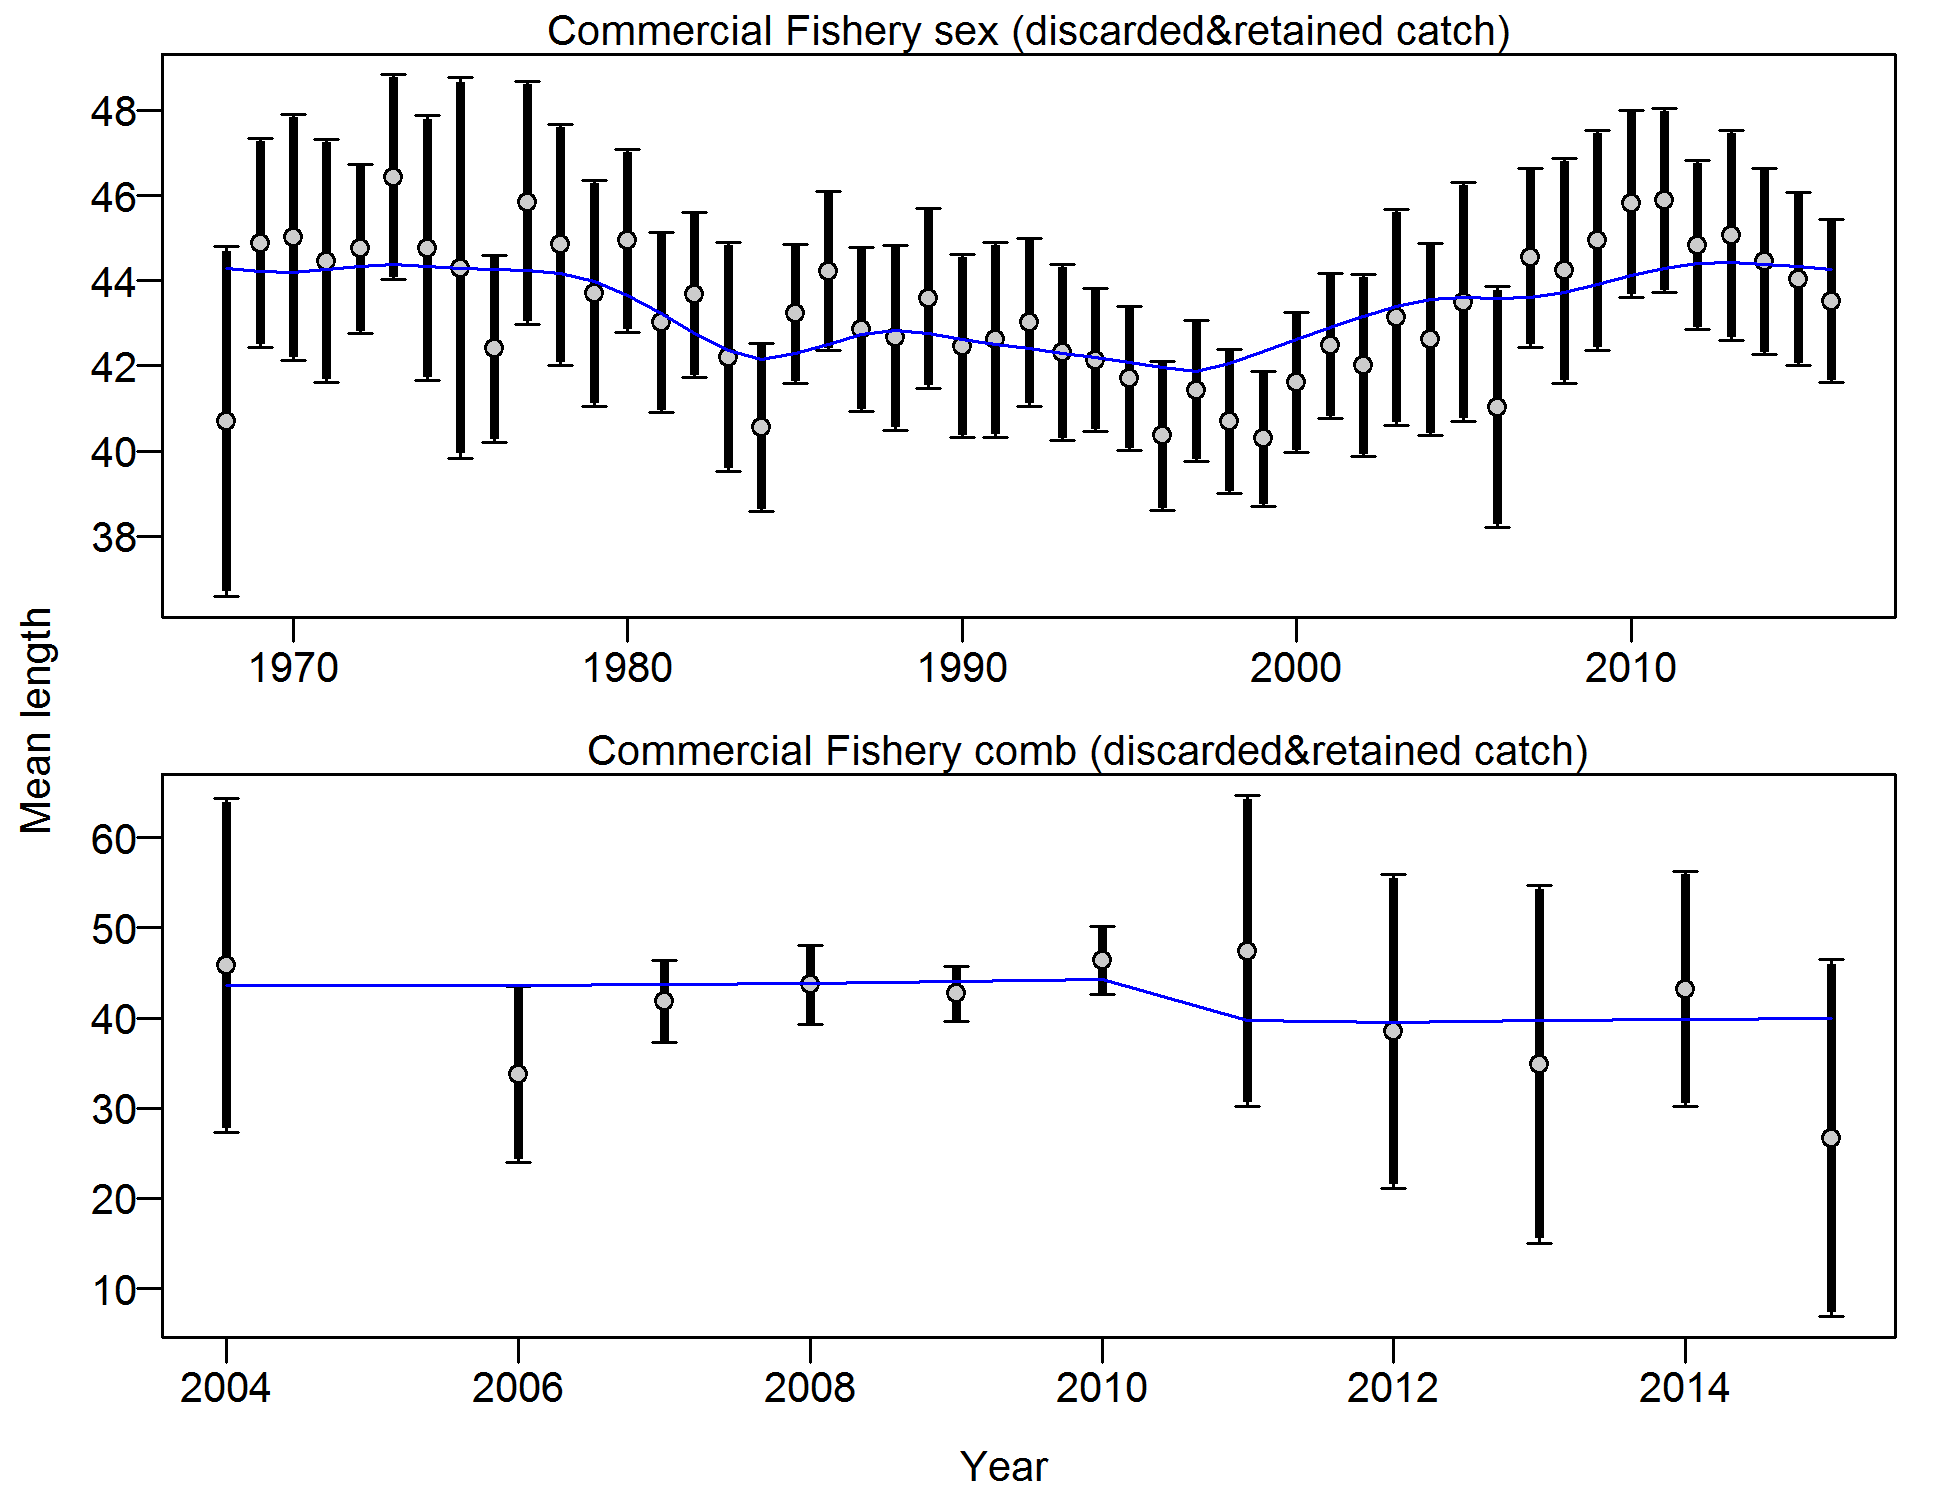
\includegraphics{./r4ss/plots_mod1/comp_lenfit_data_weighting_TA1.8_Commercial Fishery.png}
\caption{\textbf{Northern model} Mean length for Commercial Fishery with
95\% confidence intervals based on current samples sizes. Francis data
weighting method TA1.8: thinner intervals (with capped ends) show result
of further adjusting sample sizes based on suggested multiplier (with
95\% interval) for len data from Commercial Fishery: 0.9821
(0.7428\_1.4551) For more info, see Francis, R.I.C.C. (2011). Data
weighting in statistical fisheries stock assessment models. Can. J.
Fish. Aquat. Sci. 68: 1124\_1138.
\label{fig:mod1_5_comp_lenfit_data_weighting_TA1.8_Commercial Fishery}}
\end{figure}

\begin{figure}[htbp]
\centering
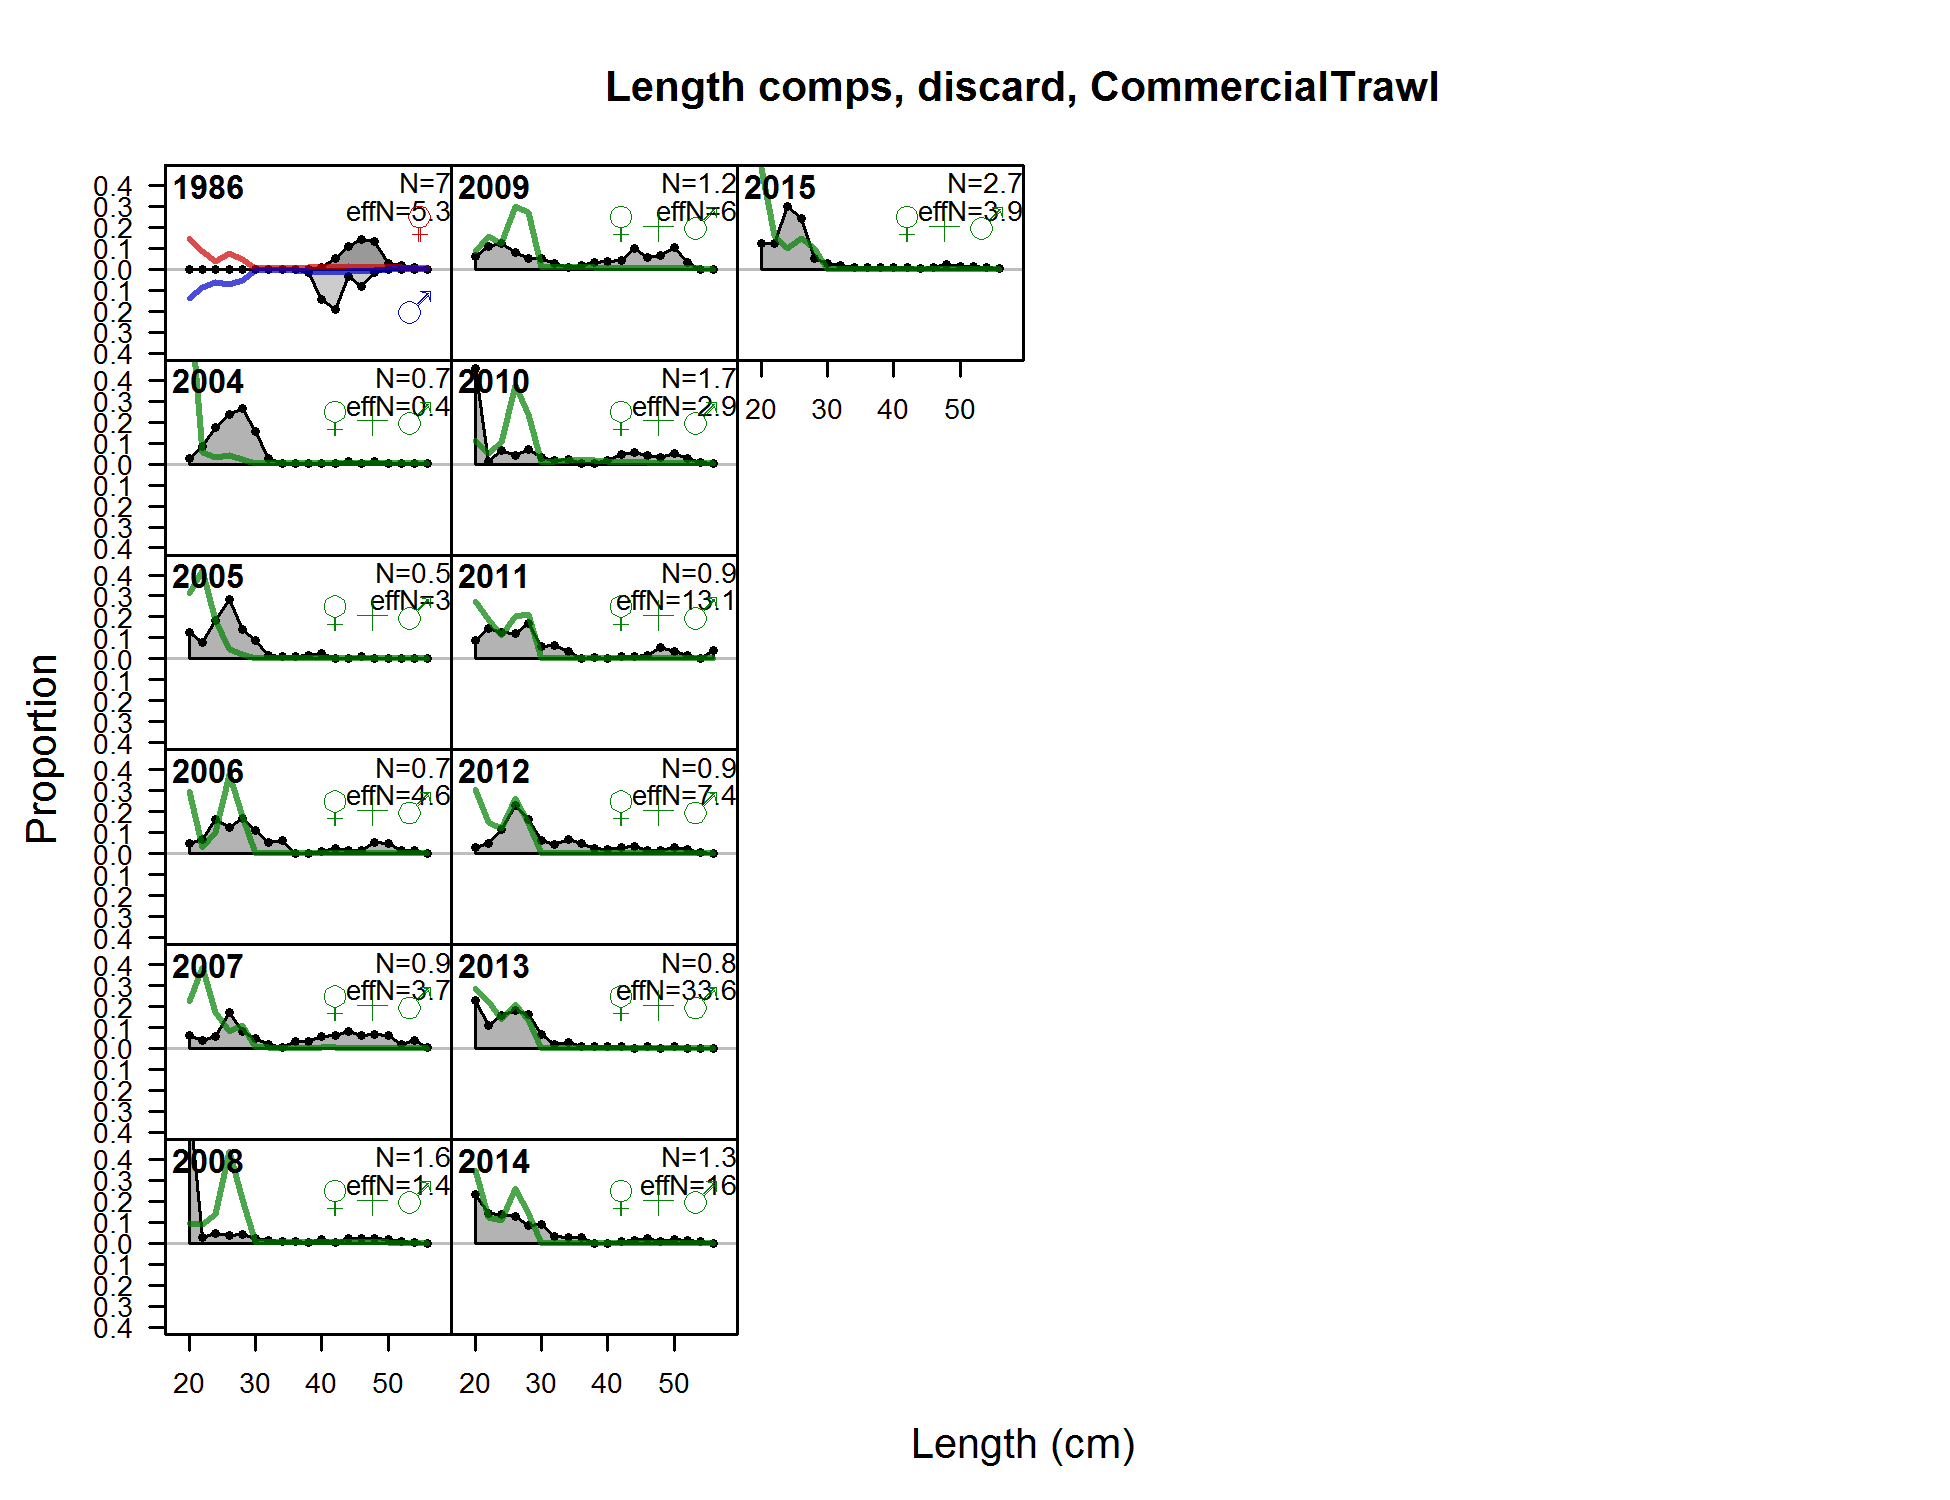
\includegraphics{./r4ss/plots_mod1/comp_lenfit_flt1mkt1.png}
\caption{\textbf{Northern model} Length comps, discard, Commercial
Fishery \label{fig:mod1_6_comp_lenfit_flt1mkt1}}
\end{figure}

\begin{figure}[htbp]
\centering
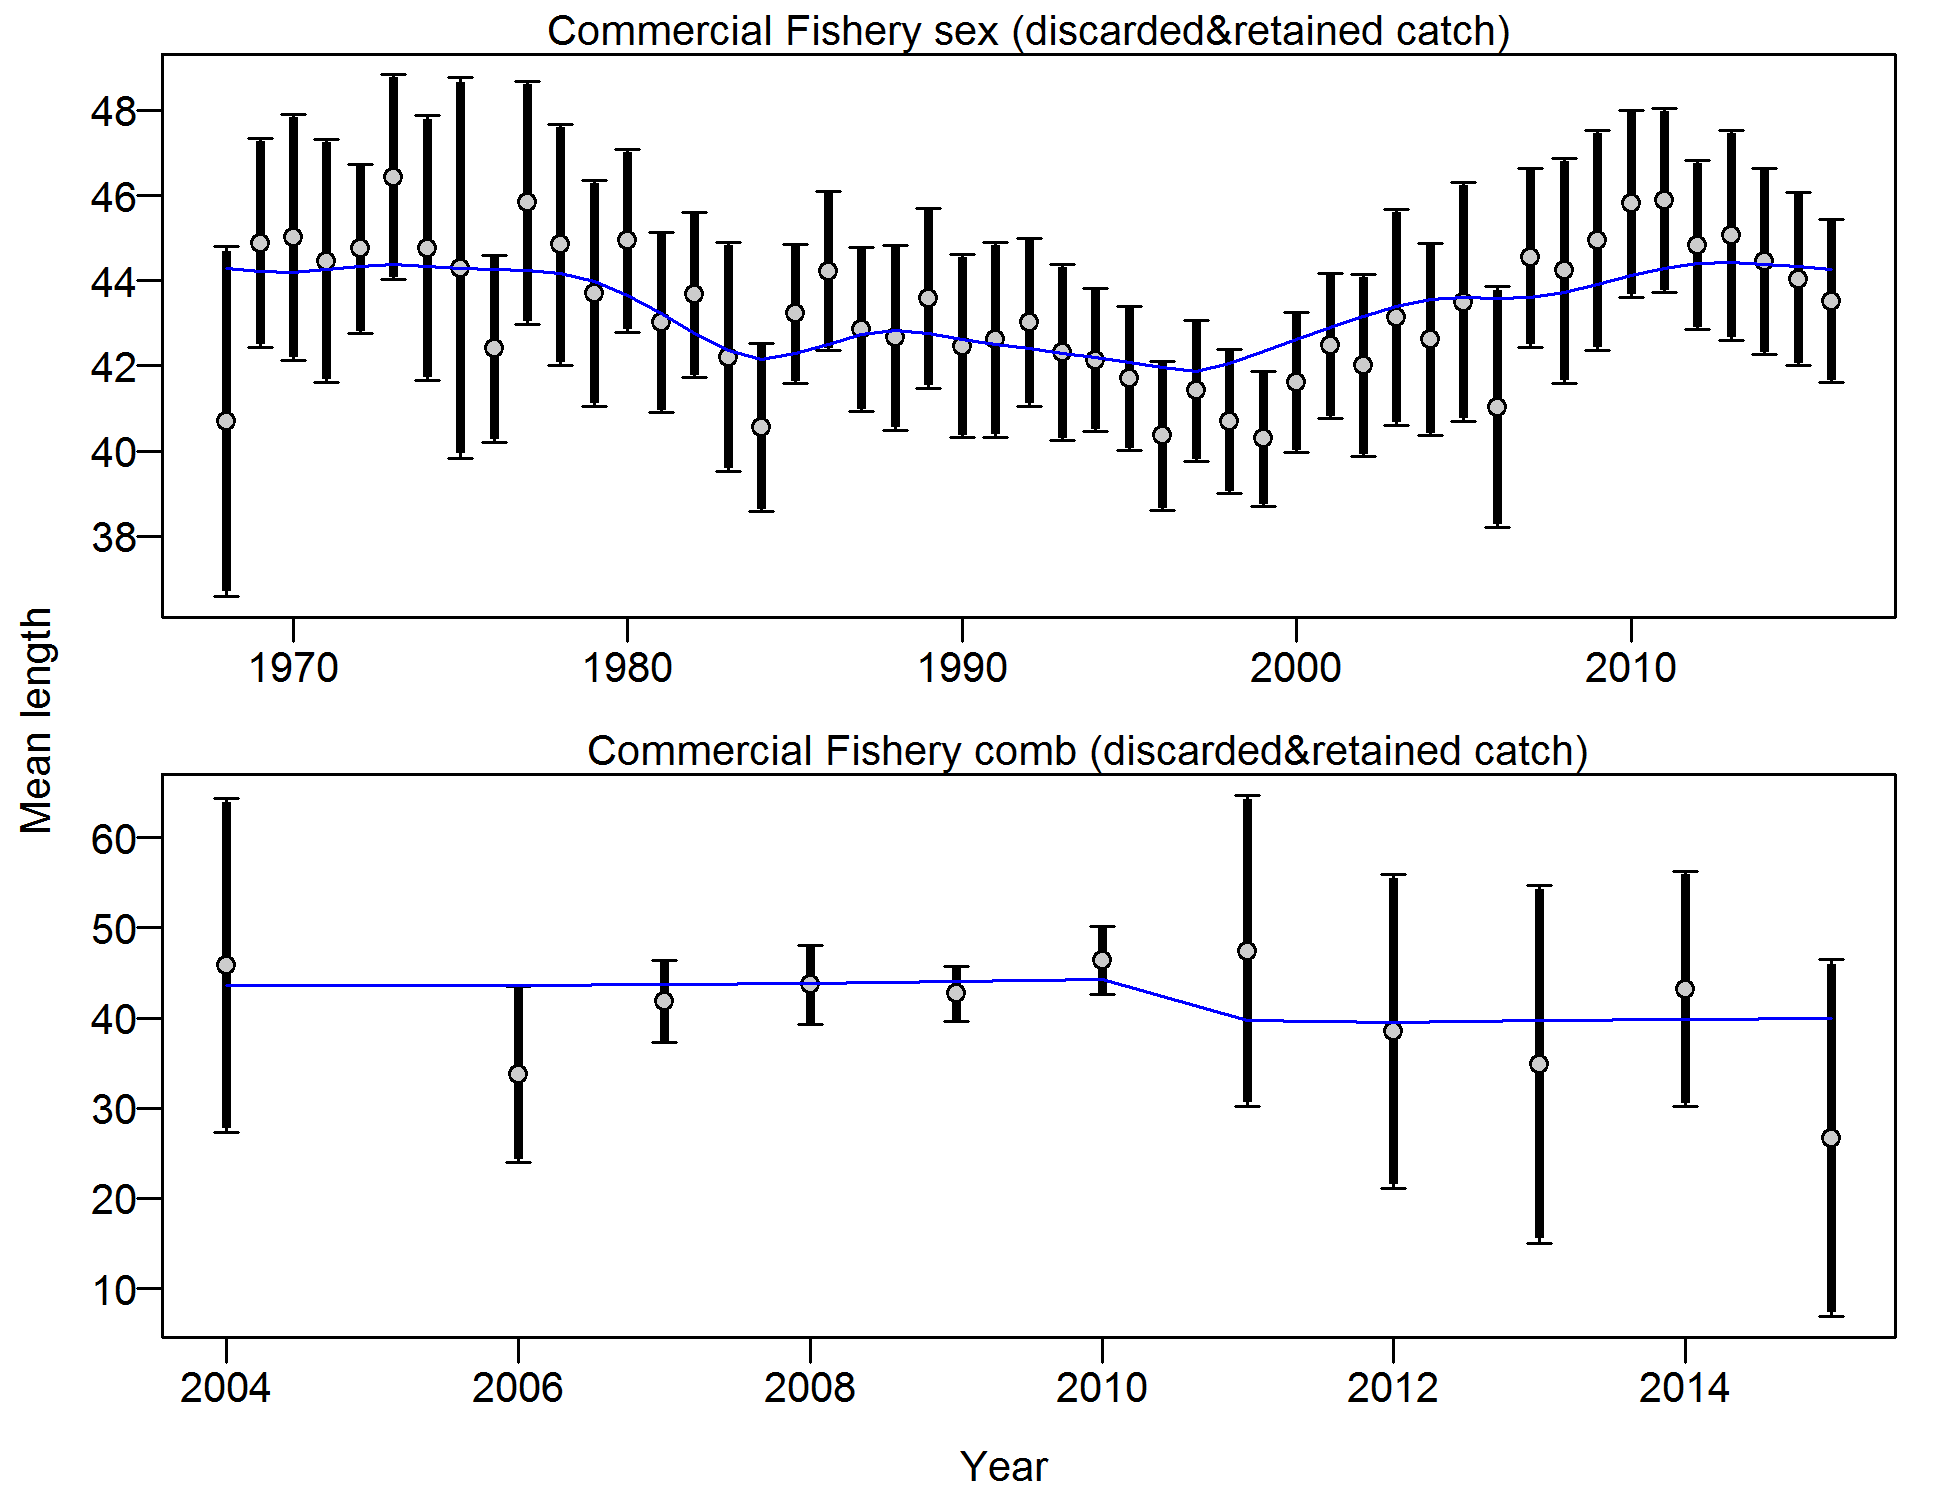
\includegraphics{./r4ss/plots_mod1/comp_lenfit_data_weighting_TA1.8_Commercial Fishery.png}
\caption{\textbf{Northern model} Mean length for Commercial Fishery with
95\% confidence intervals based on current samples sizes. Francis data
weighting method TA1.8: thinner intervals (with capped ends) show result
of further adjusting sample sizes based on suggested multiplier (with
95\% interval) for len data from Commercial Fishery: 0.9821
(0.7498\_1.4377) For more info, see Francis, R.I.C.C. (2011). Data
weighting in statistical fisheries stock assessment models. Can. J.
Fish. Aquat. Sci. 68: 1124\_1138.
\label{fig:mod1_9_comp_lenfit_data_weighting_TA1.8_Commercial Fishery}}
\end{figure}

\begin{figure}[htbp]
\centering
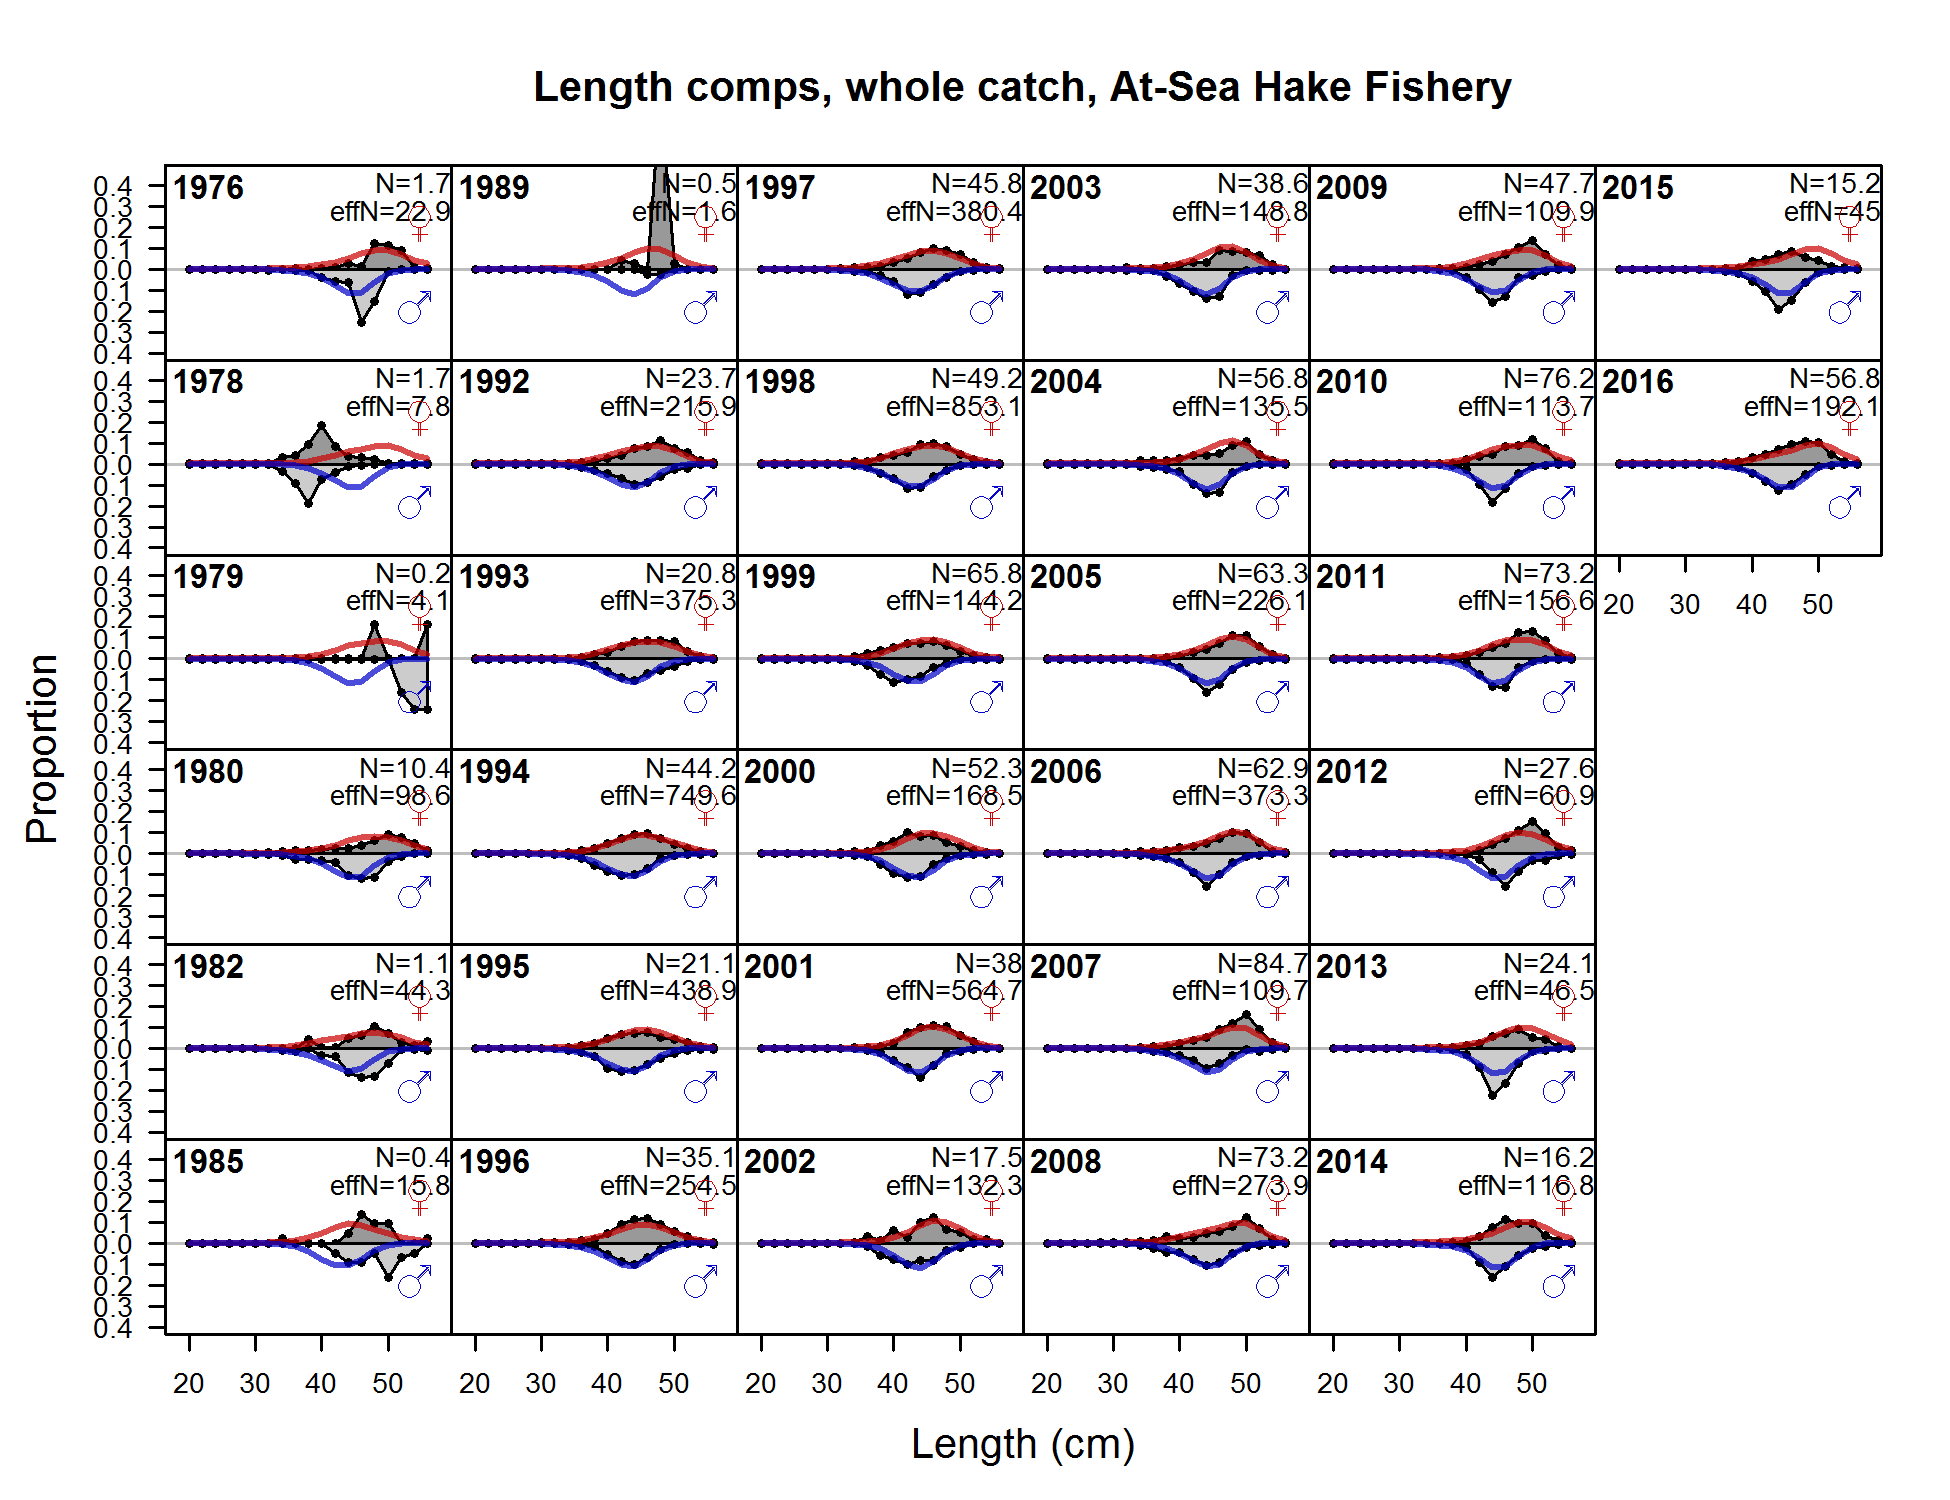
\includegraphics{./r4ss/plots_mod1/comp_lenfit_flt2mkt0.png}
\caption{\textbf{Northern model} Length comps, whole catch, At\_Sea Hake
Fishery \label{fig:mod1_10_comp_lenfit_flt2mkt0}}
\end{figure}

\begin{figure}[htbp]
\centering
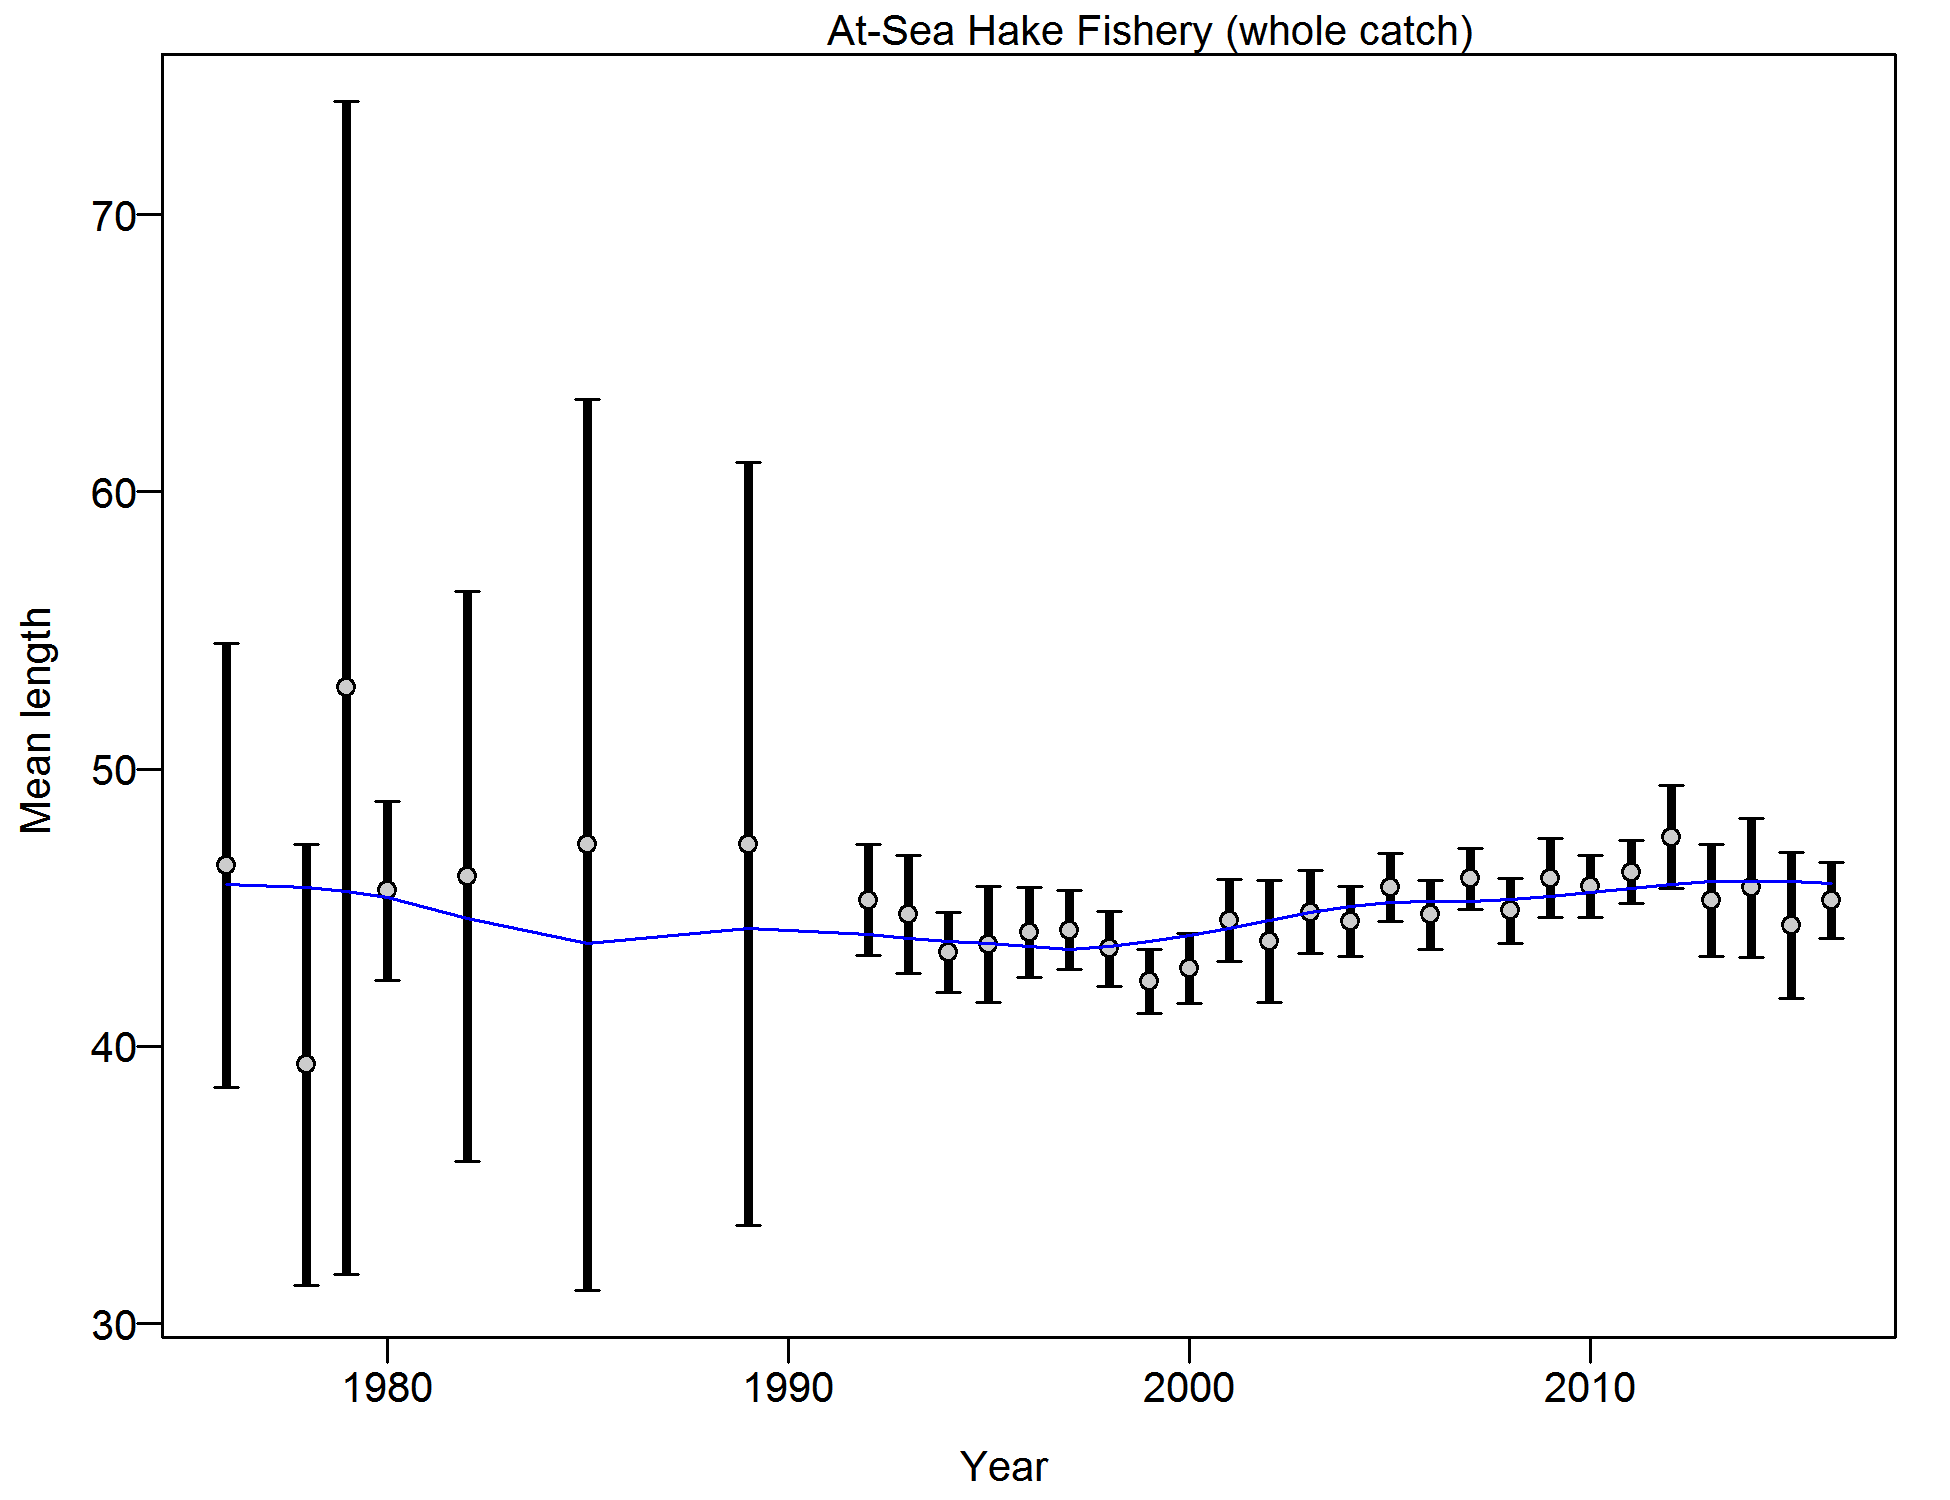
\includegraphics{./r4ss/plots_mod1/comp_lenfit_data_weighting_TA1.8_At-Sea Hake Fishery.png}
\caption{\textbf{Northern model} Mean length for At\_Sea Hake Fishery
with 95\% confidence intervals based on current samples sizes. Francis
data weighting method TA1.8: thinner intervals (with capped ends) show
result of further adjusting sample sizes based on suggested multiplier
(with 95\% interval) for len data from At\_Sea Hake Fishery: 0.9923
(0.6694\_1.8454) For more info, see Francis, R.I.C.C. (2011). Data
weighting in statistical fisheries stock assessment models. Can. J.
Fish. Aquat. Sci. 68: 1124\_1138.
\label{fig:mod1_13_comp_lenfit_data_weighting_TA1.8_At-Sea Hake Fishery}}
\end{figure}

\begin{figure}[htbp]
\centering
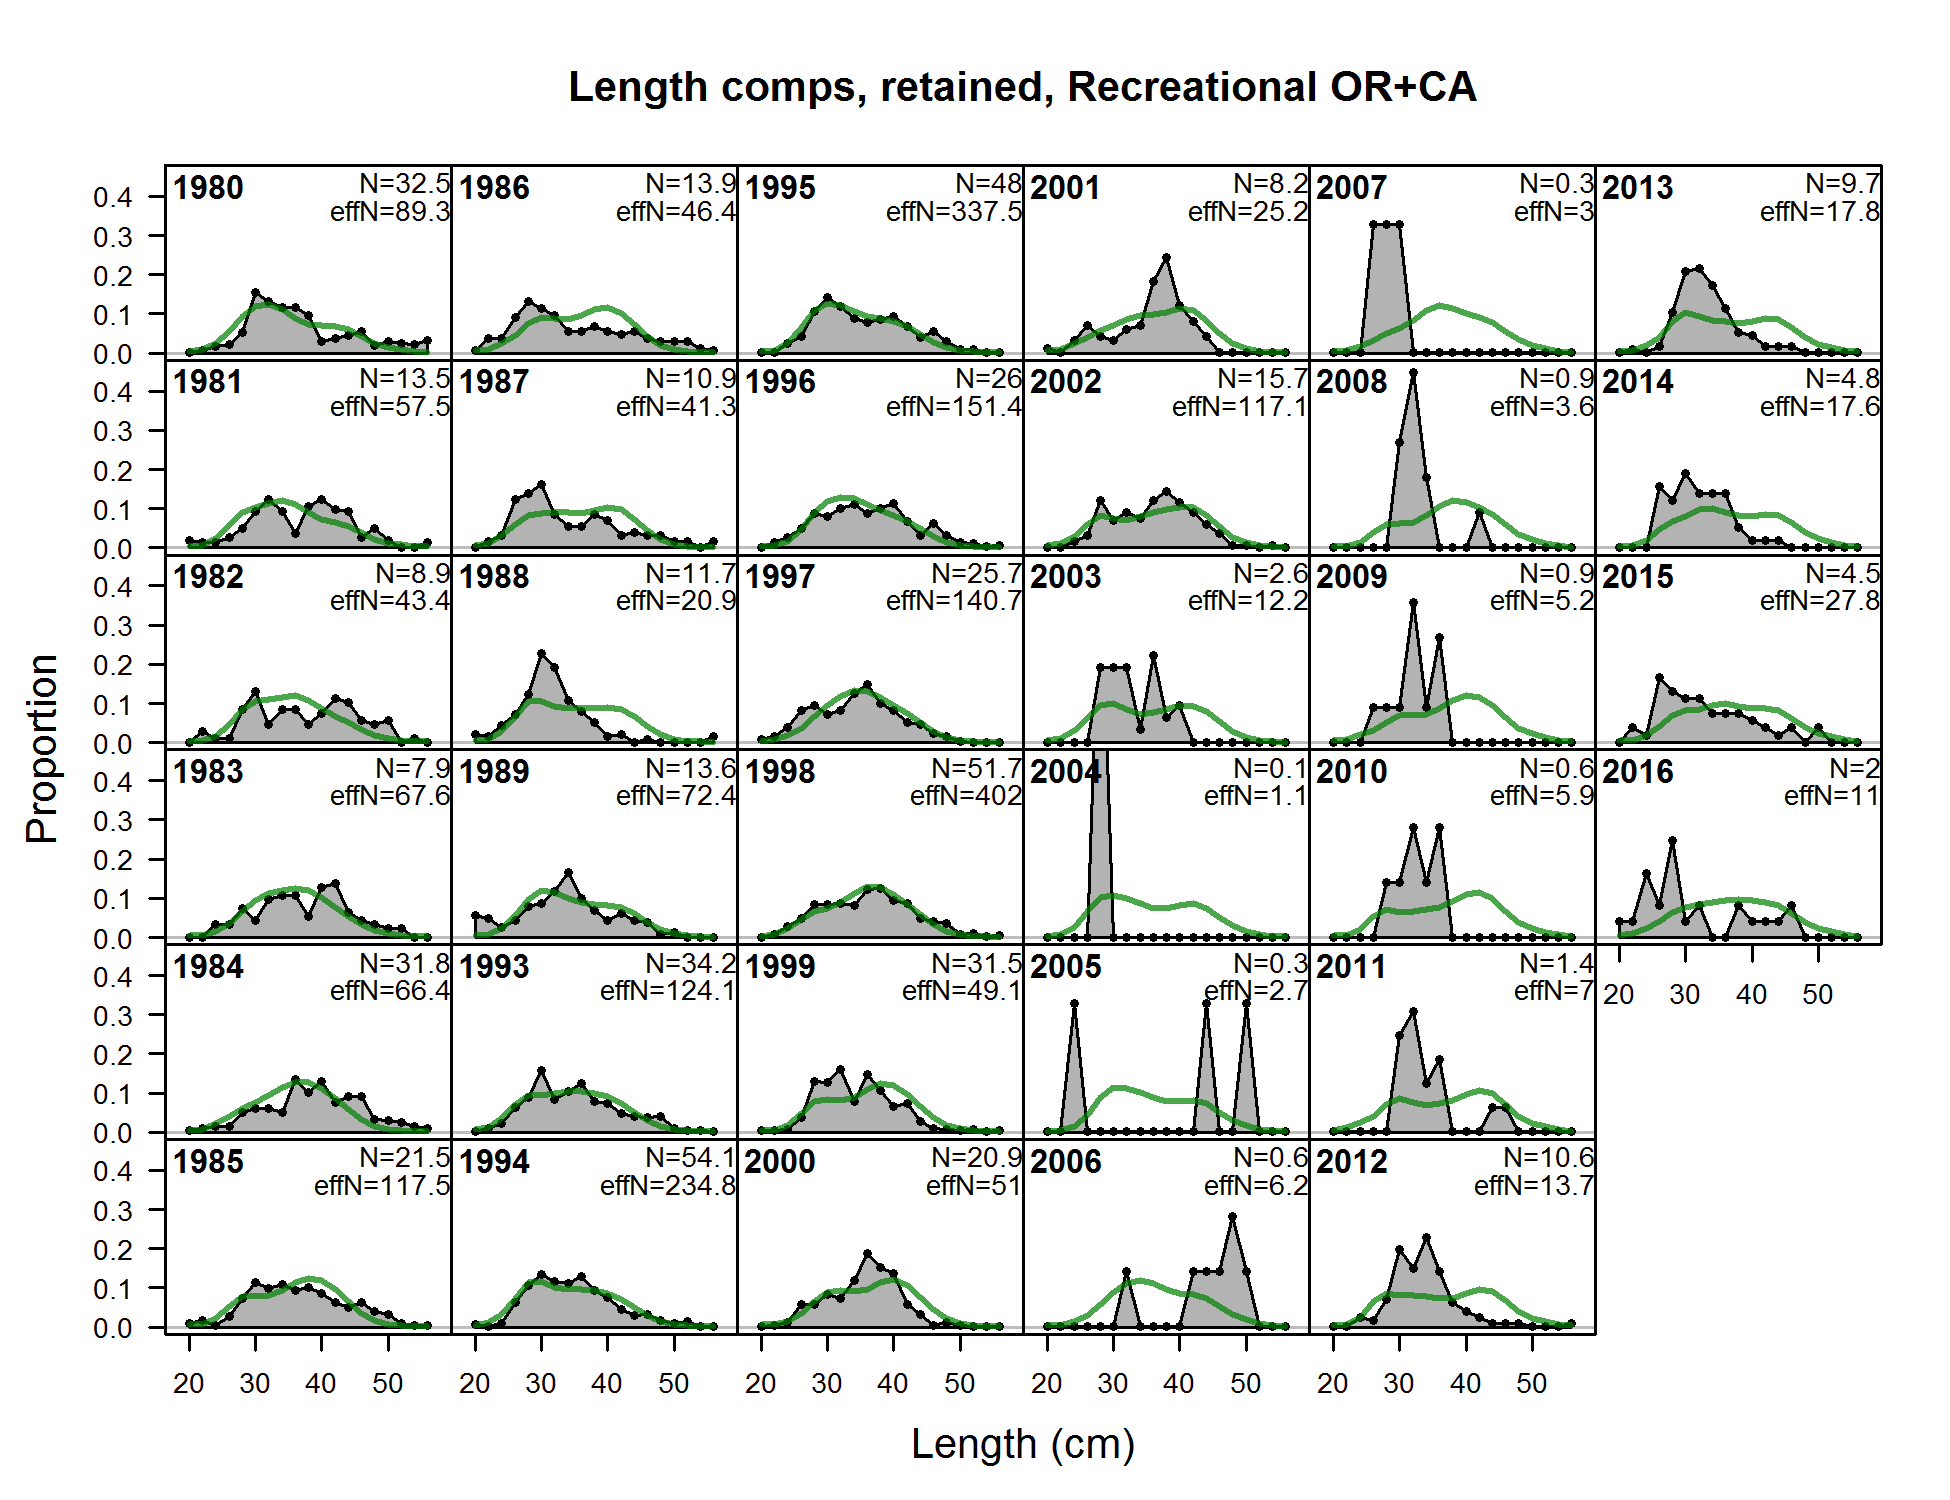
\includegraphics{./r4ss/plots_mod1/comp_lenfit_flt3mkt2.png}
\caption{\textbf{Northern model} Length comps, retained, Recreational
OR+CA \label{fig:mod1_14_comp_lenfit_flt3mkt2}}
\end{figure}

\begin{figure}[htbp]
\centering
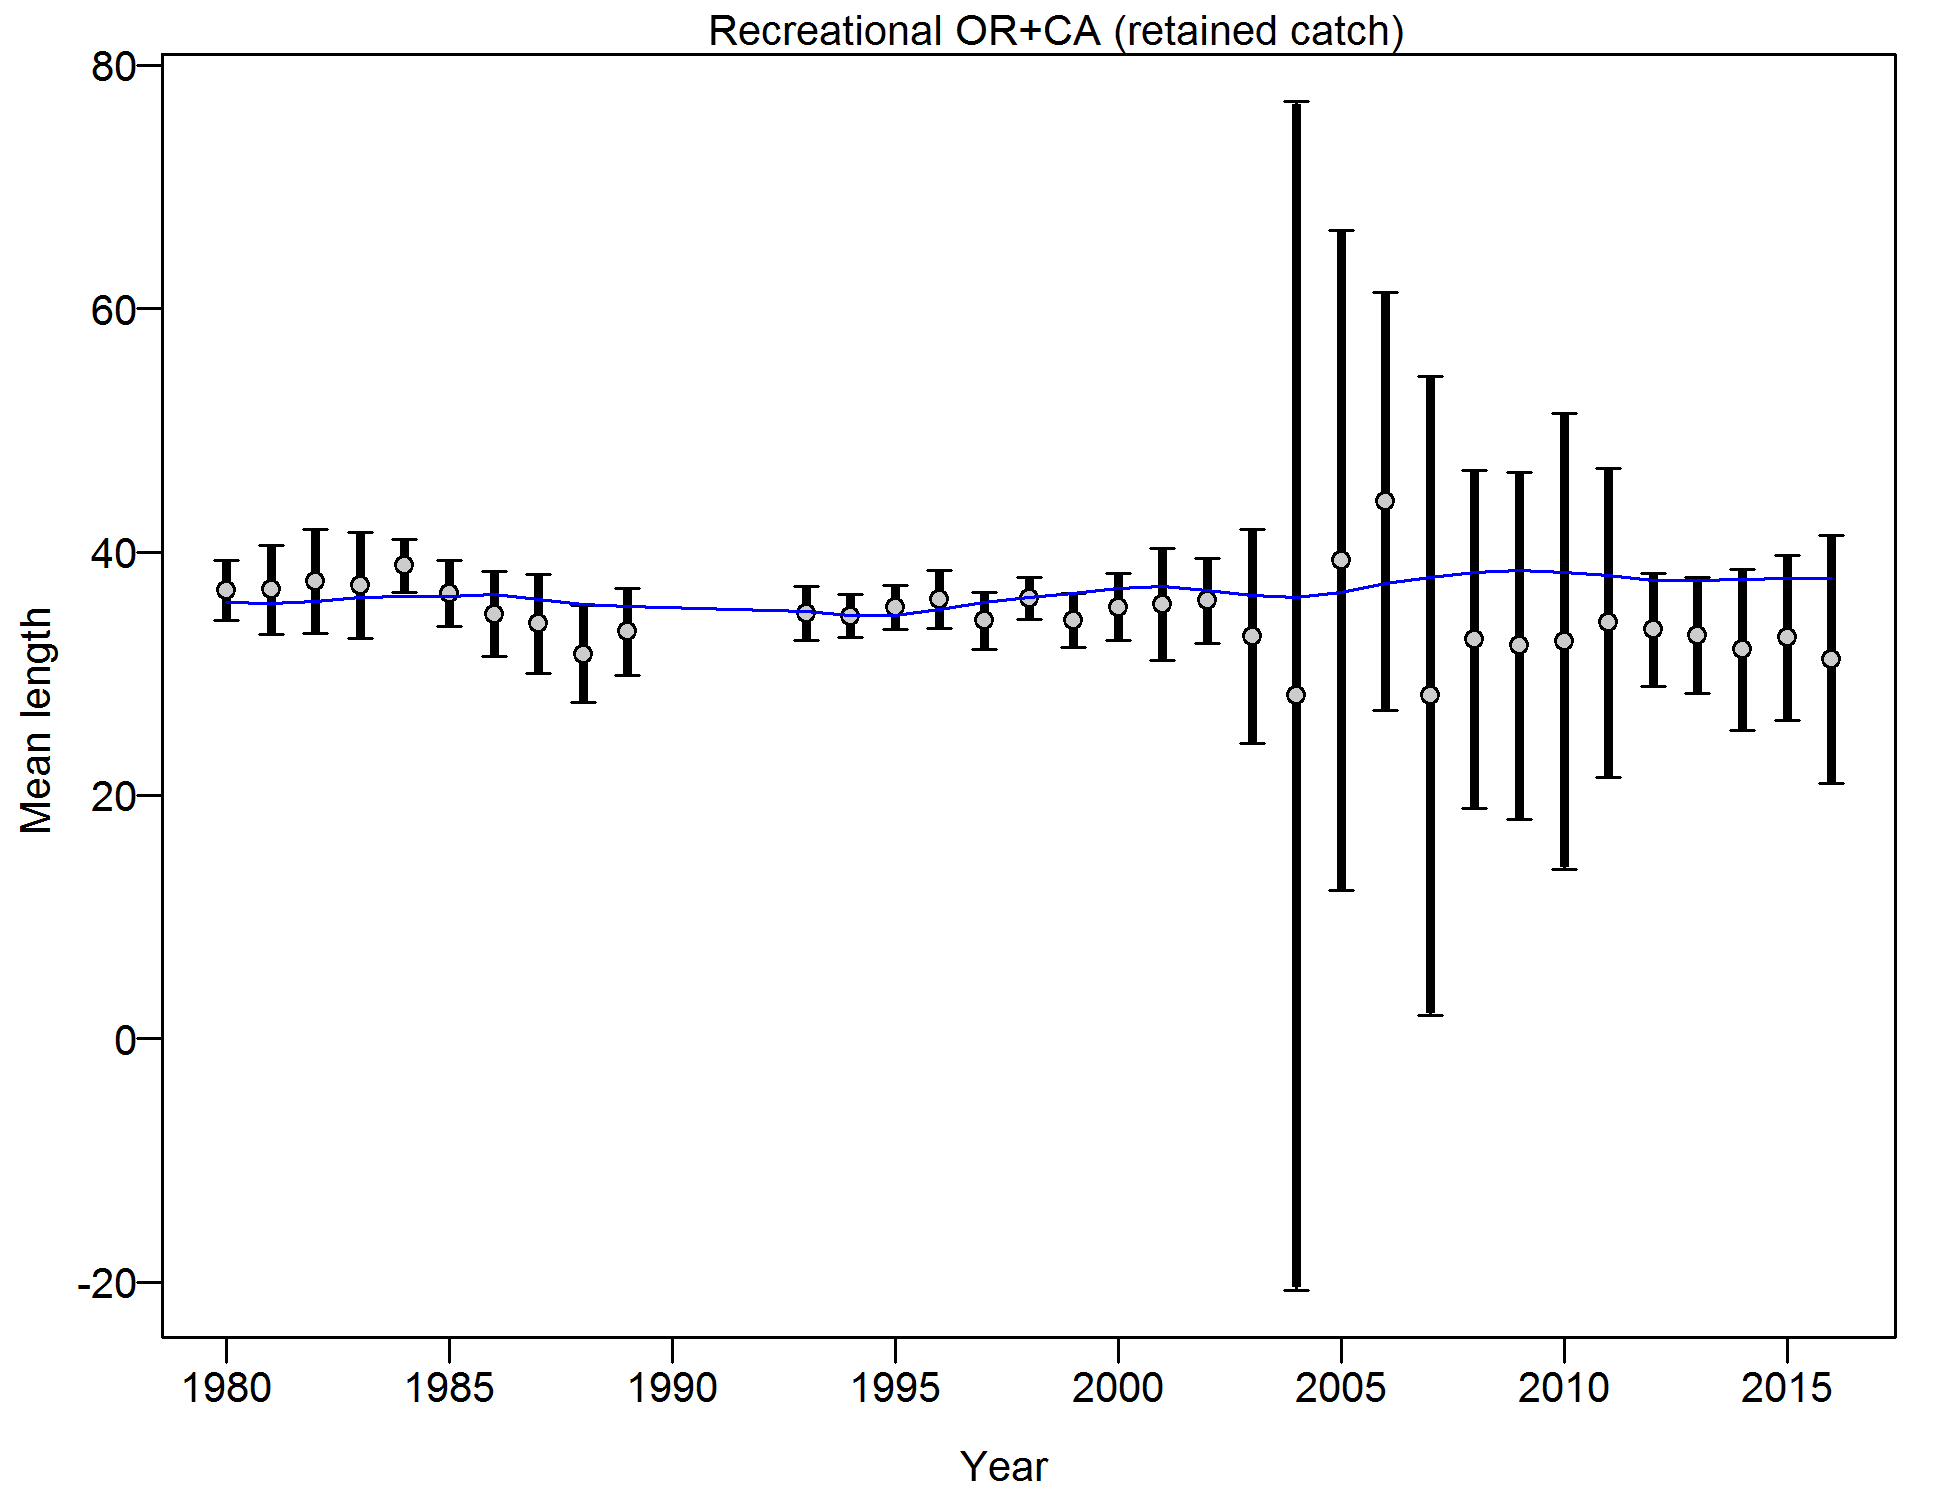
\includegraphics{./r4ss/plots_mod1/comp_lenfit_data_weighting_TA1.8_Recreational OR+CA.png}
\caption{\textbf{Northern model} Mean length for Recreational OR+CA with
95\% confidence intervals based on current samples sizes. Francis data
weighting method TA1.8: thinner intervals (with capped ends) show result
of further adjusting sample sizes based on suggested multiplier (with
95\% interval) for len data from Recreational OR+CA: 0.9909
(0.6731\_1.7073) For more info, see Francis, R.I.C.C. (2011). Data
weighting in statistical fisheries stock assessment models. Can. J.
Fish. Aquat. Sci. 68: 1124\_1138.
\label{fig:mod1_17_comp_lenfit_data_weighting_TA1.8_Recreational OR+CA}}
\end{figure}

\begin{figure}[htbp]
\centering
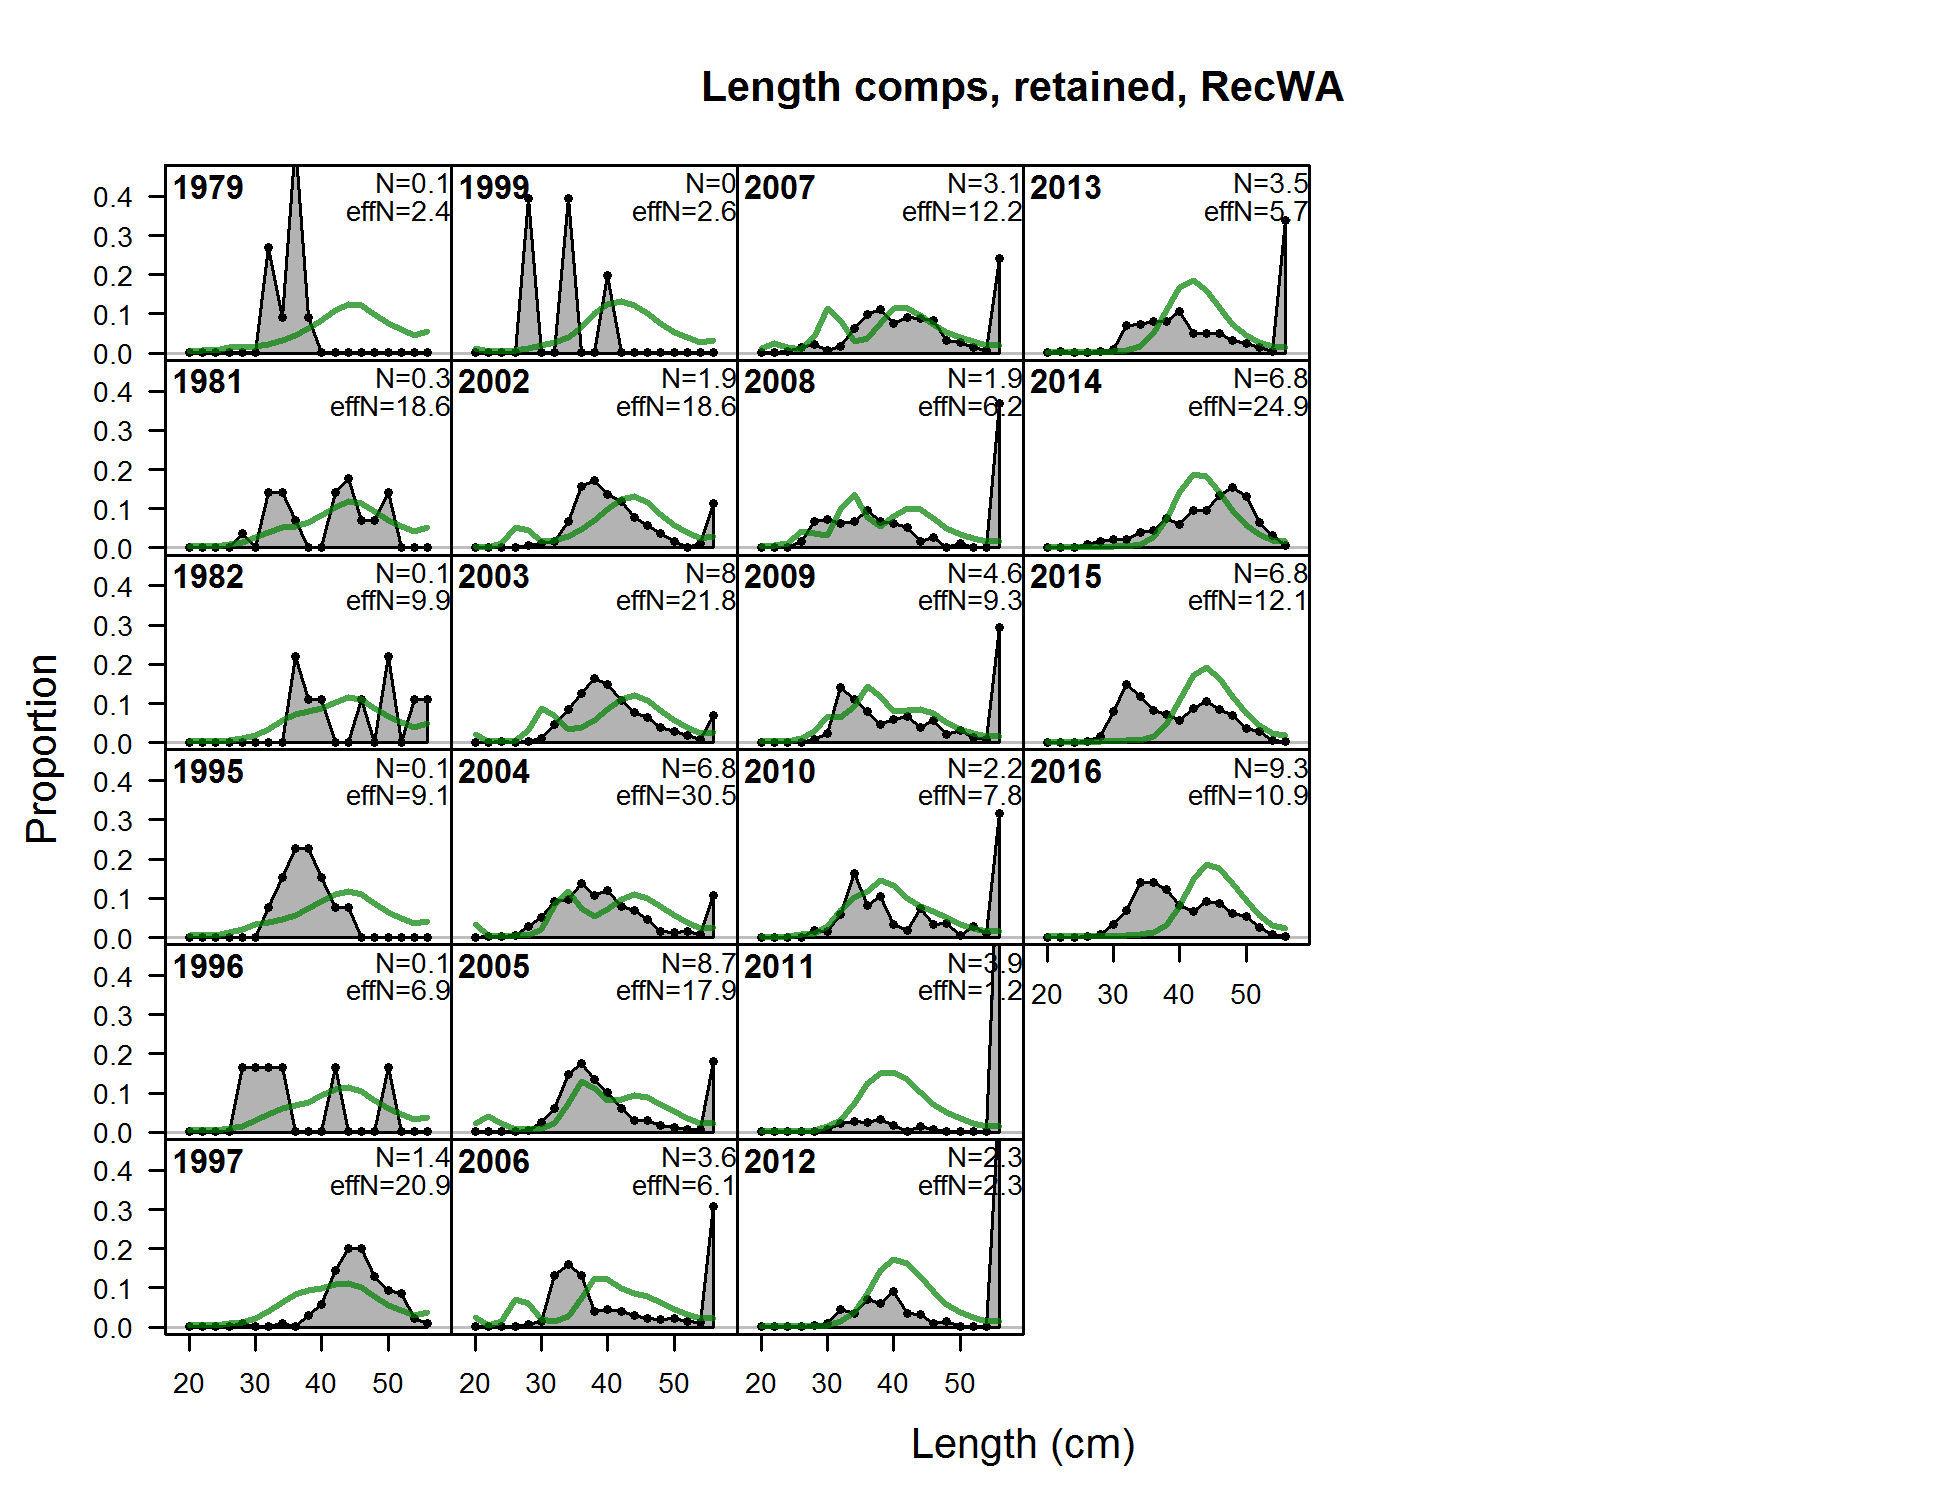
\includegraphics{./r4ss/plots_mod1/comp_lenfit_flt4mkt2.png}
\caption{\textbf{Northern model} Length comps, retained, Recreational WA
\label{fig:mod1_18_comp_lenfit_flt4mkt2}}
\end{figure}

\begin{figure}[htbp]
\centering
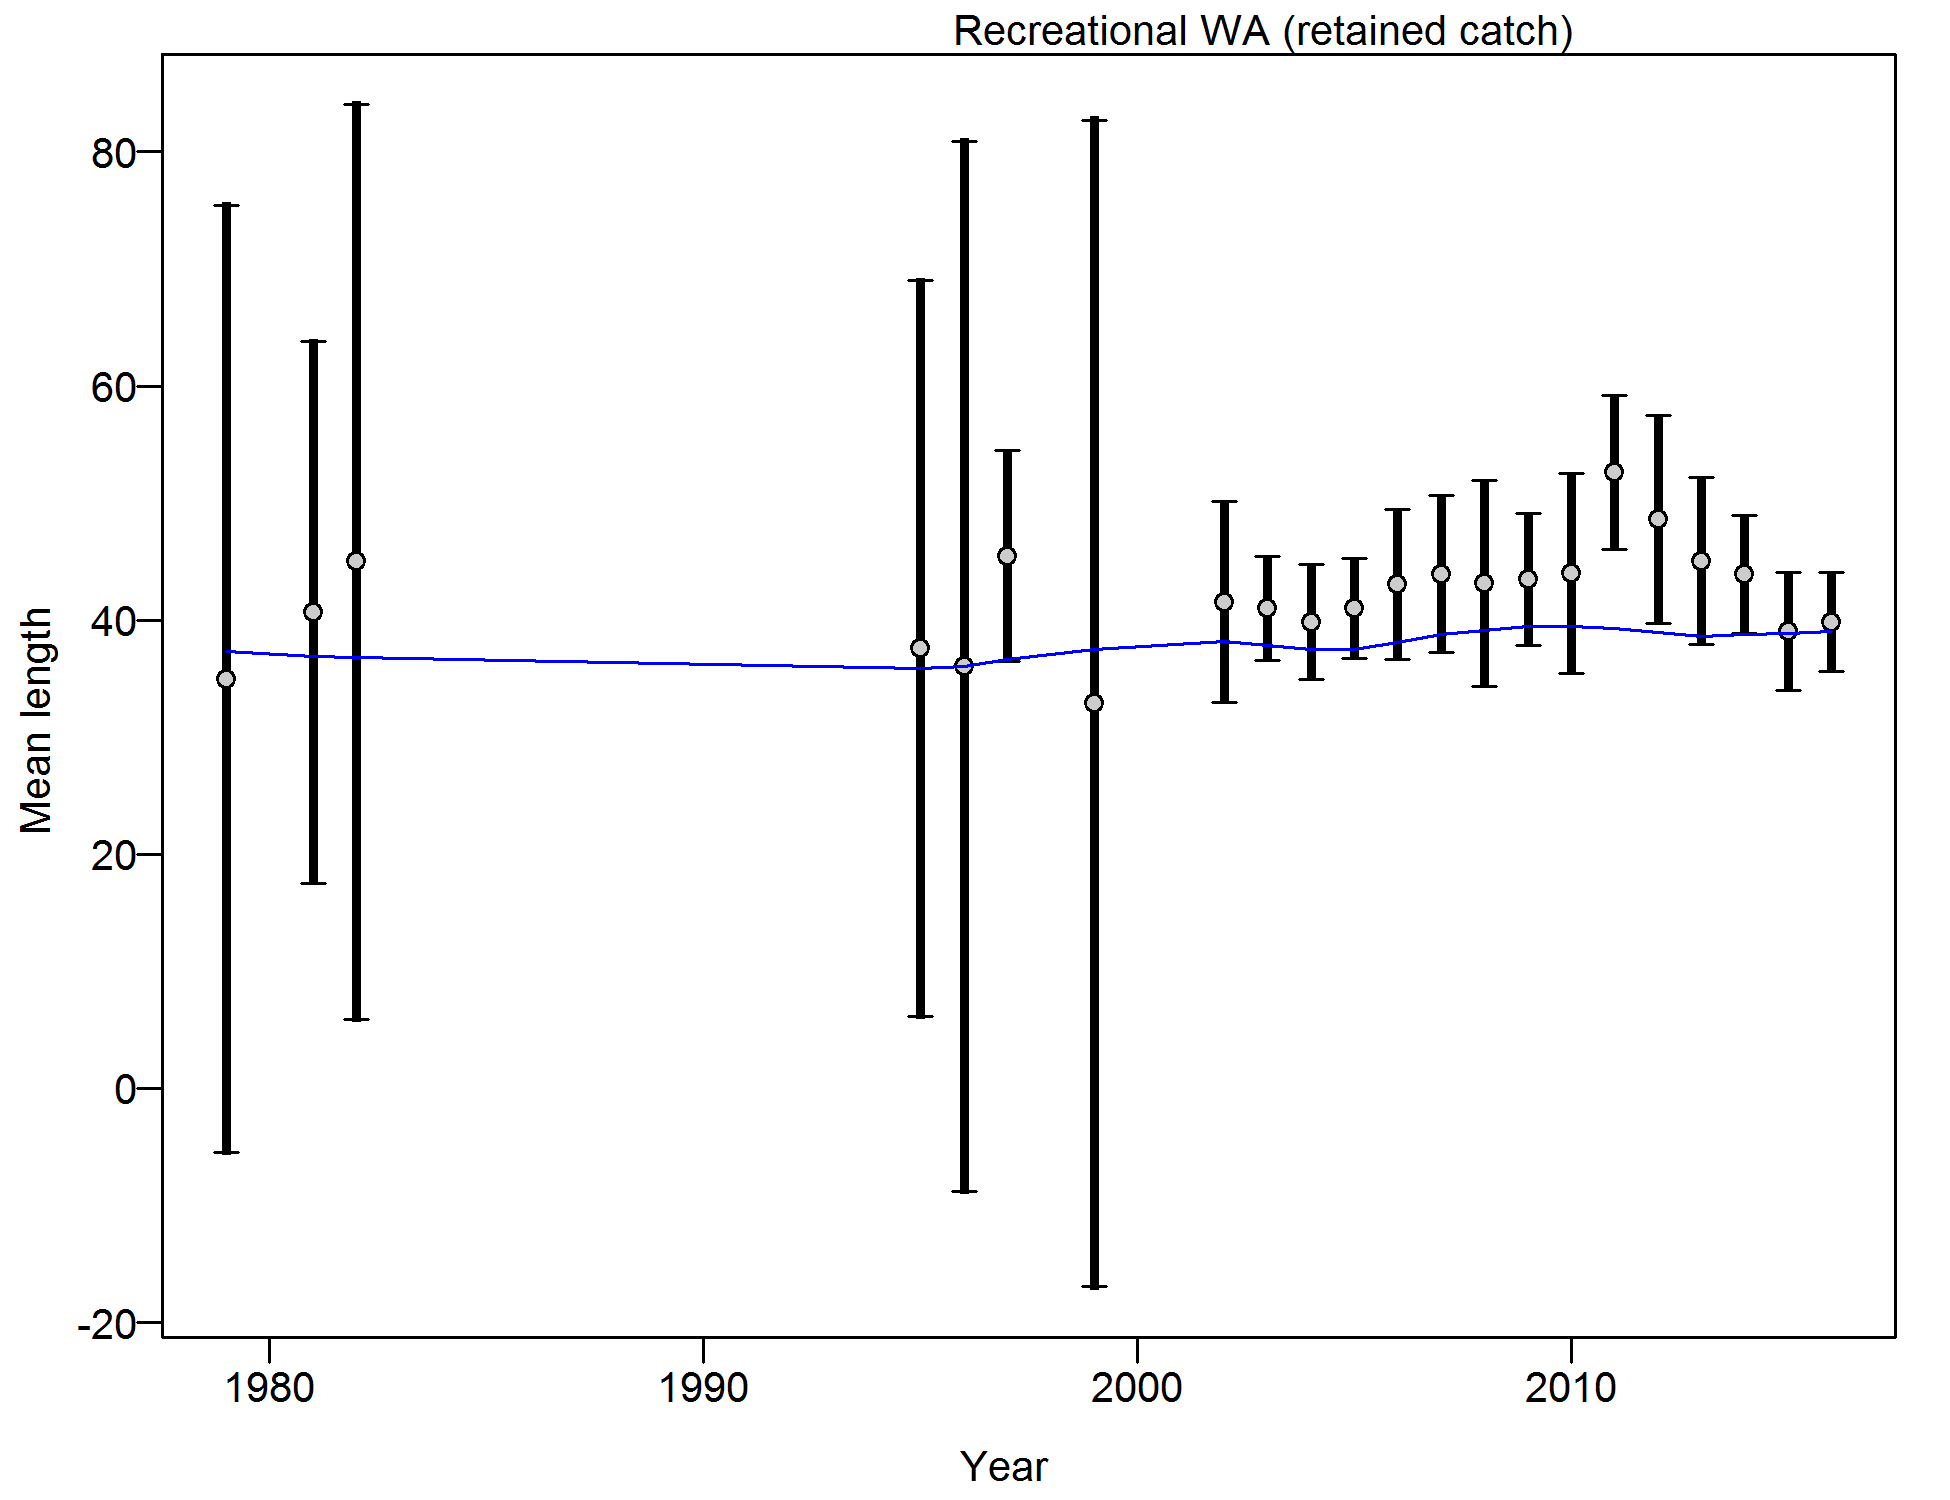
\includegraphics{./r4ss/plots_mod1/comp_lenfit_data_weighting_TA1.8_Recreational WA.png}
\caption{\textbf{Northern model} Mean length for Recreational WA with
95\% confidence intervals based on current samples sizes. Francis data
weighting method TA1.8: thinner intervals (with capped ends) show result
of further adjusting sample sizes based on suggested multiplier (with
95\% interval) for len data from Recreational WA: 1.0056
(0.5535\_2.3815) For more info, see Francis, R.I.C.C. (2011). Data
weighting in statistical fisheries stock assessment models. Can. J.
Fish. Aquat. Sci. 68: 1124\_1138.
\label{fig:mod1_21_comp_lenfit_data_weighting_TA1.8_Recreational WA}}
\end{figure}

\begin{figure}[htbp]
\centering
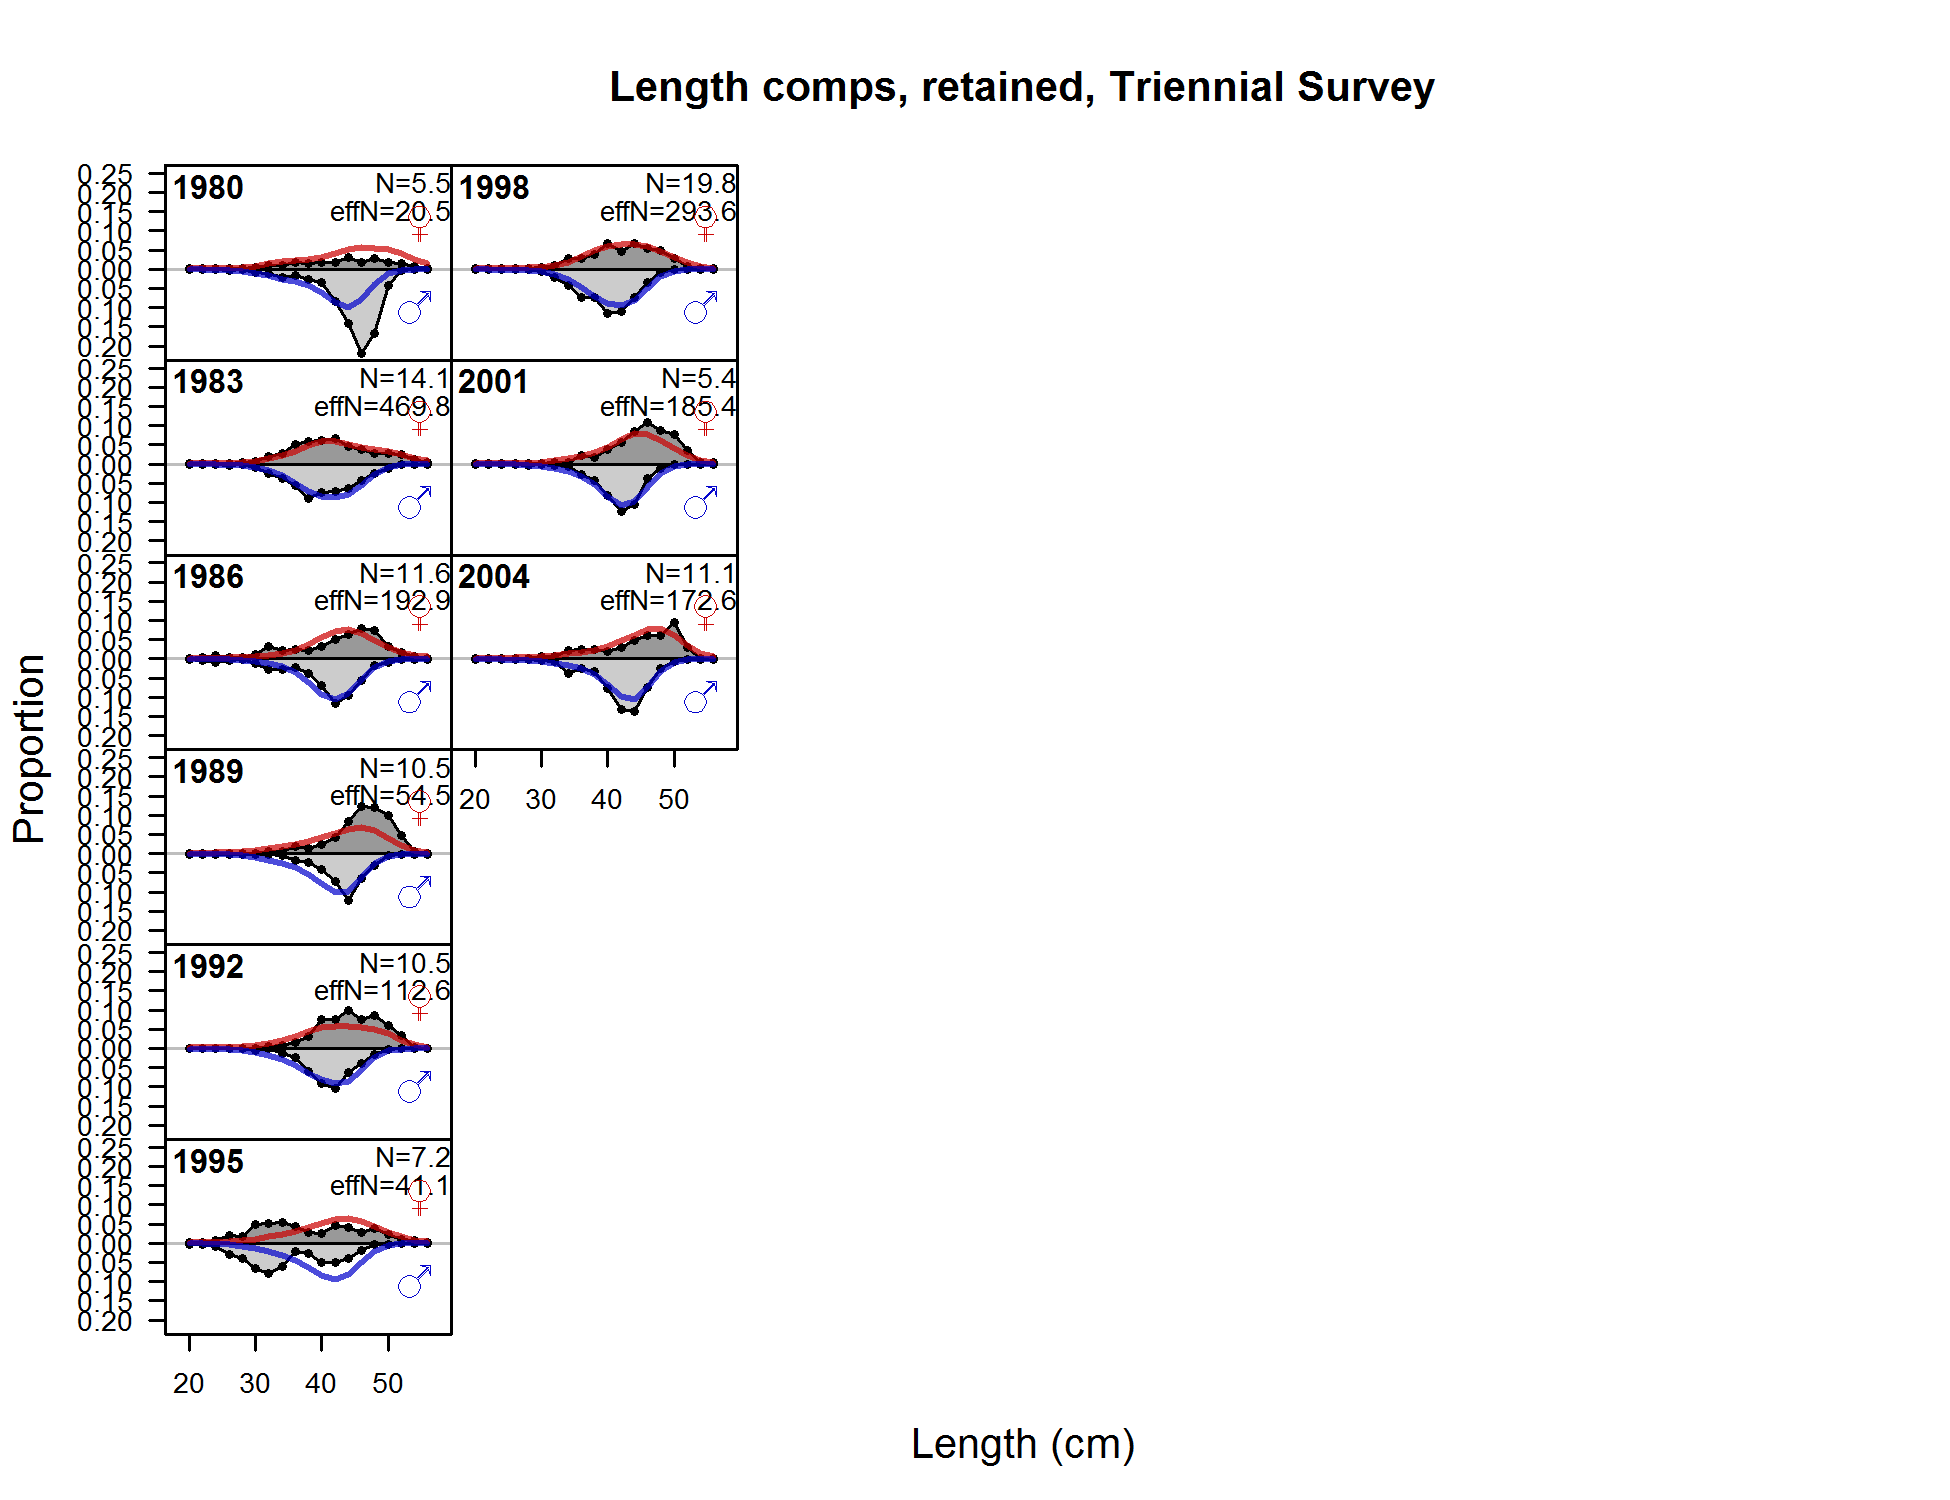
\includegraphics{./r4ss/plots_mod1/comp_lenfit_flt5mkt2.png}
\caption{\textbf{Northern model} Length comps, retained, Triennial
Survey \label{fig:mod1_22_comp_lenfit_flt5mkt2}}
\end{figure}

\begin{figure}[htbp]
\centering
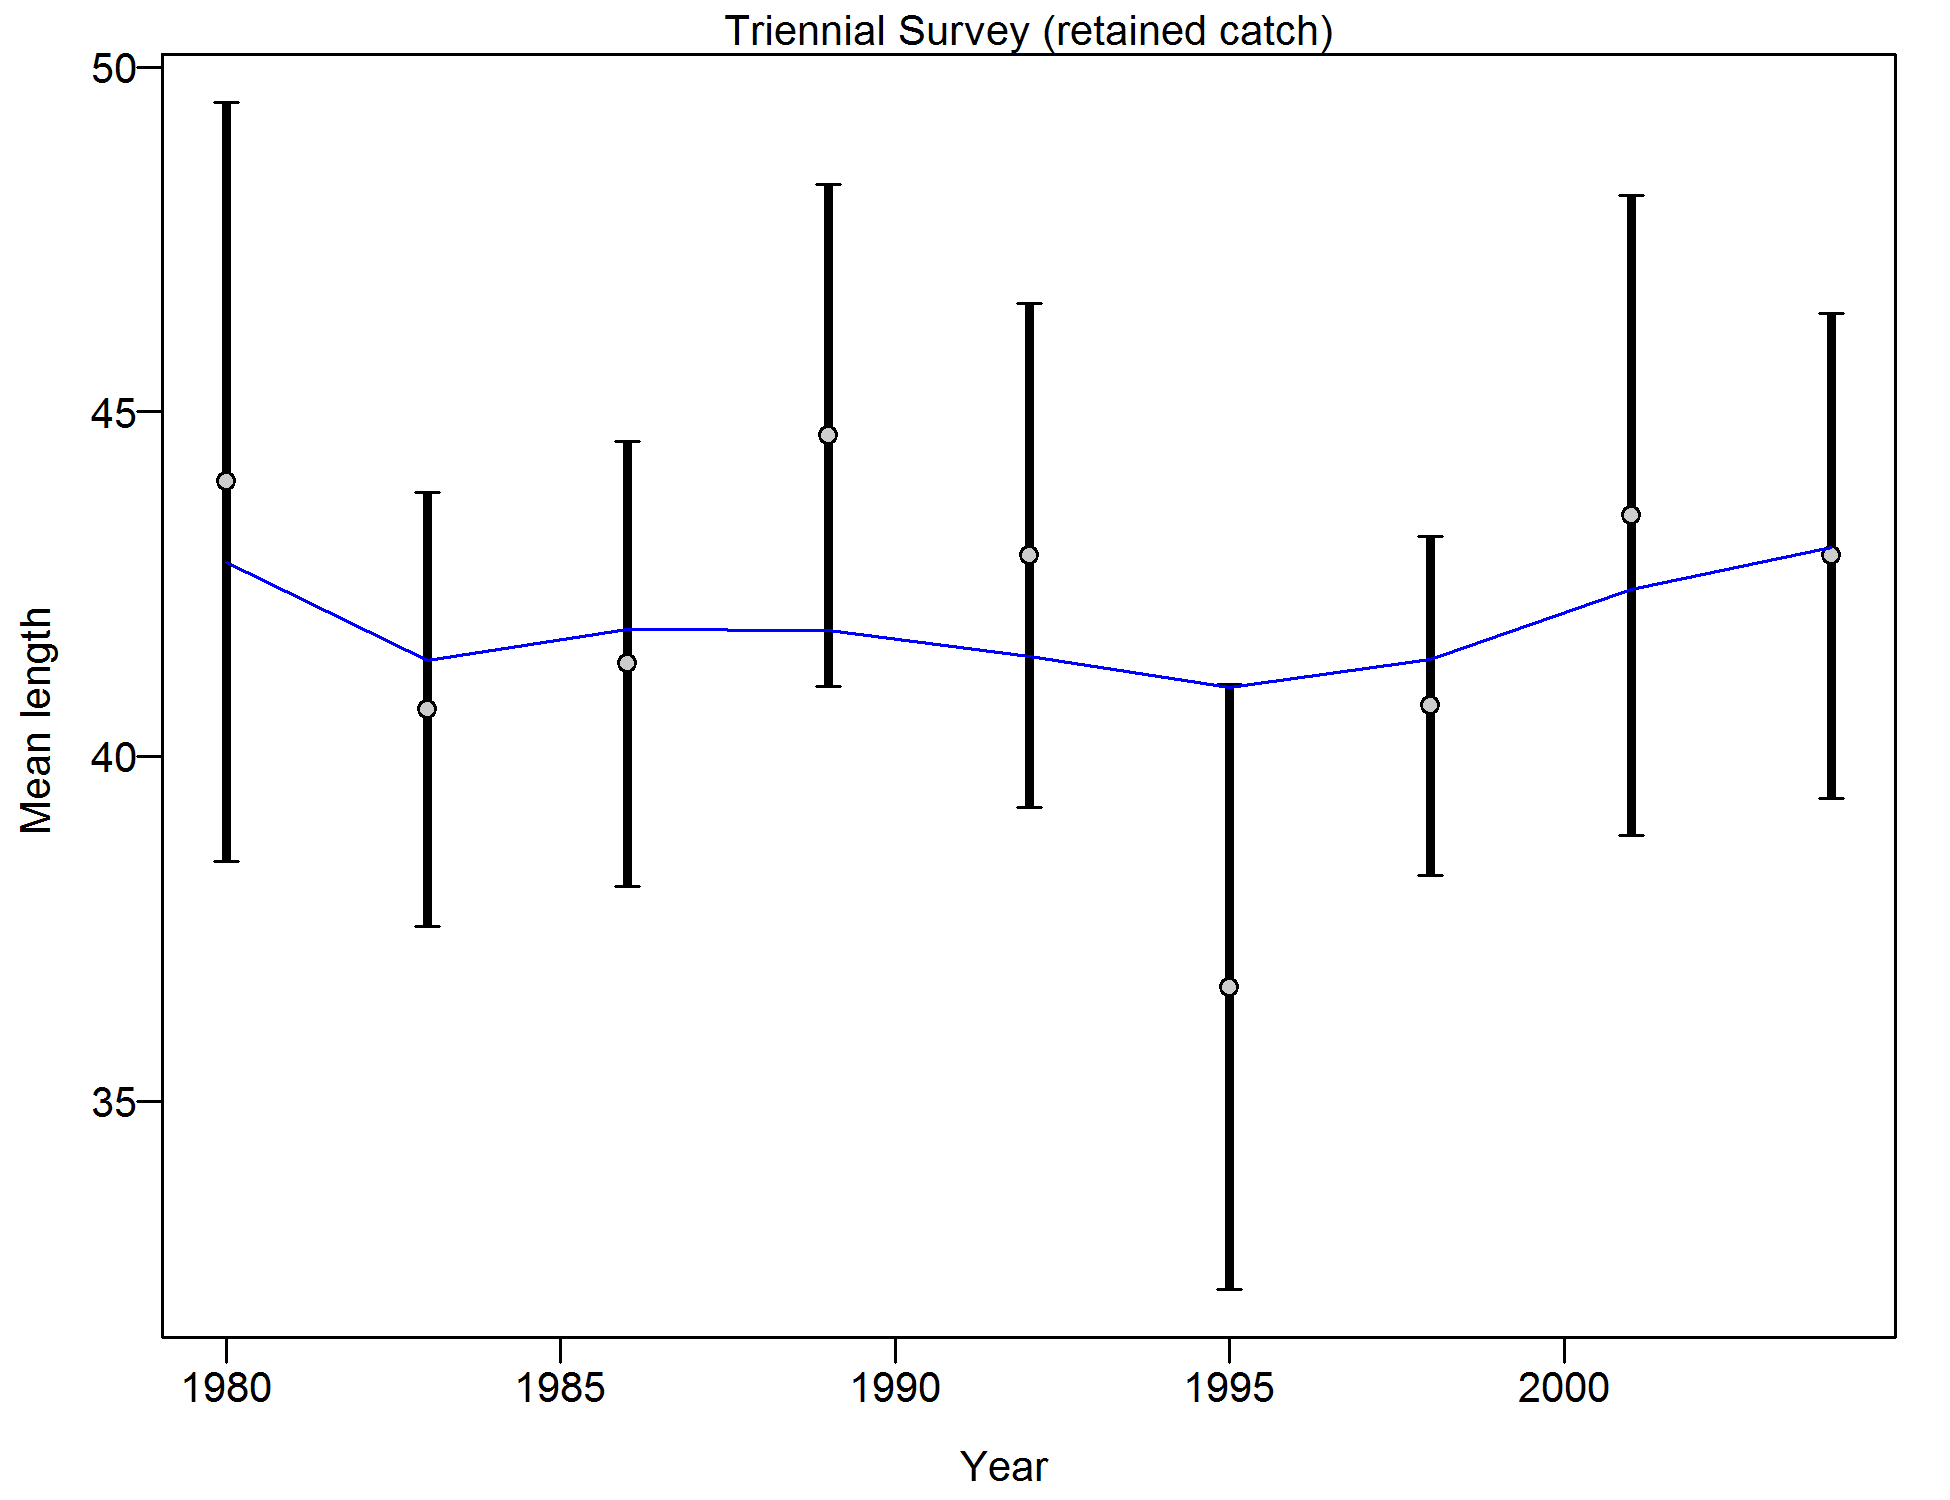
\includegraphics{./r4ss/plots_mod1/comp_lenfit_data_weighting_TA1.8_Triennial Survey.png}
\caption{\textbf{Northern model} Mean length for Triennial Survey with
95\% confidence intervals based on current samples sizes. Francis data
weighting method TA1.8: thinner intervals (with capped ends) show result
of further adjusting sample sizes based on suggested multiplier (with
95\% interval) for len data from Triennial Survey: 0.9901
(0.5251\_5.0869) For more info, see Francis, R.I.C.C. (2011). Data
weighting in statistical fisheries stock assessment models. Can. J.
Fish. Aquat. Sci. 68: 1124\_1138.
\label{fig:mod1_25_comp_lenfit_data_weighting_TA1.8_Triennial Survey}}
\end{figure}

\begin{figure}[htbp]
\centering
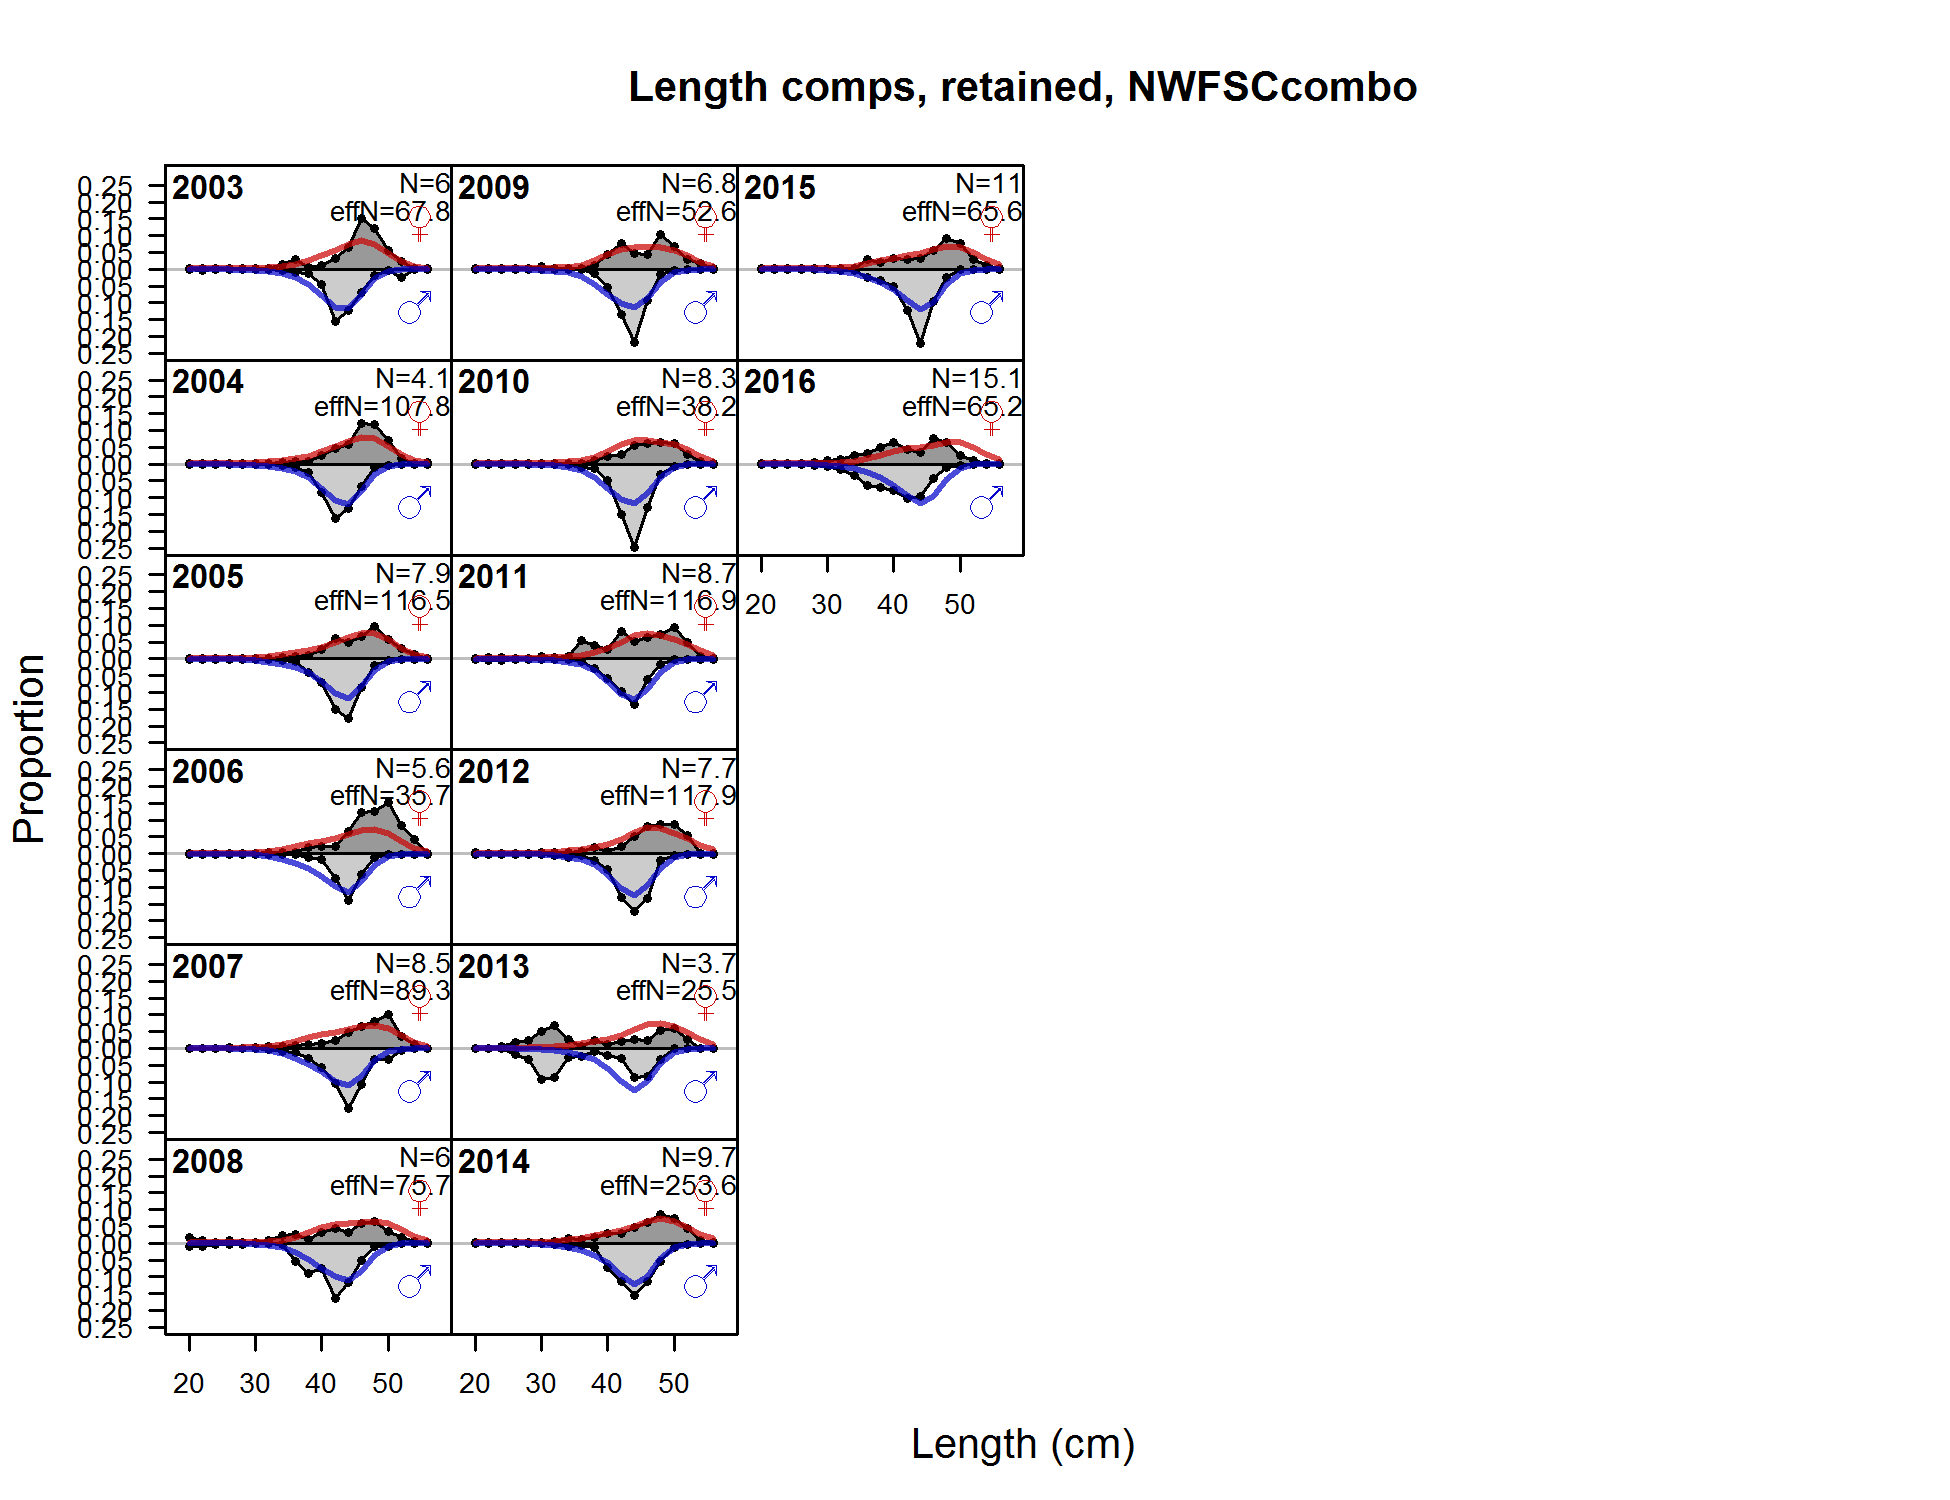
\includegraphics{./r4ss/plots_mod1/comp_lenfit_flt6mkt2.png}
\caption{\textbf{Northern model} Length comps, retained, NWFSC Combo
Survey \label{fig:mod1_26_comp_lenfit_flt6mkt2}}
\end{figure}

\begin{figure}[htbp]
\centering
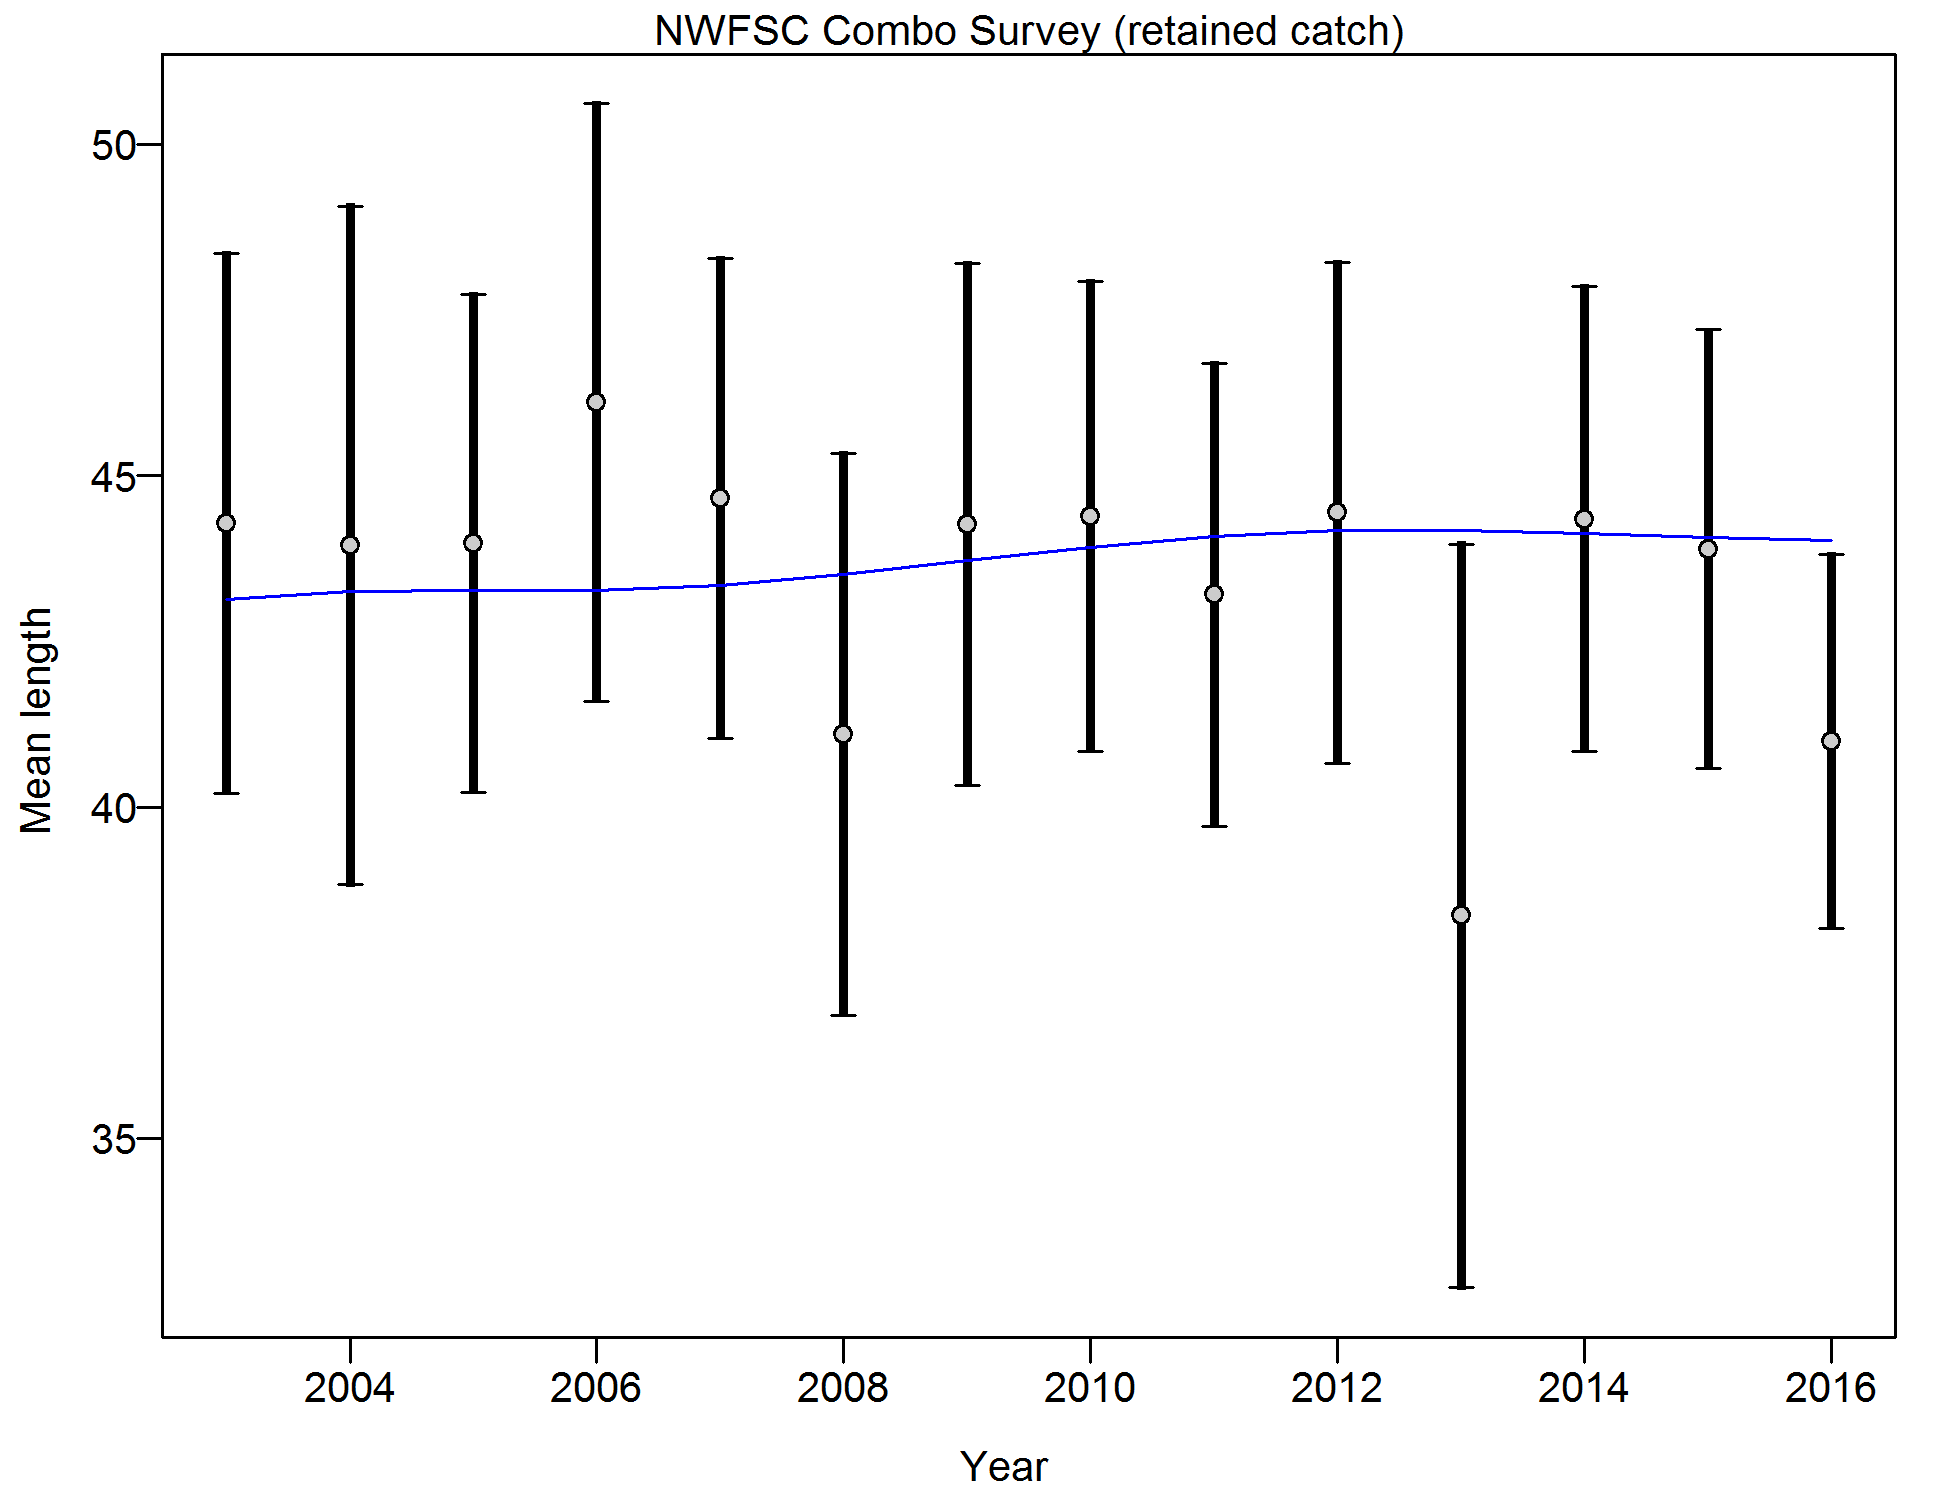
\includegraphics{./r4ss/plots_mod1/comp_lenfit_data_weighting_TA1.8_NWFSC Combo Survey.png}
\caption{\textbf{Northern model} Mean length for NWFSC Combo Survey with
95\% confidence intervals based on current samples sizes. Francis data
weighting method TA1.8: thinner intervals (with capped ends) show result
of further adjusting sample sizes based on suggested multiplier (with
95\% interval) for len data from NWFSC Combo Survey: 1.0058
(0.6094\_4.7808) For more info, see Francis, R.I.C.C. (2011). Data
weighting in statistical fisheries stock assessment models. Can. J.
Fish. Aquat. Sci. 68: 1124\_1138.
\label{fig:mod1_29_comp_lenfit_data_weighting_TA1.8_NWFSC Combo Survey}}
\end{figure}

\begin{figure}[htbp]
\centering
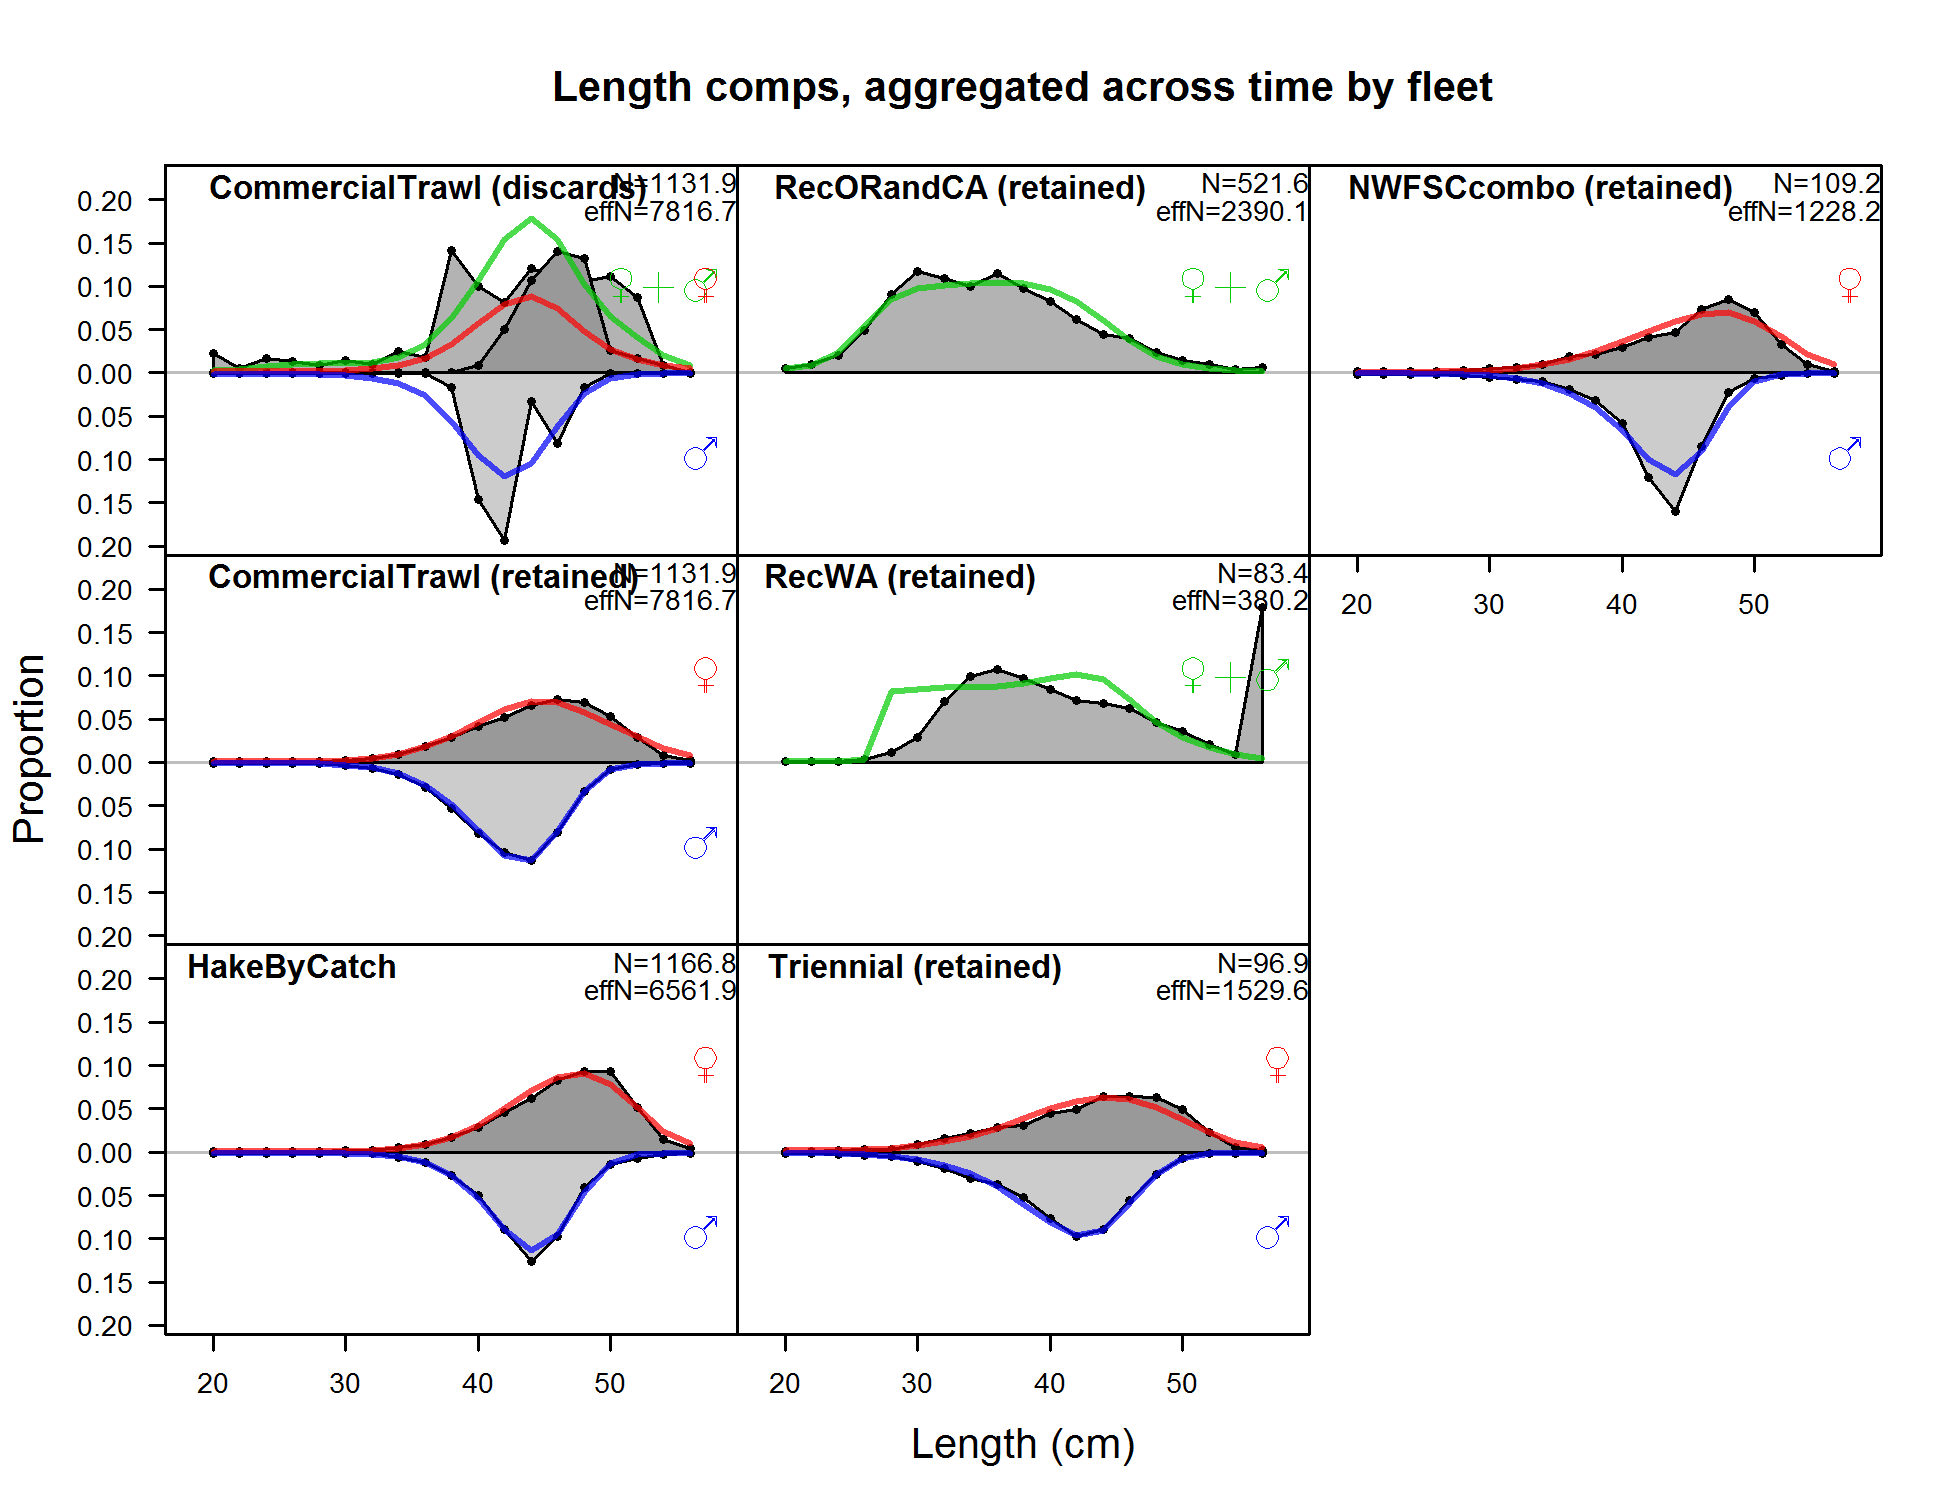
\includegraphics{./r4ss/plots_mod1/comp_lenfit__aggregated_across_time.png}
\caption{\textbf{Northern model} Length comps, aggregated across time by
fleet. Labels `retained' and `discard' indicate discarded or retained
sampled for each fleet. Panels without this designation represent the
whole catch. \label{fig:mod1_30_comp_lenfit__aggregated_across_time}}
\end{figure}

\begin{figure}[htbp]
\centering
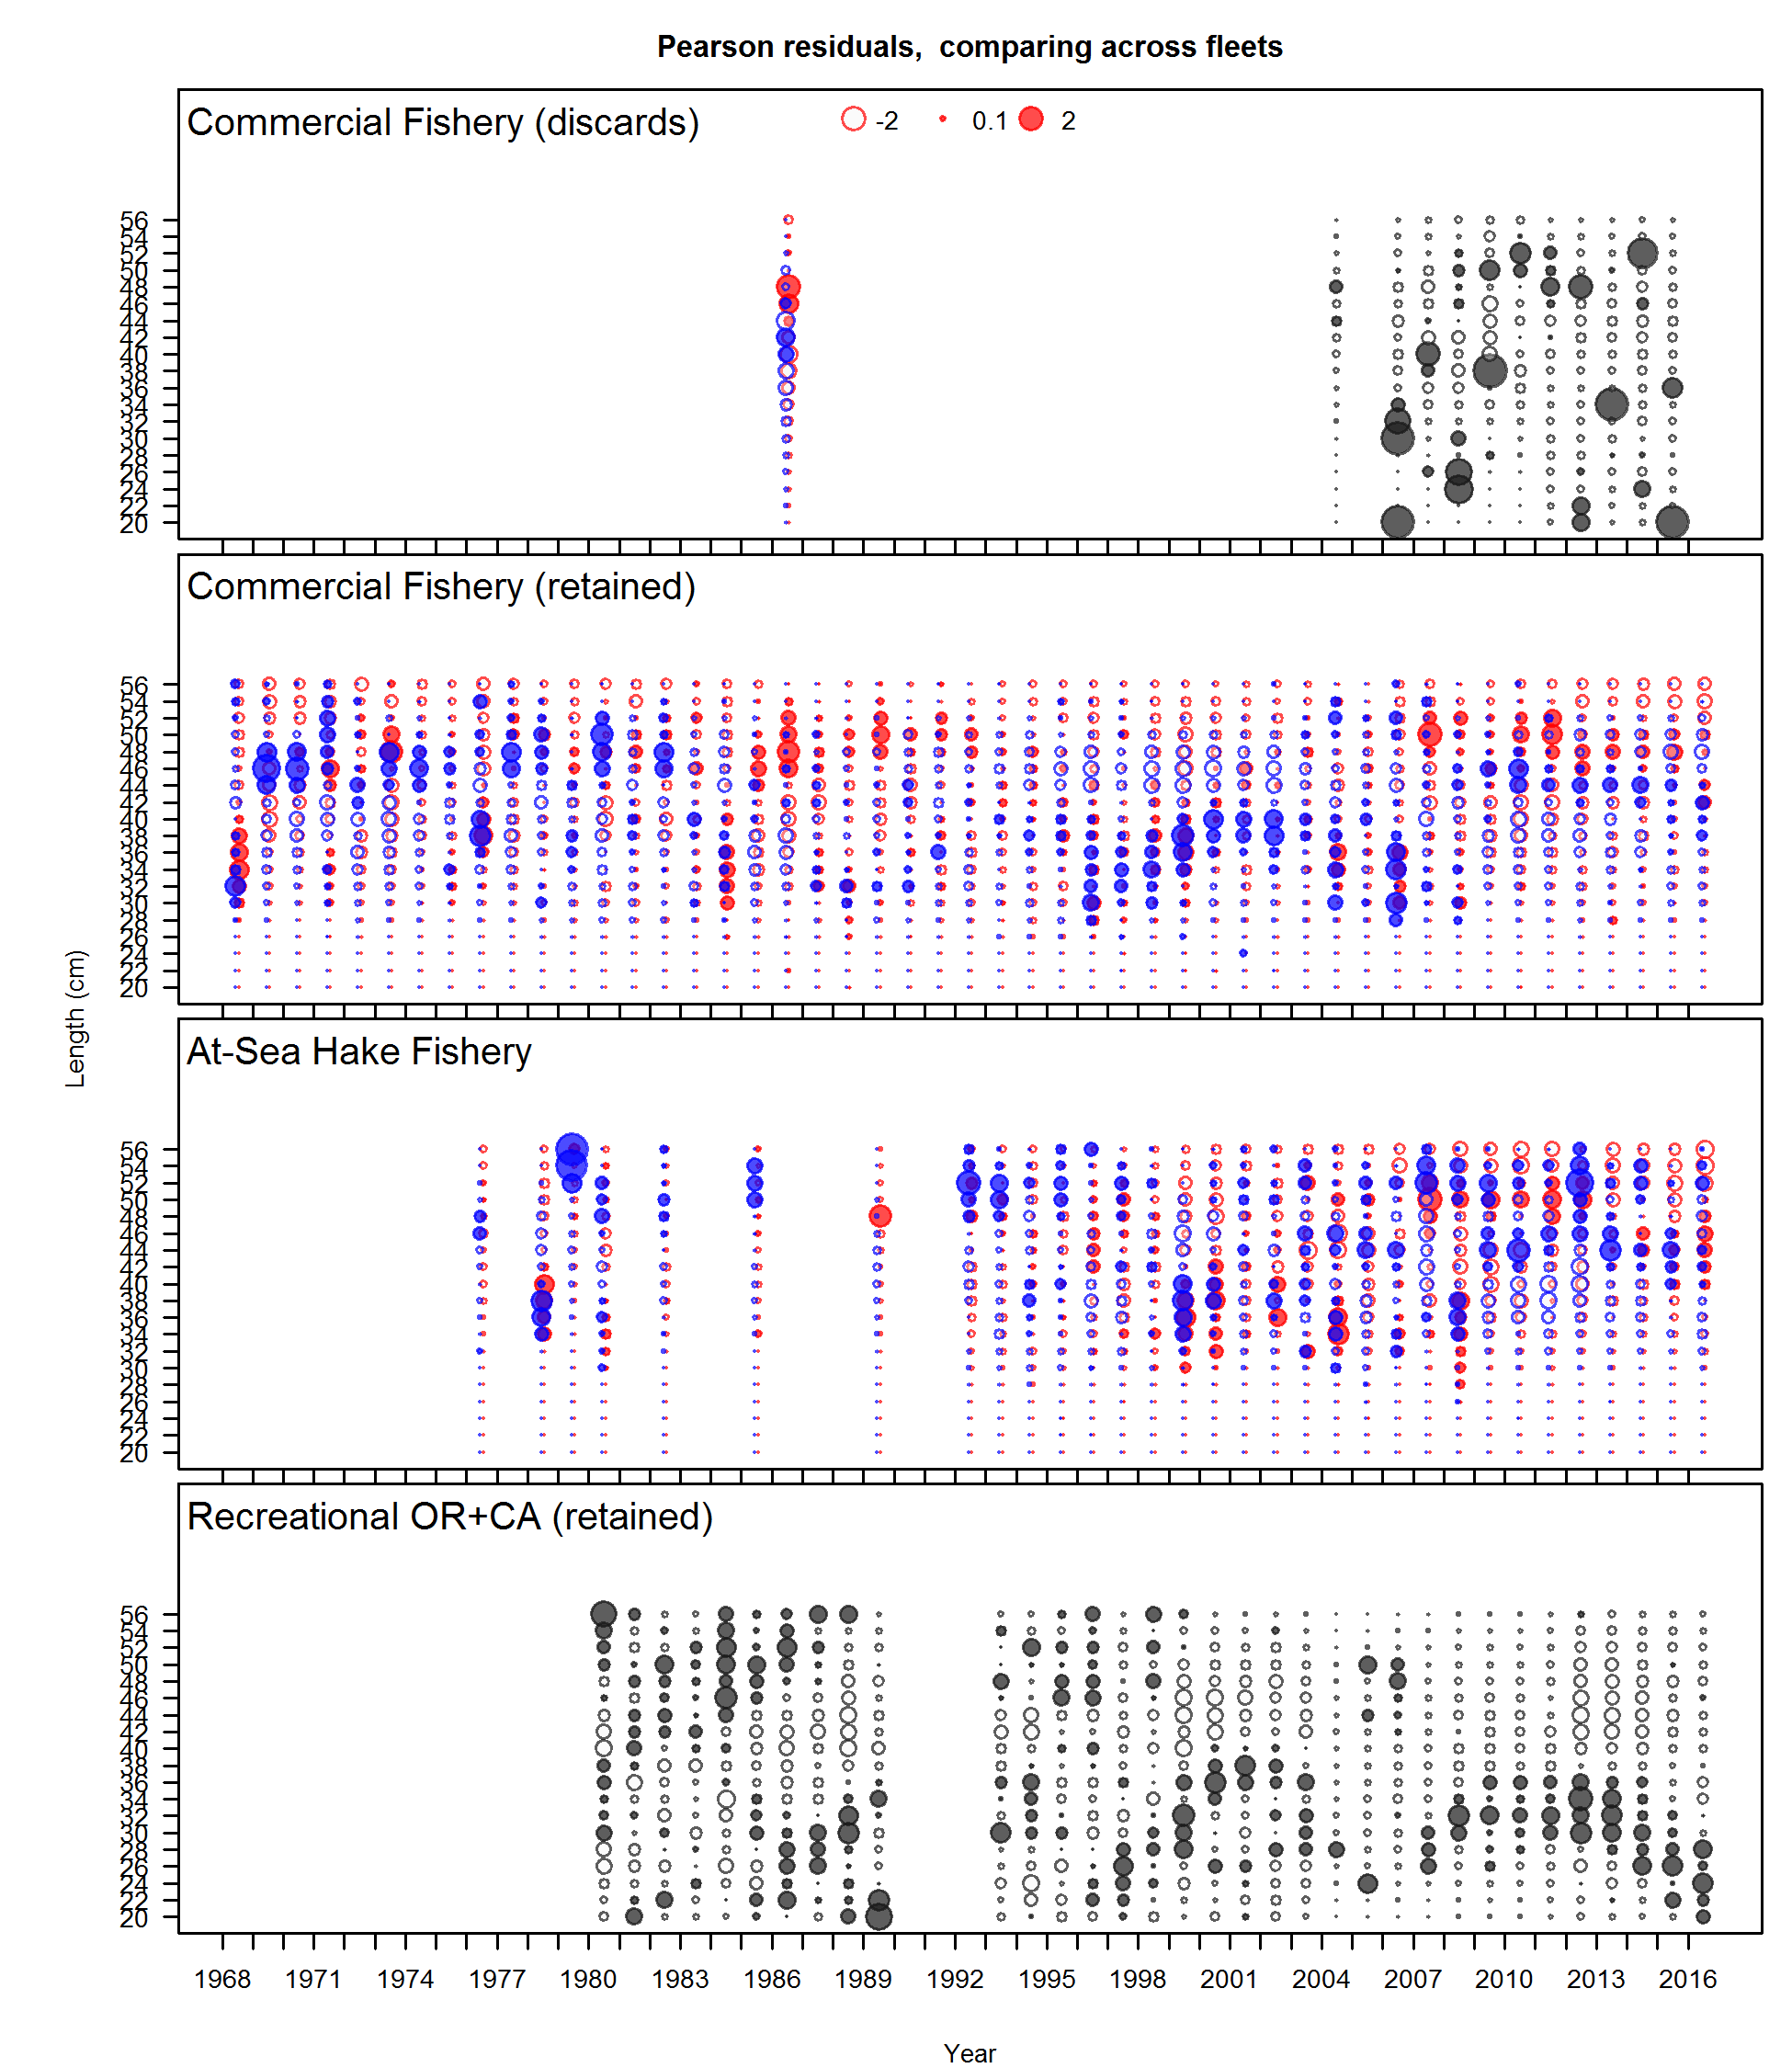
\includegraphics{r4ss/plots_mod1/comp_lenfit__page1_multi-fleet_comparison.png}
\caption{Length composition Pearson residuals for all fleets in the
Northern model (Figure 1 of 2). Closed bubbles are positive residuals
(observed \textgreater{} expected) and open bubbles are negative
residuals (observed \textless{} expected). Bubble colors indicate
unsexed fish (gray), females (red), and males
(blue).\label{fig:comp_Pearson_length_mod1_page1}}
\end{figure}

\begin{figure}[htbp]
\centering
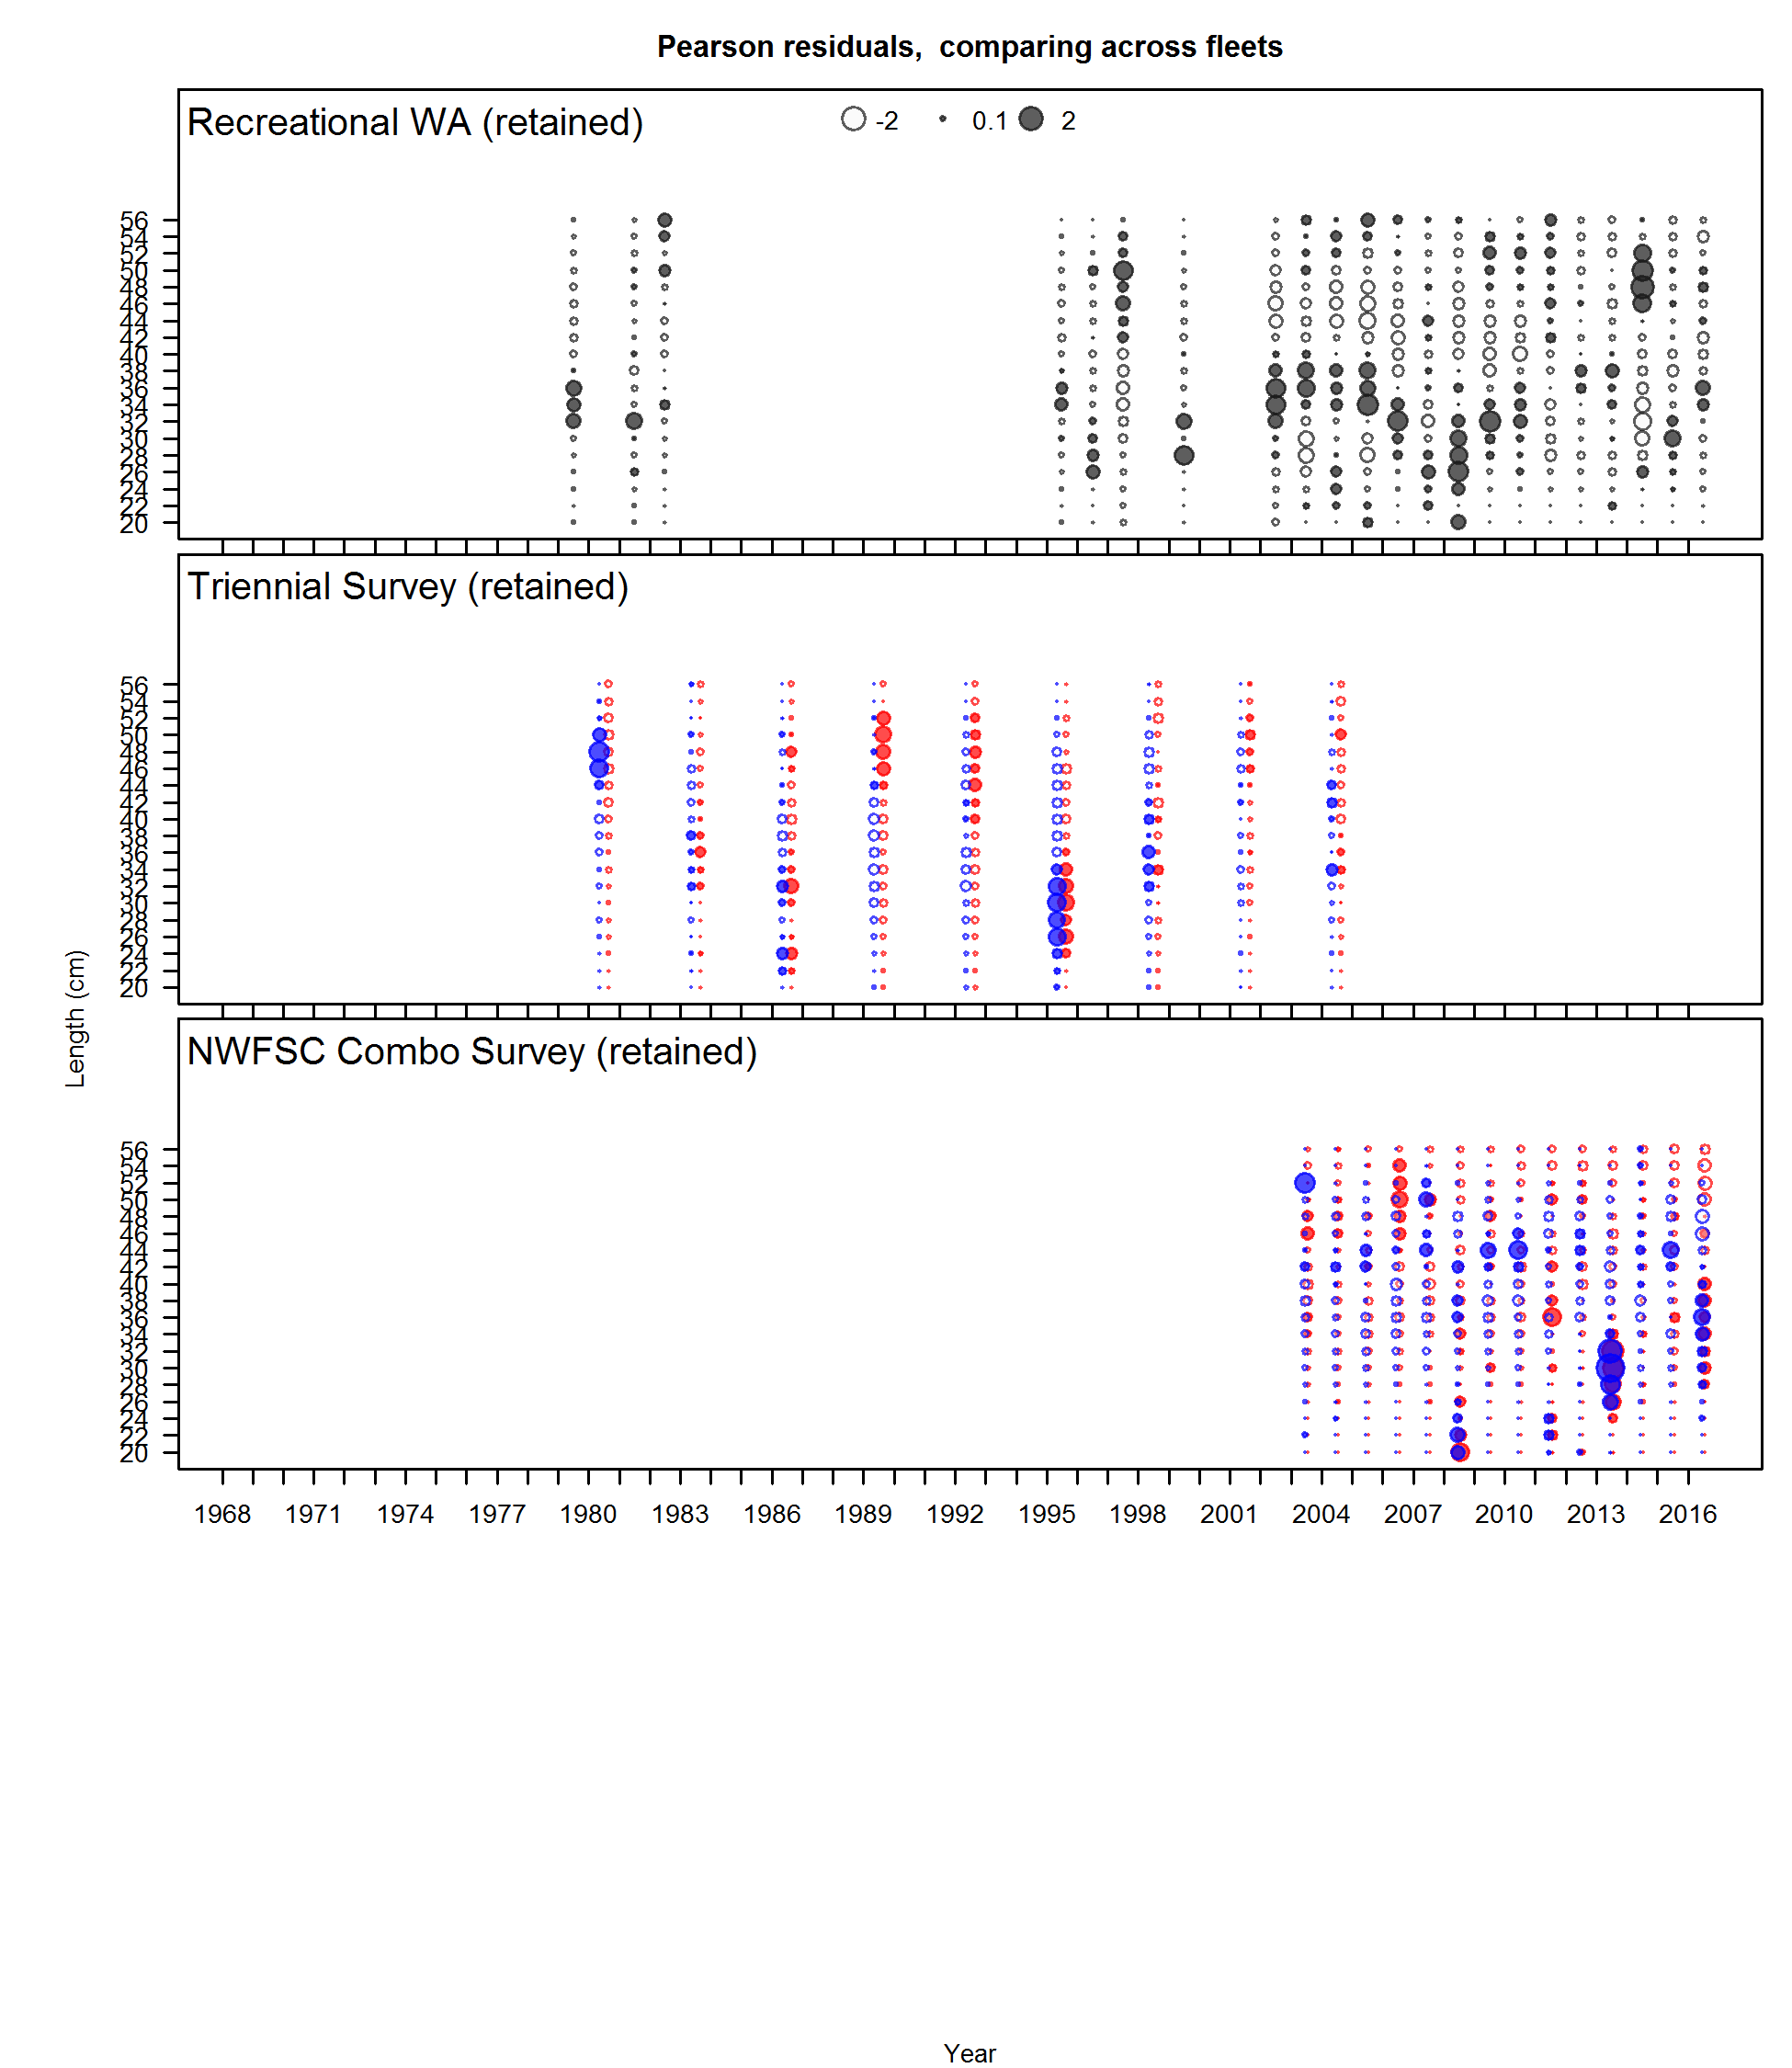
\includegraphics{r4ss/plots_mod1/comp_lenfit__page2_multi-fleet_comparison.png}
\caption{Length composition Pearson residuals for all fleets in the
Northern model (Figure 2 of
2).\label{fig:comp_Pearson_length_mod1_page2}}
\end{figure}

\subsubsection{Fits to age compositions for Northern
model}\label{fits-to-age-compositions-for-northern-model}

\begin{figure}[htbp]
\centering
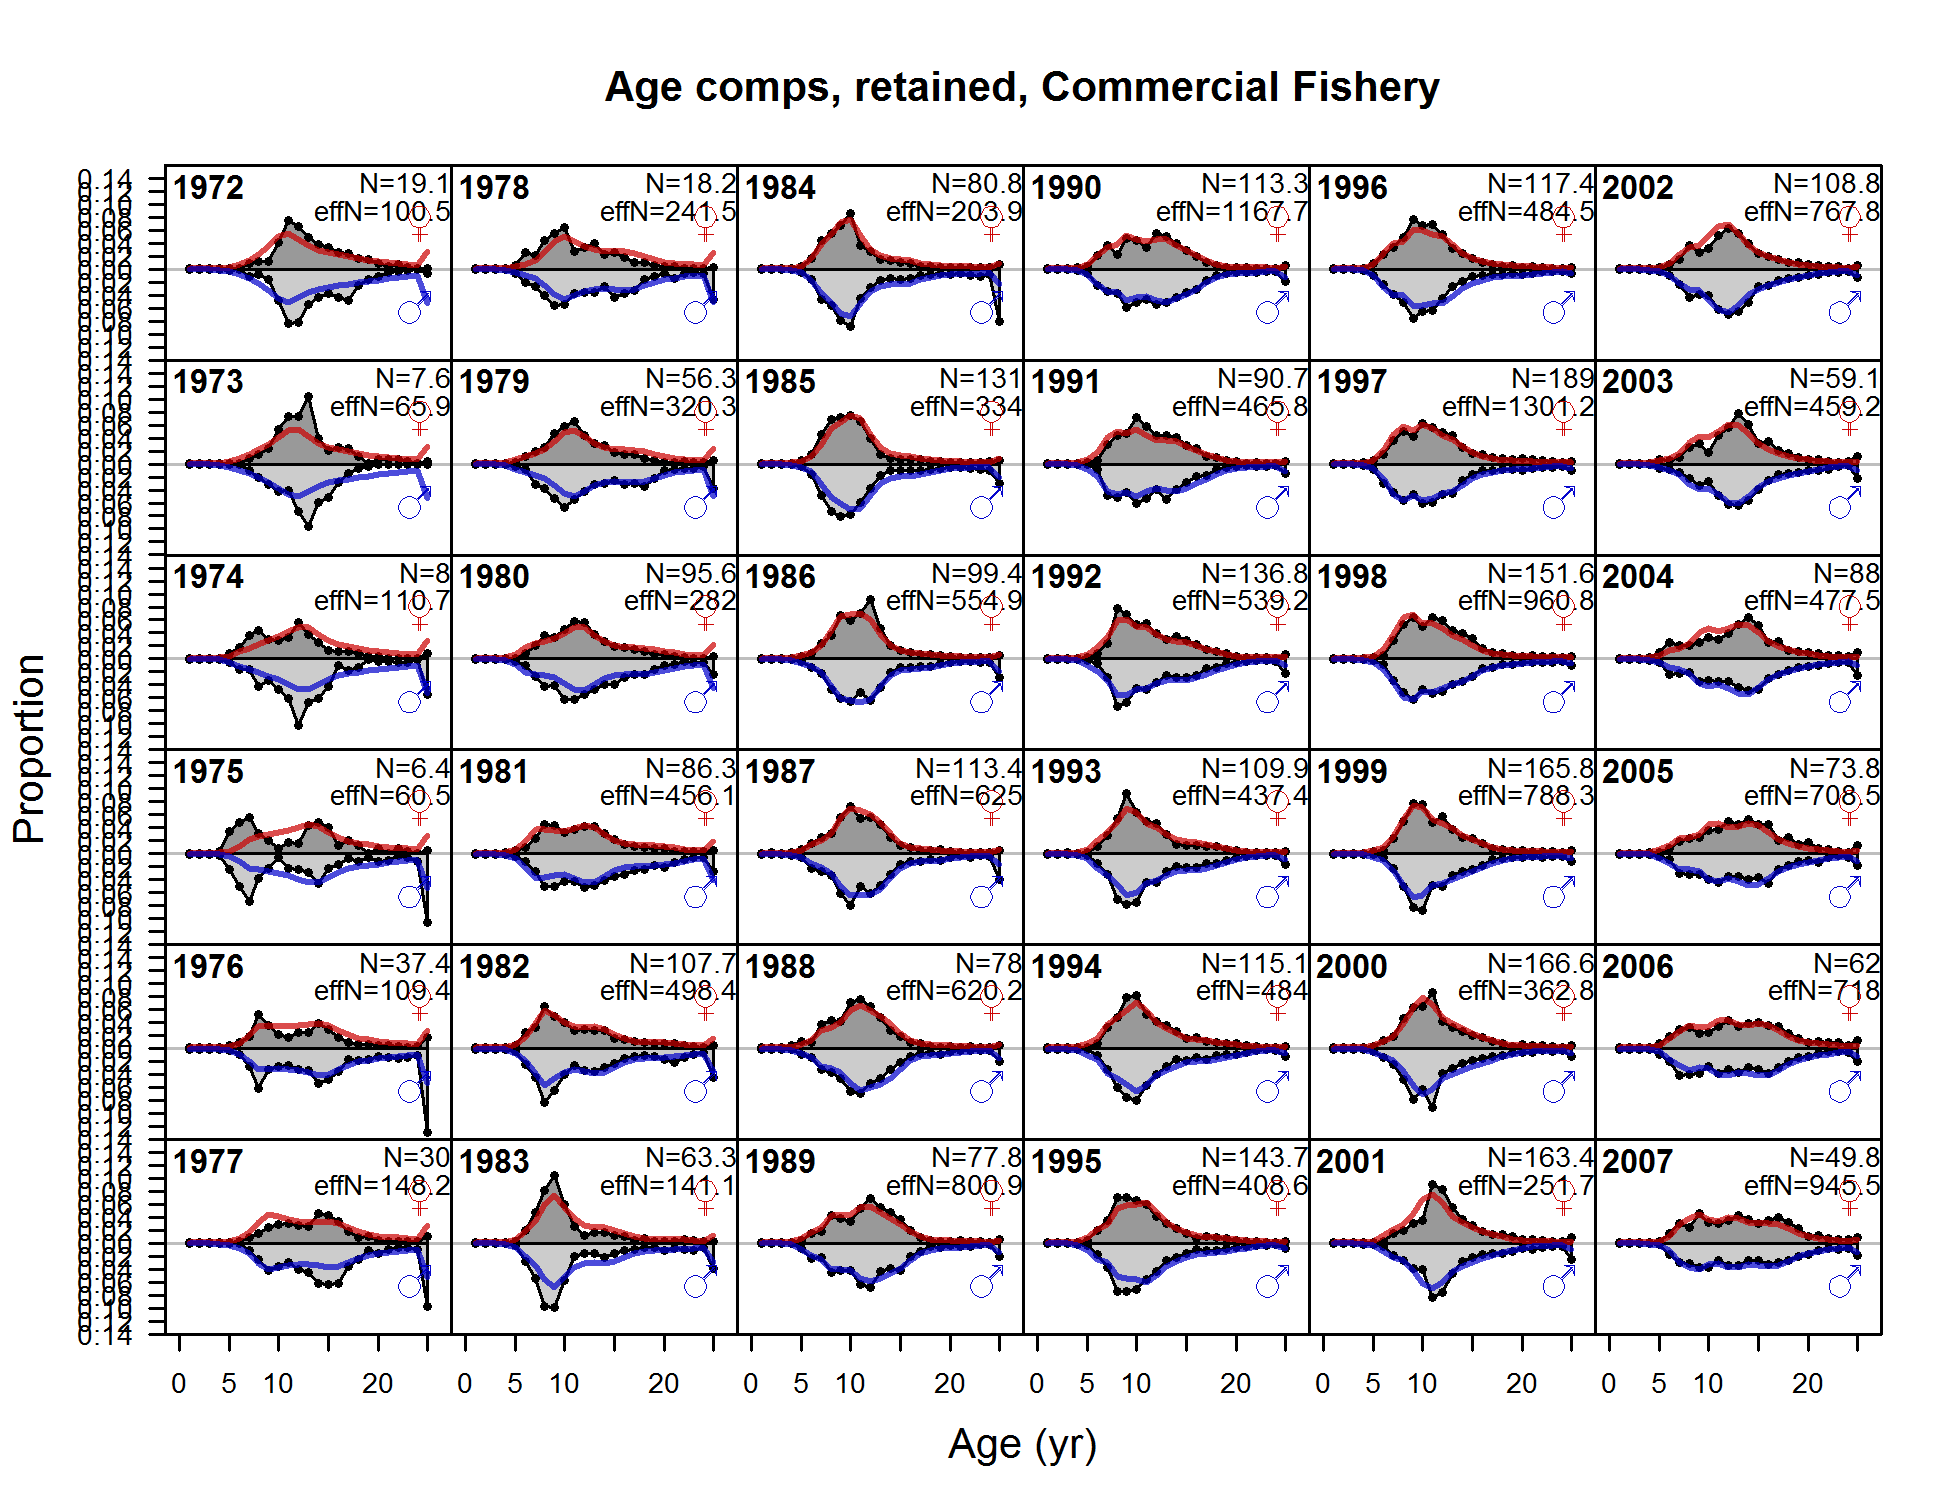
\includegraphics{./r4ss/plots_mod1/comp_agefit_flt1mkt2_page1.png}
\caption{\textbf{Northern model} Age comps, retained, Commercial Fishery
(plot 1 of 2) \label{fig:mod1_1_comp_agefit_flt1mkt2_page1}}
\end{figure}

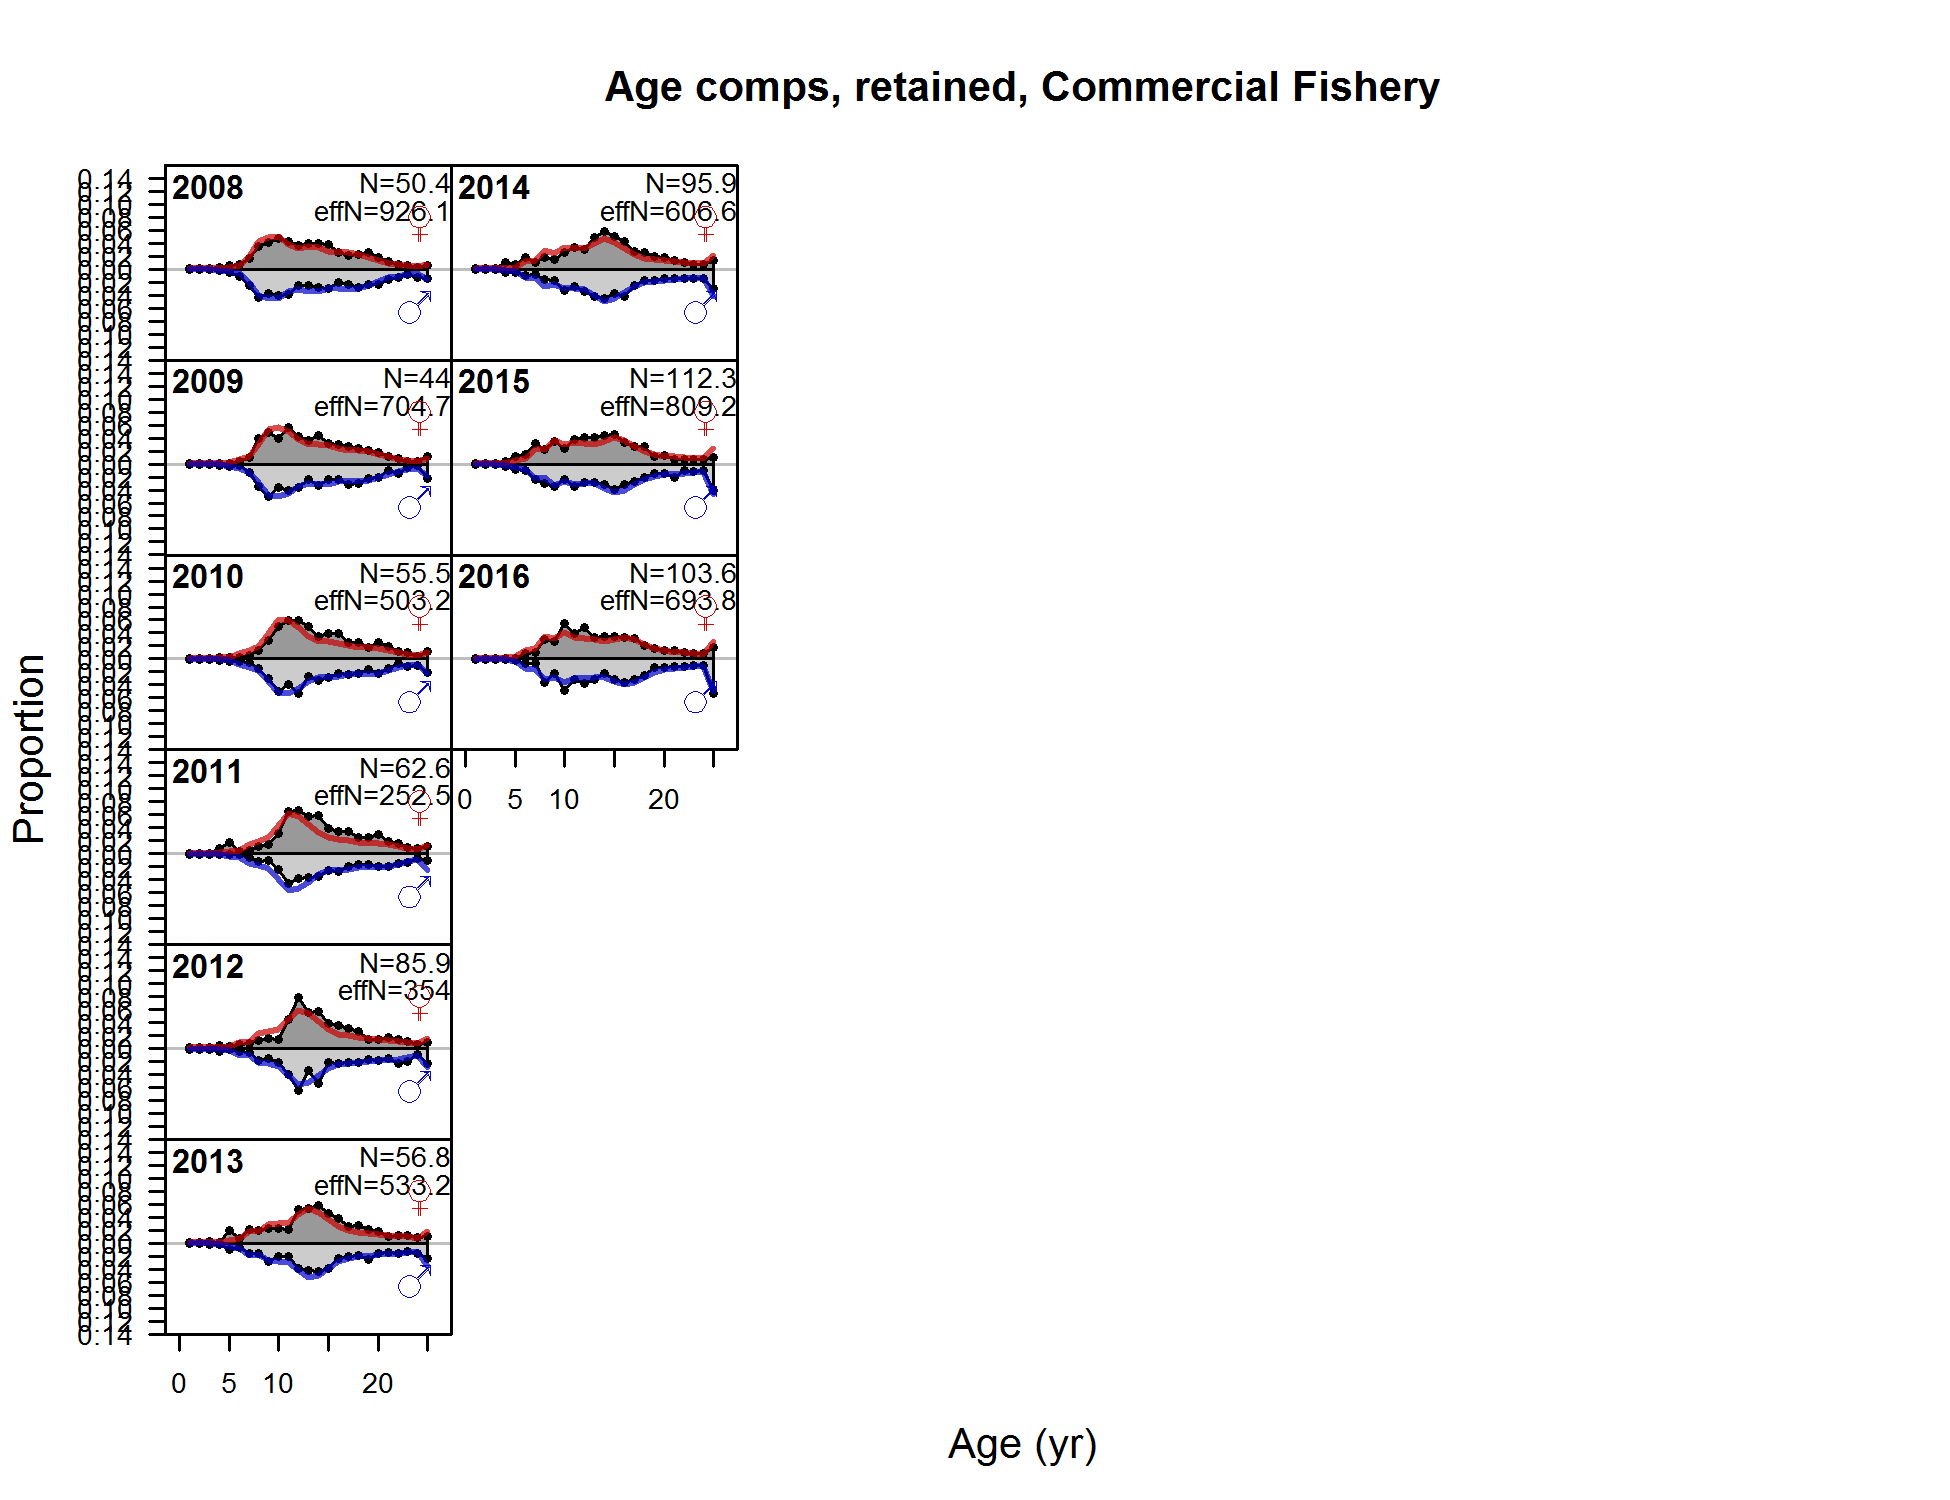
\includegraphics{./r4ss/plots_mod1/comp_agefit_flt1mkt2_page2.png}

\begin{center} 

            Figure continued from previous page 

            \end{center}

\begin{figure}[htbp]
\centering
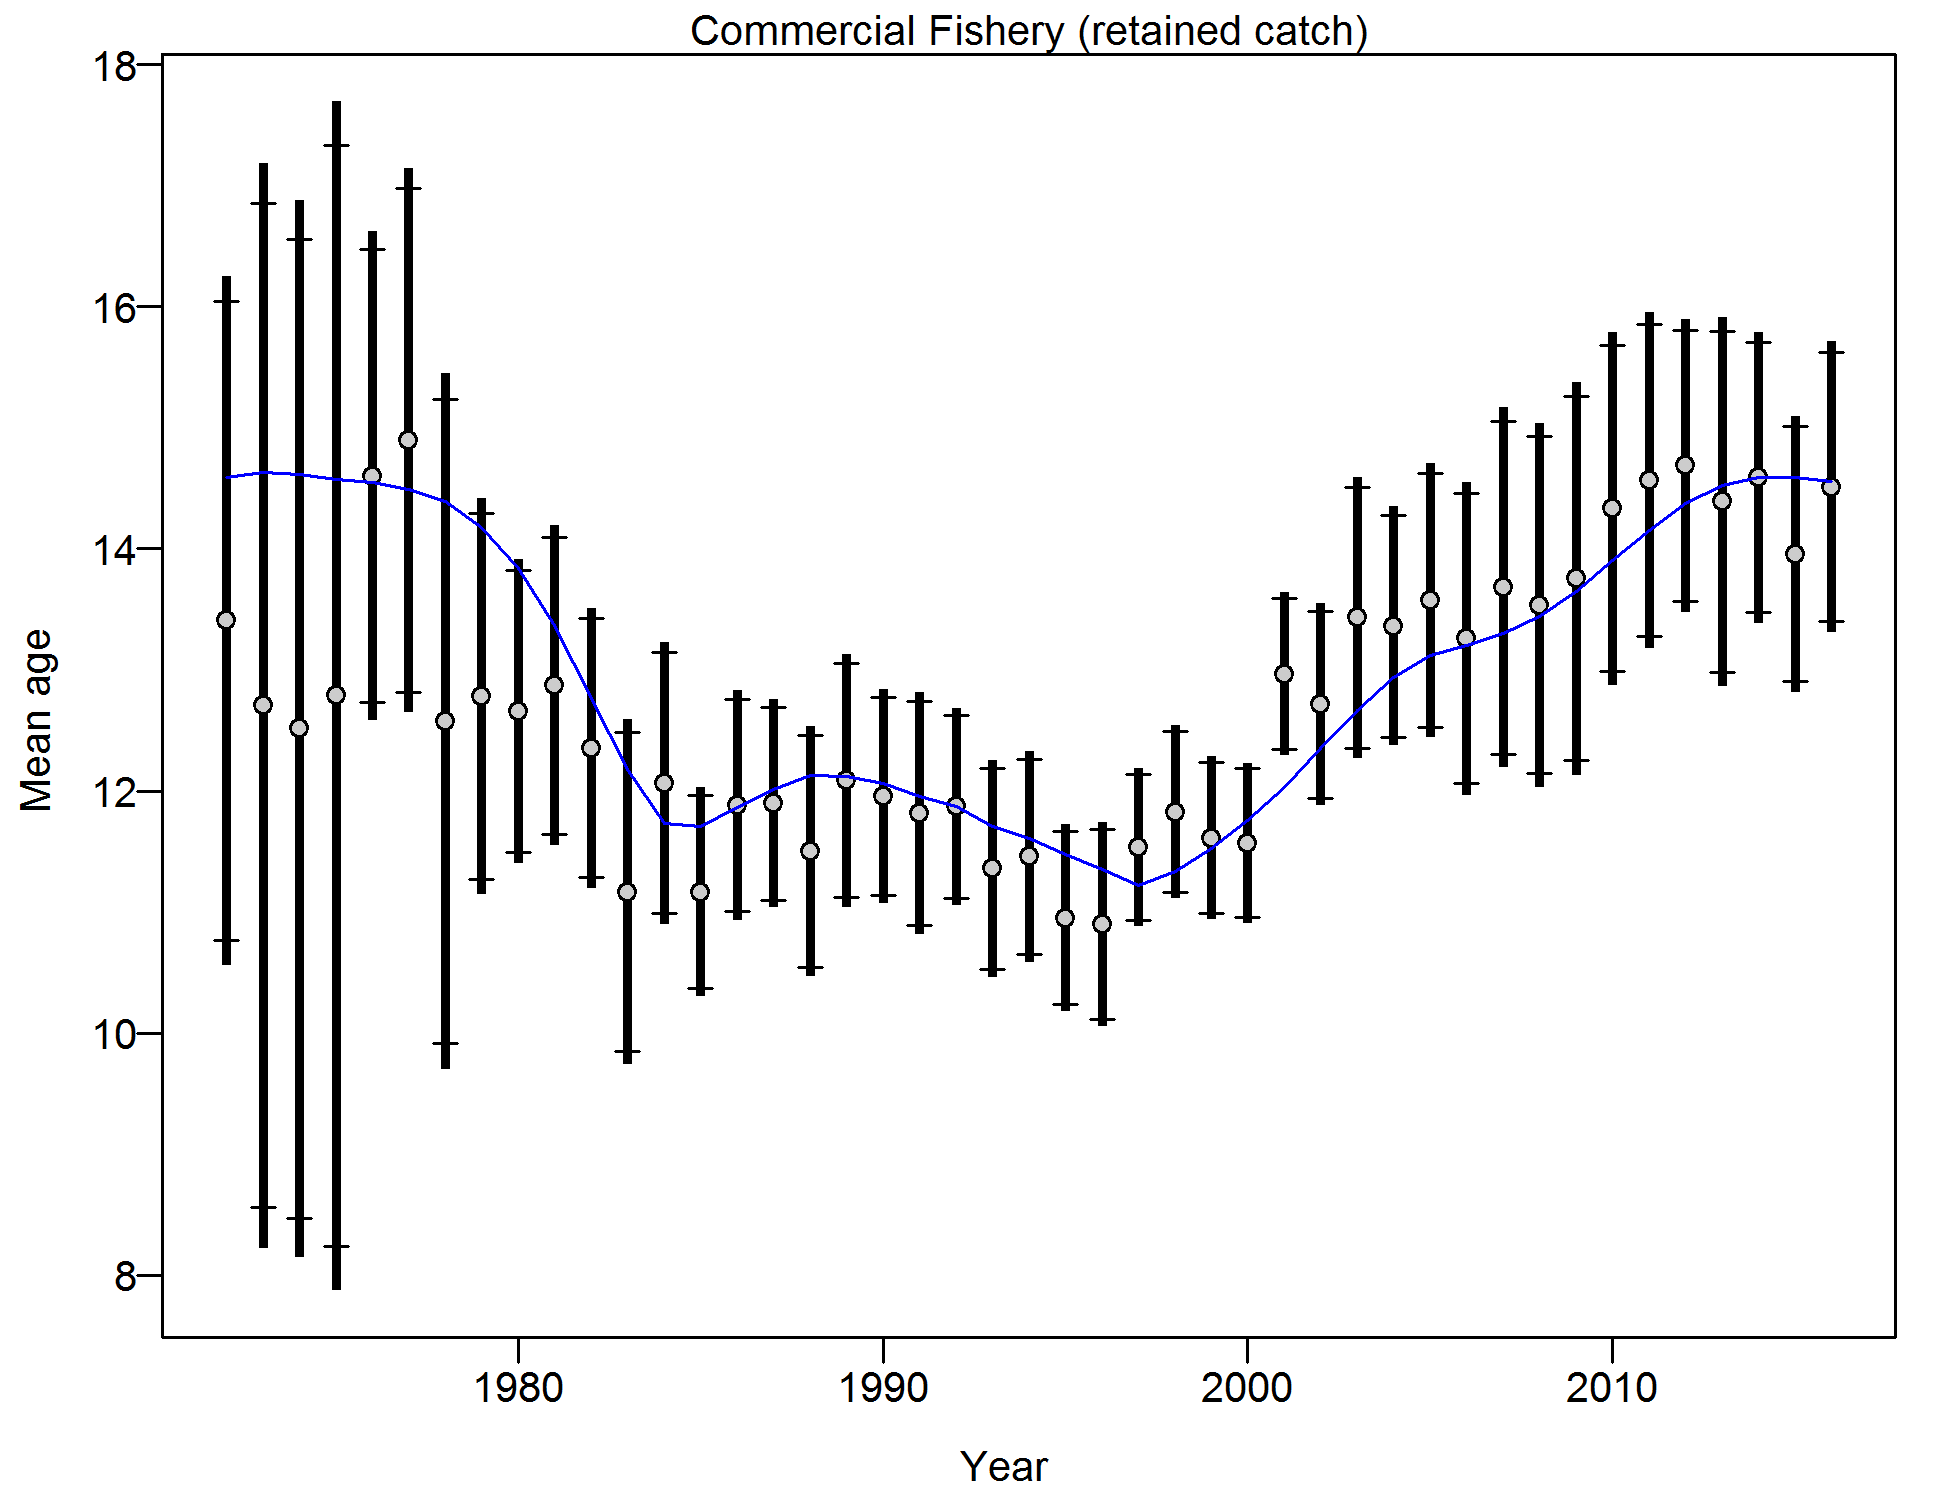
\includegraphics{./r4ss/plots_mod1/comp_agefit_data_weighting_TA1.8_Commercial Fishery.png}
\caption{\textbf{Northern model} Mean age for Commercial Fishery with
95\% confidence intervals based on current samples sizes. Francis data
weighting method TA1.8: thinner intervals (with capped ends) show result
of further adjusting sample sizes based on suggested multiplier (with
95\% interval) for age data from Commercial Fishery: 1.0493
(0.7095\_1.7588) For more info, see Francis, R.I.C.C. (2011). Data
weighting in statistical fisheries stock assessment models. Can. J.
Fish. Aquat. Sci. 68: 1124\_1138.
\label{fig:mod1_5_comp_agefit_data_weighting_TA1.8_Commercial Fishery}}
\end{figure}

\begin{figure}[htbp]
\centering
\includegraphics{./r4ss/plots_mod1/comp_agefit_flt4mkt2.png}
\caption{\textbf{Northern model} Age comps, retained, Recreational WA
\label{fig:mod1_6_comp_agefit_flt4mkt2}}
\end{figure}

\begin{figure}[htbp]
\centering
\includegraphics{./r4ss/plots_mod1/comp_agefit_data_weighting_TA1.8_Recreational WA.png}
\caption{\textbf{Northern model} Mean age for Recreational WA with 95\%
confidence intervals based on current samples sizes. Francis data
weighting method TA1.8: thinner intervals (with capped ends) show result
of further adjusting sample sizes based on suggested multiplier (with
95\% interval) for age data from Recreational WA: 1.0094
(0.6602\_3.0219) For more info, see Francis, R.I.C.C. (2011). Data
weighting in statistical fisheries stock assessment models. Can. J.
Fish. Aquat. Sci. 68: 1124\_1138.
\label{fig:mod1_9_comp_agefit_data_weighting_TA1.8_Recreational WA}}
\end{figure}

\begin{figure}[htbp]
\centering
\includegraphics{./r4ss/plots_mod1/comp_agefit_flt5mkt2.png}
\caption{\textbf{Northern model} Age comps, retained, Triennial Survey
\label{fig:mod1_10_comp_agefit_flt5mkt2}}
\end{figure}

\begin{figure}[htbp]
\centering
\includegraphics{./r4ss/plots_mod1/comp_agefit_data_weighting_TA1.8_Triennial Survey.png}
\caption{\textbf{Northern model} Mean age for Triennial Survey with 95\%
confidence intervals based on current samples sizes. Francis data
weighting method TA1.8: thinner intervals (with capped ends) show result
of further adjusting sample sizes based on suggested multiplier (with
95\% interval) for age data from Triennial Survey: 1.0287
(0.5938\_3.3438) For more info, see Francis, R.I.C.C. (2011). Data
weighting in statistical fisheries stock assessment models. Can. J.
Fish. Aquat. Sci. 68: 1124\_1138.
\label{fig:mod1_13_comp_agefit_data_weighting_TA1.8_Triennial Survey}}
\end{figure}

\begin{figure}[htbp]
\centering
\includegraphics{./r4ss/plots_mod1/comp_agefit__aggregated_across_time.png}
\caption{\textbf{Northern model} Age comps, aggregated across time by
fleet. Labels `retained' and `discard' indicate discarded or retained
sampled for each fleet. Panels without this designation represent the
whole catch. \label{fig:mod1_14_comp_agefit__aggregated_across_time}}
\end{figure}

\begin{figure}[htbp]
\centering
\includegraphics{./r4ss/plots_mod1/comp_gstagefit_flt6mkt2.png}
\caption{\textbf{Northern model} Ghost age comps, retained, NWFSC Combo
Survey \label{fig:mod1_16_comp_gstagefit_flt6mkt2}}
\end{figure}

\FloatBarrier

\newpage

\begin{figure}[htbp]
\centering
\includegraphics{r4ss/plots_mod1/comp_agefit__multi-fleet_comparison.png}
\caption{Age composition Pearson residuals for all fleets in the
Northern model. Closed bubbles are positive residuals (observed
\textgreater{} expected) and open bubbles are negative residuals
(observed \textless{} expected). Bubble colors indicate unsexed fish
(gray), females (red), and males
(blue).\label{fig:comp_Pearson_age_mod1}}
\end{figure}

\FloatBarrier

\newpage

\subsubsection{Fits to conditional-age-at-length compositions for
Northern
model}\label{fits-to-conditional-age-at-length-compositions-for-northern-model}

\begin{figure}[htbp]
\centering
\includegraphics{./r4ss/plots_mod1/comp_condAALfit_data_weighting_TA1.8_condAgeNWFSC Combo Survey.png}
\caption{\textbf{Northern model} Mean age from conditional data
(aggregated across length bins) for NWFSC Combo Survey with 95\%
confidence intervals based on current samples sizes. Francis data
weighting method TA1.8: thinner intervals (with capped ends) show result
of further adjusting sample sizes based on suggested multiplier (with
95\% interval) for conditional age\_at\_length data from NWFSC Combo
Survey: 1.0073 (0.693\_2.3446) For more info, see Francis, R.I.C.C.
(2011). Data weighting in statistical fisheries stock assessment models.
Can. J. Fish. Aquat. Sci. 68: 1124\_1138.
\label{fig:mod1_3_comp_condAALfit_data_weighting_TA1.8_condAgeNWFSC Combo Survey}}
\end{figure}

\begin{figure}[htbp]
\centering
\includegraphics{./r4ss/plots_mod1/comp_condAALfit_Andre_plotsflt6mkt2_page1.png}
\caption{\textbf{Northern model} Conditional AAL plot, retained, NWFSC
Combo Survey (plot 1 of 5) These plots show mean age and std. dev. in
conditional AAL. Left plots are mean AAL by size\_class (obs. and pred.)
with 90\% CIs based on adding 1.64 SE of mean to the data. Right plots
in each pair are SE of mean AAL (obs. and pred.) with 90\% CIs based on
the chi\_square distribution.
\label{fig:mod1_4_comp_condAALfit_Andre_plotsflt6mkt2_page1}}
\end{figure}

\includegraphics{./r4ss/plots_mod1/comp_condAALfit_Andre_plotsflt6mkt2_page2.png}

\begin{center} 

            Figure continued from previous page 

            \end{center}

\includegraphics{./r4ss/plots_mod1/comp_condAALfit_Andre_plotsflt6mkt2_page3.png}

\begin{center} 

            Figure continued from previous page 

            \end{center}

\includegraphics{./r4ss/plots_mod1/comp_condAALfit_Andre_plotsflt6mkt2_page4.png}

\begin{center} 

            Figure continued from previous page 

            \end{center}

\includegraphics{./r4ss/plots_mod1/comp_condAALfit_Andre_plotsflt6mkt2_page5.png}

\begin{center} 

            Figure continued from previous page 

            \end{center}

\FloatBarrier

\newpage

\subsection{Model results for Northern
model}\label{model-results-for-northern-model}

\subsubsection{Base model results for Northern
model}\label{base-model-results-for-northern-model}

\begin{figure}[htbp]
\centering
\includegraphics{r4ss/plots_mod1/ts7_Spawning_output_with_95_asymptotic_intervals_intervals.png}
\caption{Estimated time-series of spawning output for Northern model.
\label{fig:ssb}}
\end{figure}

\FloatBarrier

\begin{figure}[htbp]
\centering
\includegraphics{r4ss/plots_mod1/ts1_Total_biomass_(mt).png}
\caption{Estimated time-series of total biomass for Northern model.
\label{fig:total_bio}}
\end{figure}

\FloatBarrier

\begin{figure}[htbp]
\centering
\includegraphics{r4ss/plots_mod1/ts9_Spawning_depletion_with_95_asymptotic_intervals_intervals.png}
\caption{Estimated time-series of relative biomass for Northern model.
\label{fig:depl}}
\end{figure}

\FloatBarrier

\begin{figure}[htbp]
\centering
\includegraphics{r4ss/plots_mod1/ts11_Age-0_recruits_(1000s)_with_95_asymptotic_intervals.png}
\caption{Estimated time-series of recruitment for the Northern model.
\label{fig:recruits1}}
\end{figure}

\FloatBarrier

\begin{figure}[htbp]
\centering
\includegraphics{r4ss/plots_mod1/recdevs2_withbars.png}
\caption{Estimated time-series of recruitment deviations for the
Northern model. \label{fig:recdevs1}}
\end{figure}

\FloatBarrier

\begin{figure}[htbp]
\centering
\includegraphics{r4ss/plots_mod1/SR_curve2.png}
\caption{Estimated recruitment (red circles) for the Northern model
relative to the stock-recruit relationship (black line). The green line
shows the effect of the bias correction for the lognormal distribution
\label{fig:stock_recruit_curve}}
\end{figure}

\FloatBarrier

\begin{figure}[htbp]
\centering
\includegraphics{Figures/historical_assessment_timeseries.png}
\caption{Comparison of time series of age 4+ biomass for Yellowtail
Rockfish across past assessments. Previous assessments were focused only
on the area north of \(40^\circ 10^\prime\), but also included a small
area within Canada. \label{fig:assessment_history}}
\end{figure}

\FloatBarrier

\newpage

\subsubsection{Sensitivity analyses for Northern
model}\label{sensitivity-analyses-for-northern-model}

\hl{to be added...}

\subsubsection{Likelihood profiles for Northern
model}\label{likelihood-profiles-for-northern-model}

\begin{figure}[htbp]
\centering
\includegraphics{Figures/profiles/profile_logR0.N.png}
\caption{Likelihood profile over the log of equilibrium recruitment
(\(R_0\)) for the Northern model. \label{fig:profile_logR0.N}}
\end{figure}

\FloatBarrier

\begin{figure}[htbp]
\centering
\includegraphics{Figures/profiles/profile_M.N.png}
\caption{Likelihood profile over female natural mortality for the
Northern model. \label{fig:profile_M.N}}
\end{figure}

\FloatBarrier

\begin{figure}[htbp]
\centering
\includegraphics{Figures/profiles/profile_M2.N.png}
\caption{Likelihood profile over the male offset for natural mortality
for the Northern model. Negative values are associated with natural
mortality being lower for males than females.\label{fig:profile_M2.N}}
\end{figure}

\FloatBarrier

\begin{figure}[htbp]
\centering
\includegraphics{Figures/profiles/profile_h.N.png}
\caption{Likelihood profile over stock-recruit steepness (\(h\)) for the
Northern model. \label{fig:profile_h.N}}
\end{figure}

\FloatBarrier

\subsubsection{Retrospective analysis for Northern
model}\label{retrospective-analysis-for-northern-model}

\href{Figures/profiles/retro.N_compare1_spawnbio.png}{Retrospective
analysis of spawning output for the Northern model. \label{fig:retro.N}}

\subsubsection{Forecasts analysis for Northern
model}\label{forecasts-analysis-for-northern-model}

\hl{to be added...}

\FloatBarrier

\newpage

\subsection{Data and model fits for Southern
model}\label{data-and-model-fits-for-southern-model}

\begin{figure}[htbp]
\centering
\includegraphics{r4ss/plots_mod2/data_plot.png}
\caption{Summary of data sources used in the Southern model.
\label{fig:data_plot}}
\end{figure}

\FloatBarrier

\newpage

\begin{figure}[htbp]
\centering
\includegraphics{r4ss/plots_mod2/catch2 landings stacked.png}
\caption{Estimated catch history of Yellowtail Rockfish in the Southern
model. \label{fig:r4ss_catch2_S}}
\end{figure}

\FloatBarrier

\newpage 

\subsubsection{Selectivity, retention, and discards for Southern
model}\label{selectivity-retention-and-discards-for-southern-model}

\begin{figure}[htbp]
\centering
\includegraphics{r4ss/plots_mod2/sel01_multiple_fleets_length1.png}
\caption{Estimated selectivity by length by each fishery and survey in
the Southern model. \label{fig:selex}}
\end{figure}

\FloatBarrier 

\newpage

\subsubsection{Fits to indices of abundance for Southern
model}\label{fits-to-indices-of-abundance-for-southern-model}

\begin{figure}[htbp]
\centering
\includegraphics{r4ss/plots_mod2/index0_all_indices_fit.png}
\caption{Estimated fits to the CPUE and survey indices for the Southern
model. \label{fig:index_fits2}}
\end{figure}

\FloatBarrier 

\newpage

\subsubsection{Length compositions for Southern
model}\label{length-compositions-for-southern-model}

\begin{figure}[htbp]
\centering
\includegraphics{r4ss/plots_mod2/comp_lendat__multi-fleet_comparison.png}
\caption{Length compositions for all fleets in the Southern model.
Bubble size is proportional to proportions within each year.
\label{fig:comp_length_bubble_mod2}}
\end{figure}

\begin{figure}[htbp]
\centering
\includegraphics{./r4ss/plots_mod2/comp_lenfit_flt1mkt2.png}
\caption{\textbf{Southern model} Length comps, retained, Recreational
Fishery \label{fig:mod2_1_comp_lenfit_flt1mkt2}}
\end{figure}

\begin{figure}[htbp]
\centering
\includegraphics{./r4ss/plots_mod2/comp_lenfit_data_weighting_TA1.8_Recreational Fishery.png}
\caption{\textbf{Southern model} Mean length for Recreational Fishery
with 95\% confidence intervals based on current samples sizes. Francis
data weighting method TA1.8: thinner intervals (with capped ends) show
result of further adjusting sample sizes based on suggested multiplier
(with 95\% interval) for len data from Recreational Fishery: 1.0344
(0.6895\_1.9004) For more info, see Francis, R.I.C.C. (2011). Data
weighting in statistical fisheries stock assessment models. Can. J.
Fish. Aquat. Sci. 68: 1124\_1138.
\label{fig:mod2_4_comp_lenfit_data_weighting_TA1.8_Recreational Fishery}}
\end{figure}

\begin{figure}[htbp]
\centering
\includegraphics{./r4ss/plots_mod2/comp_lenfit_flt2mkt2.png}
\caption{\textbf{Southern model} Length comps, retained, Commercial
Fishery \label{fig:mod2_5_comp_lenfit_flt2mkt2}}
\end{figure}

\begin{figure}[htbp]
\centering
\includegraphics{./r4ss/plots_mod2/comp_lenfit_data_weighting_TA1.8_Commercial Fishery.png}
\caption{\textbf{Southern model} Mean length for Commercial Fishery with
95\% confidence intervals based on current samples sizes. Francis data
weighting method TA1.8: thinner intervals (with capped ends) show result
of further adjusting sample sizes based on suggested multiplier (with
95\% interval) for len data from Commercial Fishery: 1.0451
(0.7029\_1.9625) For more info, see Francis, R.I.C.C. (2011). Data
weighting in statistical fisheries stock assessment models. Can. J.
Fish. Aquat. Sci. 68: 1124\_1138.
\label{fig:mod2_8_comp_lenfit_data_weighting_TA1.8_Commercial Fishery}}
\end{figure}

\begin{figure}[htbp]
\centering
\includegraphics{./r4ss/plots_mod2/comp_lenfit_flt3mkt2.png}
\caption{\textbf{Southern model} Length comps, retained, Recreational
Onboard Survey \label{fig:mod2_9_comp_lenfit_flt3mkt2}}
\end{figure}

\begin{figure}[htbp]
\centering
\includegraphics{./r4ss/plots_mod2/comp_lenfit_data_weighting_TA1.8_Recreational Onboard Survey.png}
\caption{\textbf{Southern model} Mean length for Recreational Onboard
Survey with 95\% confidence intervals based on current samples sizes.
Francis data weighting method TA1.8: thinner intervals (with capped
ends) show result of further adjusting sample sizes based on suggested
multiplier (with 95\% interval) for len data from Recreational Onboard
Survey: 1.0273 (0.7124\_1.8741) For more info, see Francis, R.I.C.C.
(2011). Data weighting in statistical fisheries stock assessment models.
Can. J. Fish. Aquat. Sci. 68: 1124\_1138.
\label{fig:mod2_12_comp_lenfit_data_weighting_TA1.8_Recreational Onboard Survey}}
\end{figure}

\begin{figure}[htbp]
\centering
\includegraphics{./r4ss/plots_mod2/comp_lenfit_flt4mkt0.png}
\caption{\textbf{Southern model} Length comps, whole catch, Hook \& Line
Survey \label{fig:mod2_13_comp_lenfit_flt4mkt0}}
\end{figure}

\begin{figure}[htbp]
\centering
\includegraphics{./r4ss/plots_mod2/comp_lenfit_data_weighting_TA1.8_Hook \& Line Survey.png}
\caption{\textbf{Southern model} Mean length for Hook \& Line Survey
with 95\% confidence intervals based on current samples sizes. Francis
data weighting method TA1.8: thinner intervals (with capped ends) show
result of further adjusting sample sizes based on suggested multiplier
(with 95\% interval) for len data from Hook \& Line Survey: 0.9978
(0.6843\_2.3299) For more info, see Francis, R.I.C.C. (2011). Data
weighting in statistical fisheries stock assessment models. Can. J.
Fish. Aquat. Sci. 68: 1124\_1138.
\label{fig:mod2_16_comp_lenfit_data_weighting_TA1.8_Hook & Line Survey}}
\end{figure}

\begin{figure}[htbp]
\centering
\includegraphics{./r4ss/plots_mod2/comp_lenfit_flt5mkt2.png}
\caption{\textbf{Southern model} Length comps, retained, Recreational
Study \label{fig:mod2_17_comp_lenfit_flt5mkt2}}
\end{figure}

\begin{figure}[htbp]
\centering
\includegraphics{./r4ss/plots_mod2/comp_lenfit_data_weighting_TA1.8_Recreational Study.png}
\caption{\textbf{Southern model} Mean length for Recreational Study with
95\% confidence intervals based on current samples sizes. Francis data
weighting method TA1.8: thinner intervals (with capped ends) show result
of further adjusting sample sizes based on suggested multiplier (with
95\% interval) for len data from Recreational Study: 1.0852
(0.5552\_14.1578) For more info, see Francis, R.I.C.C. (2011). Data
weighting in statistical fisheries stock assessment models. Can. J.
Fish. Aquat. Sci. 68: 1124\_1138.
\label{fig:mod2_20_comp_lenfit_data_weighting_TA1.8_Recreational Study}}
\end{figure}

\begin{figure}[htbp]
\centering
\includegraphics{./r4ss/plots_mod2/comp_lenfit__aggregated_across_time.png}
\caption{\textbf{Southern model} Length comps, aggregated across time by
fleet. Labels `retained' and `discard' indicate discarded or retained
sampled for each fleet. Panels without this designation represent the
whole catch. \label{fig:mod2_21_comp_lenfit__aggregated_across_time}}
\end{figure}

\FloatBarrier

\newpage

\begin{figure}[htbp]
\centering
\includegraphics{r4ss/plots_mod2/comp_lenfit__multi-fleet_comparison.png}
\caption{Length composition Pearson residuals for all fleets in the
Southern model. Closed bubbles are positive residuals (observed
\textgreater{} expected) and open bubbles are negative residuals
(observed \textless{} expected). \label{fig:comp_Pearson_length_mod2}}
\end{figure}

\FloatBarrier

\newpage

\subsubsection{Age compositions for Southern
model}\label{age-compositions-for-southern-model}

\begin{figure}[htbp]
\centering
\includegraphics{r4ss/plots_mod2/comp_agedat__multi-fleet_comparison.png}
\caption{Age compositions for all fleets in the Southern model. Bubble
size is proportional to proportions within each year.
\label{fig:comp_age_bubble_mod2}}
\end{figure}

\FloatBarrier

\newpage

\begin{figure}[htbp]
\centering
\includegraphics{./r4ss/plots_mod2/comp_agefit_flt1mkt2.png}
\caption{\textbf{Southern model} Age comps, retained, Recreational
Fishery \label{fig:mod2_1_comp_agefit_flt1mkt2}}
\end{figure}

\begin{figure}[htbp]
\centering
\includegraphics{./r4ss/plots_mod2/comp_agefit_data_weighting_TA1.8_Recreational Fishery.png}
\caption{\textbf{Southern model} Mean age for Recreational Fishery with
95\% confidence intervals based on current samples sizes. Francis data
weighting method TA1.8: thinner intervals (with capped ends) show result
of further adjusting sample sizes based on suggested multiplier (with
95\% interval) for age data from Recreational Fishery: 0.925
(0.4929\_24.4689) For more info, see Francis, R.I.C.C. (2011). Data
weighting in statistical fisheries stock assessment models. Can. J.
Fish. Aquat. Sci. 68: 1124\_1138.
\label{fig:mod2_4_comp_agefit_data_weighting_TA1.8_Recreational Fishery}}
\end{figure}

\begin{figure}[htbp]
\centering
\includegraphics{./r4ss/plots_mod2/comp_agefit_flt4mkt0.png}
\caption{\textbf{Southern model} Age comps, whole catch, Hook \& Line
Survey \label{fig:mod2_5_comp_agefit_flt4mkt0}}
\end{figure}

\begin{figure}[htbp]
\centering
\includegraphics{./r4ss/plots_mod2/comp_agefit_data_weighting_TA1.8_Hook \& Line Survey.png}
\caption{\textbf{Southern model} Mean age for Hook \& Line Survey with
95\% confidence intervals based on current samples sizes. Francis data
weighting method TA1.8: too few points to calculate adjustments. For
more info, see Francis, R.I.C.C. (2011). Data weighting in statistical
fisheries stock assessment models. Can. J. Fish. Aquat. Sci. 68:
1124\_1138.
\label{fig:mod2_8_comp_agefit_data_weighting_TA1.8_Hook & Line Survey}}
\end{figure}

\begin{figure}[htbp]
\centering
\includegraphics{./r4ss/plots_mod2/comp_agefit__aggregated_across_time.png}
\caption{\textbf{Southern model} Age comps, aggregated across time by
fleet. Labels `retained' and `discard' indicate discarded or retained
sampled for each fleet. Panels without this designation represent the
whole catch. \label{fig:mod2_9_comp_agefit__aggregated_across_time}}
\end{figure}

\begin{figure}[htbp]
\centering
\includegraphics{./r4ss/plots_mod2/comp_gstagefit_flt2mkt2.png}
\caption{\textbf{Southern model} Ghost age comps, retained, Commercial
Fishery \label{fig:mod2_11_comp_gstagefit_flt2mkt2}}
\end{figure}

\begin{figure}[htbp]
\centering
\includegraphics{r4ss/plots_mod2/comp_agefit__multi-fleet_comparison.png}
\caption{Age composition Pearson residuals for all fleets in the
Southern model. Closed bubbles are positive residuals (observed
\textgreater{} expected) and open bubbles are negative residuals
(observed \textless{} expected). \label{fig:comp_Pearson_age_mod2}}
\end{figure}

\FloatBarrier

\newpage

\subsubsection{Fits to conditional-age-at-length compositions for
Southern
model}\label{fits-to-conditional-age-at-length-compositions-for-southern-model}

\begin{figure}[htbp]
\centering
\includegraphics{./r4ss/plots_mod2/comp_condAALfit_data_weighting_TA1.8_condAgeCommercial Fishery.png}
\caption{\textbf{Southern model} Mean age from conditional data
(aggregated across length bins) for Commercial Fishery with 95\%
confidence intervals based on current samples sizes. Francis data
weighting method TA1.8: thinner intervals (with capped ends) show result
of further adjusting sample sizes based on suggested multiplier (with
95\% interval) for conditional age\_at\_length data from Commercial
Fishery: 0.8567 (0.5727\_1.8556) For more info, see Francis, R.I.C.C.
(2011). Data weighting in statistical fisheries stock assessment models.
Can. J. Fish. Aquat. Sci. 68: 1124\_1138.
\label{fig:mod2_4_comp_condAALfit_data_weighting_TA1.8_condAgeCommercial Fishery}}
\end{figure}

\begin{figure}[htbp]
\centering
\includegraphics{./r4ss/plots_mod2/comp_condAALfit_Andre_plotsflt2mkt2_page1.png}
\caption{\textbf{Southern model} Conditional AAL plot, retained,
Commercial Fishery (plot 1 of 8) These plots show mean age and std. dev.
in conditional AAL. Left plots are mean AAL by size\_class (obs. and
pred.) with 90\% CIs based on adding 1.64 SE of mean to the data. Right
plots in each pair are SE of mean AAL (obs. and pred.) with 90\% CIs
based on the chi\_square distribution.
\label{fig:mod2_5_comp_condAALfit_Andre_plotsflt2mkt2_page1}}
\end{figure}

\includegraphics{./r4ss/plots_mod2/comp_condAALfit_Andre_plotsflt2mkt2_page2.png}

\begin{center} 

            Figure continued from previous page 

            \end{center}

\includegraphics{./r4ss/plots_mod2/comp_condAALfit_Andre_plotsflt2mkt2_page3.png}

\begin{center} 

            Figure continued from previous page 

            \end{center}

\includegraphics{./r4ss/plots_mod2/comp_condAALfit_Andre_plotsflt2mkt2_page4.png}

\begin{center} 

            Figure continued from previous page 

            \end{center}

\includegraphics{./r4ss/plots_mod2/comp_condAALfit_Andre_plotsflt2mkt2_page5.png}

\begin{center} 

            Figure continued from previous page 

            \end{center}

\includegraphics{./r4ss/plots_mod2/comp_condAALfit_Andre_plotsflt2mkt2_page6.png}

\begin{center} 

            Figure continued from previous page 

            \end{center}

\includegraphics{./r4ss/plots_mod2/comp_condAALfit_Andre_plotsflt2mkt2_page7.png}

\begin{center} 

            Figure continued from previous page 

            \end{center}

\includegraphics{./r4ss/plots_mod2/comp_condAALfit_Andre_plotsflt2mkt2_page8.png}

\begin{center} 

            Figure continued from previous page 

            \end{center}

\FloatBarrier

\newpage

\subsection{Model results for Southern
model}\label{model-results-for-southern-model}

\subsubsection{Base model results for Southern
model}\label{base-model-results-for-southern-model}

\begin{figure}[htbp]
\centering
\includegraphics{r4ss/plots_mod2/ts7_Spawning_output_with_95_asymptotic_intervals_intervals.png}
\caption{Estimated time-series of spawning output for Southern model.
\label{fig:ssb}}
\end{figure}

\FloatBarrier

\begin{figure}[htbp]
\centering
\includegraphics{r4ss/plots_mod2/ts1_Total_biomass_(mt).png}
\caption{Estimated time-series of total biomass for Southern model.
\label{fig:total_bio}}
\end{figure}

\FloatBarrier

\begin{figure}[htbp]
\centering
\includegraphics{r4ss/plots_mod2/ts9_Spawning_depletion_with_95_asymptotic_intervals_intervals.png}
\caption{Estimated time-series of relative biomass for Southern model.
\label{fig:depl}}
\end{figure}

\FloatBarrier

\begin{figure}[htbp]
\centering
\includegraphics{r4ss/plots_mod2/ts11_Age-0_recruits_(1000s)_with_95_asymptotic_intervals.png}
\caption{Estimated time-series of recruitment for the Southern model.
\label{fig:recruits1}}
\end{figure}

\FloatBarrier

\begin{figure}[htbp]
\centering
\includegraphics{r4ss/plots_mod2/recdevs2_withbars.png}
\caption{Estimated time-series of recruitment deviations for the
Southern model. \label{fig:recdevs1}}
\end{figure}

\FloatBarrier

\begin{figure}[htbp]
\centering
\includegraphics{r4ss/plots_mod2/SR_curve2.png}
\caption{Estimated recruitment (red circles) for the Southern model
relative to the stock-recruit relationship (black line). The green line
shows the effect of the bias correction for the lognormal distribution
\label{fig:stock_recruit_curve}}
\end{figure}

\FloatBarrier

\newpage

\subsubsection{Sensitivity analyses for Southern
model}\label{sensitivity-analyses-for-southern-model}

\hl{to be added...}

\subsubsection{Likelihood profiles for Southern
model}\label{likelihood-profiles-for-southern-model}

\begin{figure}[htbp]
\centering
\includegraphics{Figures/profiles/profile_logR0.S.png}
\caption{Likelihood profile over the log of equilibrium recruitment
(\(R_0\)) for the Southern model. \label{fig:profile_logR0.S}}
\end{figure}

\FloatBarrier

\begin{figure}[htbp]
\centering
\includegraphics{Figures/profiles/profile_M.S.png}
\caption{Likelihood profile over female natural mortality for the
Southern model. \label{fig:profile_M.S}}
\end{figure}

\FloatBarrier

\begin{figure}[htbp]
\centering
\includegraphics{Figures/profiles/profile_M2.S.png}
\caption{Likelihood profile over the male offset for natural mortality
for the Southern model. Negative values are associated with natural
mortality being lower for males than females.\label{fig:profile_M2.S}}
\end{figure}

\FloatBarrier

\begin{figure}[htbp]
\centering
\includegraphics{Figures/profiles/profile_h.S.png}
\caption{Likelihood profile over stock-recruit steepness (\(h\)) for the
Southern model. \label{fig:profile_h.S}}
\end{figure}

\FloatBarrier

\subsubsection{Retrospective analysis for Southern
model}\label{retrospective-analysis-for-southern-model}

\href{Figures/profiles/retro.S_compare1_spawnbio.png}{Retrospective
analysis of spawning output for the Southern model. \label{fig:retro.S}}

\subsubsection{Forecasts analysis for Southern
model}\label{forecasts-analysis-for-southern-model}

\hl{to be added...}

\FloatBarrier

\newpage

\color{black}

\section*{References}\label{references}
\addcontentsline{toc}{section}{References}

\renewcommand{\thepage}{}




\newpage

\hypertarget{refs}{}
\hypertarget{ref-Alverson1964}{}
Alverson, D.L., Pruter, a T., and Ronholt, L.L. 1964. A Study of
Demersal Fishes and Fisheries of the Northeastern Pacific Ocean.
Institute of Fisheries, University of British Columbia.

\hypertarget{ref-AFSC2016}{}
Center, A.F.S. 2016. Assessment of the Other Rockfish stock complex in
the Gulf of Alaska. Available from
\url{https://www.afsc.noaa.gov/REFM/Docs/2016/GOAorock.pdf} {[}accessed
18 June 2017{]}.

\hypertarget{ref-Cope2013}{}
Cope, J., Dick, E., MacCall, A., Monk, M., Soper, B., and Wetzel, C.
2013. Data-moderate stock assessments for brown, china, copper,
sharpchin, stripetail, and yellowtail rockfishes and english and rex
soles in 2013. National Oceanic and Atmospheric Administration, National
Marine Fisheries Service.

\hypertarget{ref-PFMC2016}{}
Council, P.F.M. 2016. STATUS OF THE PACIFIC COAST GROUNDFISH FISHERY.
Available from
\url{http://www.pcouncil.org/wp-content/uploads/2017/02/SAFE_Dec2016_02_28_2017.pdf}
{[}accessed 18 June 2017{]}.

\hypertarget{ref-Dick2017}{}
Dick, E., Beyer, S., Mangel, M., and Ralston, S. 2017. A meta-analysis
of fecundity in rockfishes (genus sebastes). Fisheries Research
\textbf{187}: 73--85. Elsevier.

\hypertarget{ref-Eldridge1991}{}
Eldridge, M.B., Whipple, J.A., Bowers, M.J., Jarvis, B.M., and Gold, J.
1991. Reproductive performance of yellowtail rockfish, sebastes
flavidus. Environmental biology of fishes \textbf{30}(1): 91--102.
Springer.

\hypertarget{ref-Fournier2012}{}
Fournier, D.A., Skaug, H.J., Ancheta, J., Ianelli, J., Magnusson, A.,
Maunder, M.N., Nielsen, A., and Sibert, J. 2012. AD model builder: Using
automatic differentiation for statistical inference of highly
parameterized complex nonlinear models. Optimization Methods and
Software \textbf{27}(2): 233--249. Taylor \& Francis.

\hypertarget{ref-Fraidenburg1980}{}
Fraidenburg, M. 1980. YELLOWTAIL rockfish, sebastes-flavidus, length and
age composition off california, oregon, and washington in 1977. MARINE
FISHERIES REVIEW \textbf{42}(3-4): 54--56. NATL MARINE FISHERIES SERVICE
SCIENTIFIC PUBL OFFICE 7600 SAND POINT WAY NE BIN C15700, SEATTLE, WA
98115.

\hypertarget{ref-Francis2011}{}
Francis, R. 2011. Data weighting in statistical fisheries stock
assessment models. Canadian Journal of Fisheries and Aquatic Sciencies
\textbf{68}: 1124--1138.

\hypertarget{ref-Hamel2015}{}
Hamel, O. 2015. A method for calculating a meta-analytical prior for the
natural mortality rate using multiple life history correlates. ICES
Journal of Marine Science \textbf{72}: 62--69.

\hypertarget{ref-Harry1961}{}
Harry, G., and Morgan, A. 1961. History of the trawl fishery, 1884-1961.
Oregon Fish Commission Research Briefs \textbf{19}: 5--26.

\hypertarget{ref-Hess2011}{}
Hess, J., Vetter, R., and Moran, P. (n.d.). A steep genetic cline in
yellowtail rockfish, \emph{\{}Sebastes flavidus, suggests regional
isolation across the cape mendocino faunal break. Canadian Journal of
Fisheries and Aquatic Sciences: 89--104.

\hypertarget{ref-Lai2003}{}
Lai, H., Tagart, J., Ianelli, J., and Wallace, F. 2003. Status of the
yellowtail rockfish resource in 2003. Status of the Pacific Coast
groundfish fishery through.

\hypertarget{ref-Love2002}{}
Love, M., Yoklavich, M., and Thorsteinson, L. 2002. The rockfishes of
the northeast Pacific. University of California Press, Berkeley, CA,
USA.

\hypertarget{ref-Love2011}{}
Love, M.S. 2011. Certainly more than you want to know about the fishes
of the pacific coast: A postmodern experience. Really Big Press.

\hypertarget{ref-Marks2015}{}
Marks, C.I., Fields, R.T., Starr, R.M., Field, J.C., Miller, R.R.,
Beyer, S.G., Sogard, S.M., Miller, R.R., Beyer, S.G., Wilson-Vandenberg,
D., and others. 2015. Changes in size composition and relative abundance
of fishes in central california after a decade of spatial fishing
closures. CALIFORNIA COOPERATIVE OCEANIC FISHERIES INVESTIGATIONS
REPORTS \textbf{56}: 119--132. SCRIPPS INST OCEANOGRAPHY A-003, LA
JOLLA, CA 92093 USA.

\hypertarget{ref-McAllister1997}{}
McAllister, M.K., and Ianelli, J.N. 1997. Bayesian stock assessment
using catch-age data and the sampling - importance resampling algorithm.
Canadian Journal of Fisheries and Aquatic Sciences \textbf{54}(2):
284--300.

\hypertarget{ref-Methot2015}{}
Methot, R.D. 2015. User manual for Stock Synthesis model version 3.24s.
NOAA Fisheries, US Department of Commerce.

\hypertarget{ref-Pikitch1988}{}
Pikitch, E., Erickson, D., and Wallace, J. 1988. An evaluation of the
effectiveness of trip limits as a management tool. Northwest and Alaska
Fisheries Center, National Marine Fisheries Service, US Department of
Commerce.

\hypertarget{ref-Rogers1992}{}
Rogers, J., and Pikitch, E. 1992. Numerical definition of groundfish
assemblages caught off the coasts of Oregon and Washington using
commercial fishing strategies. Canadian Journal of Fisheries and and
Aquatic Sciences \textbf{49}: 2648--2656.

\hypertarget{ref-Stephens2004}{}
Stephens, A., and MacCall, A. 2004. A multispecies approach to
subsetting logbook data for purposes of estimating CPUE. Fisheries
Research \textbf{70}: 299--310.

\hypertarget{ref-Tagart1982}{}
Tagart, J. 1982. Status of the yellowtail rockfish (sebastes flavidus)
fishery. State of Washington, Department of Fisheries.

\hypertarget{ref-Tagart1991}{}
Tagart, J. 1991. Population dynamics of yellowtail rockfish (sebastes
flavidus) stocks in the northem california to southwest vancouver island
region. Ph. D\_ thesis, University of Wash-ington, Seattle.

\hypertarget{ref-Tagart1997}{}
Tagart, J., Ianelli, J., Hoffman, A., and Wallace, F. 1997. Status of
the yellowtail rockfish resource in 1997. Pacific Fishery Management
Council, Portland, OR.

\hypertarget{ref-Tagart2000}{}
Tagart, J., Wallace, F., and Ianelli, J.N. 2000. Status of the
yellowtail rockfish resource in 2000. Pacific Fishery Management
Council.

\hypertarget{ref-Tagart1988}{}
Tagart, J.V. 1988. Status of the yellowtail rockfish stocks in the
international north pacific fishery commission vancouver and columbia
areas. Department of Fish; Wildlife.

\hypertarget{ref-Then2014}{}
Then, A.Y., Hoenig, J.M., Hall, N.G., and Hewitt, D.A. 2014. Evaluating
the predictive performance of empirical estimators of natural mortality
rate using information on over 200 fish species. ICES Journal of Marine
Science \textbf{72}(1): 82--92. ICES/CIEM.

\hypertarget{ref-Wallace2005}{}
Wallace, J., and Lai, H.-L. 2005. Status of the Yellowtail Rockfish in
2004. \emph{In} Human Biology. Pacific Fisheries Management Council,
Portland, OR.

\end{document}
